% This template was originally by R. Jacob Vogelstein
% Updated on March 1, 2010 by Noah J. Cowan
% Finally put to use by Andrew Whitbeck 2013
% Copied by Christopher B Martin on Jan. 5, 2015 for use in Thesis writing

\documentclass[12pt,twoside,final]{thesis}

% FOR FINAL VERSON CHANGE TO [oneside,final]

\usepackage{mathtools}
\usepackage{setspace}
\usepackage{feynmp}
\usepackage{rotating}
\usepackage{cite}
\usepackage{multirow}
\usepackage{amsmath,amsfonts}
\usepackage{amssymb}
\usepackage{graphicx}
\usepackage{epstopdf}
\usepackage{physics}
\usepackage{slashed}
\usepackage{hepunits}
\usepackage{SIunits}
\usepackage{mathrsfs}
\usepackage{contour}
\usepackage{color}
\usepackage{fixltx2e}
\usepackage{array}
% wrapfig is fragile: use sparingly
\usepackage{wrapfig} 
\usepackage{courier}  % Use this for ugly fonts
\usepackage[section]{placeins}

%%Added by Chris

\DeclareGraphicsRule{*}{mps}{*}{}
\usepackage{xcolor}

%My Colors
\definecolor{UniBlue}{rgb}{0.05,0.12,0.38}
\definecolor{myblue}{rgb}{0.,0.,1.}
\definecolor{myred}{rgb}{0.94,0.,0.11}
\definecolor{mygreen}{rgb}{0.13,0.44,0.07}
\definecolor{puregreen}{rgb}{0.00,1.00,0.00}
\definecolor{mygrey}{rgb}{0.39,0.39,0.39}
\definecolor{myviolet}{rgb}{0.44,0.,0.70}
\definecolor{4Lblue}{rgb}{0.47,0.67,0.88}
\definecolor{4Lgreen}{rgb}{0.33,0.54,0.33}
\definecolor{mygray}{gray}{0.30}

\definecolor{CV_Dark}{HTML}{244BFC}
\definecolor{CV_Light}{HTML}{5977FF}

\contourlength{0.5pt} %how thick each copy is
\contournumber{20}  %number of copies

%Forces figures and other floating objects to be placed within a specific subsection.
\makeatletter
\AtBeginDocument{%
  \expandafter\renewcommand\expandafter\subsection\expandafter{%
    \expandafter\@fb@secFB\subsection
  }%
}
\makeatother

%end Added by Chris


\usepackage{fancyhdr}    % Use nice looking headers along with the required footer page numbers   
%\usepackage[hypertex]{hyperref}

%Define the header/footer style
\pagestyle{fancy}
\fancyhf{}
\setlength{\headheight}{15pt}
\lhead{\leftmark}
\cfoot{\thepage}
\renewcommand{\headrulewidth}{0pt}
\fancypagestyle{plain}{% Redefine ``plain'' style for chapter boundaries
\fancyhf{} % clear all header and footer fields
\fancyfoot[C]{\thepage} % except the center
\renewcommand{\headrulewidth}{0pt}
\renewcommand{\footrulewidth}{0pt}}

%\tolerance=10000

%\makeglossary % enable the glossary

\begin{document}

\title{Discovery and Characterization of a Higgs boson using four-lepton events from the CMS experiment}
\author{Christopher B. Martin}
\degreemonth{July}
\degreeyear{2015} 
\dissertation
\doctorphilosophy
\copyrightnotice

% add your chaptders, best way is to have separate TeX files for each chapter
%% FRONTMATTER
\begin{frontmatter}

% generate title
\maketitle

\begin{abstract}
ABSTRACT

\vspace{.3cm}
\noindent Primary Reader: Andrei Gritsan\\
Secondary Reader:

\end{abstract}

\begin{acknowledgement}

THANKS TO

\end{acknowledgement}

%\begin{dedication} 

%\end{dedication}

% generate table of contents
\tableofcontents

% generate list of tables
\listoftables

% generate list of figures
\listoffigures

\end{frontmatter}
\chapter{Introduction}
\label{sec:intro}
\chaptermark{Introduction}

This is a sample equation:
\begin{equation}
\mathscr{L}_{EM} = \bar{\psi}\left(i\gamma^{\mu}(\partial_{\mu}+ieA_{\mu})-m\right)\psi - \frac{1}{4}F_{\mu\nu}F^{\mu\nu}.
\label{eq:EMlagrangian}
\end{equation}


This is a sample Feynman Diagram:

\begin{figure}
\begin{center}
\unitlength=1mm
\begin{fmffile}{eeScattering}

\begin{fmfgraph*}(40,30) \fmfpen{thick}
  \fmfleft{i1,i2} \fmfright{sp1,sp2}
  \fmf{fermion,label=$e^-$}{i1,v1,sp1} 
  \fmf{fermion,label=$e^-$}{i2,v2,sp2}
  \fmf{photon,label=$\gamma$}{v1,v2}
\end{fmfgraph*}

\end{fmffile}
\end{center}
\caption{Feynman diagram depicting electron-electron scattering via
the electromagnetic interaction.}
\label{fig:eeScattering}
\end{figure}

This is a sample table:

\begin{table}
\begin{center}
\begin{tabular}{l|c|c|c|c}
\hline 
\hline
particle & Q  & $T_3$ & $Y_W$ & colored \\ \hline \hline
$e_L$, $\mu_L$, $\tau_L$  & -1 & -1/2   &  -1 &  no \\ 
$e_R$, $\mu_R$, $\tau_R$  & -1 & 0      &  -2 &  no \\ 
$\nu_L$  & 0   & 1/2 & -1 & no \\ 
$u_L$, $c_L$, $b_L$    & 2/3 & 1/2  & 1/3& yes \\ 
$u_R$, $c_R$, $b_R$    & 2/3 & 0  & 4/3& yes \\ 
$d_L$, $s_L$, $t_L$    & -1/3& -1/2 & 1/3& yes \\ 
$d_R$, $s_R$, $t_R$    & -1/3& 0 & -2/3& yes \\
%H        & 0   & 1/2  & -- & no \\
%W        & 1   & 1    & -- & no \\
%Z        & 0   & --   & -- & no \\
%$\gamma$ & 0   & --   & -- & no \\
%gluon    & 0   & 0    & 0  & yes \\
\hline
\end{tabular}
\end{center}
\caption{List of SM particles and their charges. 
Q represents the charge of the $SU(1)_{em}$ gauge symmetry,
$T_3$ the broken SU(2) gauge symmetry, and $Y_W$ the broken 
U(1) gauge symmetry.}
\label{table:SMcharges}
\end{table}

\chapter{The Experiment: LHC and CMS}
\label{sec:LHC_CMS}
\chaptermark{The Experiment: LHC and CMS}

In order to answer questions about the Standard Model (SM) we need to observe processes that are extremely rare in the universe. Many measurements to test the limits of the SM can be performed by observing nature. However, to test questions about the Higgs boson, waiting for events to happen naturally would take an extremely long time\footnote{In many cases much longer than the age of the universe.}. To study these processes, labs around the world create particle colliders to generate interesting phenomenon more frequently than nature would. The rate that any physics process will occur (at a collider or otherwise) is given by the effective area of the process, \textit{cross section} $\left(\sigma\right)$, and rate those reagents pass through the same area, \textit{luminosity} $\left(\mathcal{L}\right)$; equation \eqref{eq:PhysRate}.

\begin{equation}
\label{eq:PhysRate}
\frac{d N}{dt} = \mathcal{L}\cdot\sigma
\end{equation}

The cross section for a process is the effective area of the reagents to interact in a specific way. A cross section can describe a particular number of final particles, or a specific boson used for the interaction, etc. Cross sections change depending on the energy of the interacting particles, and are usually given in units of \textit{barns} $\left(\barn = \unit{\power{10}{-24}}{\rpsquare{\centi\meter}}\right)$. They can be computed using the scattering amplitudes we have already introduced in section \ref{sec:Scattering}.

 The luminosity is a measure characterizing the source of the reagents, with units that are typically $\rpsquare{\centi\meter}\reciprocal\second$. We will discuss the particulars of this quantity for colliders, but generally luminosity is a measure of the flux of particles at a particular point in space and time.

When a particle physics experiment is designed, first numerous factors dictate what kind of particles you will accelerate and collide together. Once you have decided this, two properties define its ability to test the limits of the SM; the luminosity and the center of mass energy. With specific center of mass energies we can probe cross sections that are typically small at everyday energies. Using a higher luminosity we can increase the rate of rare events by generating interactions more often. 

\section{The Large Hadron Collider (LHC)}
\label{sec:LHC}

The Large Hadron Collider (LHC) is the largest and most powerful of these experiments in the world. It is located on the border between France and Switzerland just outside the city of Genv\`{e}ve at CERN\footnote{European Organization for Nuclear Research or Conseil Europ\'{e}en pour la Recherche Nucl\'{e}aire}. The LHC is a superconducting proton accelerator and collider measuring $\unit{27}{\kilo\meter}$ in circumference, approximately $\sim\unit{100}{\meter}$ underground. It first accelerates, then collides two beams of protons circulating the ring in opposite directions\footnote{The LHC also collides Lead ions with each other and protons, but those studies are beyond the scope of this document.}. These protons are circulated using 1232 dipole `bending' superconducting magnets and a series of other quadrupoles, sextupoles, octupoles, decapoles, etc. used for controlling and focusing the beams. The layout of the dipole magnets is shown in figure \ref{fig:LHC_Dipole} where the two beam pipes are shown along with the other magnetic, vacuum, and shielding structures.

\begin{figure}
\begin{center}
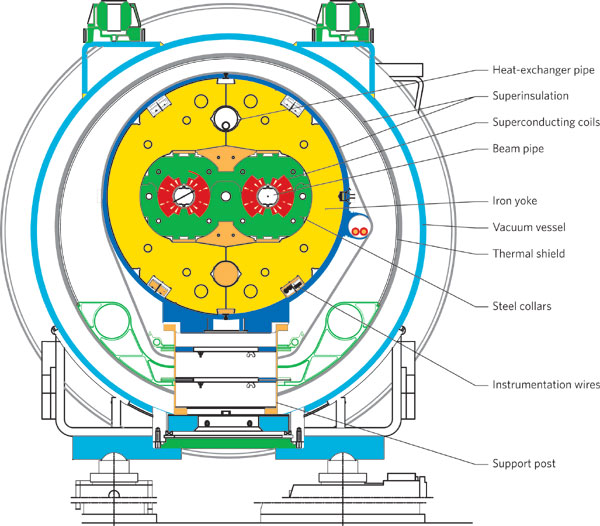
\includegraphics[width=0.65\linewidth]{{LHC_CMS/LHC_Dipole}.jpg}
\caption[A cross section schematic of the LHC Dipole magnet showing the two center beam pipes, superconducting coils (red), and other supporting structures.]{A cross section schematic of the LHC Dipole magnet showing the two center beam pipes, superconducting coils (red), and other supporting structures \cite{Bruning:782076}.}
\label{fig:LHC_Dipole}
\end{center}
\end{figure}

The LHC probes small cross sections by smashing two beams of high energy protons into each-other giving large center of mass energies. In the original design, each proton beam would have $\unit{7}{\TeV}$ of energy giving $\unit{14}{\TeV}$ in the center of mass frame. However, these studies will focus on the early years of LHC operation where the center of mass energies were $\unit{7}{\TeV}$ (2011) and $\unit{8}{\TeV}$ (2012). 

The luminosity of the LHC depends on the geometrical and electrodynamic parameters of the beam. For a beam of particles that are Gaussian distributed, the luminosity is given by the product of the beam current $\left(f_{\text{rev}}n_{b}N_{b}\right)$, brightness $\left(\frac{N_{b}}{\epsilon_{N}}\right)$, energy $\left(\frac{\gamma}{\beta^{*}}\right)$ and a geometric reduction factor $\left(F\right)$:

\begin{equation}
\label{eq:Lumi}
\mathcal{L} = \frac{1}{4\pi}\cdot\left(f_{\text{rev}}n_{b}N_{b}\right)\cdot\frac{N_{b}}{\epsilon_{N}}\cdot\frac{\gamma}{\beta^{*}}\cdot F.
\end{equation}

In this equation \eqref{eq:Lumi} the relevant factors that determine the beam current are the revolution frequency, $\left(f_{\text{rev}}\right)$, the number of proton bunches in each beam, $\left(n_{b}\right)$, and the number of protons in each bunch, $\left(N_{b}\right)$. Generally, the LHC tries to maximize this beam current so that the number of protons in each beam is as large as possible. The brightness of the beam determines how likely two protons are to interact when one bunch crosses another. It is determined by the number of protons in a bunch and the normalized transverse beam emittance, $\left(\epsilon_{n}\right)$, which is a measures of the area of the beam in the position-momentum phase space. The energy of the beam is determined by the relativistic $\gamma$ factor and the value of the beta function at the collision point, $\left(\beta^{*}\right)$. The beta function describes transverse size of the beam and $*$ denotes that this function should be evaluated at the collision point. The final term, $\left(F\right)$, is the geometrical factor that describes the reduction in luminosity because the two beams cross each-other with some non-zero angle between them. 

For the experiments that require the highest luminosities, the LHC was designed to provide $\unit{\power{10}{34}}{\rpsquare{\centi\meter}\reciprocal\second}$. The machine ran at lower luminosities for the first few years of operation as seen in the figures \ref{fig:PeakLumi} \cite{LHC_Lumi}.

\begin{figure}
\begin{center}
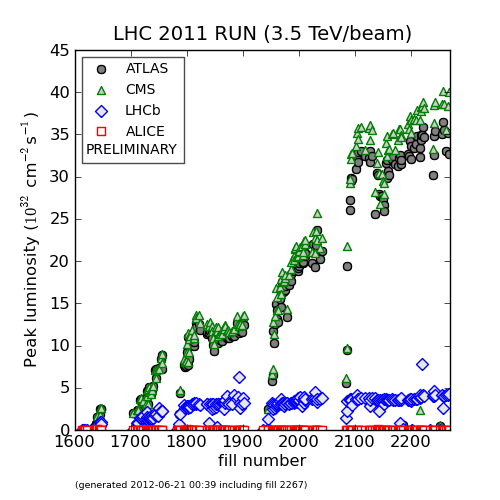
\includegraphics[width=0.45\linewidth]{{LHC_CMS/luminosity_peak_7TeV}.png}
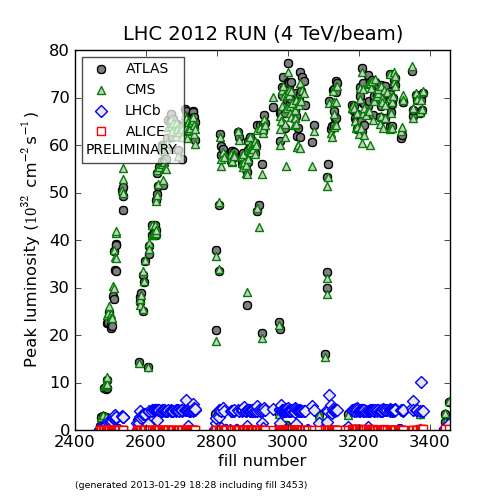
\includegraphics[width=0.45\linewidth]{{LHC_CMS/luminosity_peak_8TeV}.png}
\caption[The peak luminosity delivered to the four main LHC experiments during the 2011 $\unit{7}{\TeV}$ (left) and 2012 $\unit{8}{\TeV}$ (right) runs.]{The peak luminosity delivered to the four main LHC experiments during the 2011 $\unit{7}{\TeV}$ (left) and 2012 $\unit{8}{\TeV}$ (right) runs \cite{LHC_Lumi}.}
\label{fig:PeakLumi}
\end{center}
\end{figure}

To get the protons up to the necessary energies, protons are accelerated through a series of smaller accelerators which are pictured in figure \ref{fig:LHC}. The process starts with the $\unit{50}{\MeV}$ LINAC2 which shoots the protons into a multi-ring booster synchrotron that accelerates them up to $\unit{1.4}{\GeV}$. Next the protons are directed to the Proton Synchrotron (PS) machine which accelerates them up to $\unit{26}{\GeV}$ and generates the bunching and spacing that the LHC uses. To accelerate the beam from $\unit{26}{\GeV}$ up to $\unit{450}{\GeV}$ the beam is fed into the Super Proton Synchrotron (SPS). From the SPS the protons are fed into one of the LHC rings. Before the LHC accelerates these protons up to their final energies, this process is repeated 24 times, 12 to fill each of the two rings. Once the LHC has accelerated these proton bunches to their final energies, the beams are gradually brought together so that they will collide inside the four experiments.

\begin{figure}
\begin{center}
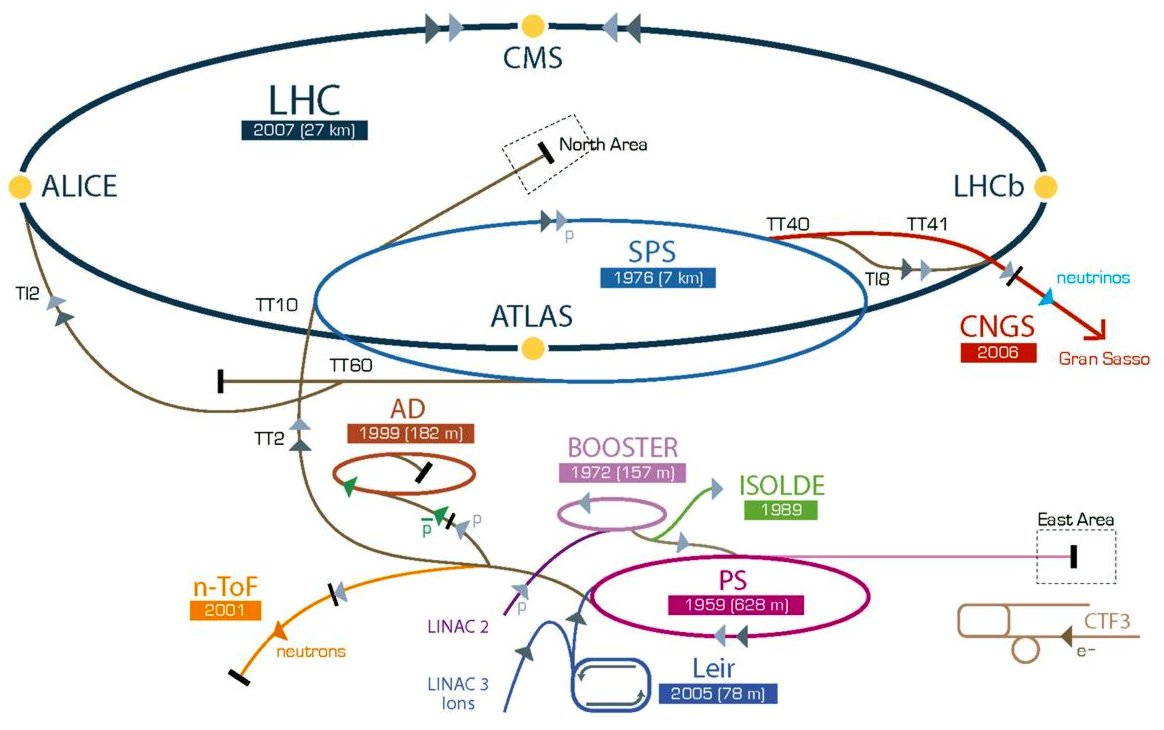
\includegraphics[width=.89\linewidth]{{LHC_CMS/LHC_nature}.jpg}
\caption[This CERN accelerator complex. Showing the full chain of accelerators used for the LHC protons: LINAC2, Booster, PS, SPS, and LHC. Additionally, the four large experiments on the LHC are shown: ALICE, ATLAS, CMS, LHCb.]{This CERN accelerator complex. Showing the full chain of accelerators used for the LHC protons: LINAC2, Booster, PS, SPS, and LHC. Additionally, the four large experiments on the LHC are shown: ALICE, ATLAS, CMS, LHCb \cite{Bruning:2007zzc}.}
\label{fig:LHC}
\end{center}
\end{figure}

The particle physics community built detectors to observe and categorize the particles that are produced when these protons (ions) are collided with each-other. Currently there are four experiments at the LHC: A Toroidal LHC ApparatuS (ATLAS), the Compact Muon Solenoid (CMS), A Large Ion Collider Experiment (ALICE), and Large Hadron Collider beauty (LHCb). The ATLAS and CMS detectors are high luminosity, multi-purpose detectors designed to test many different aspects of the SM, including the Higgs boson. LHCb looks specifically at bottom (beauty) quark interactions, while ALICE is designed for ion collisions. This work took place at the CMS experiment, described in the next sections.

\section{The Compact Muon Solenoid (CMS)}
\label{sec:CMS}

The Compact Muon Solenoid (CMS) experiment is one of the two largest experiments on the LHC. The general goal of the CMS experiment is to collect and study as many interesting events from LHC collisions as possible. To do this, CMS must identify interesting physics events and reconstruct these events as accurately as possible. At the designed energy and luminosity the LHC is expected to create $\sim 1$ billion collision events per second. It would not be possible to reconstruct all of these events, so CMS has an extensive online event selection process, called the `Trigger', that reduces this to about $100$ events per second. Some details of this process are presented in section \ref{sec:TriggerANDreconstruction}, but we will first have a discussion of the different CMS subdetectors.


To quantify how much data CMS has collected we use \textit{integrated luminosity}, which is the time integral of the luminosity, $\int \mathcal{L} dt$. This value tells experimenters how many events to expect for the specific processes they study, $N = \sigma \cdot \int \mathcal{L} dt$, and allows them to test smaller and smaller cross sections. Over the 2011 and 2012 runs\footnote{A run is a period of time denoting specific conditions for the detector or LHC.} of the CMS detector collected $\unit{5.1}{\invfb}$ and $\unit{19.7}{\invfb}$ of integrated luminosity respectively, shown in figure \ref{fig:CMSLumi}.

\begin{figure}
\begin{center}
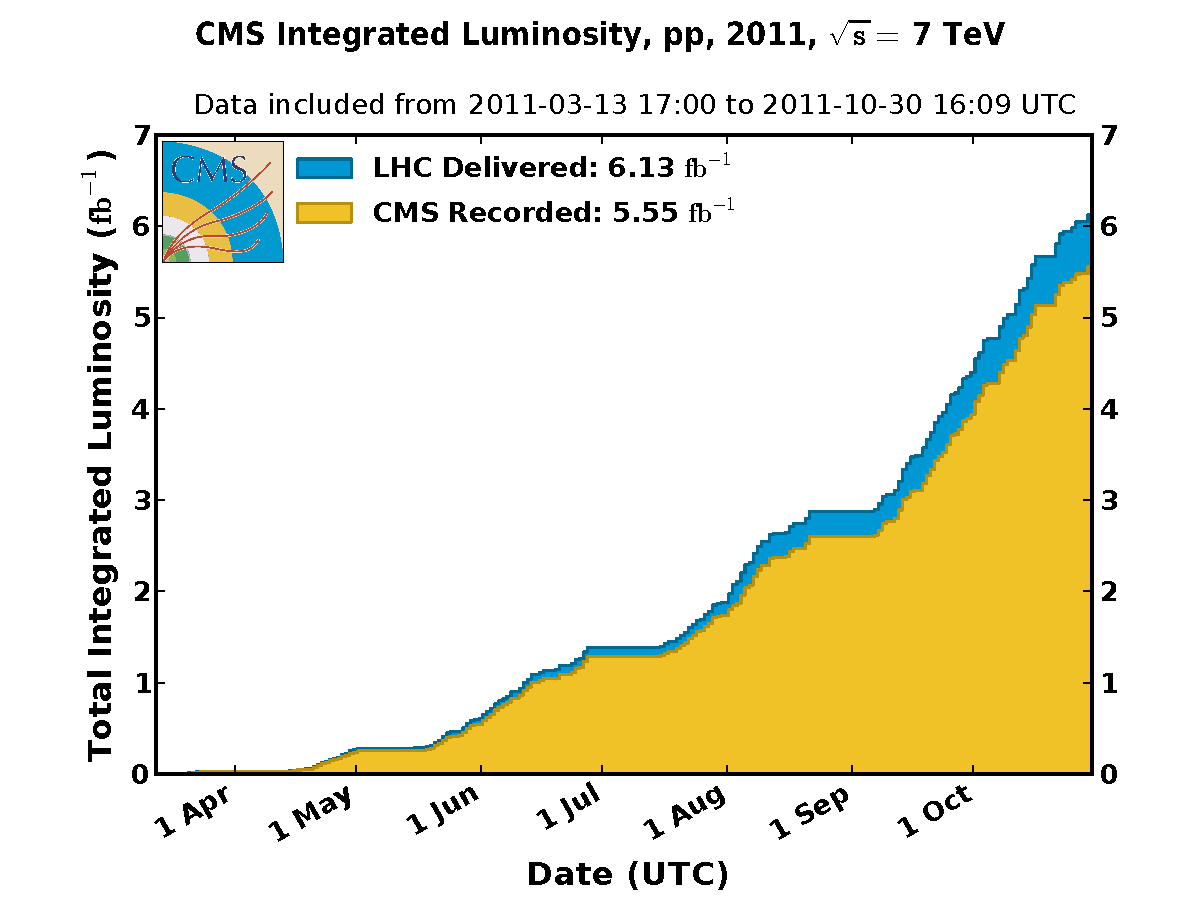
\includegraphics[width=0.45\linewidth]{{LHC_CMS/luminosity_int_7TeV}.pdf}
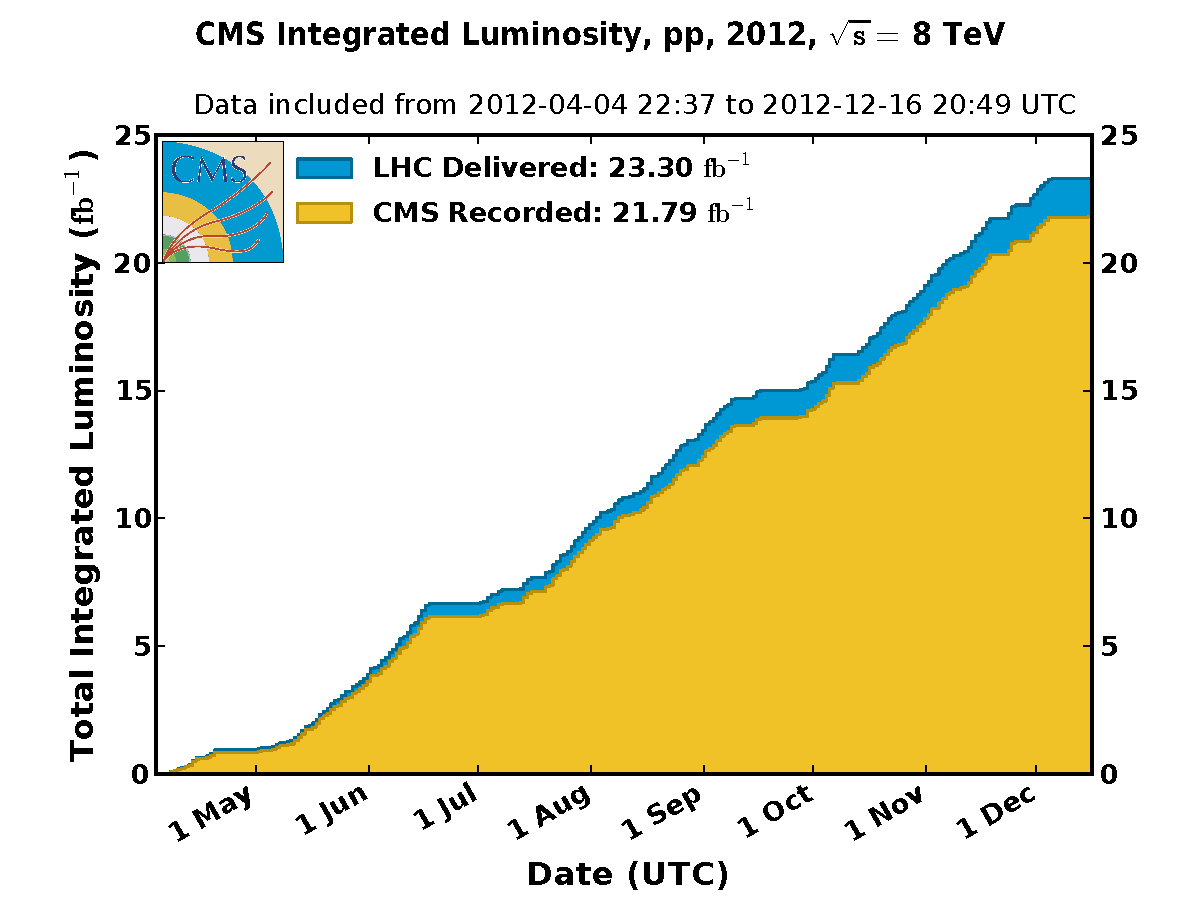
\includegraphics[width=0.45\linewidth]{{LHC_CMS/luminosity_int_8TeV}.pdf}
\caption[The integrated luminosity delivered and collected by the CMS experiment during the 2011 $\unit{7}{\TeV}$ (left) and 2012 $\unit{8}{\TeV}$ (right) runs.]{The integrated luminosity delivered and collected by the CMS experiment during the 2011 $\unit{7}{\TeV}$ (left) and 2012 $\unit{8}{\TeV}$ (right) runs, \cite{CMS_Lumi}.}
\label{fig:CMSLumi}
\end{center}
\end{figure}

To maximize the physics results that can be pulled from this data, CMS was designed with key features that give credence to its name. While it may seem oxymoronic to call a $\unit{21.6}{m}$ long and $\unit{15}{m}$ in diameter experiment `compact', the name is fitting because it is designed to put the sub-detectors within CMS close together. This compact design is a result of the $\unit{4}{\tesla}$ magnetic field that is the heart of the CMS detector. The Magnet, discussed more in section \ref{sec:Magnet}, causes the charged particles generated in collisions to bend as the flow out from the interaction point so identifying particles and measuring their momentum requires detectors that are close together. Working in concert with this field, the CMS detectors are designed to fit together as a 'cylindrical onion'. The layers of detectors and sub-detectors radiate outward from the point where the protons collisions take place. Each layer is designed to maximize the physics information that can be obtained at different distances from these collisions. The majority of the information in this section follows \cite{Bayatian:922757}.

\begin{figure}
\begin{center}
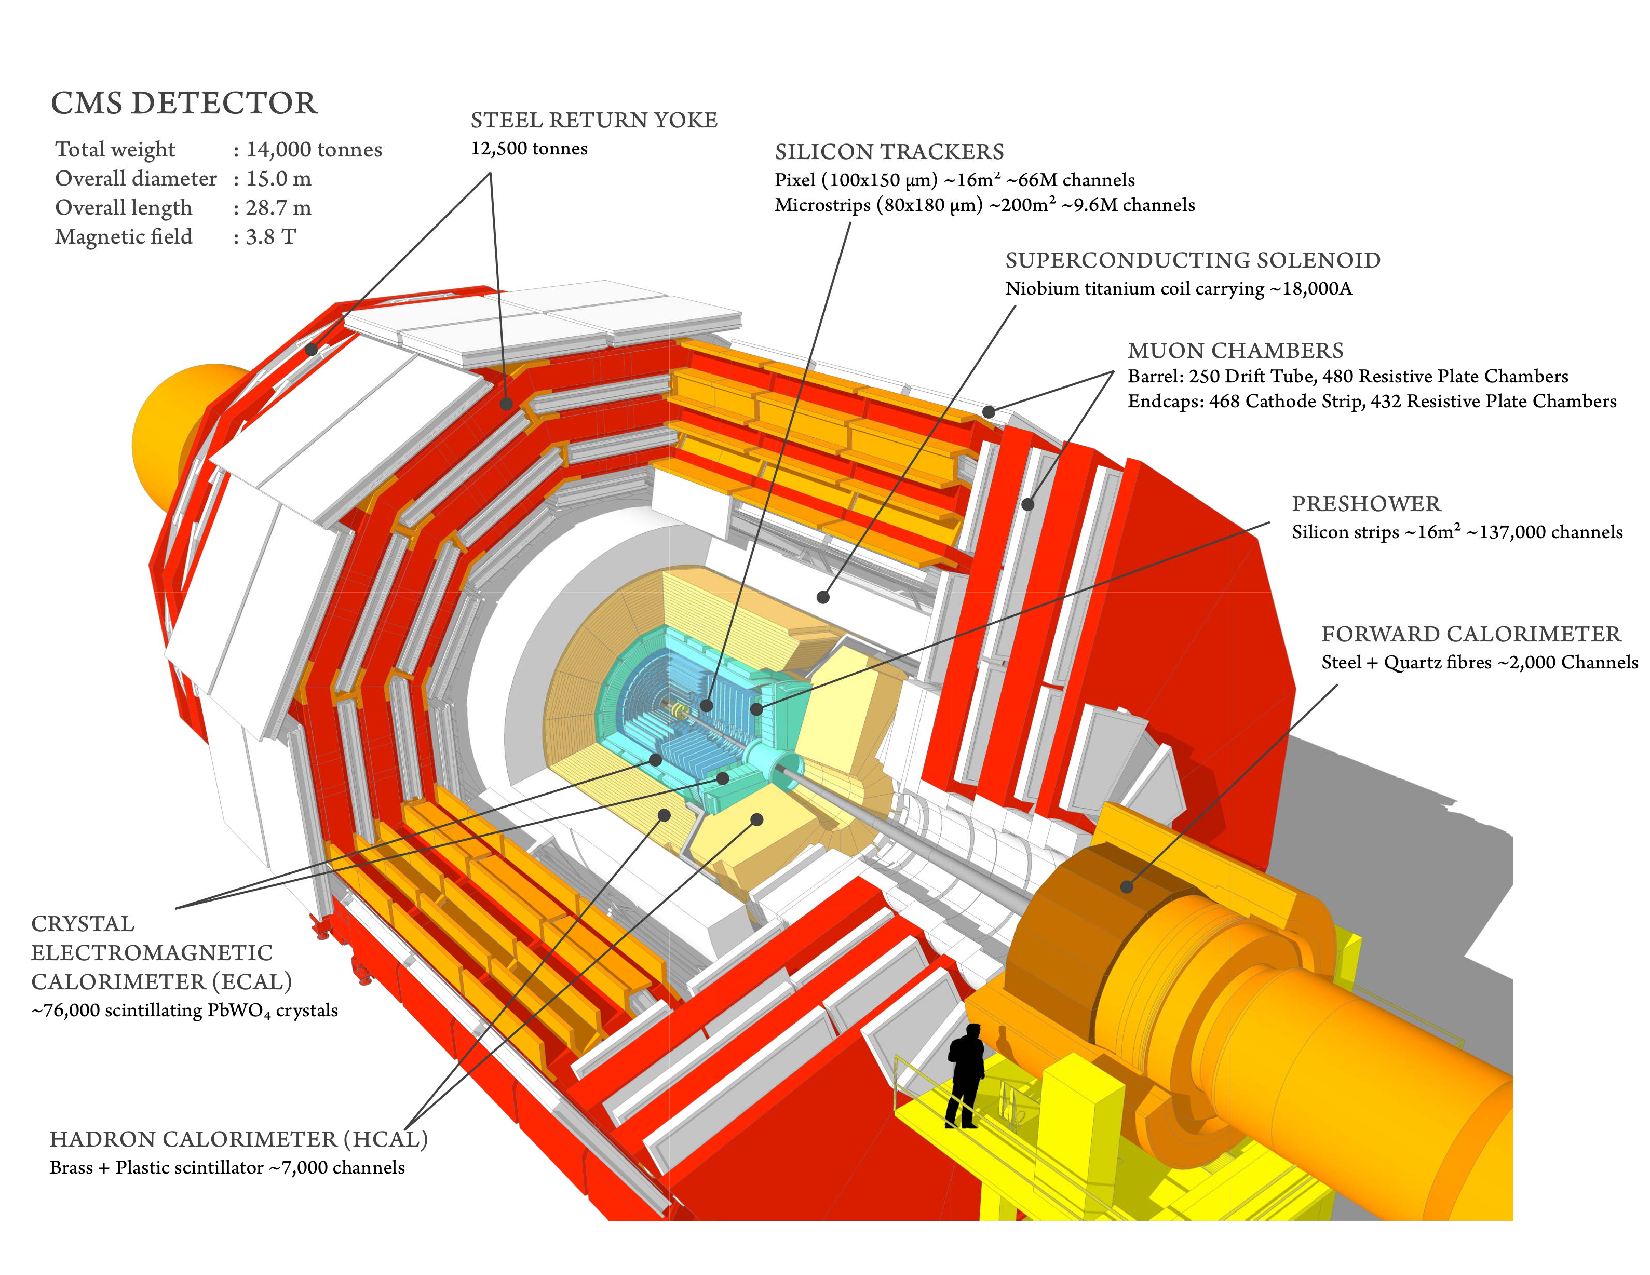
\includegraphics[width=.89\linewidth]{{LHC_CMS/cms_onion}.png}
\caption[Sectional view of the CMS detector. The LHC beams travel in opposite directions along the central axis of the CMS cylinder colliding in the middle of the CMS detector.]{Sectional view of the CMS detector. The LHC beams travel in opposite directions along the central axis of the CMS cylinder colliding in the middle of the CMS detector \cite{Sakuma:2013jqa}.}
\label{fig:CMS_onion}
\end{center}
\end{figure}

A sectional view of the CMS detectors can be seen in figure \ref{fig:CMS_onion}. From this image you can see a summary of the different subdetectors that we discuss from inside out. The innermost detector is the Silicon tracker, discussed in section \ref{sec:Tracker}, this detector is designed to give good momentum resolution for charged particles and high reconstruction efficiency requiring precise alignment of the tracking system. Additionally, this tracker needs to be able to efficiently tag $\tau$'s and b's, which will have a displaced vertex due to their long lifetimes. This requires pixel detectors close to the interaction point. 

Just outside of the tracking system is the Electromagnetic calorimeter (ECAL), discussed in section \ref{sec:ECAL}, which gives good energy and mass resolution for photons and electrons and wide geometric coverage. Further, the high segmentation of the system allows for great directional discrimination to determine the origin of the particles and to determine how isolated they are from other particles. 

The final detector that still lies inside the bore of the solenoid is the Hadronic Calorimeter (HCAL), described in section \ref{sec:HCAL}. This detector allows for accurate measurements of quark-jet mass resolution and the lateral segmentation gives directional information that is key to determine any imbalance in the transverse energy of a collision, $E_{T}^{\text{miss}}$.

Outside of the solenoid magnet lies the Muon System, described in section \ref{sec:Muon}, and the large Iron return yokes. This is the largest and heaviest part of the CMS detector\footnote{When combined with the magnet and other subdetectors the full CMS detector weighs $\sim\unit{14,000}{\text{tonnes}}$.}. This system gives good muon identification and good momentum resolution over a wide range of angles and energies for high momentum muons.

As we describe the CMS detector we will need to define a set of spacial coordinates so that we can locate ourselves within the detector. The coordinate system is defined to put the origin at the nominal collision point inside the experiment, the y-axis pointing vertically upward, the x-axis pointing along the radius of the LHC, and the z-axis pointing along the beam direction. The geometry of the detector is already cylindrical, so a modified form of cylindrical units are use for most studies. The azimuthal angle $\phi$, is given by the angle from the x-axis in the x-y plane. The polar angle, $\theta$ (from the z-axis), normally used in cylindrical coordinates, is replaced by the pseudorapidity, $\eta = -\ln\tan\left(\theta/2\right)$. The z-axis is the same as the cartesian definition. Often, interesting physics events will show distinct features in the momentum or energy transverse to the beam direction, $p_{T}$ and $E_{T}$ respectively.
 
\subsection{The Magnet}
\label{sec:Magnet}

The defining feature of CMS is the superconducting solenoid magnet, the parameters are given in table \ref{tab:CMSmagnet}. The large bending power that CMS is designed for is obtained form a reasonably-sized superconducting solenoid where the bending for charged particles starts at the primary vertex. The strong field is needed to give good momentum resolution. It bends muons tightly so that the charge is unambiguous and giving a momentum resolution of $\Delta p / p \sim 10\%$ at $p = \unit{1}{\TeVoverc}$. This design also leads to a reasonable field in the forward region where many of the detected particles will be.

\bgroup
\renewcommand{\arraystretch}{0.5}% Tighter
\begin{table}
\begin{center}
\begin{tabular}{| l | c |}
\hline 
Field & $\unit{4}{\tesla}$ \\ 
\hline 
Inner Bore & $\unit{5.9}{\meter}$ \\ 
\hline 
Length & $\unit{12.9}{\meter}$ \\ 
\hline 
Number of Turns & 2168 \\ 
\hline 
Current & $\unit{19.5}{\kilo\ampere}$ \\ 
\hline 
Stored Energy & $\unit{2.7}{\giga\joule}$ \\ 
\hline 
Hoop stress & $\unit{64}{\text{atm}}$ \\ 
\hline 
\end{tabular}
\end{center}
\caption[Parameters of the CMS superconducting solenoid.]{Parameters of the CMS superconducting solenoid, \cite{Bayatian:922757}.}
\label{tab:CMSmagnet}
\end{table}
\egroup

The magnet itself is constructed from high-purity aluminum-stabilized conductor and is indirectly cooled using a thermosiphon method.  While this type of magnet has been used at other experiments, it was a large step up in many aspects from previous magnets. To create a solenoid with the field and dimensions, a four-layer conductive winding with a large diameter wire was used so it could withstand the large outward pressure (hoop stress). The conductor carries  a $\unit{19.5}{\kilo\ampere}$ current and is co-extruded with pure and alloy aluminum to stabilize it thermally and mechanically. The conductor was manufactured in twenty continuous lengths, each of $\unit{2.65}{\kilo\meter}$. Four of these lengths were used to make each of the five coil modules within the magnet.

\begin{figure}
  \begin{center}
    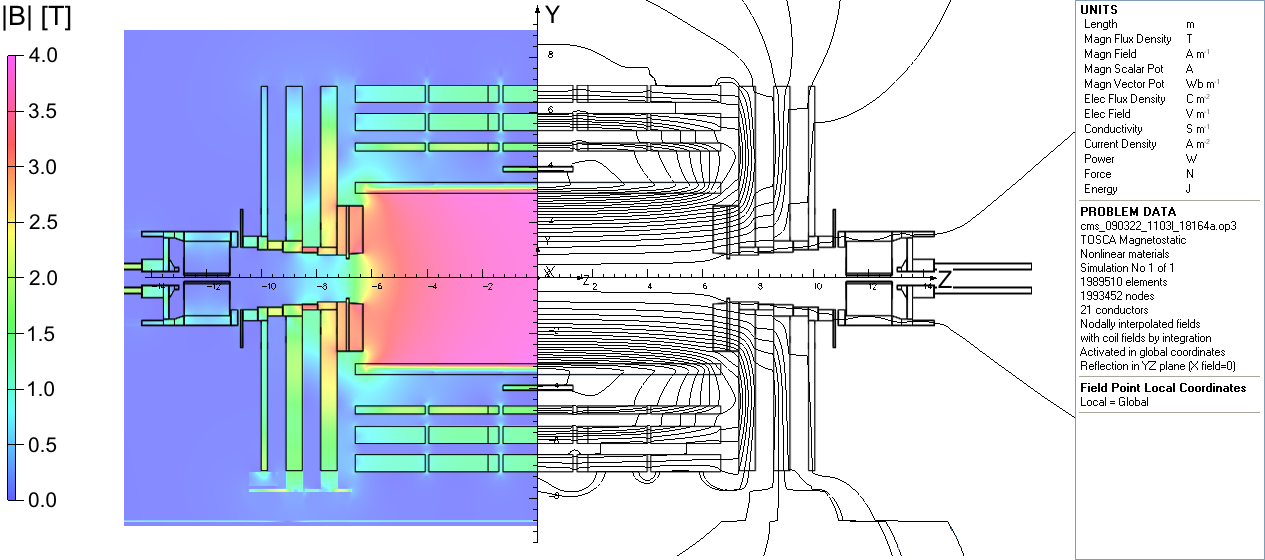
\includegraphics[width=\textwidth,trim=0 0 193 0, clip]{LHC_CMS/lines_6wb3_4_nologo.png}

    \caption[Value of magnetic field $|B|$ (left) and field lines (right) predicted on
      a longitudinal section of the CMS detector, for the underground
      model at a central magnetic flux density of 3.8~T. Each field
      line represents a magnetic flux increment of 6~Wb.]{Value of magnetic field $|B|$ (left) and field lines (right) predicted on
      a longitudinal section of the CMS detector, for the underground
      model at a central magnetic flux density of 3.8~T. Each field
      line represents a magnetic flux increment of 6~Wb \cite{Chatrchyan:2009si}.}
    \label{fig:FieldLines}
  \end{center}
\end{figure}

Working in concert with the magnet is the iron return yoke of the muon system. As can be seen in figure \ref{fig:FieldLines}, the superconducting magnet generates a large magnetic field inside the solenoid while the return flux of the field concentrates itself in the large iron structures that house the different muon detectors. These performance predictions were later confirmed by both monitors installed in the detector and with data collected from cosmic rays \cite{Chatrchyan:2009si}.

\subsection{The Inner Tracker System}
\label{sec:Tracker}

The inner tracker system is the first detector that a particle generated from an LHC collision will encounter. At the LHC, determining the origin of these particles is key and made more difficult due to the small gaps between proton bunches. The spatial resolution of the silicon tracker detector allows a particle to be mapped to the primary collision vertex (\textit{primary vertex}), secondary vertices, or identify them as \textit{pileup events}. At the designed luminosity, the LHC is expected to generate about 20 collisions\footnote{We expect more moving forward.} that will all be superimposed on an event of interest. This means that $\sim{1000}$ charged particles will appear in the detector for every interesting event. The job of the inner tracker is to measure the charge and momentum of these particles, and determine which of these originate from what vertex. To do this, the tracker has two distinct types of detectors; the 66 million \textit{silicon pixels} and 9.6 million \textit{silicon strips}. It is also vital that the positions of these detectors is accurately known at all times so that the system can operate at its ideal level. The process of determining the positions of these detectors is called \textit{Tracker Alignment} and an overview of work performed for this task is presented.

\begin{figure*}[hbtp]
  \begin{center}
    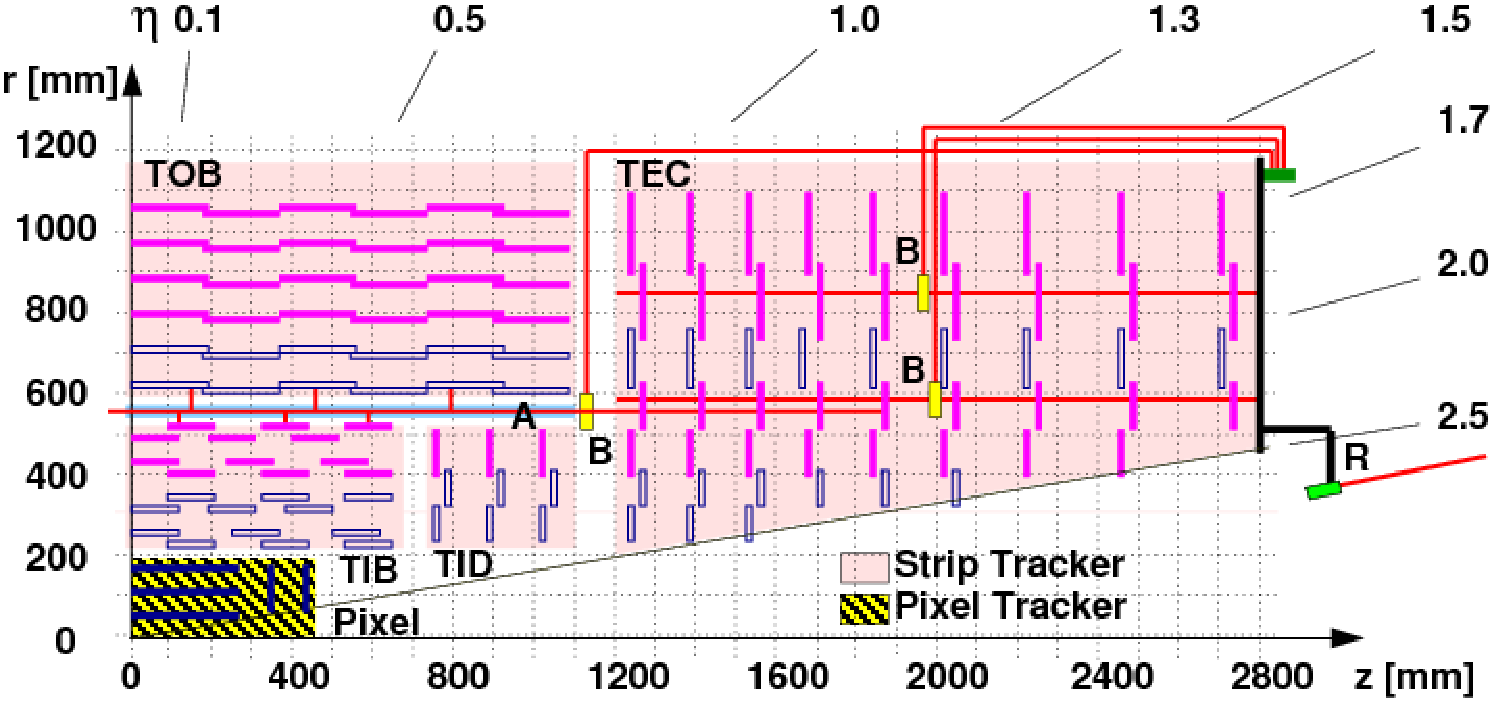
\includegraphics[width=0.7\textwidth]{{LHC_CMS/TrackerLayoutWithLAS}.pdf}
    \caption[Schematic view of one quarter of the silicon tracker in the $r$--$z$ plane.
      The positions of the pixel modules are indicated within the hatched area. At
      larger radii within the lightly shaded areas, solid rectangles represent single
      strip modules, while hollow rectangles indicate pairs of strip
      modules mounted back-to-back with a relative stereo angle.]{Schematic view of one quarter of the silicon tracker in the $r$--$z$ plane.
      The positions of the pixel modules are indicated within the hatched area. At
      larger radii within the lightly shaded areas, solid rectangles represent single
      strip modules, while hollow rectangles indicate pairs of strip
      modules mounted back-to-back with a relative stereo angle \cite{Chatrchyan:2014wfa}.}
    \label{fig:TrackerLayout}
  \end{center}
\end{figure*}

\subsubsection{Pixel Tracker}
\label{sec:Pixel}

Close to the interaction vertex the tracker consists of three layers of silicon pixel modules in the barrel region and two layers of silicon pixel modules in each forward region. The layout of the pixel detector is shown in figure \ref{fig:PixelHardware}. Each of the three barrel layers are located at radii $\unit{4.4}{\centi\meter}$, $\unit{7.3}{\centi\meter}$, and $\unit{10.2}{\centi\meter}$ from the nominal interaction point and each is $\unit{53}{\centi\meter}$ long. On either side of the three barrel layers are two end disks placed at $\abs{z} = \unit{34.5}{\centi\meter}$ and $\unit{46.5}{\centi\meter}$. 

\begin{figure}
\begin{center}
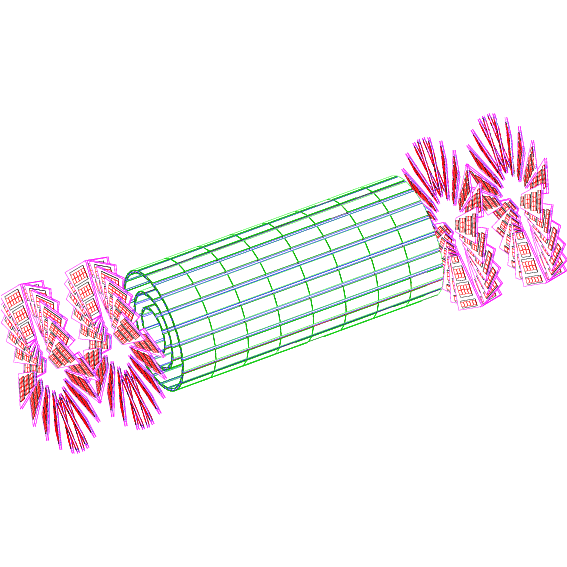
\includegraphics[width=.45\linewidth]{{LHC_CMS/PixelHardware}.pdf}
\caption[Layout of the pixel detectors in the CMS tracker.]{Layout of the pixel detectors in the CMS tracker \cite{Bayatian:922757}.}
\label{fig:PixelHardware}
\end{center}
\end{figure}

All of the pixel modules start from the same base array ($\unit{52}{\text{column}} \times \unit{80}{\text{row}}$) of pixels (size: $\unit{100}{\micro\meter} \times \unit{150}{\micro\meter}$) bump-bonded to a readout chip (ROC). Each pixel is connected to its own amplifier, shaper,  and comparator (including an individual 3-bit DAC threshold) which is connected to a `double-column' group shown in figure \ref{fig:Pixel_ROC}. The periphery of each double-column contains a data buffer, timestamp, and corresponding control and readout electronics. ROC's are grouped into modules. Each module has a different number of ROCs depending on the geometry of the region where the detectors are placed. 

\begin{figure}
\begin{center}
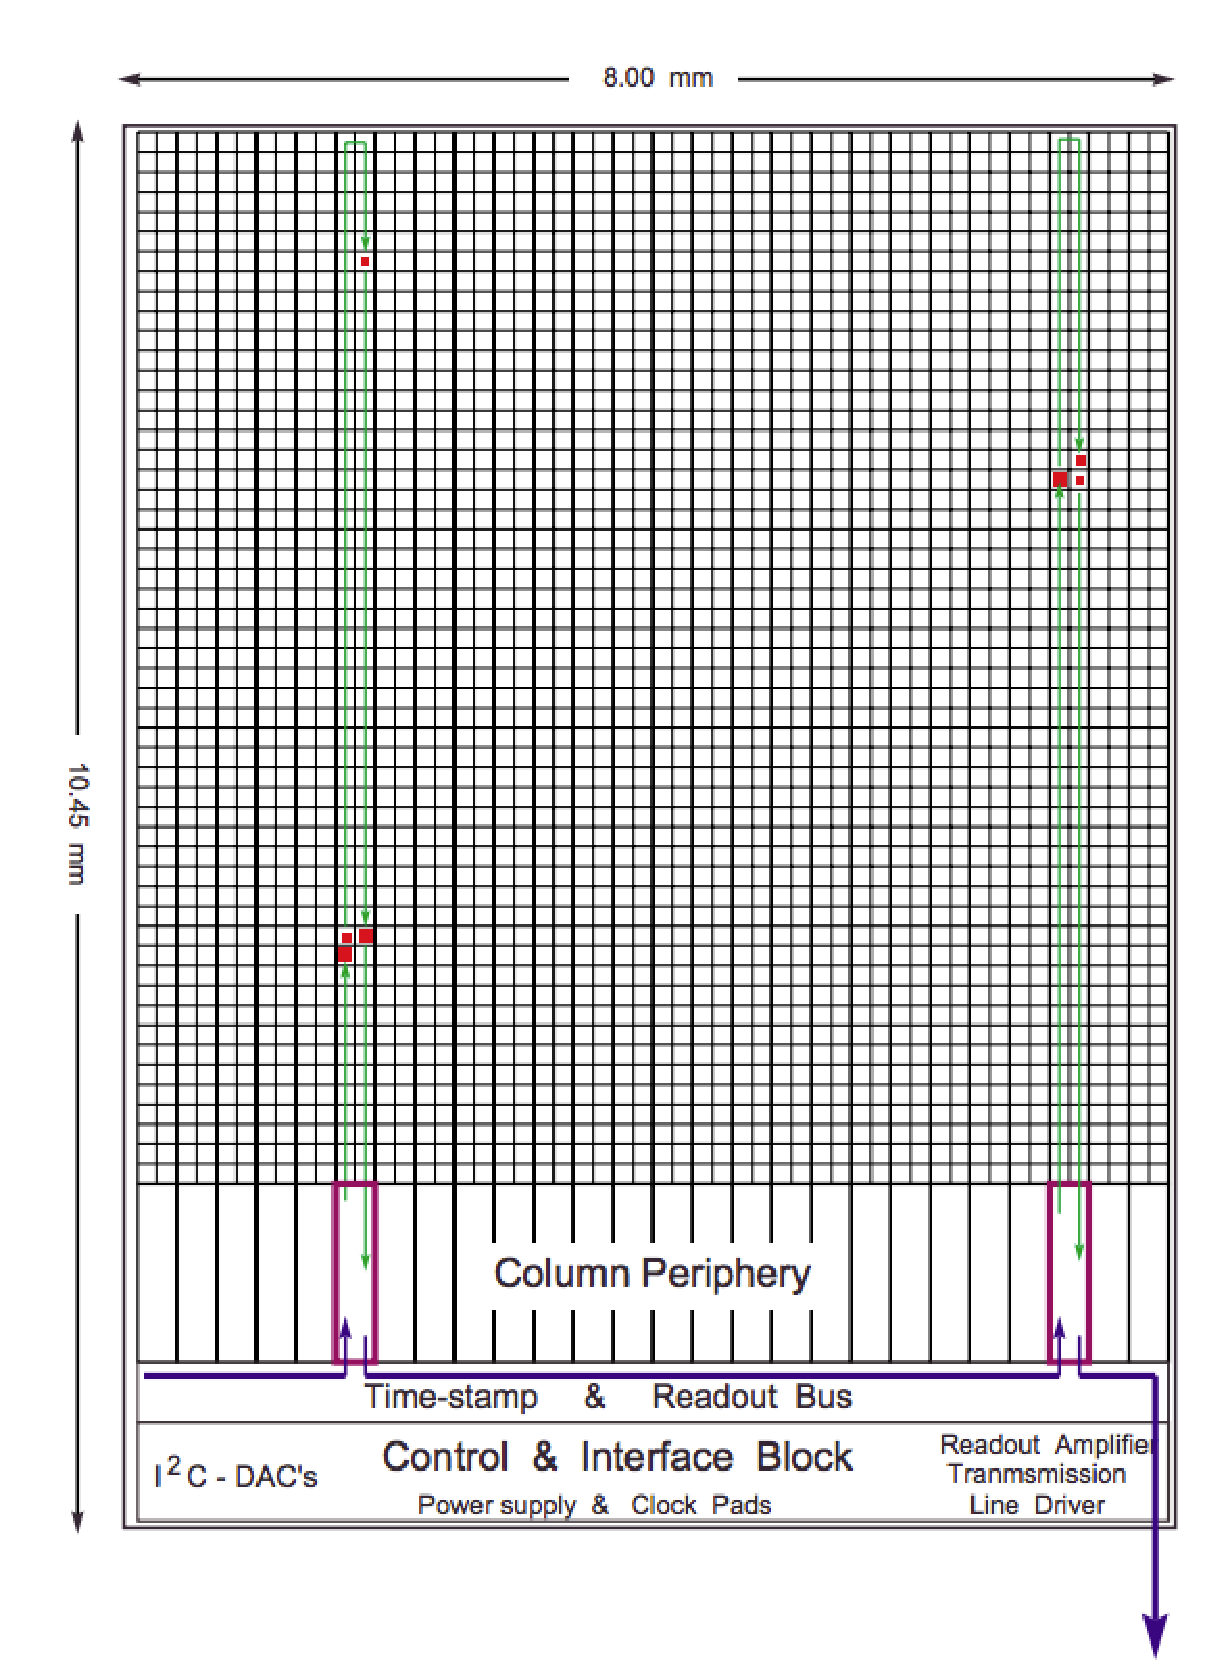
\includegraphics[width=.45\linewidth]{{LHC_CMS/Pixel_ROC}.pdf}
\caption[Layout of the pixel sensor in the CMS tracker.]{Layout of the pixel sensor in the CMS tracker \cite{Kotlinski:478252}.}
\label{fig:Pixel_ROC}
\end{center}
\end{figure}

The pixel barrel (BPIX) contains 768 modules grouped into three layers\footnote{There are smaller substructures within each layer.} and two \textit{half-barrels}\footnote{All three layers together make one half-barrel.}. While the forward pixel detectors (FPIX) are made from 672 modules grouped into two layers of turbine-like blades. The forward structures are also grouped into \textit{half-cylinders} similar to the barrel region\footnote{Again, the two layers together make the half-cylinders.}. Both the barrel layers and the blades are oriented to benefit form the large Lorentz effect (charge drift in a magnetic field) that increases the resolution through charge sharing between the pixels.

In the end, the inner tracker comprises 66 million individual pixel channels readout using approximately 16000 ROCs, giving a spatial resolution of about $\sim\unit{10}{\micro\meter}$ in $r$-$\phi$ and $\unit{20}{\micro\meter}$ in $z$. This high resolution allows for precise momentum determination for particles as they curl in the high magnetic field. It is also key to determining the origin of the particles that CMS measures. The $\sim \unit{1}{\power{\meter}{2}}$ silicon pixel detector provides coverage up to $\abs{\eta} < 2.4$.


\subsubsection{Strip Tracker}
\label{sec:Strip}

Much larger than the  pixel tracker is the $\sim \unit{200}{\power{\meter}{2}}$ silicon strip tracker. The strip tracker is divided into four parts: TIB (tracker inner barrel), TID (tracker inner disks),  TOB (tracker outer barrel), and TEC (tracker end cap). The CMS tracker is the largest silicon detector ever built. Different regions of the strip tracking system have different module types summarized in table \ref{tab:Strips}. All together, the Silicon Strip Tracker has complete coverage up to $\abs{\eta} < 2.4$.

\bgroup
\renewcommand{\arraystretch}{0.5}% Tighter
\begin{table}
\begin{center}
\begin{tabular}{ l | r | r | r }
\hline 
part & No. detectors & thickness $\left(\micro\meter\right)$ & mean pitch $\left(\micro\meter\right)$\\ 
\hline 
TIB & 2724 & 320 & 81/118 \\
TOB & 5208 & 500 & 81/183 \\
TID & 816 & 320 & 97/128/143 \\
TEC(inner) & 2512 & 320 & 96/126/128/143 \\
TEC(outer) & 3888 & 500 & 143/158/183 \\
\hline 
\end{tabular}
\end{center}
\caption[Detector types in the silicon strip tracker.]{Detector types in the silicon strip tracker, \cite{Bayatian:922757}.}
\label{tab:Strips}
\end{table}
\egroup

In the barrel region the coverage for the TIB and TOB is very different. The TIB has four layers and covers $\abs{z} < \unit{65}{\centi\meter}$ with silicon sensor of a thickness of $\unit{320}{\micro\meter}$. The first two layers are made with ``stereo" modules in order to provide both $r$-$\phi$ and $r$-$z$ measurements. These stereo modules are made with a stereo angle of $\unit{100}{\milli\radian}$ giving the TIB single-point resolution of $23$-$\unit{34}{\micro\meter}$ in $r$-$\phi$ and $\unit{23}{\micro\meter}$ in $z$. The TOB has six layers covering $\abs{z} < \unit{110}{\centi\meter}$ with silicon sensor of a thickness of $\unit{500}{\micro\meter}$. The first two layers of the TOB are also stereo modules with a stereo angle of $\unit{100}{\milli\radian}$. This gives the whole TOB a resolution of $35$-$\unit{52}{\micro\meter}$ in $r$-$\phi$ and $\unit{52}{\micro\meter}$ in $z$.

The each of the two TECs comprises nine disks that cover the $\unit{120}{\centi\meter} < \abs{z} < \unit{280}{\centi\meter}$ forward region. While the TID covers the gap between the TIB and the TEC. Both the TID and TEC modules are arranged in rings centered at the beam line. The strips in these sensors radiate outward from the beam line so the pitch is different for each strip. The first two rings of the TID and the first, second, and fifth rings of the TEC are stereo modules as well allowing for more precise resolution. The TID and first three rings for the TEC have $\unit{320}{\micro\meter}$ sensors while the rest of the TEC has $\unit{500}{\micro\meter}$ sensors.

All of these structures (BPIX, FPIX, TIB, TOB, TID, TEC) are mounted in carbon-fiber structures and are cooled to ensure they operate correctly for a long time\footnote{Because of technical problems during run 1 the detectors were not kept as cold as originally designed.}. Using the precise position information that the tracker provides CMS is able to determine with very high confidence the momentum and impact parameter (How close a particle's path is the the origin.) of particles, see figure \ref{fig:TrackerResolution}. Careful consideration is taken when these detectors are moved and installed but precise determination of the exact location of all components is key to keep the optimal resolution of these detectors. This process is not only vital during the LHC startup but care needs to be taken as the detector takes data to ensure no loss in performance.

\begin{figure}
\begin{center}
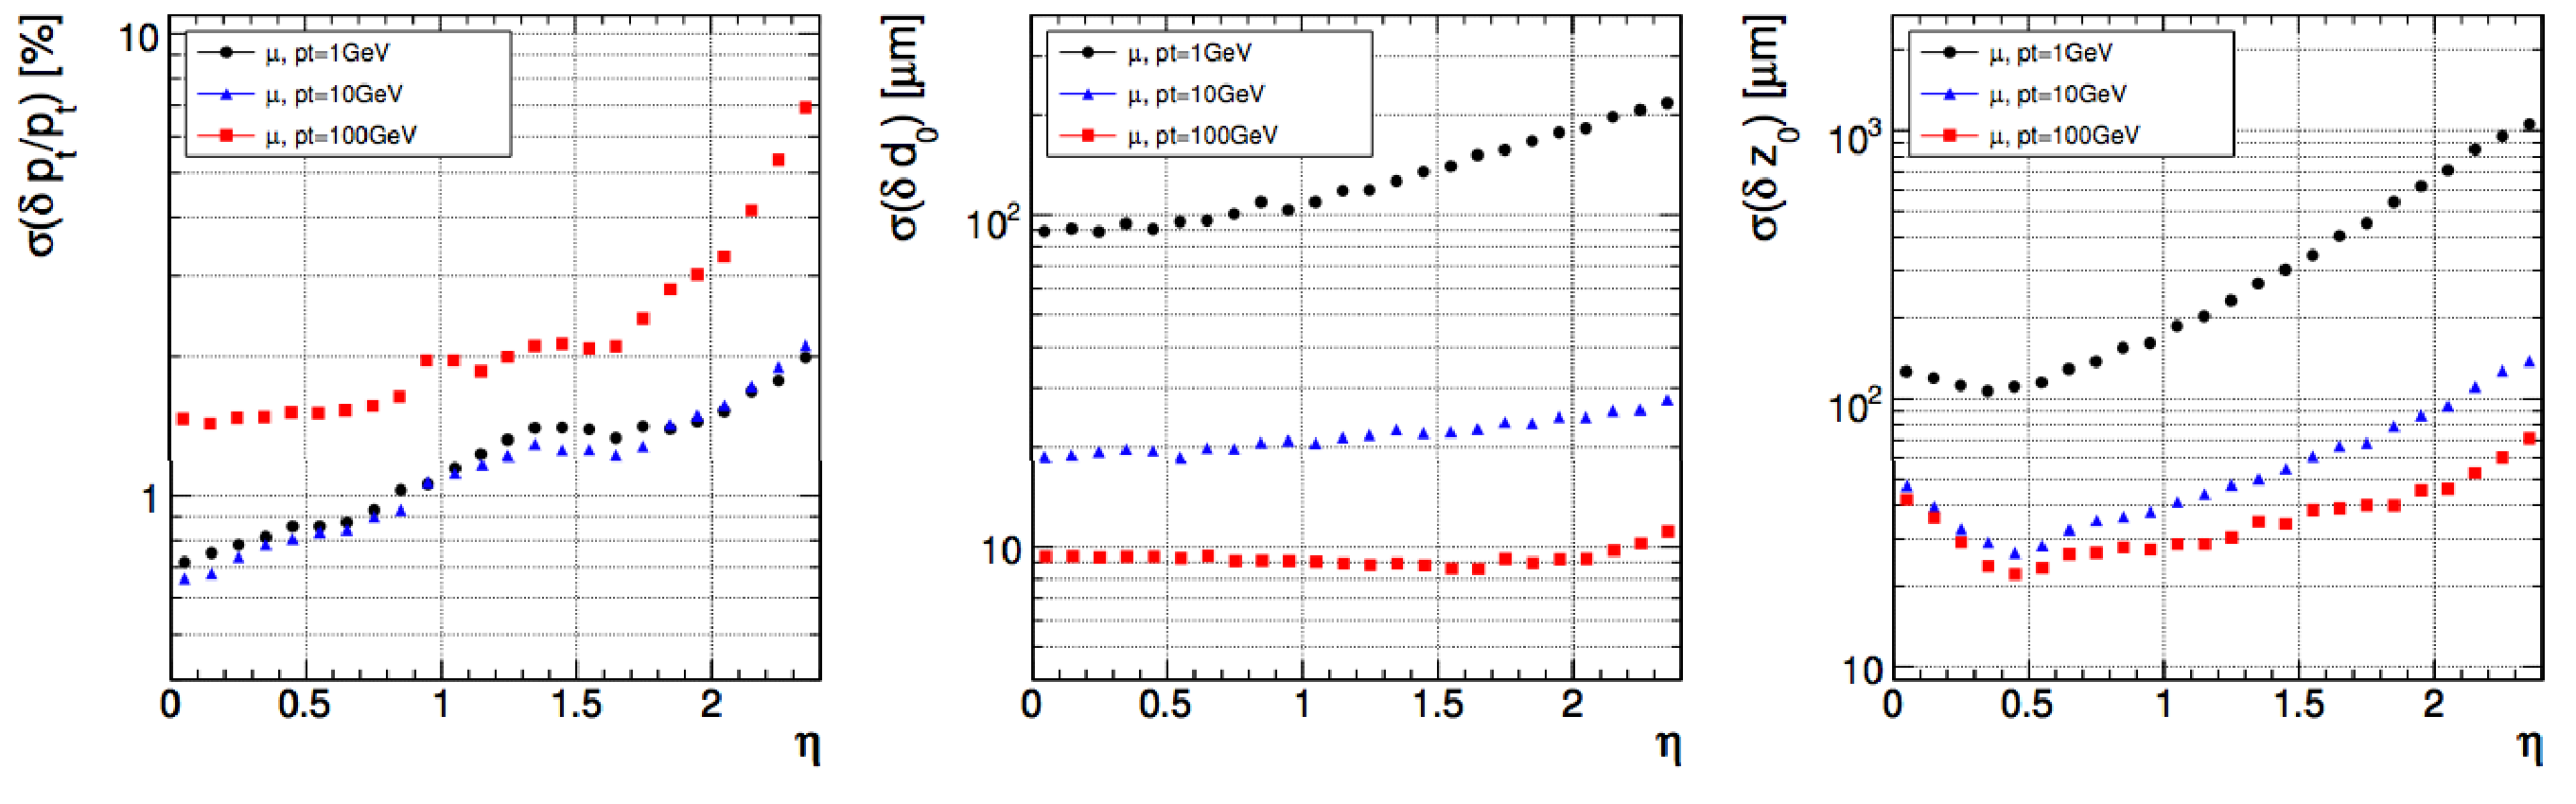
\includegraphics[width=.95\linewidth]{{LHC_CMS/TrackerResolution}.pdf}
\caption[Predicted resolution of several track parameters for single muons with $1$, $10$, and $\unit{100}{\GeV}$: transverse momentum (left), transverse impact parameter (center), and longitudinal impact parameter (right).]{Predicted resolution of several track parameters for single muons with $1$, $10$, and $\unit{100}{\GeV}$: transverse momentum (left), transverse impact parameter (center), and longitudinal impact parameter (right). \cite{Chatrchyan:1129810}.}
\label{fig:TrackerResolution}
\end{center}
\end{figure}

\subsection{Electromagnetic Calorimeter}
\label{sec:ECAL}

The CMS Electromagnetic Calorimeter (ECAL) is composed of $61200$ lead tungstate $\left(\mathrm{PbWO_{4}}\right)$ crystals mounted in the barrel part of the detector and $7324$ crystals in each of the two end caps. Together the barrel and end caps make a homogeneous and hermetic scintillating layer surrounding the Inner Tracker. The crystals were chosen to have short radiation and Moliere lengths while being fast radiation hard scintillators. Due to the low light yield of the crystal, silicon avalanche photo diodes (barrel) or vacuum phototriodes (end cap) are used because they can operate in the magnetic field. Additionally, to stabilize the response of the crystals and photo diodes a cooling system is used to maintain temperature stability. Thus, the ECAL is a compact calorimeter that is fast, has fine granularity, and is radiation resistant.

\begin{figure}
\begin{center}
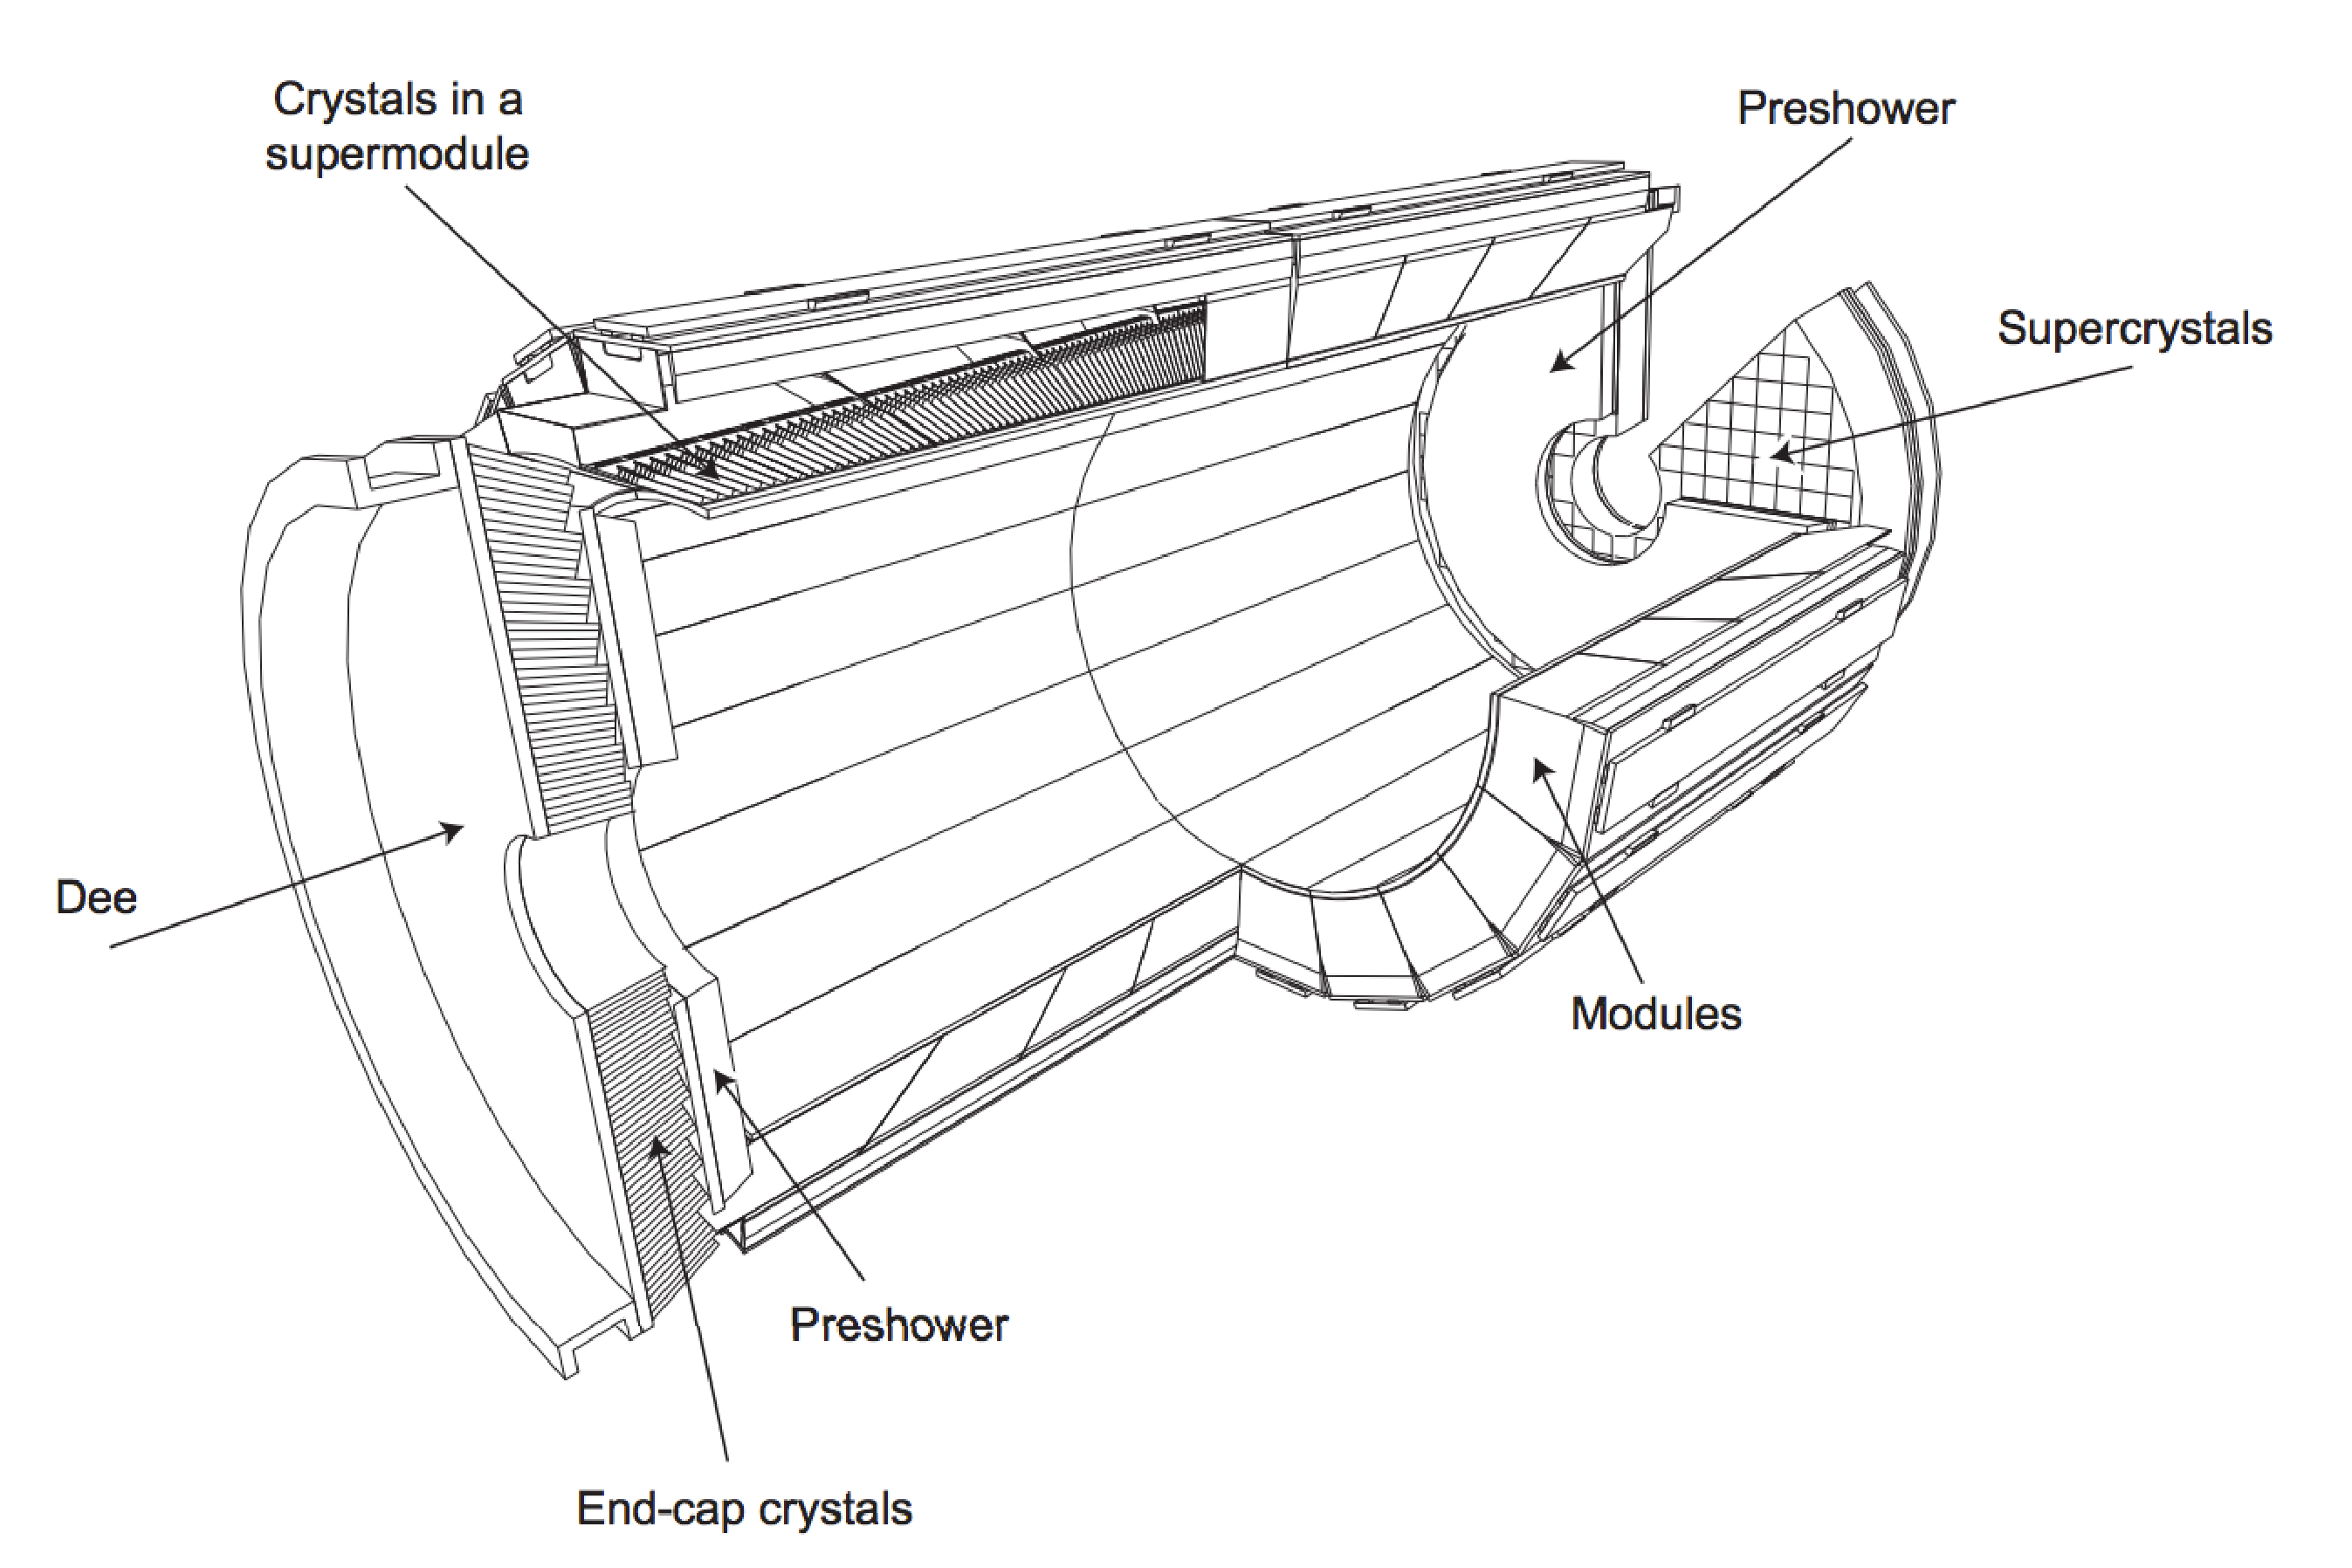
\includegraphics[width=.95\linewidth]{{LHC_CMS/CMSecal}.pdf}
\caption[Layout of the CMS electromagnetic calorimeter showing the arrangement of crystal modules, supermodules and end caps, with the preshower in front.]{Layout of the CMS electromagnetic calorimeter showing the arrangement of crystal modules, supermodules and end caps, with the preshower in front. \cite{Chatrchyan:1129810}.}
\label{fig:CMSecal}
\end{center}
\end{figure}

The ECAL barrel section (EB) has an inner radius of $\unit{129}{\centi\meter}$ and constructed as 36 identical ``supermodules" each covering half the barrel length and covering a range of $0 < \abs{\eta} < 1.479$. The crystals are installed to be quasi-projective (axis tilted $\unit{3}{\degree}$) to the nominal vertex arranged in an $\eta$-$\phi$ grid. They have a front face cross-section of $22\times\unit{22}{\power{\meter}{2}}$ and a length of $\unit{230}{\milli\meter}$.

The ECAL end caps (EE) lie at a distance of $\unit{314}{\centi\meter}$ from the vertex and cover a range of  $1.479 < \abs{\eta} < 3.0$. The end cap crystals, like the barrel, are off-point from the nominal vertex but are arranged in an $x$-$y$ grid. They have a larger face size than the barrel crystals, $28.6\times\unit{28.6}{\power{\meter}{2}}$ and a length of $\unit{220}{\milli\meter}$. Additionally, a preshower detector is placed in front of the EE consisting of two planes of silicon strip detectors each placed behind a layer of lead absorber disks. 

While the specifics of particle reconstruction are discussed in section \ref{sec:TriggerANDreconstruction}, figure \ref{fig:ECALresolution} shows the electron resolution of the EB system compared to and then combined with the inner tracker system.

\begin{figure}
\begin{center}
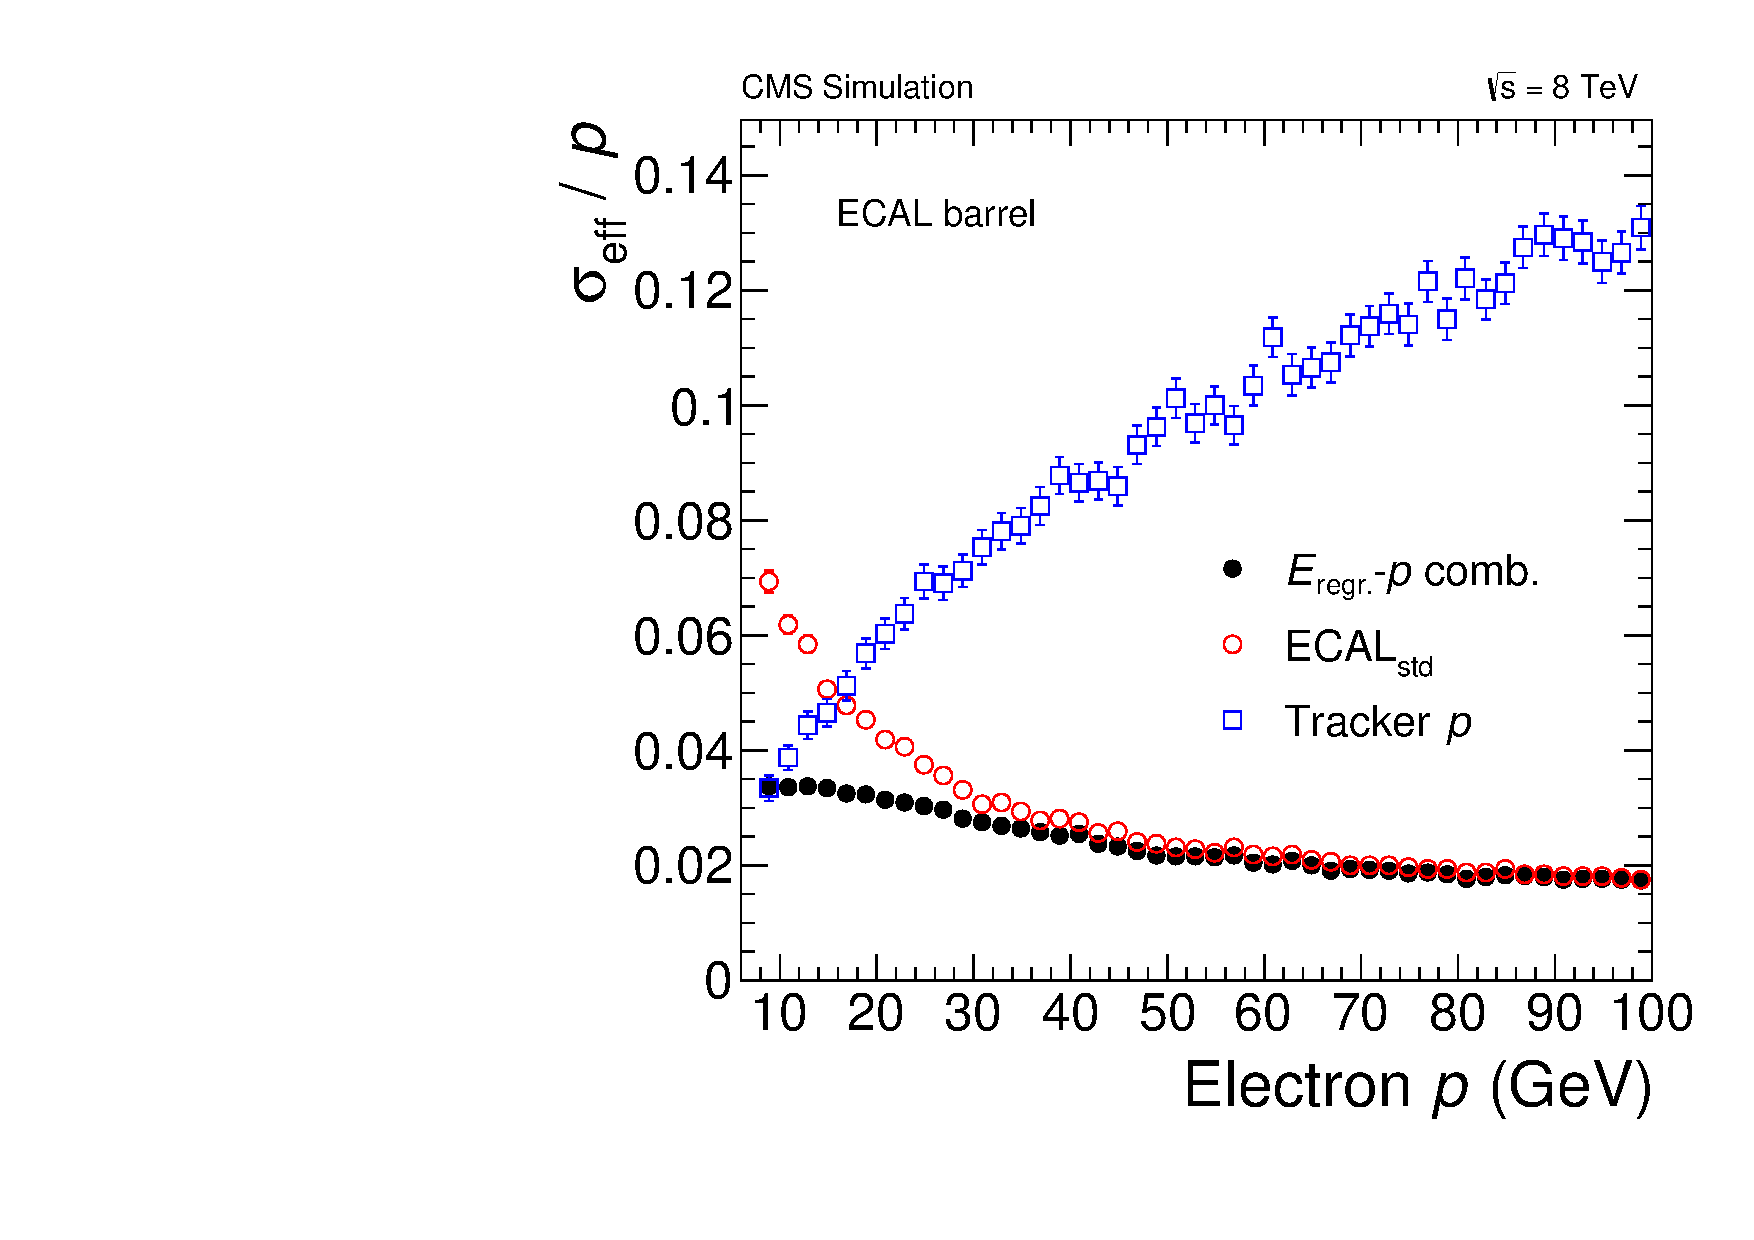
\includegraphics[width=.45\linewidth]{{LHC_CMS/effRMSbarrel_withregression_new}.pdf}
\caption[Effective momentum resolution $\sigma_{\text{eff}}/p$ for electrons in the EB as a function of the momentum for the ECAL-only, the tracker-only, and the combined estimates.]{Effective momentum resolution $\sigma_{\text{eff}}/p$ for electrons in the EB as a function of the momentum for the ECAL-only, the tracker-only, and the combined estimates. \cite{Chatrchyan:2013mxa}.}
\label{fig:ECALresolution}
\end{center}
\end{figure}

\subsection{Hadronic Calorimeter}
\label{sec:HCAL}

The design of the hadron calorimeter (HCAL) is strongly influenced by the choice of magnet parameters because most of the system is located inside the magnet coil and surrounds the ECAL system\cite{Bayatian:922757}. The HCAL system consists of a set of sampling calorimeters. The barrel (HB) and endcap (HE) calorimeters utilize alternating layers of brass as absorber and plastic scintillator as active material. The scintillation light is converted by wavelength-shifting fibers embedded in the scintillator and channeled to hybrid photodiode detectors via clear fibers. The outer calorimeter (HO) uses the CMS magnet and return yoke as the absorber while using the same active material and readout system as HB and HE. The HO system serves as a ``tail-catcher" after the magnet oil, thus reducing the tails in the energy resolution function.

The HCAL is segmented into individual calorimeter cells along three coordinates, $\eta$, $\phi$, and depth. The depth is an integer coordinate that enumerates the segmentation longitudinally, along the direction from the venter of the nominal interaction region. The layout of the system can be seen in figure \ref{fig:HCAL}. The HB system covers the region $-1.4 < \eta < 1.4$ constructed in 2 half barrels. The HE covers the region $1.3 < \abs{\eta} < 3.0$, the segmentation is not uniform in order to maintain coverage and resolution. 

\begin{figure}
\begin{center}
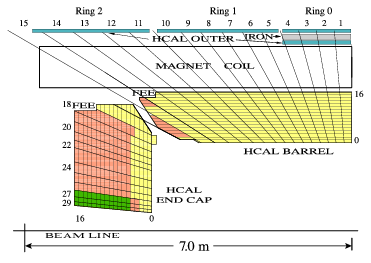
\includegraphics[width=.75\linewidth]{{LHC_CMS/HCALdiagram}.png}
\caption[A quarter slice of the CMS HCAL detectors. The right end of the beam line is the interaction point, HF (not pictured) would be located far to the left. In the diagram, the numbers on the top and left refer to segments in $\eta$, and the numbers on the right and the bottom refer to depth. Colors/shades indicate the combinations of layers that form the different depth segments, which are numbered sequentially starting at 1, moving outward from the interaction point. The outer calorimeter is assigned depth 4. Segmentation along $\phi$ is not shown.]{A quarter slice of the CMS HCAL detectors. The right end of the beam line is the interaction point, HF (not pictured) would be located far to the left. In the diagram, the numbers on the top and left refer to segments in $\eta$, and the numbers on the right and the bottom refer to depth. Colors/shades indicate the combinations of layers that form the different depth segments, which are numbered sequentially starting at 1, moving outward from the interaction point. The outer calorimeter is assigned depth 4. Segmentation along $\phi$ is not shown \cite{Chatrchyan:2009hw}.}
\label{fig:HCAL}
\end{center}
\end{figure}

Coverage between $3.0 < \abs{\eta} < 5.0$ is provided by the steel/quartz fiber hadron forward (HF) calorimeter. HF is unique in that it preferentially samples the neutral component of the hadron shower. This design leads to narrower showers and hence is ideally suited for the congested environment of the forward region. The HF detector is located outside of the muon system, $\unit{11.2}{\meter}$ from the interaction point. Unlike the scintillator that is used in the other HCAL systems, HF uses Cerenkov light emitted in the quartz fibers lay parallel to the beam and are placed in a square grid inside steel plates.

What is actually measured by the HCAL system are particle jets. This is a result of the QCD that was discussed in previous sections and is outlined a bit more in section \ref{sec:TriggerANDreconstruction}. The granularity and sampling of the different components of the HCAL system have been chosen so that the jet energy resolution is similar in all three regions (HB, HE, HF). This is illustrated in figure \ref{fig:HCALresolution} where the jet energy resolution is plotted as a function of the transverse energy. More details on this plot can be found in \cite{Bayatian:922757}.

\begin{figure}
\begin{center}
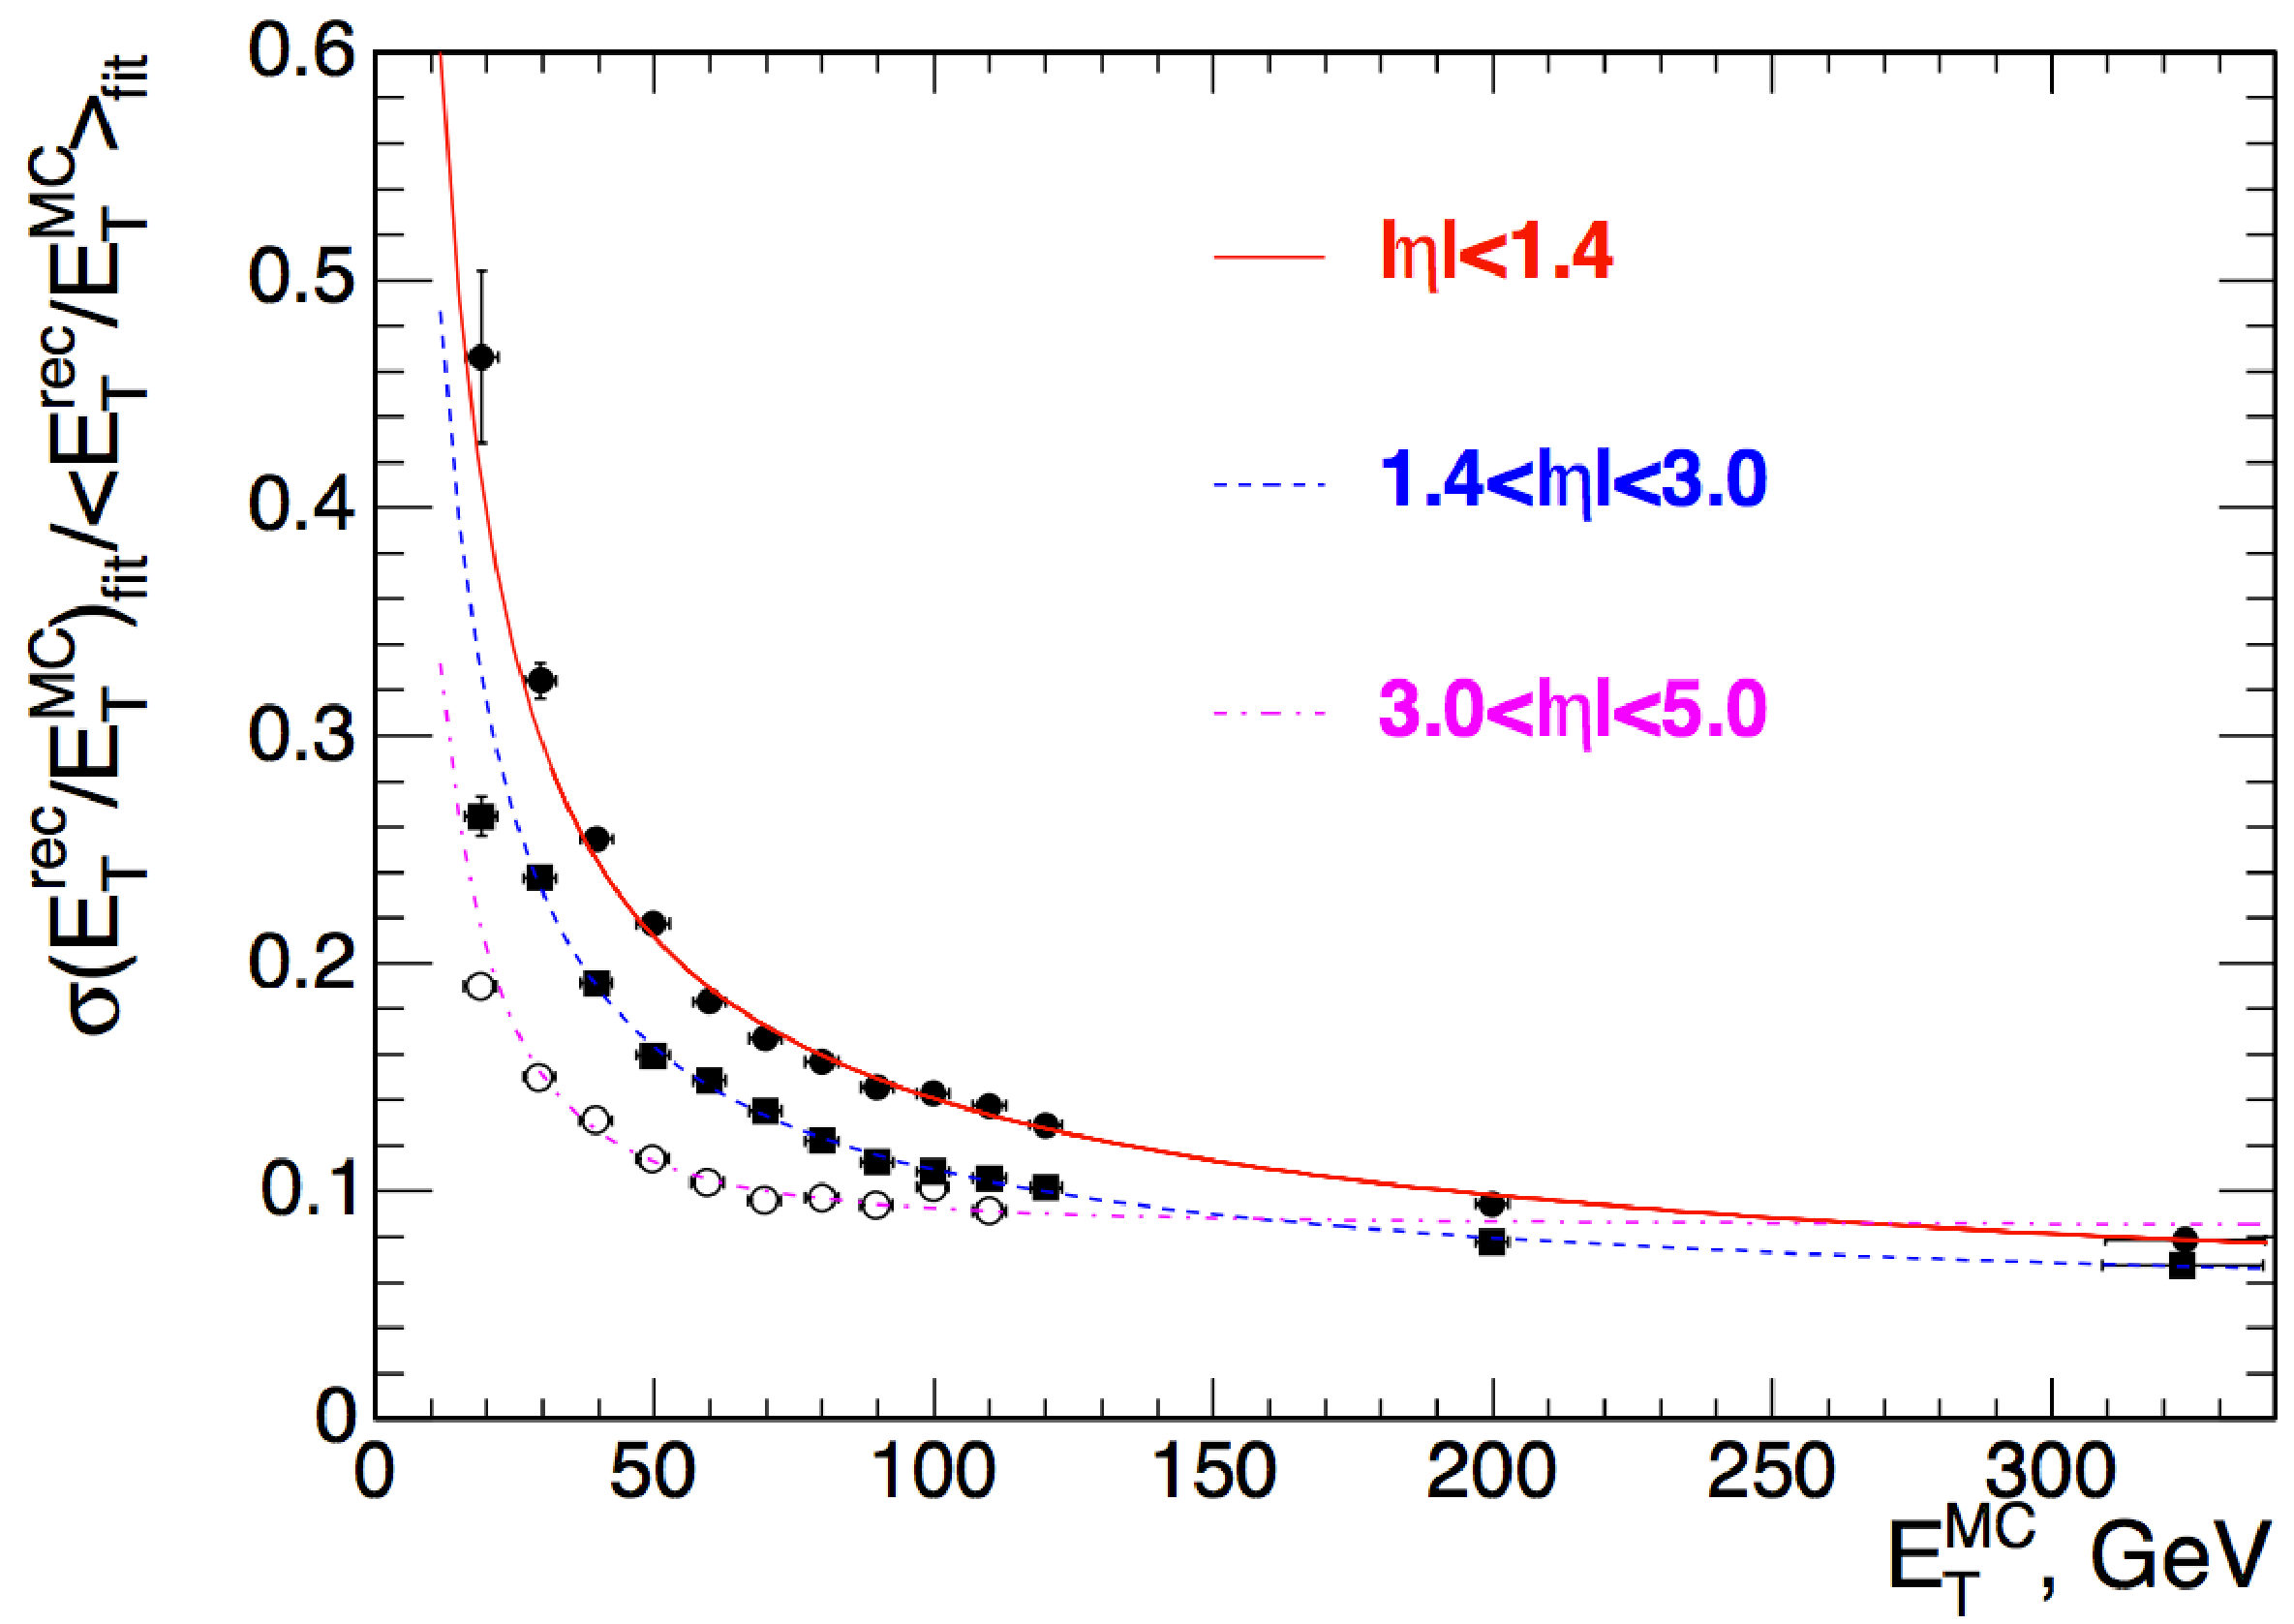
\includegraphics[width=.75\linewidth]{{LHC_CMS/HCALresolution}.pdf}
\caption[The jet transverse energy resolution as a function of the simulated jet transverse energy for barrel jets $\left(\abs{\eta} < 1.4\right)$, endcap jets $\left(1.4< \abs{\eta} <3.0\right)$ and very forward jets $\left(3.0< \abs{\eta} < 5.0\right)$]{The jet transverse energy resolution as a function of the simulated jet transverse energy for barrel jets $\left(\abs{\eta} < 1.4\right)$, endcap jets $\left(1.4< \abs{\eta} <3.0\right)$ and very forward jets $\left(3.0< \abs{\eta} < 5.0\right)$ \cite{Bayatian:922757}.}
\label{fig:HCALresolution}
\end{center}
\end{figure}

\subsection{Muon System}
\label{sec:Muon}

Muons at CMS are measured three times: in the inner tracker, after the magnet coil, and in the return flux. The muon system is designed to measure the path of the muons once they exit the magnet coil and as they traverse the return yoke. The momentum of the muons is measured by the bending angle of the muon's path as they exit the $\unit{4}{\tesla}$ coil taking the interaction point as the origin of the muon. The resolution at the origin of this measurement (hereafter referred to as ``muon system only") is dominated by multiple scatter in the material before the first muon station. This applies up to $p_{T} \sim \unit{200}{\GeVoverc}$, at which point the spatial resolution of the chamber states to dominate. For low-momentum muons, the best momentum resolution is determined by the silicon tracker (``inner tracker only"). However both systems contain information about the momentum and origin of muons, so CMS uses both of them (``full system") in concert to determine the momentum of muons produced in collisions. The momentum resolution can be seen in figure \ref{fig:MuonResolution}.

\begin{figure}
\begin{center}
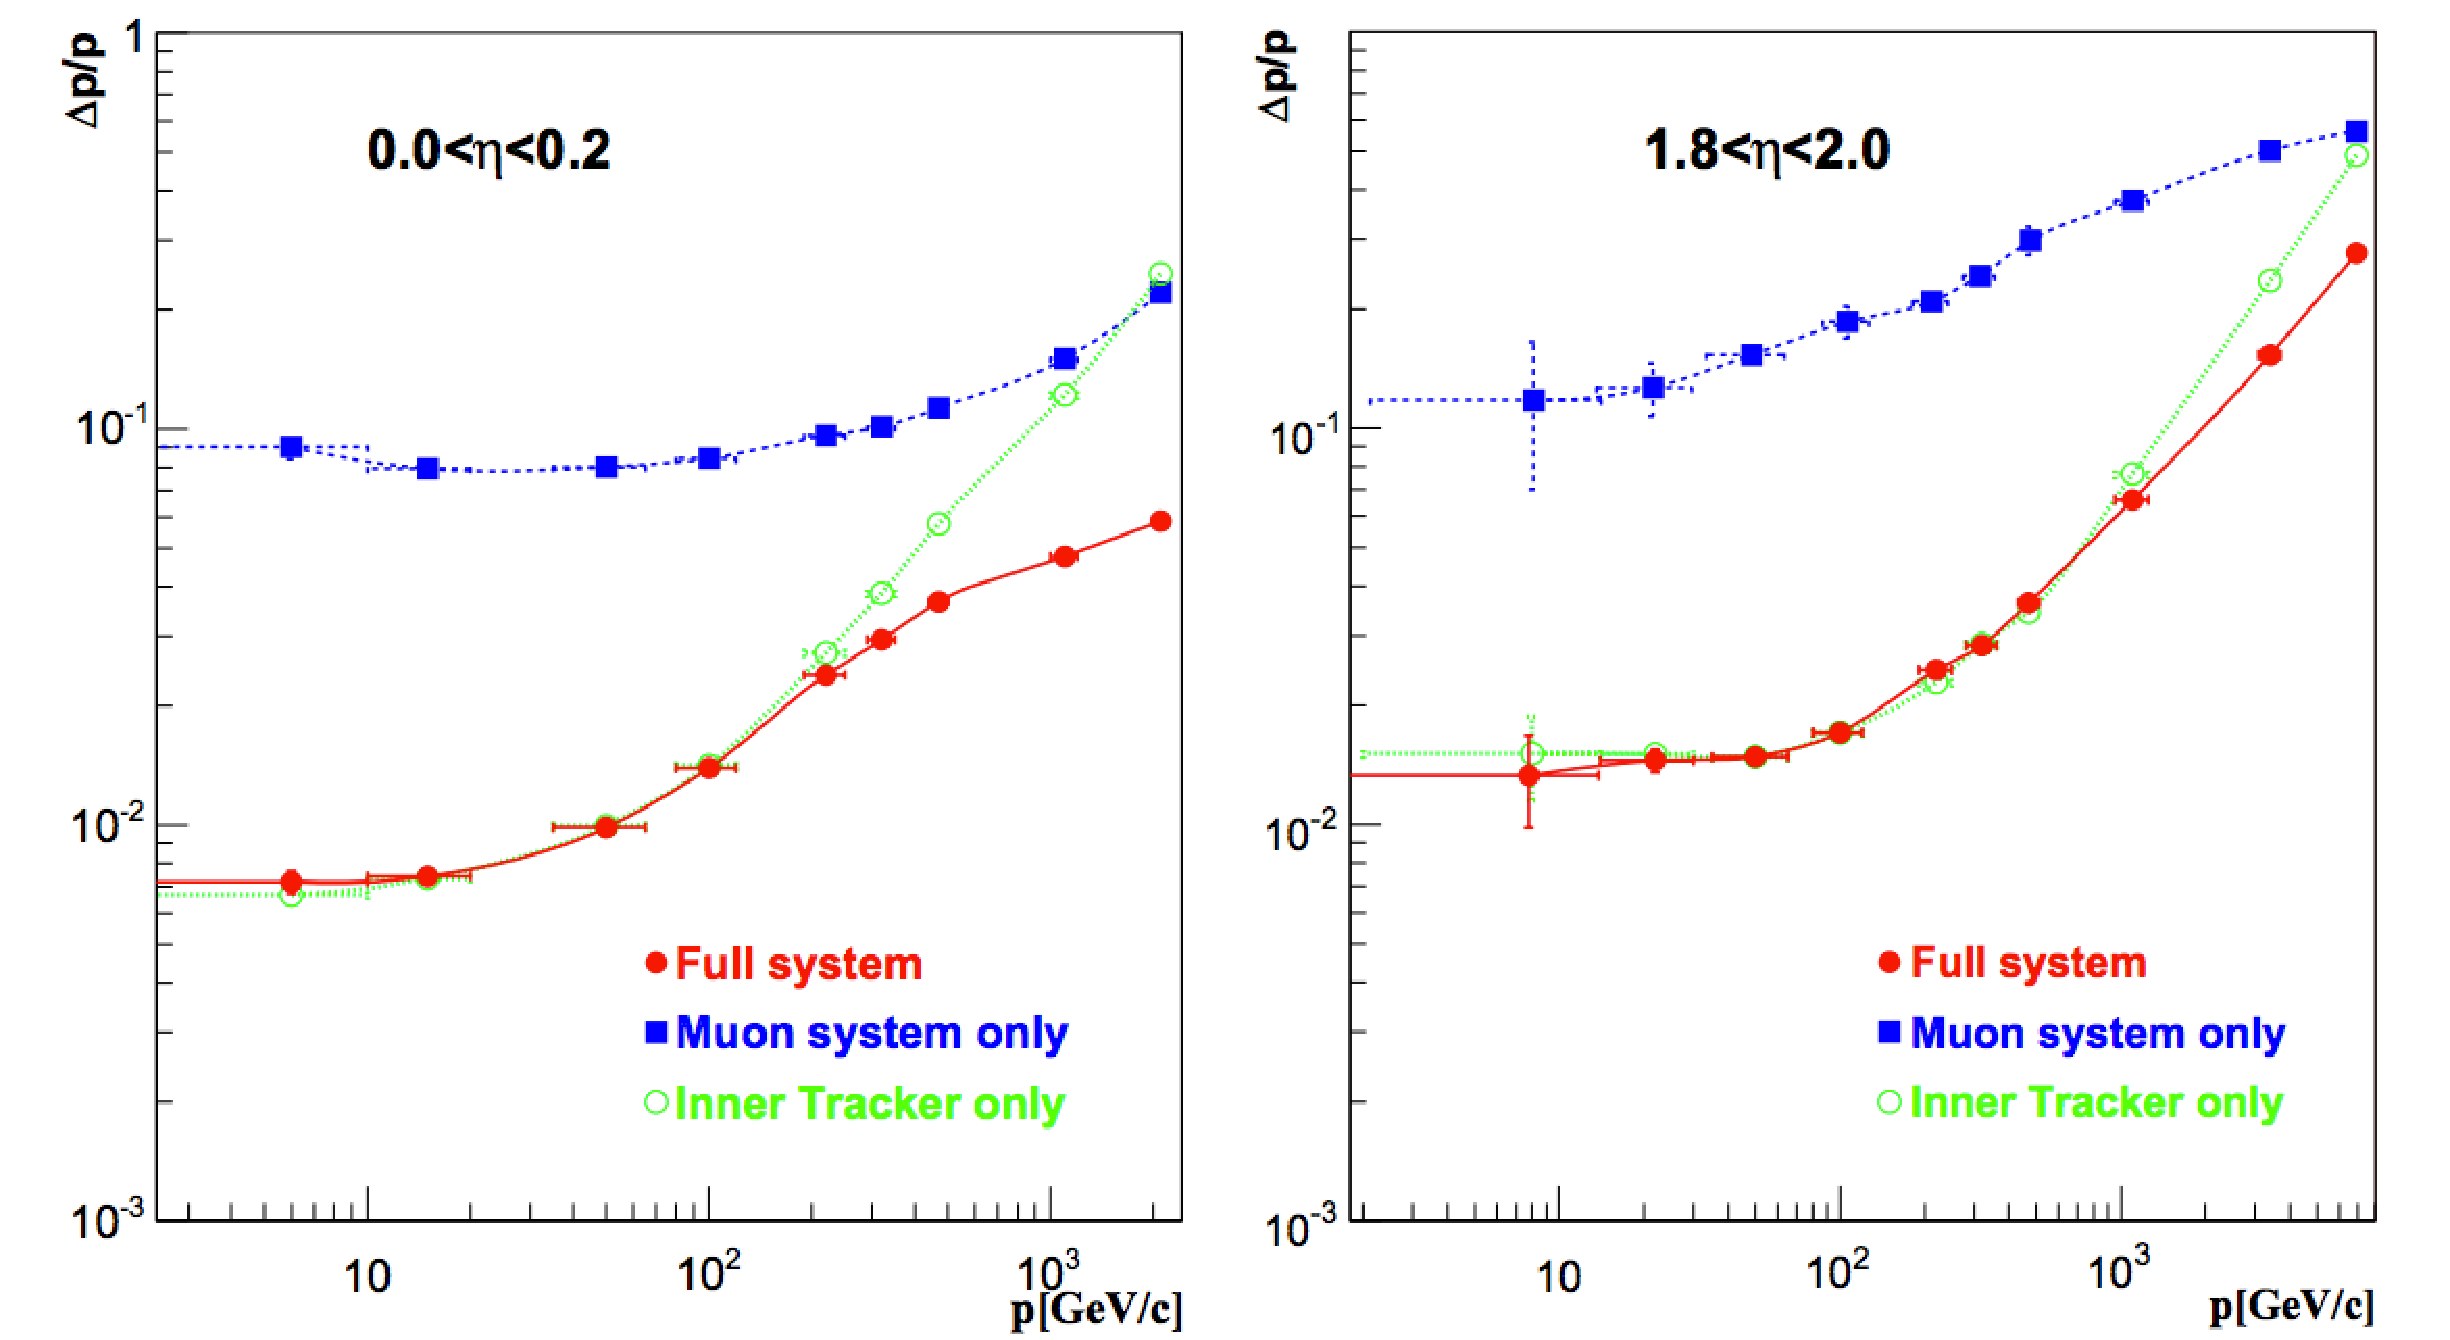
\includegraphics[width=0.75\linewidth]{{LHC_CMS/Muon_Resolution}.pdf}
\caption[The muon momentum resolution verses $p$ using the muon system only, the inner tracker only, or both (``full system"). (left) Barrel $\abs{\eta} < 0.2$ and (right) endcap $1.8 < \abs{\eta} < 2.0$.]{The muon momentum resolution verses $p$ using the muon system only, the inner tracker only, or both (``full system"). (left) Barrel $\abs{\eta} < 0.2$ and (right) endcap $1.8 < \abs{\eta} < 2.0$ \cite{Bayatian:922757}.}
\label{fig:MuonResolution}
\end{center}
\end{figure}

The muon system contains three types of gaseous detectors designed to cover the very large surface and the different radiation environments. The barrel region $\left( \abs{\eta} < 1.2 \right)$ is characterized by low neutron induced background, low muon rate, and low residual magnetic field in the chambers. For these reasons, drift tube (DT) chambers are used. In contrast the endcap region has high muon rates, neutron induced backgrounds, and residual magnetic field. So in the endcaps cathode strip chambers (CSC) are used to cover the region up to $\abs{\eta} < 2.4$. Both the endcap and barrel regions also use resistive plate chambers (RPC) which provide a fast response with good time resolution but lower position resolution than the DT and CSC systems. Taking the time information from the RPCs in concert with the position information from the CSCs and DTs provide necessary and complementary measurements. The whole system provides a precise and flexible detector that can be used for triggering and measurements.

The layout of one quarter of the CMS muon system is shown in figure \ref{fig:MuonDetectors}. In the barrel region, four stations of detectors are arranged in cylinders interlayered with the iron return yoke. The segmentation follows the five wheels of the yoke. In each of the endcaps, the CSC and RPC detectors are arranged with four disks perpendicular to the beam in concentric rings. In total, the muon system contains $\sim\unit{25000}{\squaremetre}$ of active detection planes with $\sim 1$ million electronic channels.

\begin{figure}
\begin{center}
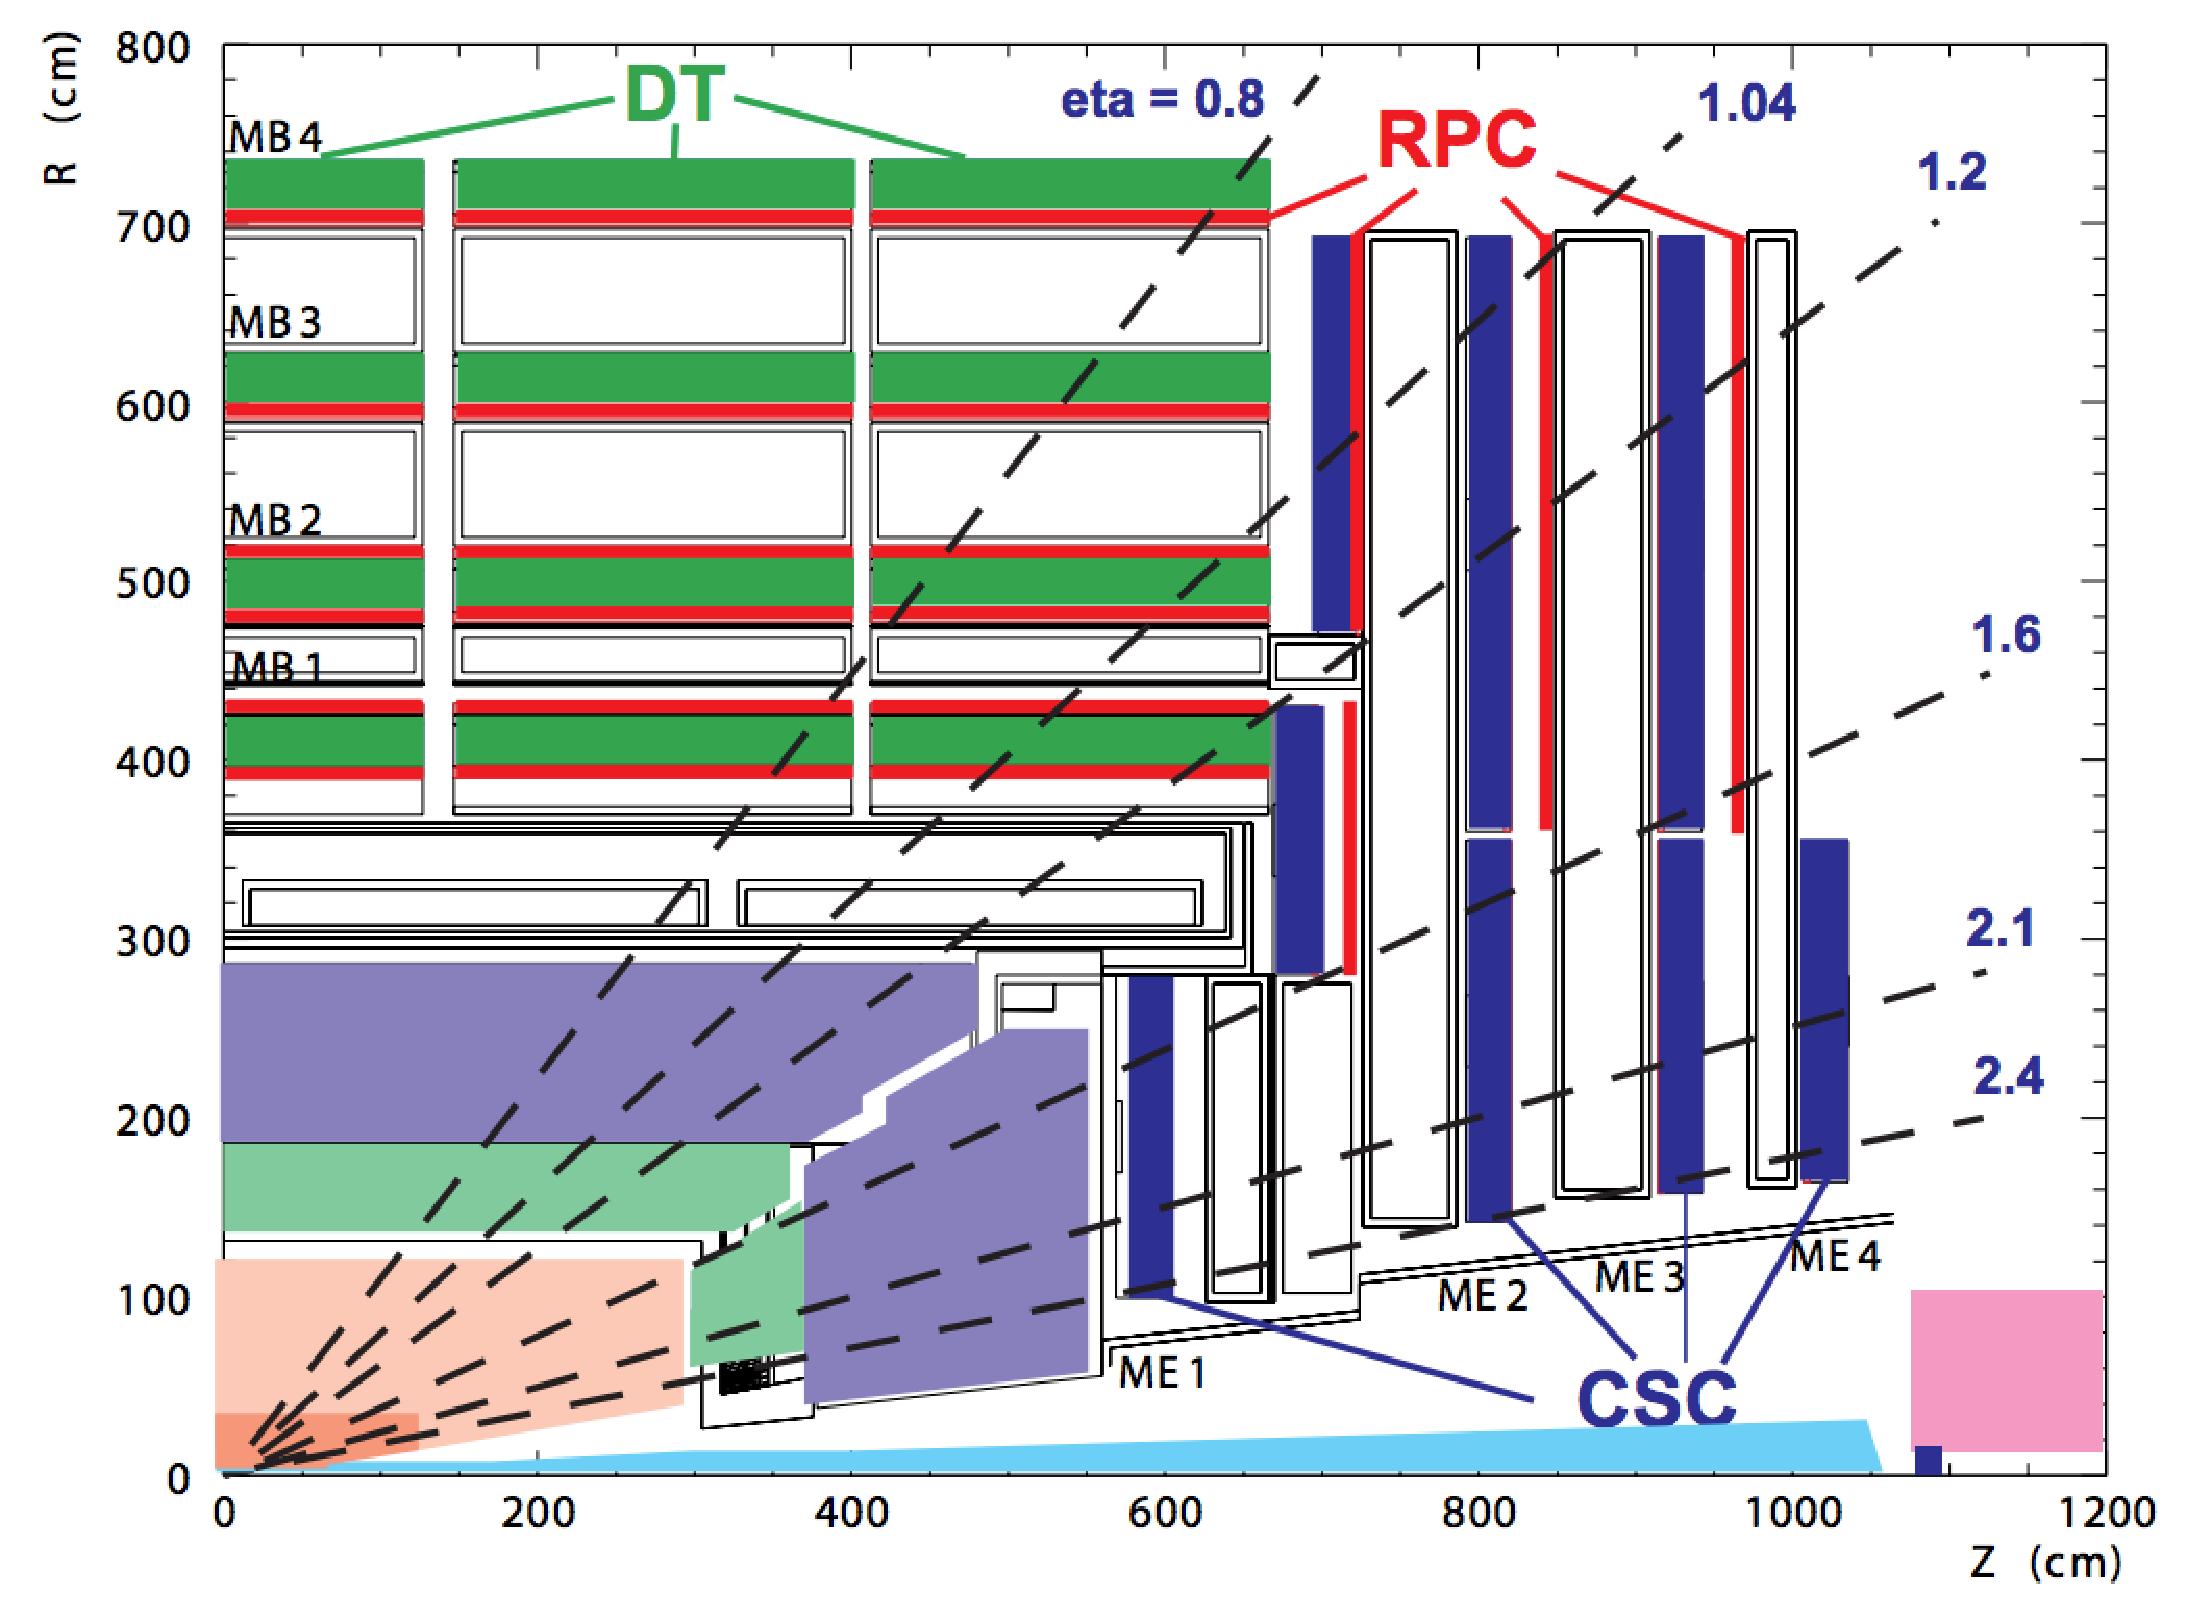
\includegraphics[width=0.75\linewidth]{{LHC_CMS/Muon_Detectors}.pdf}
\caption[Layout of one quarter of the CMS muon system for initial low luminosity running. The RPC system is limited to $\abs{\eta} < 1.6$ in the endcap, and for the CSC system only the inner ring of the ME4 chambers have been deployed]{Layout of one quarter of the CMS muon system for initial low luminosity running. The RPC system is limited to $\abs{\eta} < 1.6$ in the endcap, and for the CSC system only the inner ring of the ME4 chambers have been deployed\cite{Bayatian:922757}.}
\label{fig:MuonDetectors}
\end{center}
\end{figure}

The barrel detectors consist of 250 chambers organized in four layers inside the magnet return yoke, at radii of approximately $\unit{4.0, 4.9, 5.9, 7.0}{\meter}$ from the beam axis. Each DT chamber in the three innermost stations consists of 12 layers of drift tubes divided into three groups of four consecutive layers, hereafter called SuperLayers (SL). The tubes inside each SL are staggered by half a tube. Two SLs measure the $r-\phi$ coordinate in the bending plane (they have wires parallel to the beam line), and the third SL measures the $z$-coordinate running parallel to the beam.  In the outermost station each DT chamber has only the two SLs that measure the $r-\phi$ coordinate. The two innermost stations consist of �sandwiches� made of a DT chamber placed between 2 RPCs. The two outermost stations consist of packages of a DT chamber coupled to a layer made of 1, 2, or 4 RPCs, depending on the sector and station, placed on the innermost side of the station. The maximum drift length in the barrel is $\unit{2.0}{\centi\meter}$ and the single-point resolution is $\sim \unit{200}{\micro\meter}$, giving a $\phi$ precision better than $\unit{100}{\micro\meter}$ in position and approximately $\unit{1}{\milli\rad}$ in direction.

In the two endcaps, 468 CSCs arranged in four stations of chambers which are mounted in disks enclosing the CMS magnet, perpendicular to the beam direction. Each CSC is a trapezoidal in shape and consists of six gas gaps, each gap having a plane of radial cathode strips and plane of anode wires running almost perpendicularly to the strips. Most CSCs are overlapped in $\phi$ to avoid gaps in the muon acceptance\footnote{The exception being the third ring of the first endcap disk.}. Each ring station consists of 36 chambers, except for the innermost ring of the second, third, and fourth disks which have 18 chambers. A precise position measurement is made by determining the center-of-gravity of the charge distribution induced on the cathode strips with a spatial resolution $\sim\unit{200}{\micro\meter}$ and angular resolution in $\phi \sim \unit{10}{\milli\rad}$. Like in the Barrel, there are layers of double-gap RPCs in the endcaps, however, for the initial low-luminosity run there are RPCs only in the outer rings of each station, while they are staged in the internal rings. The RPC endcap system is thus limited to $\eta < 1.6$ for the first period of data taking.

\section{Triggering and Particle Reconstruction}
\label{sec:TriggerANDreconstruction}

At the designed specifications the LHC would lead to $\sim 10^{9}$ interactions/sec. Data from only about $10^{2}$ crossings/sec can be written to archival media; hence, the trigger system has to achieve a rejection factor $10^{6}$. This is performed by the CMS trigger and data acquisition system which consists of four parts: the detector electronics, the Level-1 trigger, the readout network, and an online event filter system (processor farm) that executes the software for the High-Level Triggers (HLT).

Once the data is archived, CMS must analyze this data and reconstruct the individual particles that make up the event. A particle flow event-reconstruction algorithm (PF) has been successfully deployed in the CMS experiment and is nowadays used by most of the analyses. It aims at identifying and reconstructing individually each particle arising from the LHC proton-proton collision, by combining the information from all the subdetectors. Using this algorithm individual particles can be identified as photons, electrons, muons, or charged/neutral hadrons.

\subsection{CMS Trigger}

The size of the LHC detectors and the underground caverns that they reside in imposes a minimum transit time for the signals from the front-end electronics to reach the services cavern which houses the Level-1 trigger logic. A signal must pass from the various subdetectors we have discussed to this Level-1 system and back again to signal a readout of the full detector. The total time allocated for the transit and for reaching a decision to keep or discard data from a particular beam crossing is $\unit{3.2}{\micro\second}$. During this time, the detector data is held in buffers while trigger data is collected form the front-end electronics and decisions reached that discard a large fraction of events while regaining the small fraction of interactions of interest (approx. 1 in 1000). Of the total latency, the time allocated to the Level-1 trigger calculations is less than $\unit{1}{\micro\second}$.

Custom hardware processors form the Level-1 decision. The Level-1 triggers involve the calorimetry and muons systems, as well as some correlation of the information between these systems. These Level-1 decisions are based on the presence of ``trigger primitive" objects such as photons, electrons, muons, and jets above a set of $E_{T}$ and $p_{T}$ thresholds that have reduced granularity and resolution. It also employs global sums of $E_{T}$ and $E_{T}^{\text{miss}}$. The designed Level-1 pass rate is $\unit{100}{\kilo\hertz}$, but was limited to $\unit{50}{\kilo\hertz}$ at startup.

Upon receipt of a Level-1 trigger, the data from the pipelines are transferred to front-end readout buffers. After further signal processing, zero-suppression and/or data-compression each event will have a size of about $\unit{1.5}{\mega\text{B}}$ for proton-proton interactions. Data from a given event are then transferred to a processor that runs the high-level trigger (HLT) software to reduce the Level-1 output rate of $\unit{100}{\kilo\hertz}$ down to $\unit{100}{\hertz}$ for mass storage. Rather than reconstruct all possible objects in an event for HLT, whenever possible only those objects and regions of the detector that are actually needed for the decision are reconstructed. In that way events are discarded as soon as possible, events that still pass are then stored across the ``LHC Computing Grid"\footnote{Specifics of this vast and complex GRID computing network are not discussed here.} for later software analysis by individuals searching for specific physics phenomenon.

\subsection{Particle Flow}

The particle-flow event reconstruction aims at reconstructing and identifying all stable particles in the event, i.e., electrons, muons, photons, charged hadrons and neutral hadrons, with a thorough combination of all CMS sub-detectors towards an optimal determination of their direction, energy and type. This list of individual particles is then used to build jets (from which the quark and gluon energies and directions are inferred), to determine the missing transverse energy $E_{T}^{\text{miss}}$ (which gives an estimate of the direction and energy of the neutrinos and other invisible particles), to reconstruct and identify taus, $\tau$, from their decay products, to quantify charged lepton isolation with respect to other particles, to tag $b$ jets, etc \cite{CMS-PAS-PFT-09-001}.

While this algorithm is extremely versatile we will focus our discussion on the pieces that are relevant for this analysis: electrons, muons, and jets. A small discussion will also be made of photons which are used in this analysis as well. 

\subsection{Electrons}

The electron reconstruction combines ECAL and tracker information. Electron candidates are reconstructed from clusters of energy deposits in the ECAL, which are then matched to hits in the silicon tracker and silicon tracker seeds that are mapped to ECAL clusters. This dual approach improves the reconstruction efficiency for the very low $p_{T}$ electrons. The CMS electron reconstruction algorithm is described in \cite{CMS-PAS-EGM-10-004,Chatrchyan:2013mxa}. 

For this physics analysis, the electron candidates are required to have transverse momentum $p^{e}_{T} > \unit{7}{\GeVoverc}$ and a reconstructed $\abs{\eta} < 2.5$. The reconstruction efficiency for isolated electron is expected to be above 90\% over the full ECAL acceptance, apart from some narrow ``crack" regions. 

The identification of electrons relies on a Boosted Decision Tree (BDT) multivariate technique that combines observables sensitive to the amount of bremsstrahlung along the electron trajectory, the geometrical and momentum matching between the electron trajectory and associated clusters, as well as shower-shape observables. The distribution of expected and observed electron BDT output is shown in figure \ref{fig:Ele_BDT}. The selection is optimized in six regions of the electron $p^{e}_{T}$ and $\abs{\eta^{e}}$ to maximize
the expected sensitivity for a low-mass Higgs boson. These regions correspond to two $p^{e}_{T}$ ranges, $\unit{7--10}{\GeV}$ and $>\unit{10}{\GeV}$, and three pseudorapidity regions, corresponding to two regions in the barrel with different material in front of the ECAL, the central barrel $\left(\abs{\eta^{e}} < 0.8\right)$ and the outer barrel $\left(0.800 < \abs{\eta^{e}} < 1.479\right)$, in addition to the endcap, $1.479 < \abs{\eta^{e}} < 2.500$.

\begin{figure}
\begin{center}
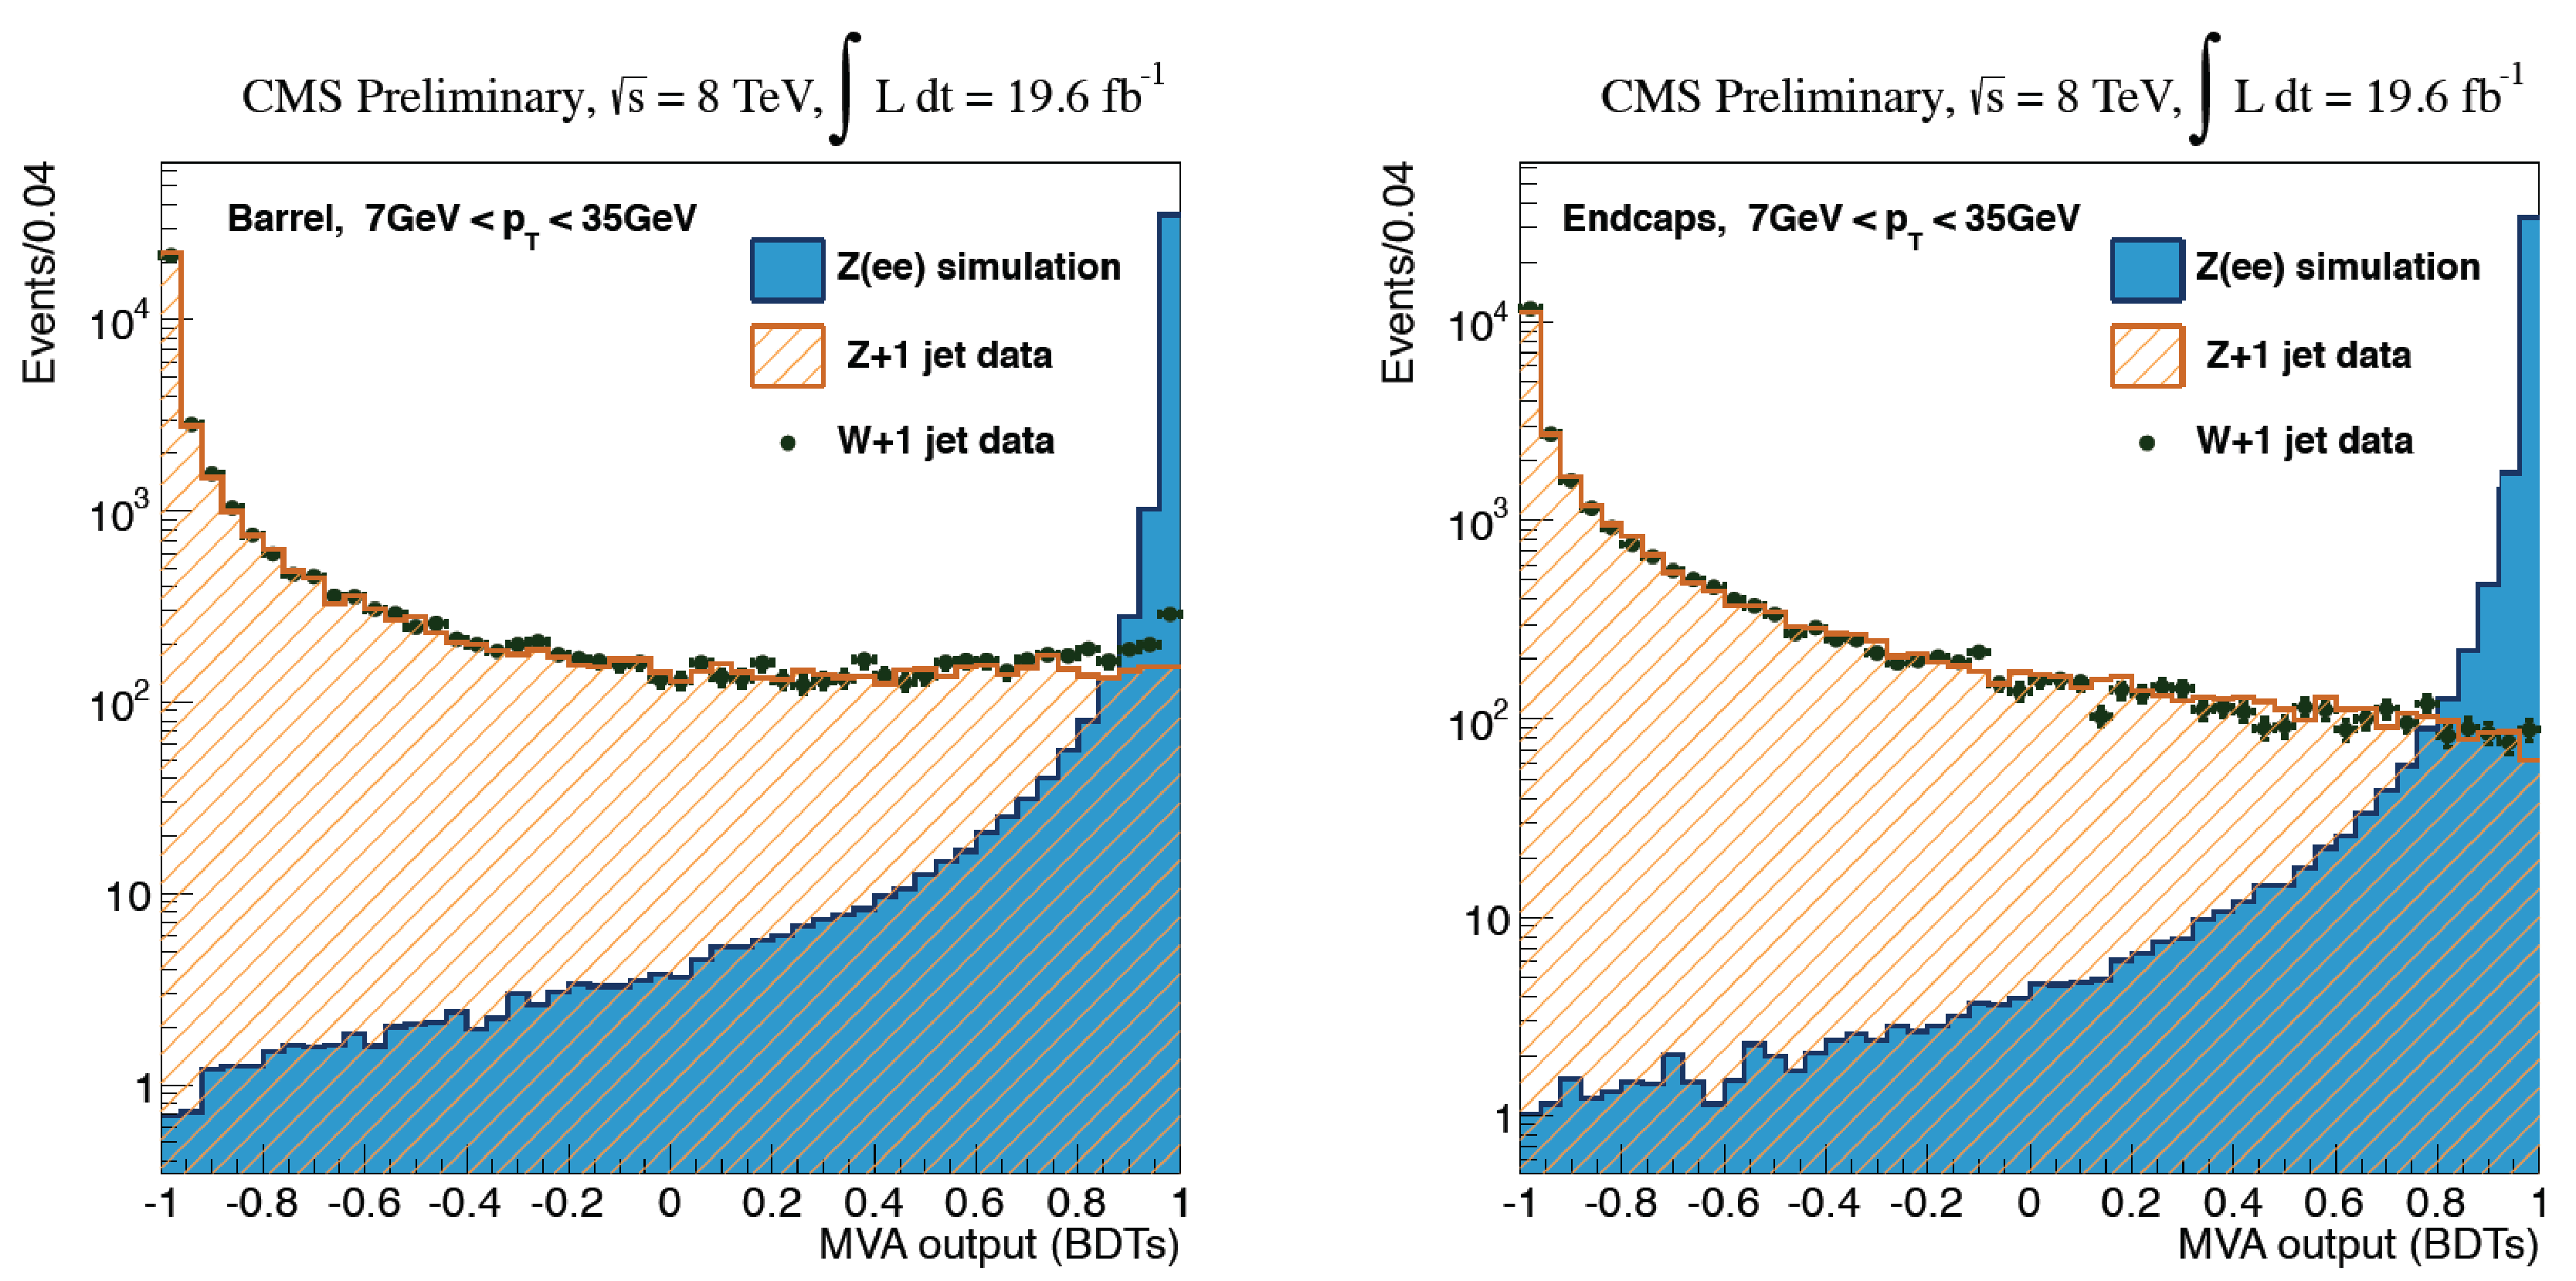
\includegraphics[width=0.75\linewidth]{{LHC_CMS/Ele_BDT}.pdf}
\caption[Distribution of electron BDT output for training sample $W+$jets, test sample $Z+$jets on 2012 data (fakes) and prompt electrons ($Z \to ee$ simulation) in the barrel (left) and endcap(right)]{Distribution of electron BDT output for training sample $W+$jets, test sample $Z+$jets on 2012 data (fakes) and prompt electrons ($Z \to ee$ simulation) in the barrel (left) and endcap(right)\cite{CMS-DP-2013-003}.}
\label{fig:Ele_BDT}
\end{center}
\end{figure}

The quality of the momentum measurement for electrons can substantially vary depending on the electron characteristics. The resolution is mainly dominated by the fluctuations of the measured energy due to bremsstrahlung in the tracker material. This entails that the $4\ell$ mass resolution varies broadly, by as much as a factor of 2-3. Therefore, mixing together events with well and poorly measured $4\ell$ masses dilutes the Higgs boson search sensitivity, and mass measurement. The analysis uses the propagation of the lepton uncertainty to estimate the $4\ell$ mass to proper accounting for the signal mass resolutions for individual events. In order to have a good determination of this uncertainty, but above all to have a description of the resolution of the signal model which corresponds to the data, we need to measure it on high statistics control samples, depending on the electron kinematics and quality, which is done with $Z \to ee$ sample. The absolute scale has also to be calibrated on data, because the measurement of the Higgs boson mass depends crucially on the uncertainty that we can assign to the leptons in the full phase space of the analysis for a $\unit{125}{\GeV}$ Higgs boson, so covering from $\unit{7--100}{\GeV}$, which can be covered with $Z \to ee$ and low mass resonances.

For electrons, the calibration procedure consists of three steps. First, a set of corrections for the momentum scale is obtained by comparing the displacement of the peak position in the distributions of the Z-boson mass in the data and in the simulation in different $\eta$ regions and in two categories depending on the amount of bremsstrahlung. The corrections are derived as a function of time in order to account for the time-dependent crystal transparency loss. Second, a linearity correction to the momentum scale is applied to account for the $p_{T}$-dependent differences between data and simulation by comparing the dielectron mass distributions, binned in $p^{e}_{T}$ of one of the two electrons, in data and in simulated $Z \to ee$ events. The $J/\psi \to ee$ and $\Upsilon\left(1S\right) \to ee$ events are used as validation for electron $p^{e}_{T} < \unit{20}{\GeV}$. All the corrections on the electron momentum scale from the first two steps are applied to data. The left of figure \ref{fig:Ele_scale_res} shows the residual momentum scale difference before the linearity correction but after the time dependent corrections. Third, the energies of single electrons in the simulation are smeared by applying a random Gaussian multiplicative factor of mean 1 and width $\Delta\sigma$, in order to achieve the resolution observed in the data Z-boson sample. The result of this resolution correction is shown on the right of figure \ref{fig:Ele_scale_res}.

After the electron calibration, the relative momentum scale between data and simulation is consistent within 0.6\% in the central barrel and up to $\sim 1.5\%$ in the forward part of the ECAL endcaps. The residual dependence at low momentum is due to the use of wide bins in measured electron $p^{e}_{T}$ in evaluating the Z-peak mass shift. The resulting shift of 0.3\% (0.1\%) for the $4e \left(2e2\mu\right)$ channel is assigned as a systematic uncertainty in the signal mass scale.

\begin{figure}
\begin{center}
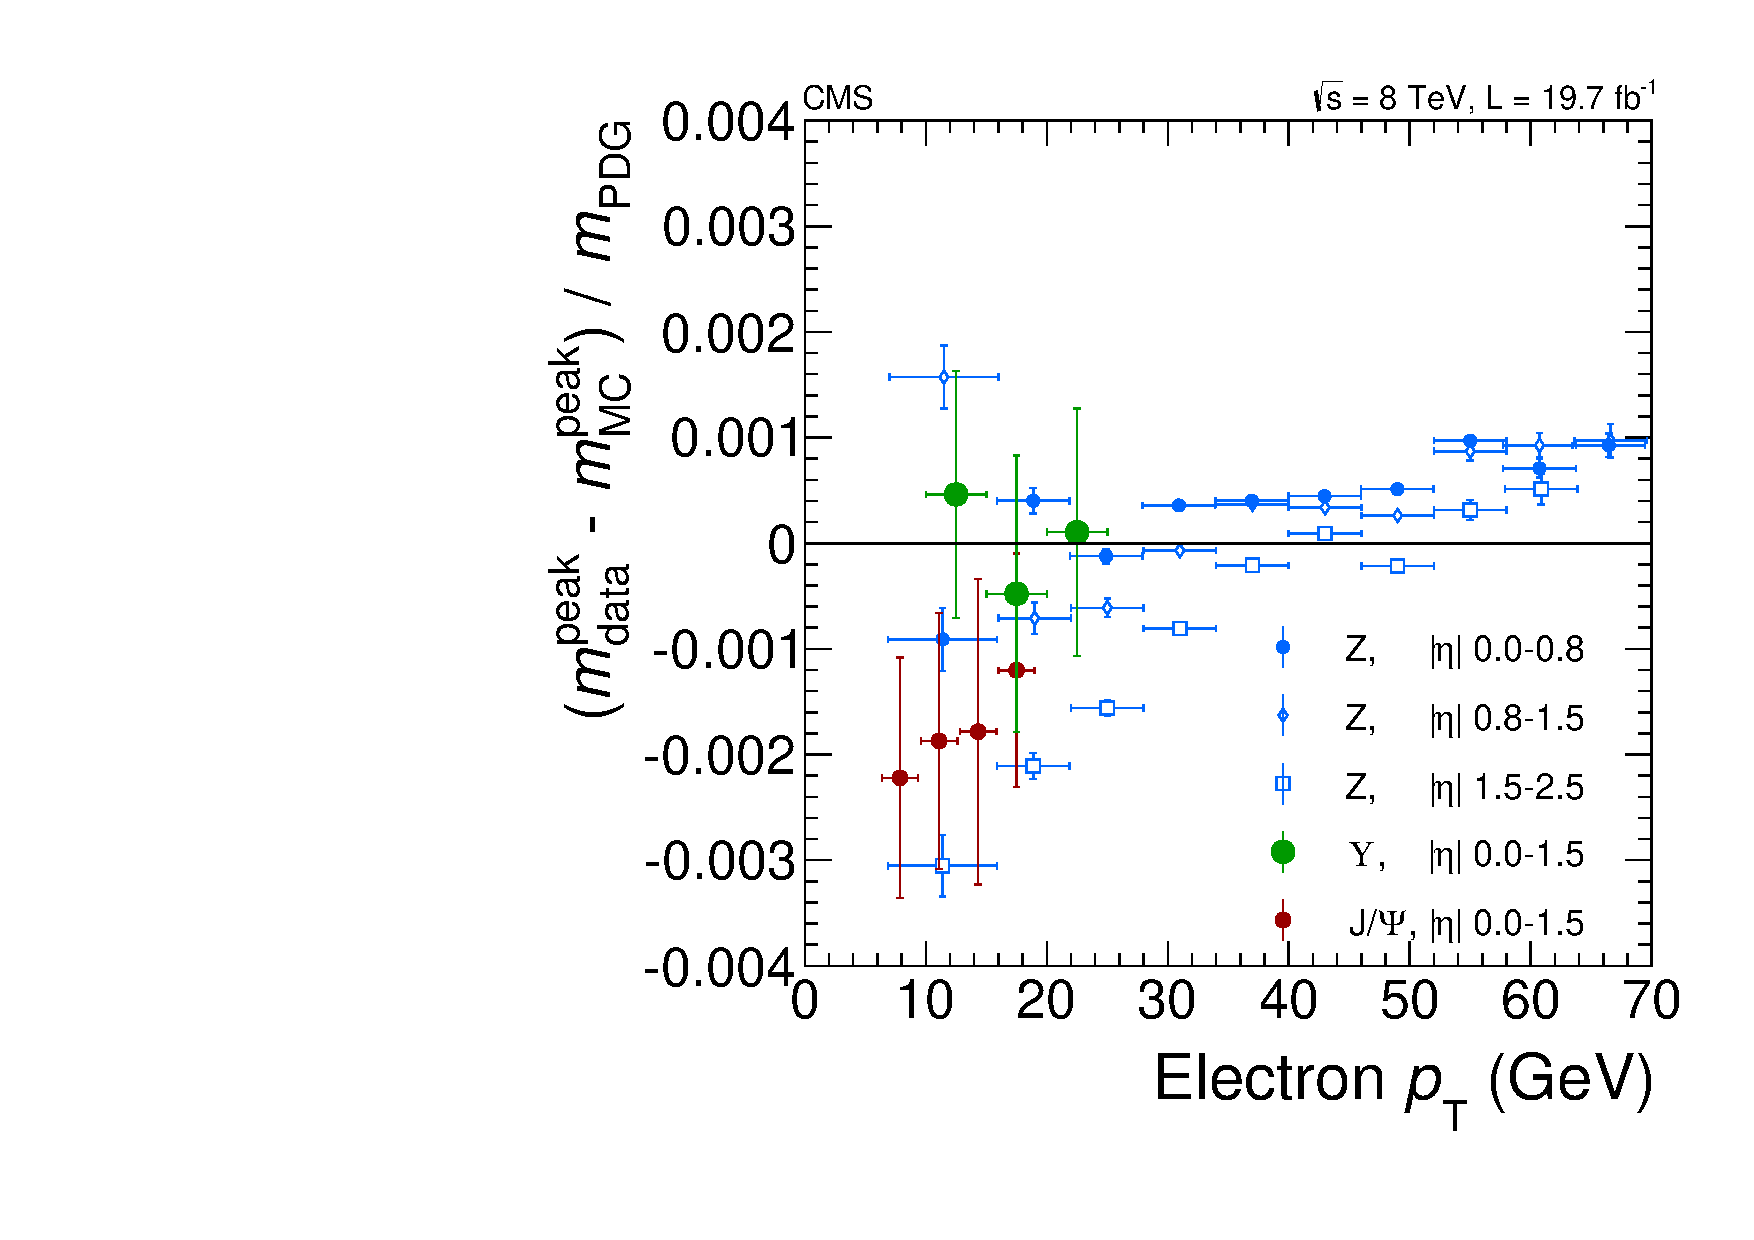
\includegraphics[width=0.45\linewidth]{{LHC_CMS/scale-ptdep-8TeV}.pdf}
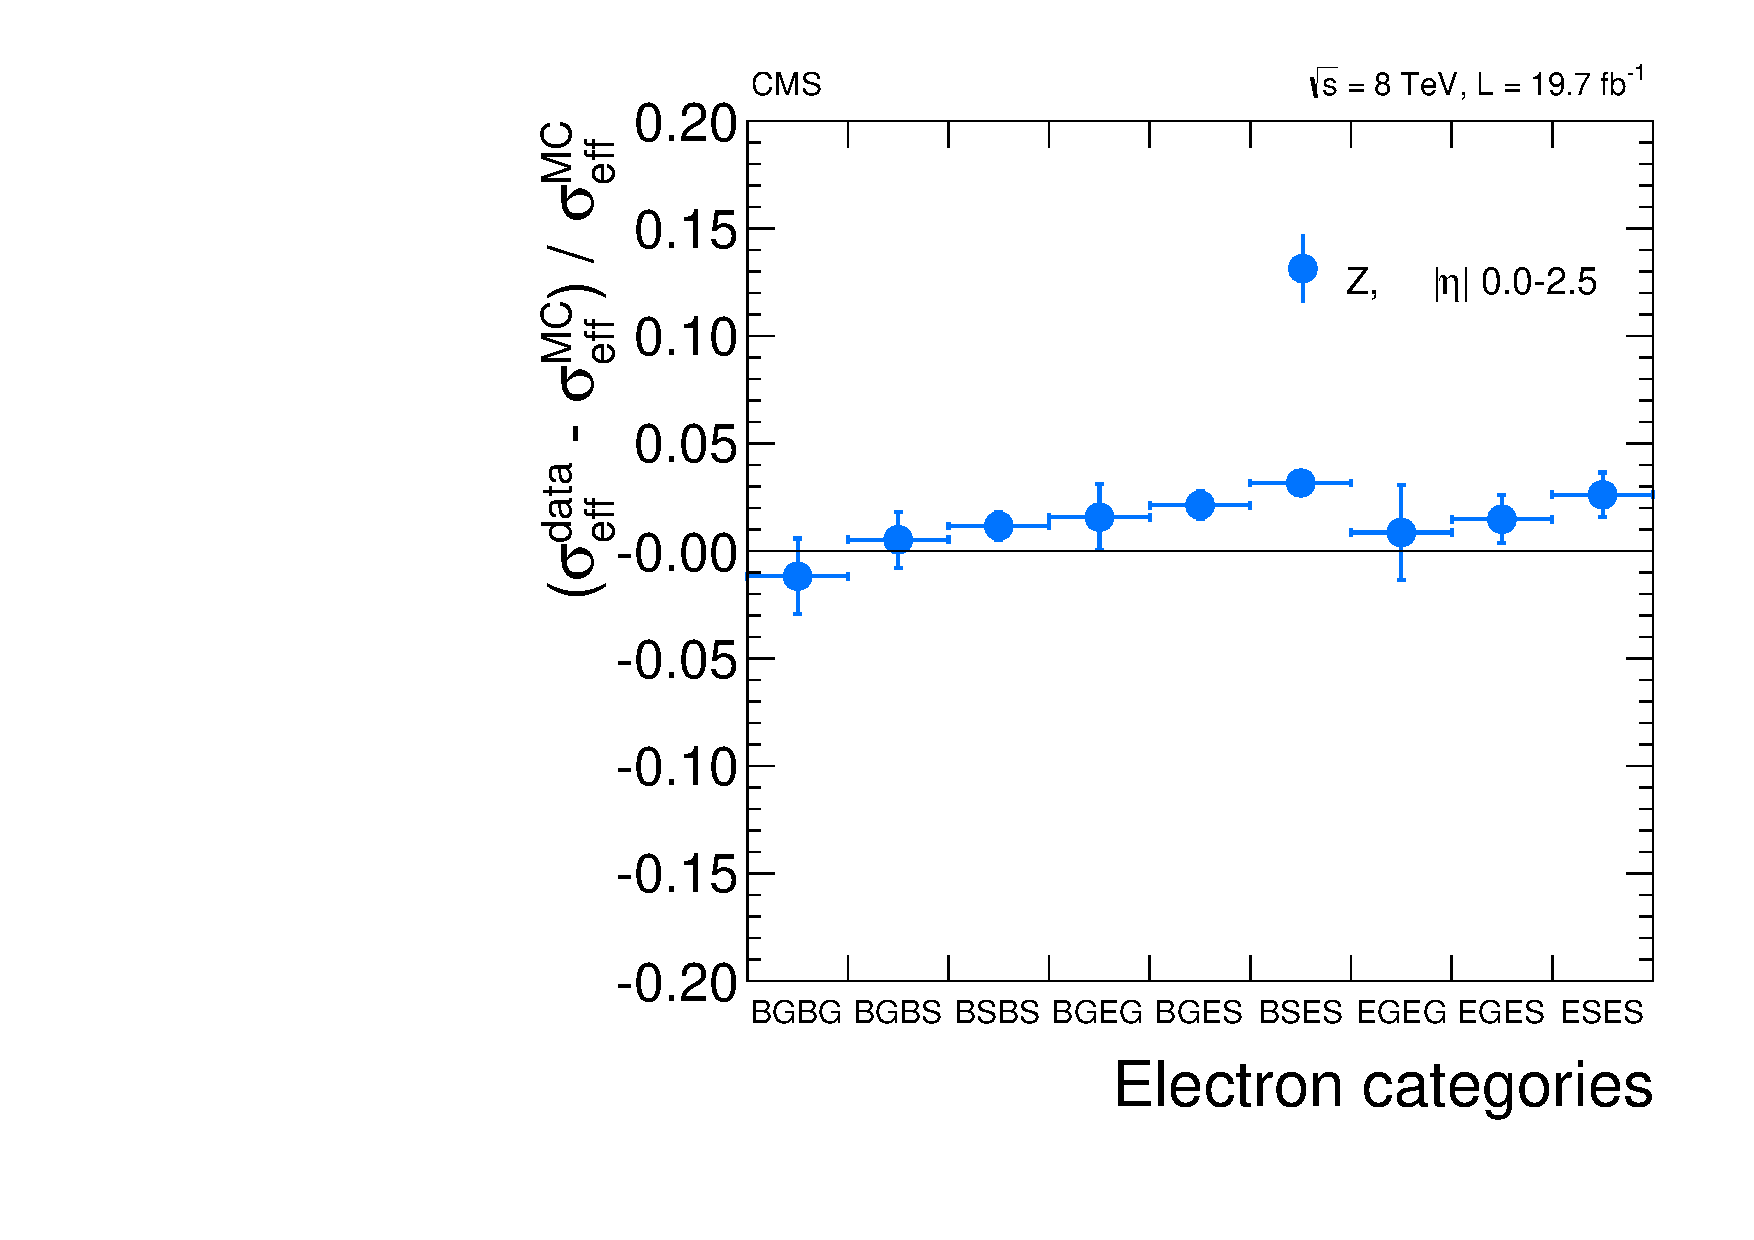
\includegraphics[width=0.45\linewidth]{{LHC_CMS/electron_resolution}.pdf}
\caption[(left) Relative difference between the dilepton mass peak positions in data and simulation as obtained from Z, $J/\psi$ and $\Upsilon\left(nS\right)$ resonances as a function of the transverse momentum of one of the electrons regardless of the second for dielectron events before $p_{T}$ dependent correction. (right) Relative difference between the dilepton mass peak positions in data and simulation as obtained from Z, $J/\psi$ and $\Upsilon\left(nS\right)$ resonances as a function of the transverse momentum of one of the electrons regardless of the second for dielectron events.]{(left) Relative difference between the dilepton mass peak positions in data and simulation as obtained from Z, $J/\psi$ and $\Upsilon\left(nS\right)$ resonances as a function of the transverse momentum of one of the electrons regardless of the second for dielectron events before $p_{T}$ dependent correction. (right) Relative difference between the dilepton mass peak positions in data and simulation as obtained from Z, $J/\psi$ and $\Upsilon\left(nS\right)$ resonances as a function of the transverse momentum of one of the electrons regardless of the second for dielectron events\cite{Chatrchyan:2013mxa}.}
\label{fig:Ele_scale_res}
\end{center}
\end{figure}

\subsection{Muons}
\label{sec:Muons}

Muon candidates are required to have a transverse momentum $p^{\mu}_{T} > \unit{5}{\GeV}$ and be within the geometrical acceptance, defined by $\abs{\eta^{\mu}} < 2.4$. The reconstruction combines information from both the silicon tracker and the muon system. The matching between track segments is done either outside-in, starting from a track in the muon system, or inside-out, starting from a track in the silicon tracker. The muons are selected among the reconstructed muon track candidates by applying minimal requirements on the track segments in both the muon system and inner tracker system and taking into account compatibility with small energy deposits in the calorimeters\cite{Chatrchyan:2013mxa}.

For muons, an absolute measurement of momentum scale and resolution is performed by using a reference model of the Z line shape convolved with a Gaussian function. The bias in the reconstructed muon $p_{T}$ is determined from the position of the Z mass peak as a function of muon kinematic variables, and a correction is derived for the data. A correction for the resolution is also derived for the simulation from a fit to the $Z \to \mu\mu$ mass spectrum. The large event sample based on low-mass dimuon resonances provides an additional calibration source for the momentum resolution in a similar manner. For muons, the agreement between the observed and simulated mass scales is within 0.1\% in the entire pseudorapidity range of interest and assigned as a systematic.

\begin{figure}
\begin{center}
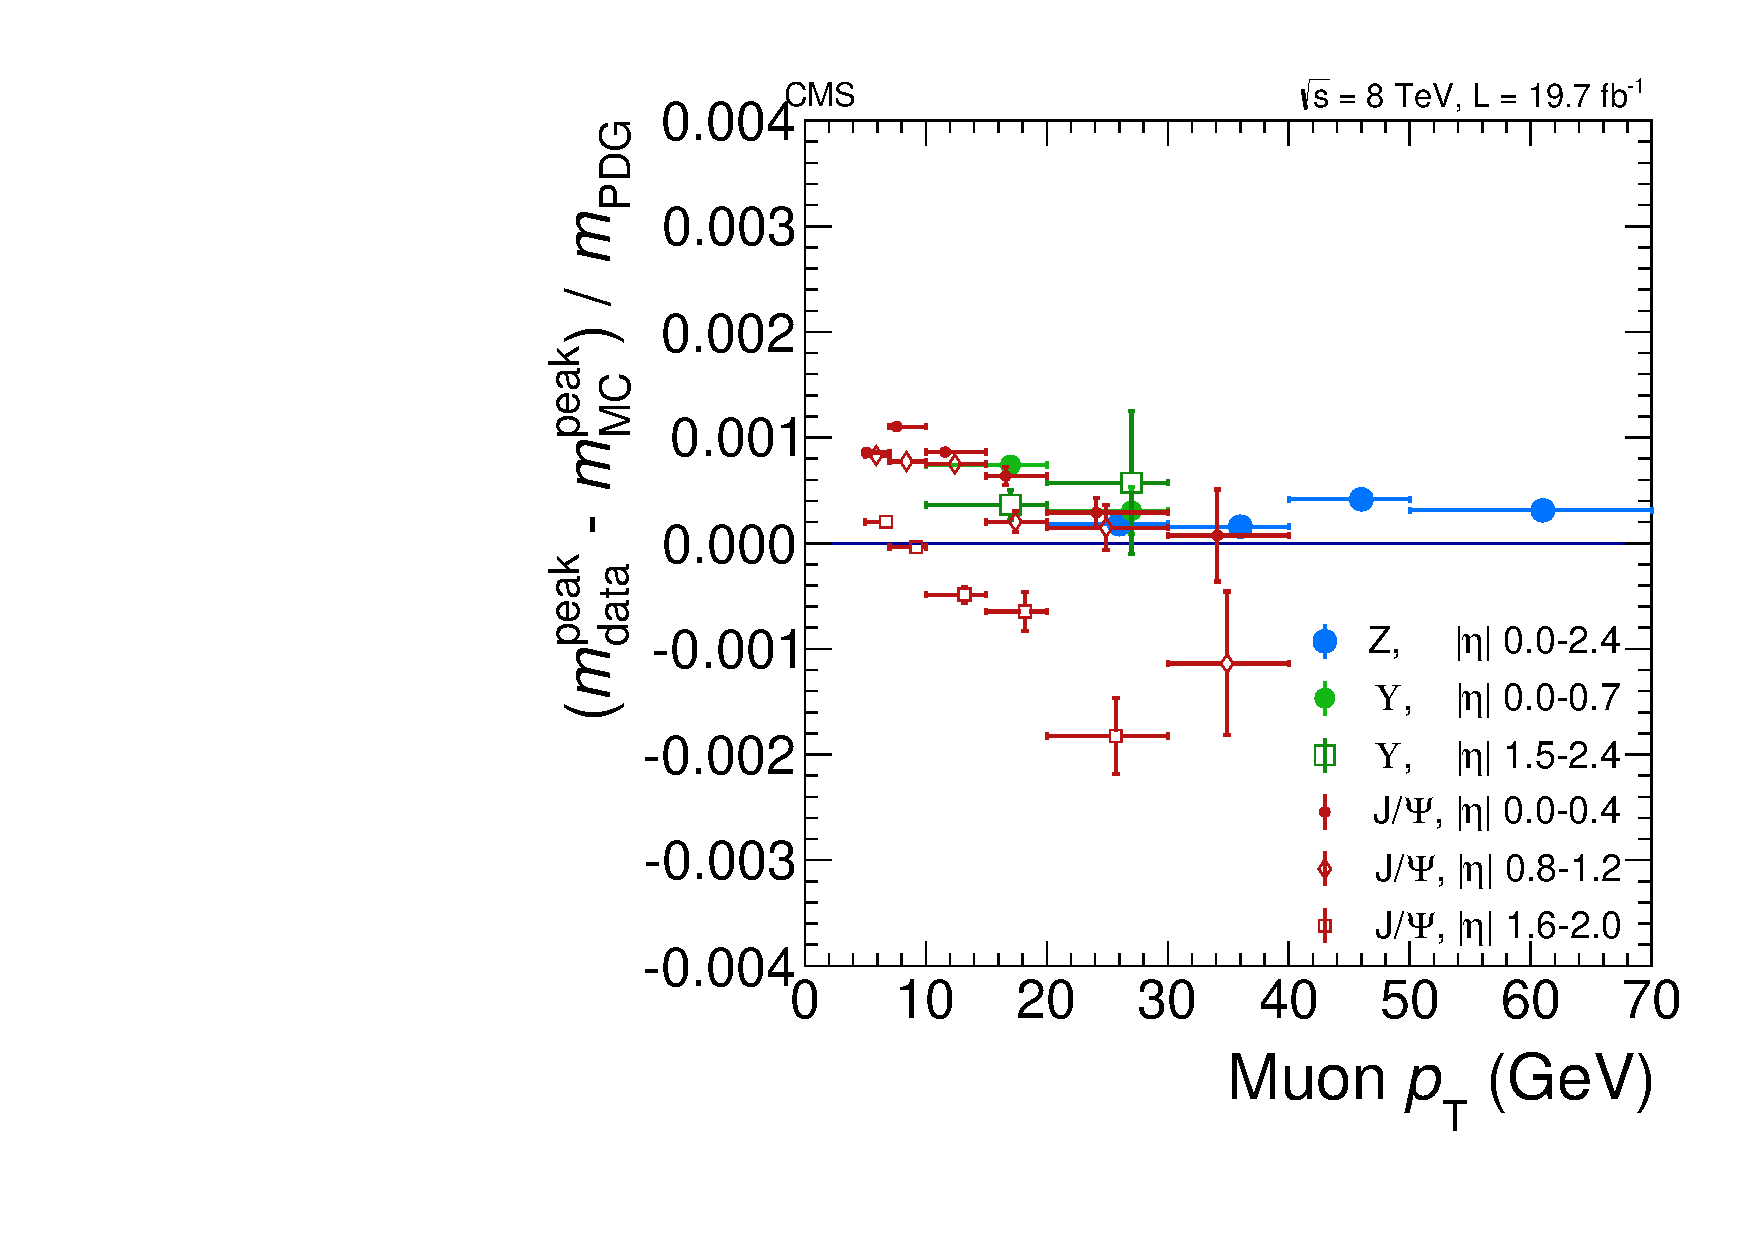
\includegraphics[width=0.45\linewidth]{{LHC_CMS/100_scale_mf}.pdf}
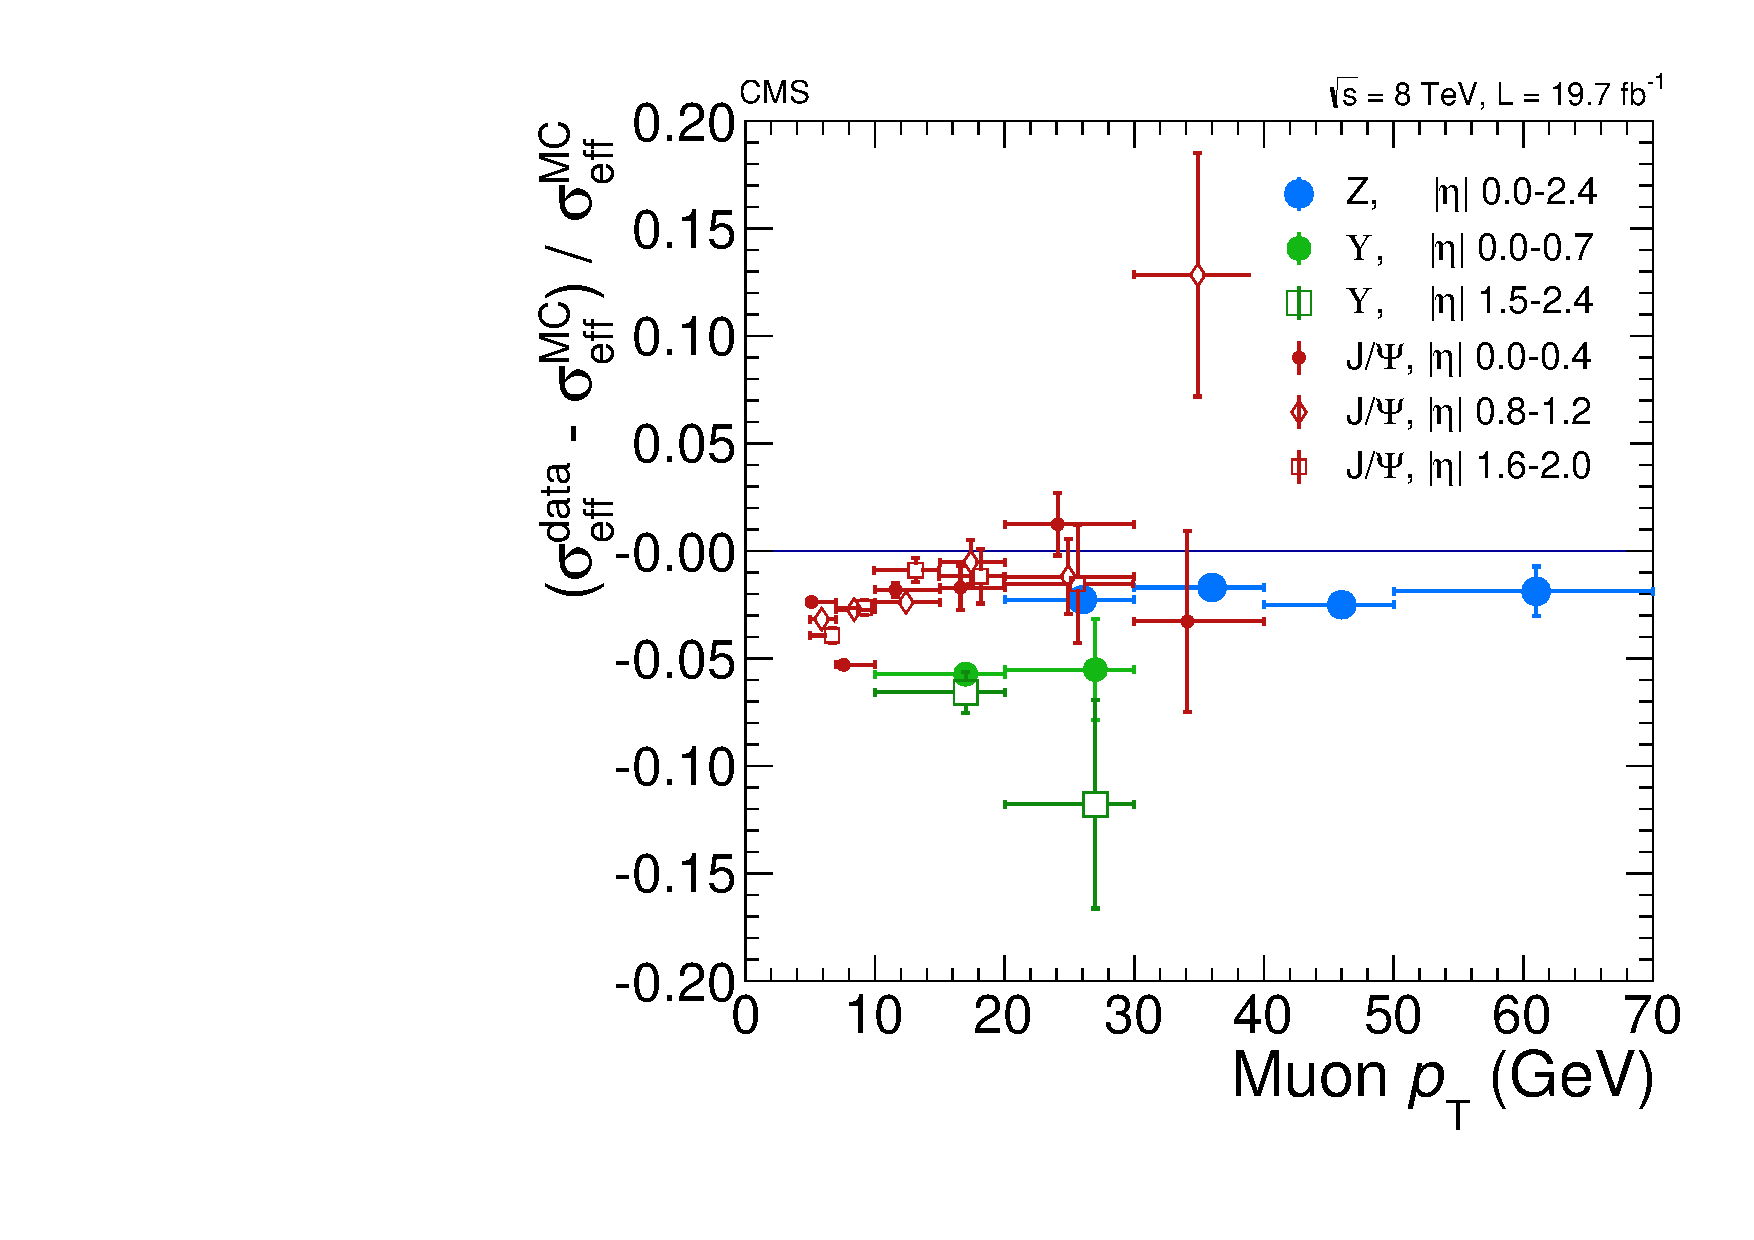
\includegraphics[width=0.45\linewidth]{{LHC_CMS/100_resolution_mf}.pdf}
\caption[(left) Relative difference between the dilepton mass peak positions in data and simulation as obtained from Z, $J/\psi$ and $\Upsilon\left(nS\right)$ resonances as a function of the average muon $p^{\mu}_{T}$ for dimuon events. (right) Relative difference between the dimuon mass resolutions in data and simulation as measured fromZ, $J/\psi$ and $\Upsilon\left(nS\right)$ decays as functions of the average muon]{(left) Relative difference between the dilepton mass peak positions in data and simulation as obtained from Z, $J/\psi$ and $\Upsilon\left(nS\right)$ resonances as a function of the average muon $p^{\mu}_{T}$ for dimuon events. (right) Relative difference between the dimuon mass resolutions in data and simulation as measured fromZ, $J/\psi$ and $\Upsilon\left(nS\right)$ decays as functions of the average muon $p^{\mu}_{T}$\cite{Chatrchyan:2013mxa}.}
\label{fig:Mu_scale_res}
\end{center}
\end{figure}

A Z-boson decay into a lepton pair can be accompanied by final-state radiation, in which case it is desirable to identify and associate the radiated photon to the corresponding lepton to form the Z-boson candidate. Low-energy photons are identified and reconstructed with the PF reconstruction with a dedicated clustering algorithm designed to identify ECAL energy deposits near global muon tracks. Final-state radiated photons are mostly produced with a direction nearly collinear with the parent lepton and have a harder spectrum than background photons from initial-state radiation or pileup interactions. Therefore, to be identified as FSR, a reconstructed photon must be close to the muon they would be associated with and must  make the lepton-pair mass closer to the nominal Z-boson mass. This FSR procedure is applied to muons but not to electrons because the measured electron energies, by construction, already include a large fraction of these photons.

\subsection{Jets}
\label{sec:Jets}

A jet is a narrow cone of hadrons and other particles produced by a quark or gluon as it emanates from a collision. When a quark or gluon is produced in a collision event the vacuum will generate particles and antiparticles because of the effects of QCD. This generates many particles that may leave tracks or energy deposits in the CMS detector. In the analysis the presence of jets is used as an indication of vector-boson fusion (VBF) or associated production with a weak boson, $VH$, with $V = W$ or $Z$, where the $V$ decays hadronically.

In this analysis, jets are reconstructed using the anti-$k_{T}$ clustering algorithm \cite{Cacciari:2008gp}. The inputs to this algorithm are charged hadrons identified by the PF algorithm by matching calorimeter energy clusters to tracks and PF neutral hadrons identified by calorimeter clusters without tracks\footnote{The PF algorithm also has muon and electron pre-identification to omit them from hadron track construction.}. 

The anti-$k_{T}$ algorithm takes these particle tracks and evaluates the distances between particles and combines them into jets by merging together the objects with smallest separation distances. Once a merging has been applied the distances are recalculated and the procedure repeats. The unique part of the anti-$k_{T}$ algorithm is that the distances are inversely weighted by the momentum $\left(k_{T}\right)$ of the particles. This results in low momentum particles clustering with large momentum ones before many low momentum particles cluster with themselves. Figure \ref{fig:anti_kT} shows the jets that result from an example event.

\begin{figure}
\begin{center}
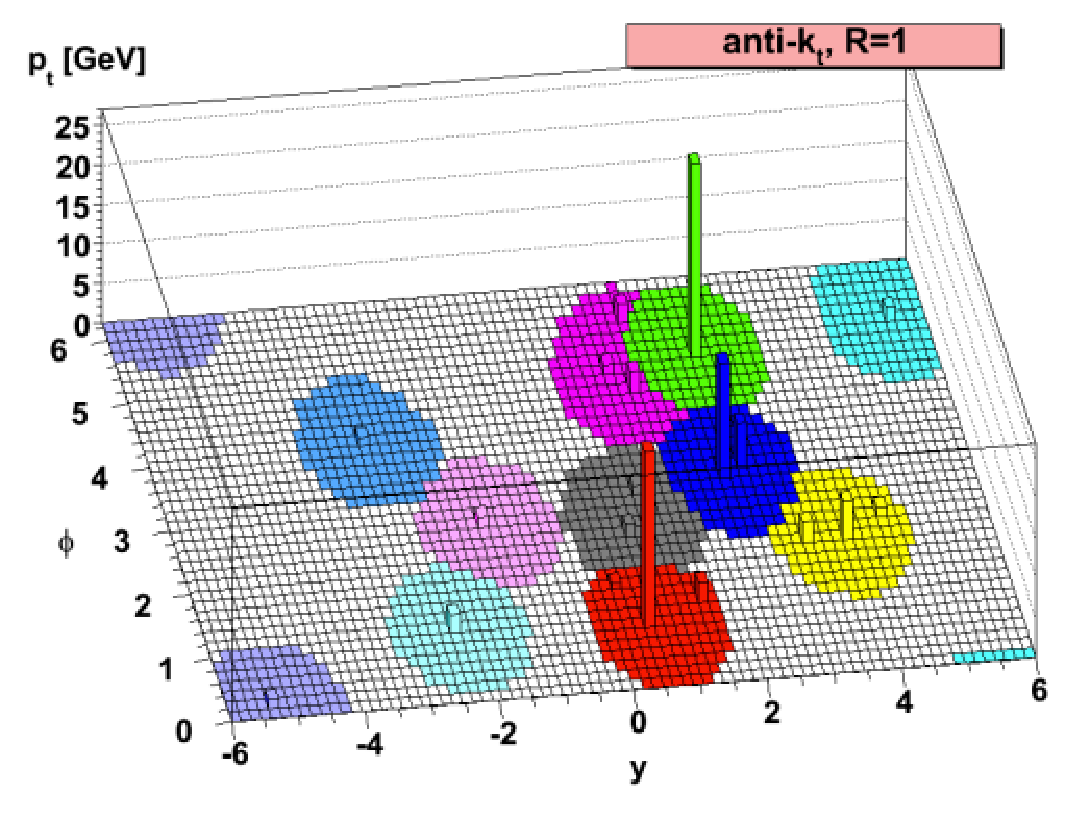
\includegraphics[width=0.45\linewidth]{{LHC_CMS/anti_kT}.pdf}
\caption[An example event of jets formed with the anti-$k_{T}$ clustering algorithm.]{An example event of jets formed with the anti-$k_{T}$ clustering algorithm\cite{Cacciari:2008gp}.}
\label{fig:anti_kT}
\end{center}
\end{figure}

In this analysis jets are only considered if they have $p_{T}^{\text{jet}} > \unit{30}{\GeV}$ and $\abs{\eta^{\text{jet}}} < 4.7$. Corrections and calibrations to the individual components of a jet according to its $p_{T}^{\text{jet}}$ and $\eta^{\text{jet}}$ following \cite{Chatrchyan:2011ds}.

\section{CMS Tracker Alignment}
\label{sec:Alignment}

The precise alignment of the silicon sensors in the CMS Tracker is a necessary and challenging task. While external measurements of the positions of sub-detectors\footnote{Using laser rays for example.} can be a good start, they are woefully inadequate in determining the exact position, tilt angle, and deformation of an individual module. In order to maximize the performance in the complex hardware that is used in the tracker the position of each module must be known to extreme precision. 

The goal of track-based alignment procedures is to determine the module positions from a large sample of reconstructed charge particle trajectories. Each trajectory is built form charge depositions on individual detectors. Using this method, the residual resolution is now below $\unit{10}{\micro\meter}$ \cite{Bayatian:922757}. This optimization problem can be formulated in the context of linear least squares. Module position corrections $\mathbf{p}$ are determined by minimizing an objective function

\begin{equation}
\label{eq:alignment}
\chi^{2}\left(\mathbf{p},\mathbf{q}\right) = \sum_{j}^{\text{tracks}}\sum_{i}^{\text{hits}}\mathbf{r}_{ij}^{T}\left(\mathbf{p},\mathbf{q}_{j}\right)\mathbf{V}_{ij}^{-1}\mathbf{r}_{ij}\left(\mathbf{p},\mathbf{q}_{j}\right),
\end{equation}

which can be expressed as a sum over all hits $i$ on all tracks $j$ and track parameters $\mathbf{q}_{j}$, assuming negligible correlations between hits. Track residuals $\mathbf{r}_{ij} = \mathbf{m}_{ij} - \mathbf{f}_{ij}\left(\mathbf{p},\mathbf{q}_{j}\right)$ are defined as the difference between the measured hit position and the estimated impact point from the trajectory without the hit in question. These residuals are given as either one- or two-dimensional vectors, and $\mathbf{V}_{ij}$ is either the squared error or the covariance matrix respectively\cite{Chatrchyan:2009sr}.

In order to determine the 200000 different parameters, \textit{alignment parameters}, that describe the locations of the 1440 silicon pixel and 15148 silicon microstrip modules two methods of minimizing track residuals are used, {\sf MILLEPEDE II} and {\sf HIP}. A \textit{track} is a fit to the series of consecutive signals that a charged particle will leave in each layer of silicon as it passes through the CMS tracker. Each of the two algorithms minimizes the residual difference between the hits that make up a track and the position of the track created without that hit. 

The main difference between the two algorithms lies in how this minimization is done. {\sf MILLEPEDE II} simultaneously determines the solutions of a complete matrix equation for global and local parameters using all tracks \cite{Blobel:2002ax}. {\sf HIP}, Hit and Impact Point, determines these parameters iteratively to solve for correlations between modules. The algorithm repeatedly fits a track and then changes a parameter, eventually minimizing the $\chi^2$ for the fit \cite{Karimaki:2006az}.

Vital to the work done as part of this thesis is the connection between the global and local parameters. The tracks and hits are defined on the module level. However these modules are connected to each other and to other subdetectors through mechanical structures that can be used to constrain the system for minimization. In figures \ref{fig:Pix_strct} and \ref{fig:Strip_strct} we map the different structures that can are used to define the locations and constraints that should be used for a given track. 


\begin{figure}
\begin{center}
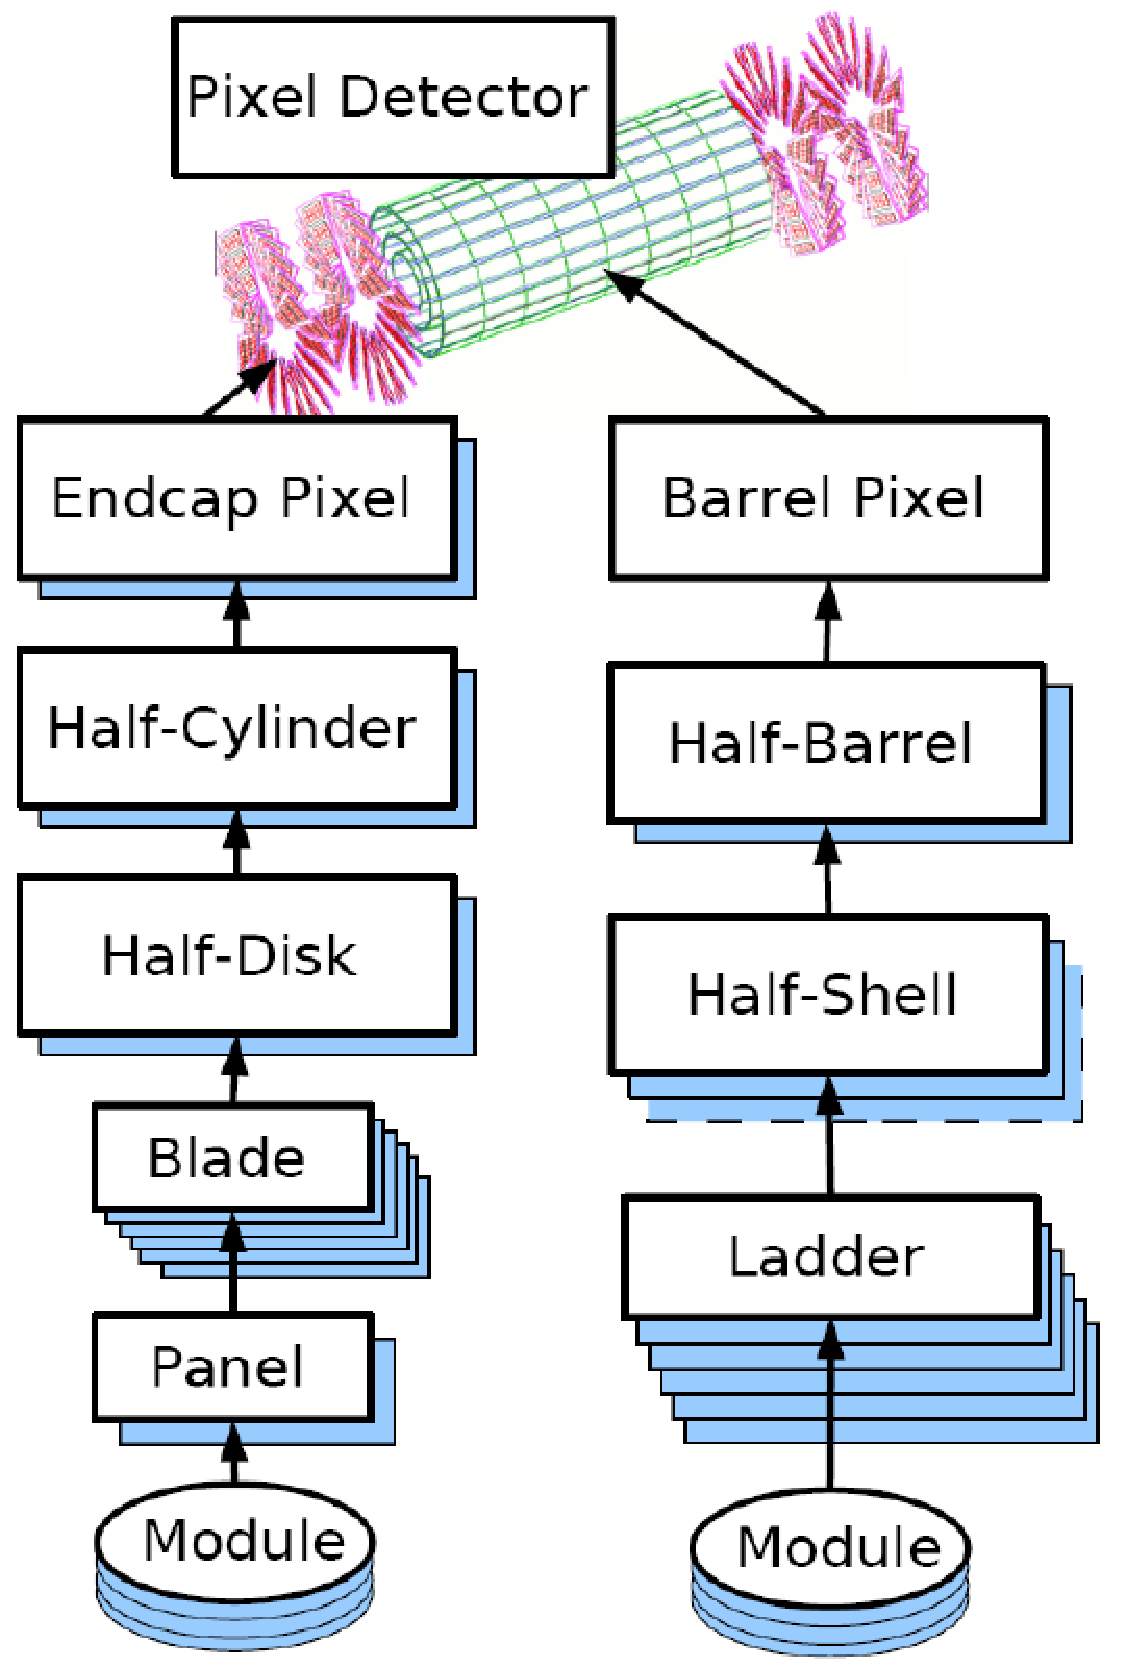
\includegraphics[width=0.45\linewidth]{{LHC_CMS/Pix_strct}.pdf}
\caption[Hierarchy of the CMS silicon pixel detector structures.]{Hierarchy of the CMS silicon pixel detector structures\cite{CMS-doc-1157-v7}.}
\label{fig:Pix_strct}
\end{center}
\end{figure}

\begin{figure}
\begin{center}
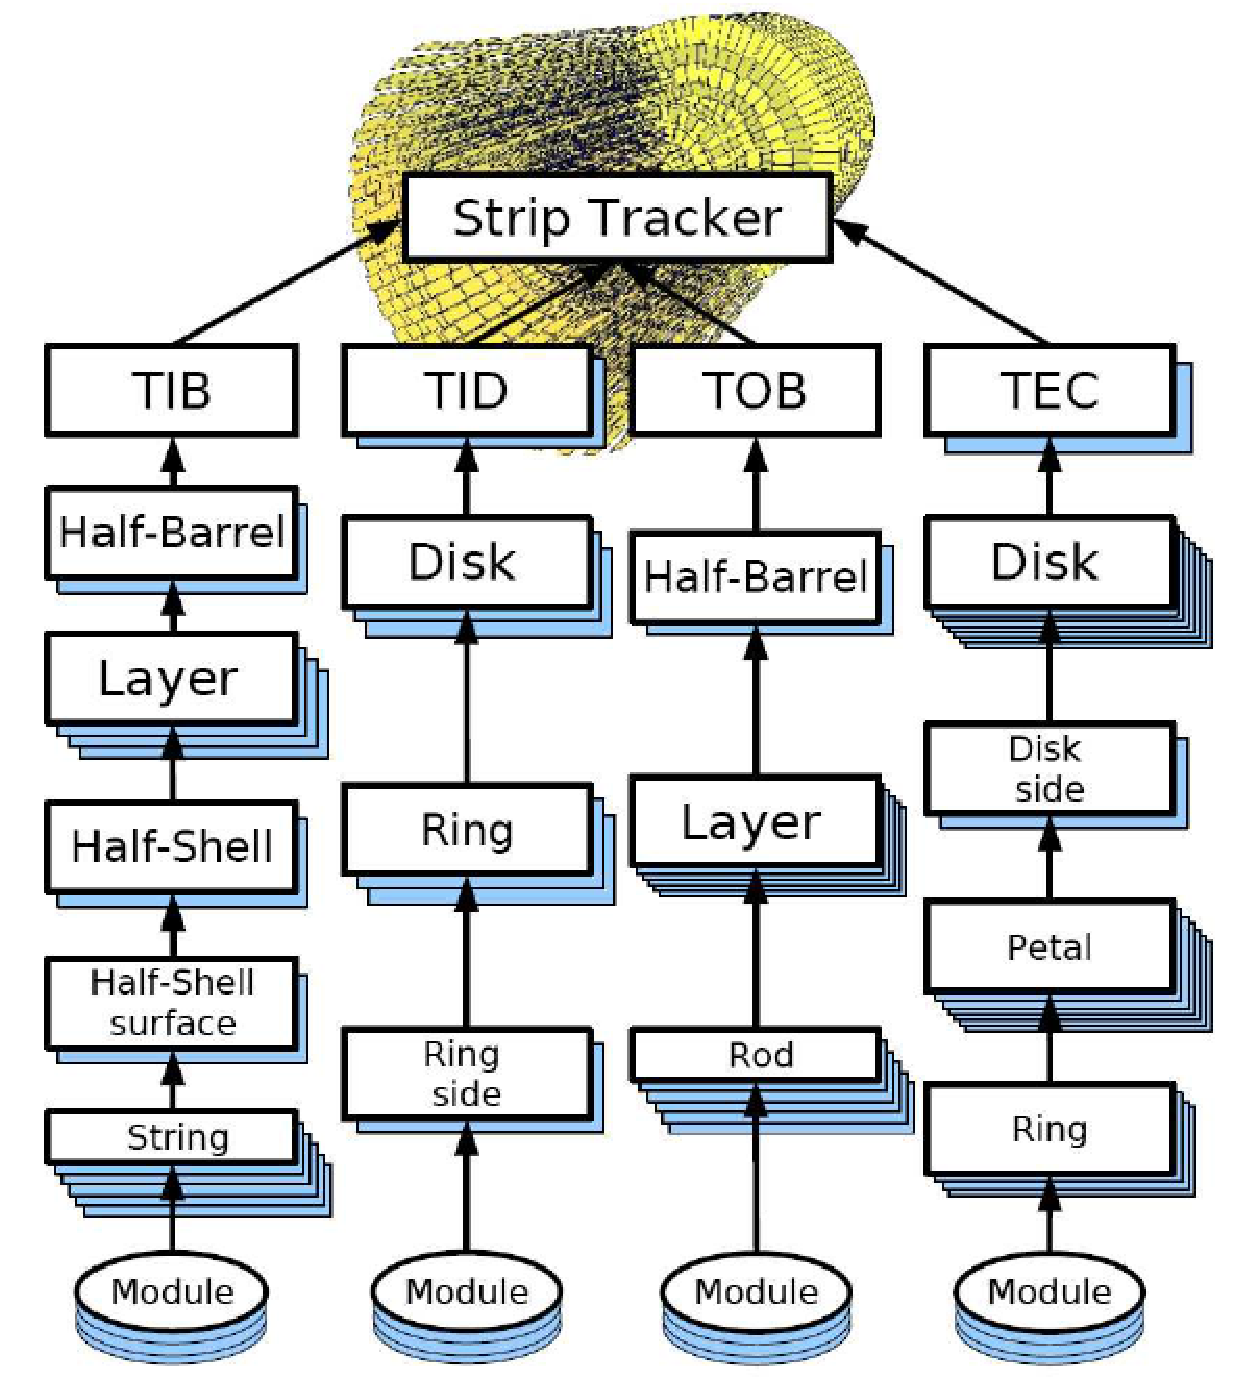
\includegraphics[width=0.45\linewidth]{{LHC_CMS/Strip_strct}.pdf}
\caption[Hierarchy of the CMS silicon strip detector structures.]{Hierarchy of the CMS silicon strip detector structures\cite{Adam:2009aa}.}
\label{fig:Strip_strct}
\end{center}
\end{figure}

\subsection{Silicon Pixel Alignment in Prompt Calibration Loop}
Once a set of alignment parameters is determined, it is not valid forever. As the detector operates the different components may shift. A prime example of this is the pixel barrel, which is not in a fixed position. This is problematic because the CMS magnet may turn on and off, resulting in natural shifts in the positions of different detectors. Part of this thesis work was to develop and implement an active alignment algorithm that would detect and automatically update the detector positions as the CMS experiment takes data.

This active alignment algorithm was implemented in the CMS tracker Prompt Calibration Loop for the start of the 2015 run of the LHC. The Prompt Calibration Loop is a collection of routines that are designed to monitor and automatically adjust parameters to optimize the performance of the the CMS tracking system. The alignment routine developed during this thesis work monitors and adjusts the 36 alignment parameters that describe the pixel detector global parameters. The monitored parameters are the positions $\left(x, y, z\right)$ and rotations $\left(\theta_{x}, \theta_{y}, \theta_{z}\right)$ of the two BPIX half-barrels and the four half-cylinders of the FPIX system\footnote{Two half-cylinders each for FPIX+ and FPIX-.}. If a sufficient shift in one of these parameters is seen\footnote{In this case, ``sufficient" implies the parameter shifts between a pre-set minimum and maximum window and the significance of that shift is larger than a pre-set amount.} then the database of tracker conditions is updated. These consistent updates allow CMS to continue operating at peak performance and avoids rerunning computationally expensive data processing routines to correct the data after the fact. 

The effectiveness of this project is illustrated from similar algorithm that was used at the end of the 2012 run after a large shift in the pixel barrel position was seen. Figure \ref{fig:2011PixelShift} shows the longitudinal shift between the two half-shelf of the BPIX as measured with the primary vertex residuals. The previous monitoring procedure was implemented farther `downstream' in the computing chain than the current implementation.

\begin{figure}
\begin{center}
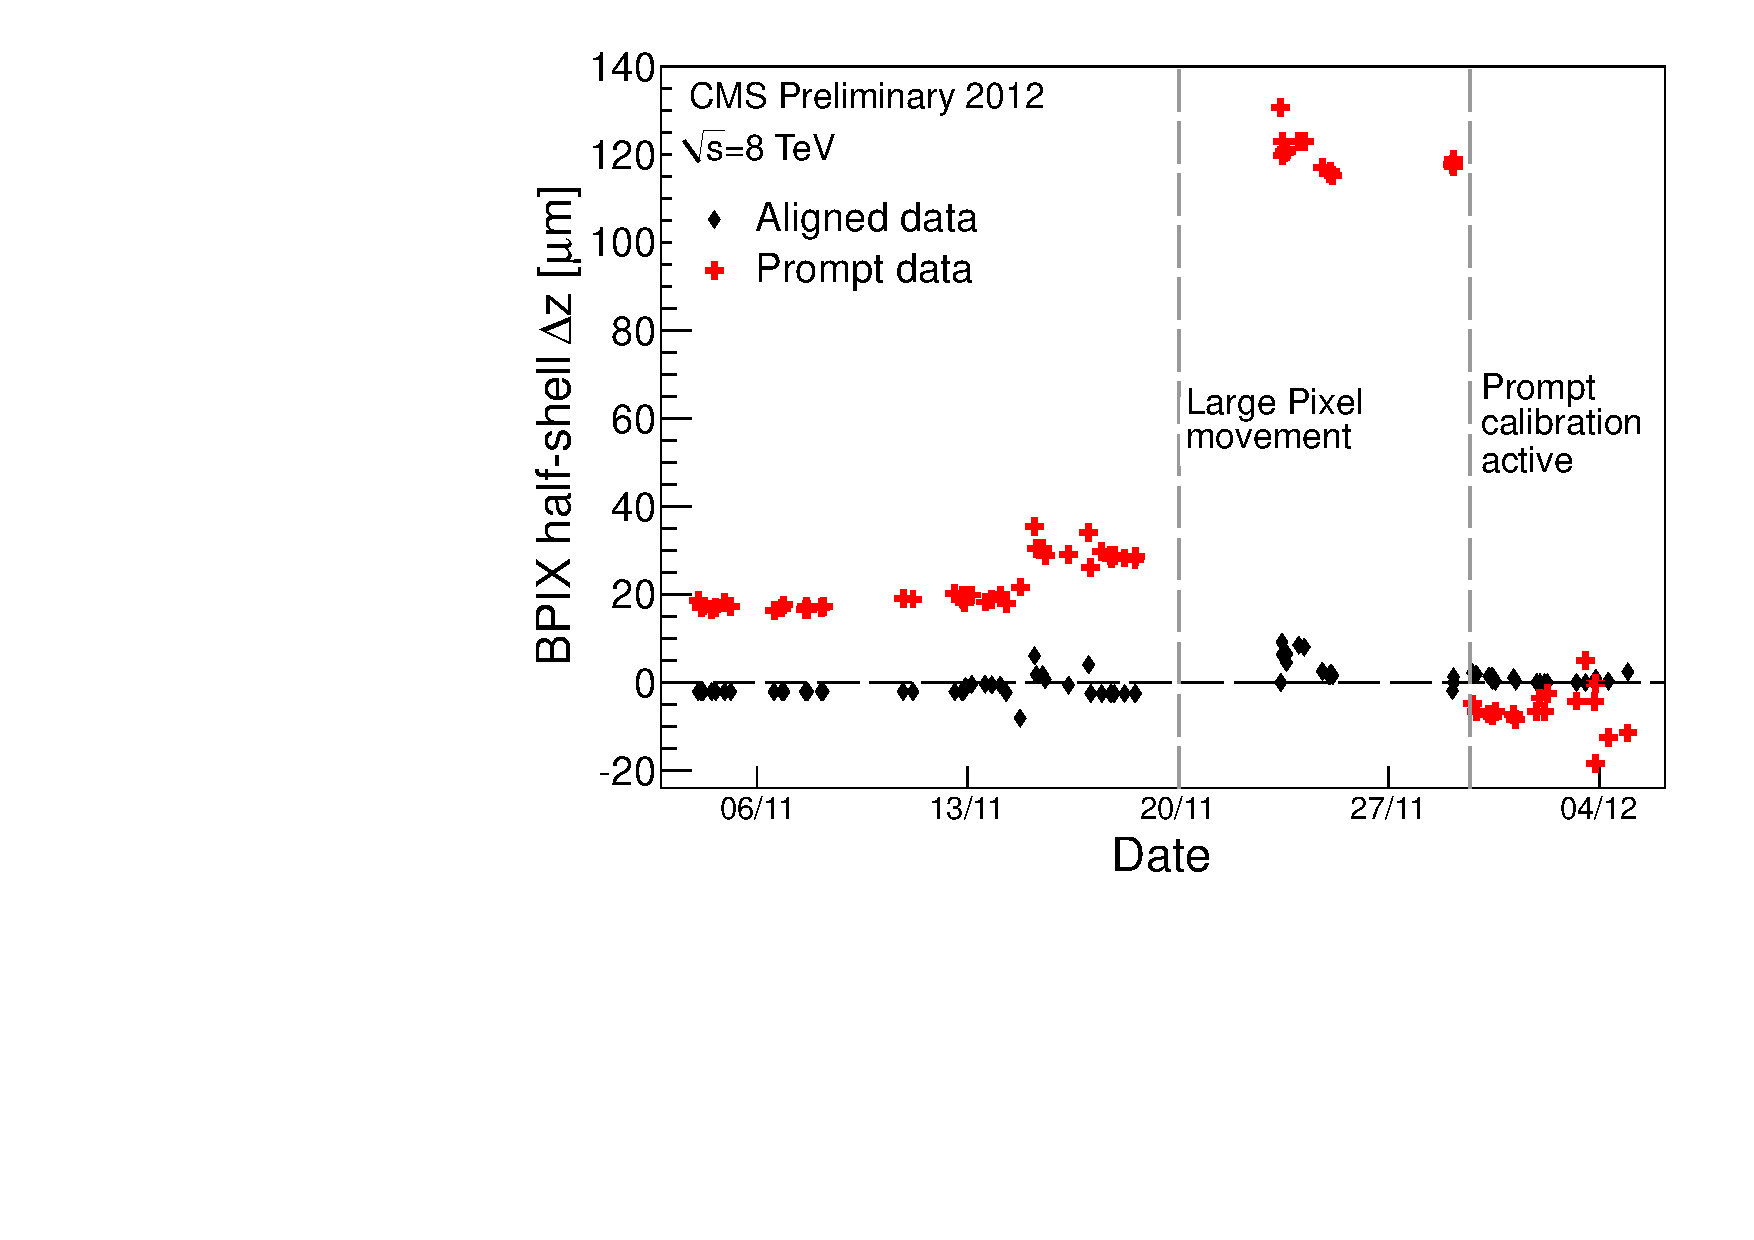
\includegraphics[width=.65\linewidth]{{LHC_CMS/PCL_lateNovRuns}.pdf}
\caption[Day-by-day value of the relative longitudinal shift between the two half-shells of the BPIX as measured with the primary vertex residuals, for the last month of pp data taking in 2012. Red crosses show the shift observed using the data coming from the prompt reconstruction. The same events, re-reconstructed after the 2012 alignment campaign, which accounts for the major changes in the positions of the half-shells, are represented by black lozenges. A major displacement of the half-shells O(100) $\micro\meter$, occurred during the technical stop in the week of 20th of November, is recovered by the prompt alignment of the BPIX large structures that became active on the 30th November.]{Day-by-day value of the relative longitudinal shift between the two half-shells of the BPIX as measured with the primary vertex residuals, for the last month of pp data taking in 2012. Red crosses show the shift observed using the data coming from the prompt reconstruction. The same events, re-reconstructed after the 2012 alignment campaign, which accounts for the major changes in the positions of the half-shells, are represented by black lozenges. A major displacement of the half-shells O(100) $\micro\meter$, occurred during the technical stop in the week of 20th of November, is recovered by the prompt alignment of the BPIX large structures that became active on the 30th November \cite{CMS-DP-2013-017}.}
\label{fig:2011PixelShift}
\end{center}
\end{figure}

\chapter{Higgs boson at the LHC: Phenomenology}
\label{sec:LHC_Pheno}
\chaptermark{Higgs boson at the LHC: Phenomenology}


In this section we discuss specific phenomenological details that are studied for this thesis. First, we discuss the different modes of producing a Higgs boson at the LHC, and different features of these different production modes. Next, we will present the decay of a Higgs boson into two Z bosons and subsequently four leptons. Using this information we will present the implications of off resonance production and decay on the Higgs boson lifetime. Finally, we will discuss the spin and parity of a single-produced resonance and how we can use these relations to characterize a new particle found at the LHC.

\section{Higgs boson production at LHC}
\label{sec:Higgs_Production_Pheno}

In proton-proton collisions a SM Higgs boson can be produced through the coupling of a Higgs boson to either bosons or fermions. Each of these two categories of Higgs boson production will be dominated by specific production modes. Fermionic production of a Higgs boson can happen either through \textit{gluon-gluon fusion} $gg \to H$ (ggH) and much less frequently through production in \textit{association with two top quarks} $gg \to H + t\bar{t}$ ($t\bar{t}H$). Bosonic production of a Higgs boson can occur through \textit{vector boson fusion} (VBF), where two quarks radiate vector bosons which produce the boson in association with two quark jets $qq \to H + 2\text{jets}$ or through production \textit{associated with a vector boson} $qq \to H + W/Z$ (VH).

The cross sections of these different production mechanisms as a function of the Higgs boson mass at the LHC are shown in figure \ref{fig:LHC_Hxsec} for the two center of mass energies used in this thesis; $\sqrt{s} = \unit{7}{\TeV}$ and $\sqrt{s} = \unit{8}{\TeV}$ \cite{Dittmaier:2011ti, Dittmaier:2012vm}. Notable features of these cross sections are the order of magnitude difference between gluon-gluon fusion and the bosonic production modes which are all much larger than the $H + t\bar{t}$ production. Additionally, one can see the boost in the gluon-gluon fusion production at $2m_{t}$, which corresponds to the top quark in the production loop going becoming on shell (explained in more detail below).

\begin{figure}
\begin{center}
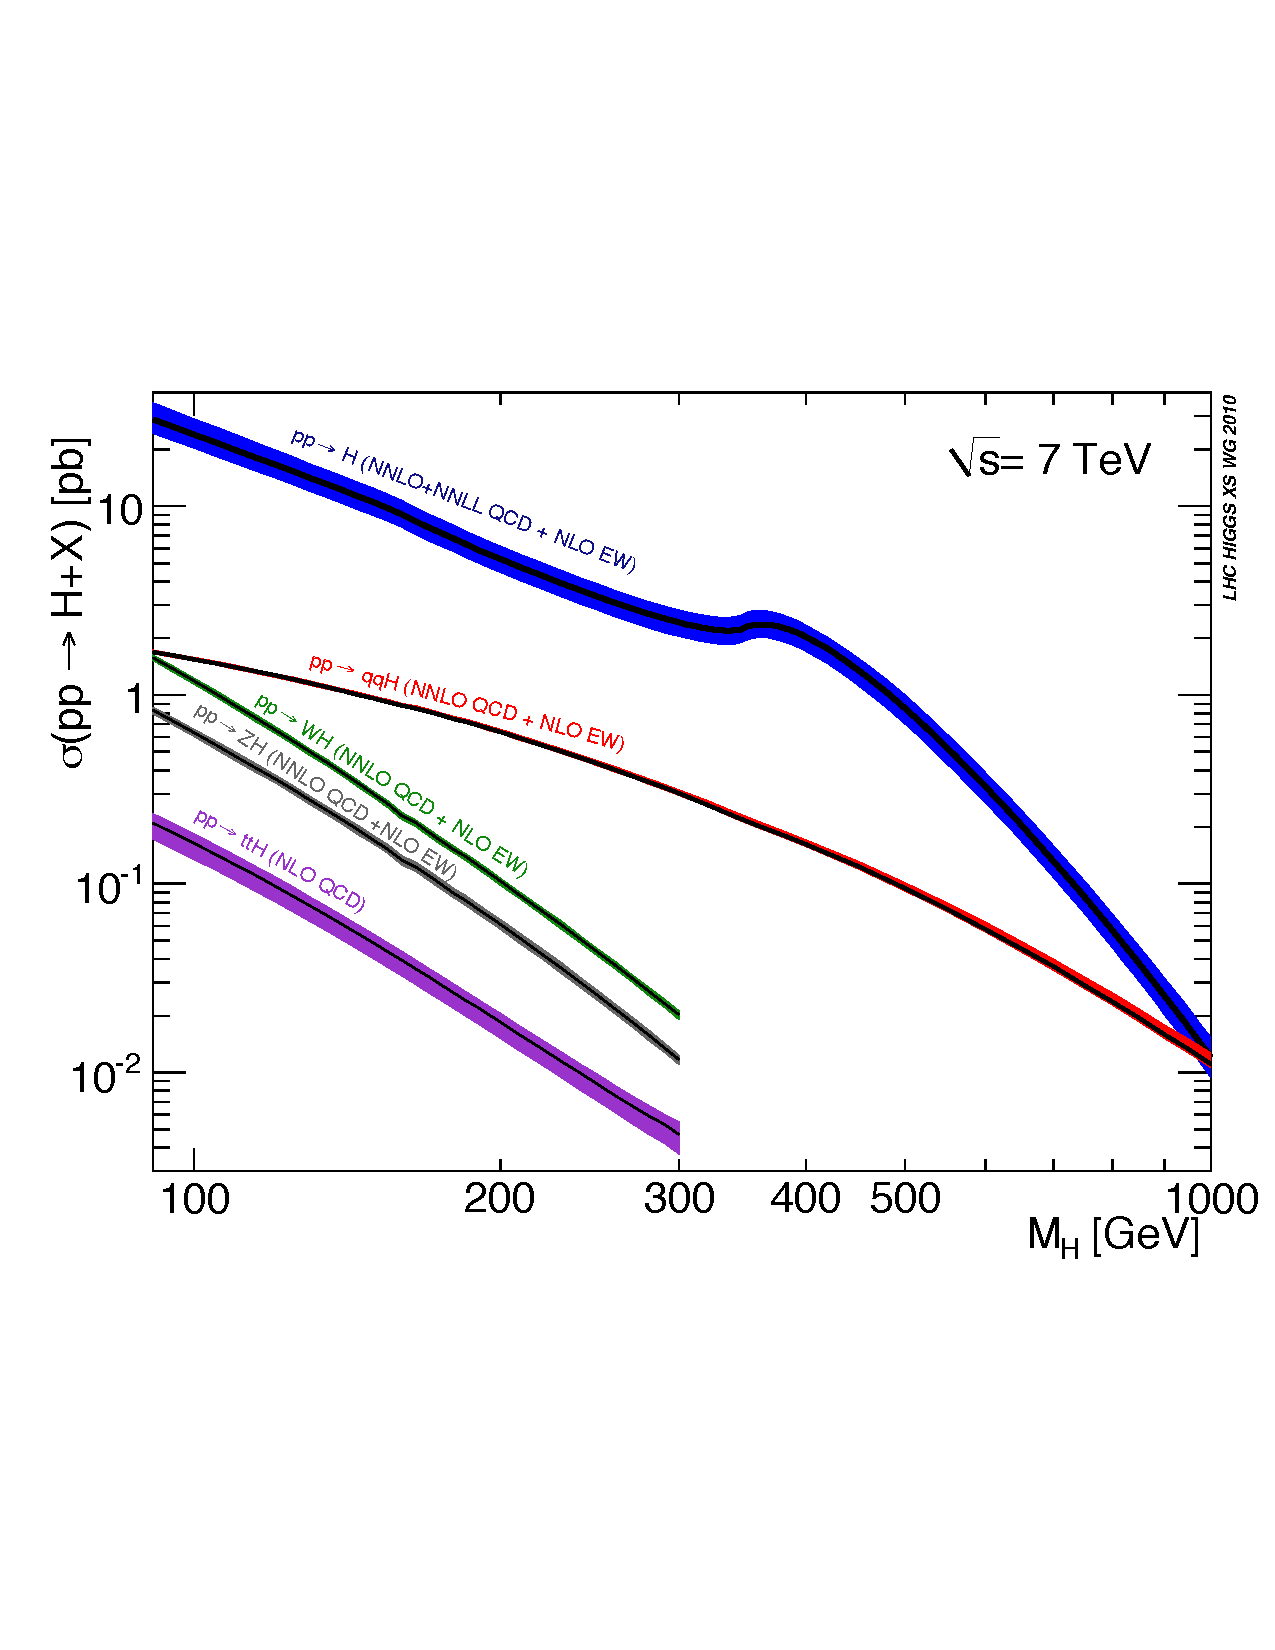
\includegraphics[width=0.46\linewidth]{{LHC_Pheno/Higgs_XS_7TeV}.pdf}
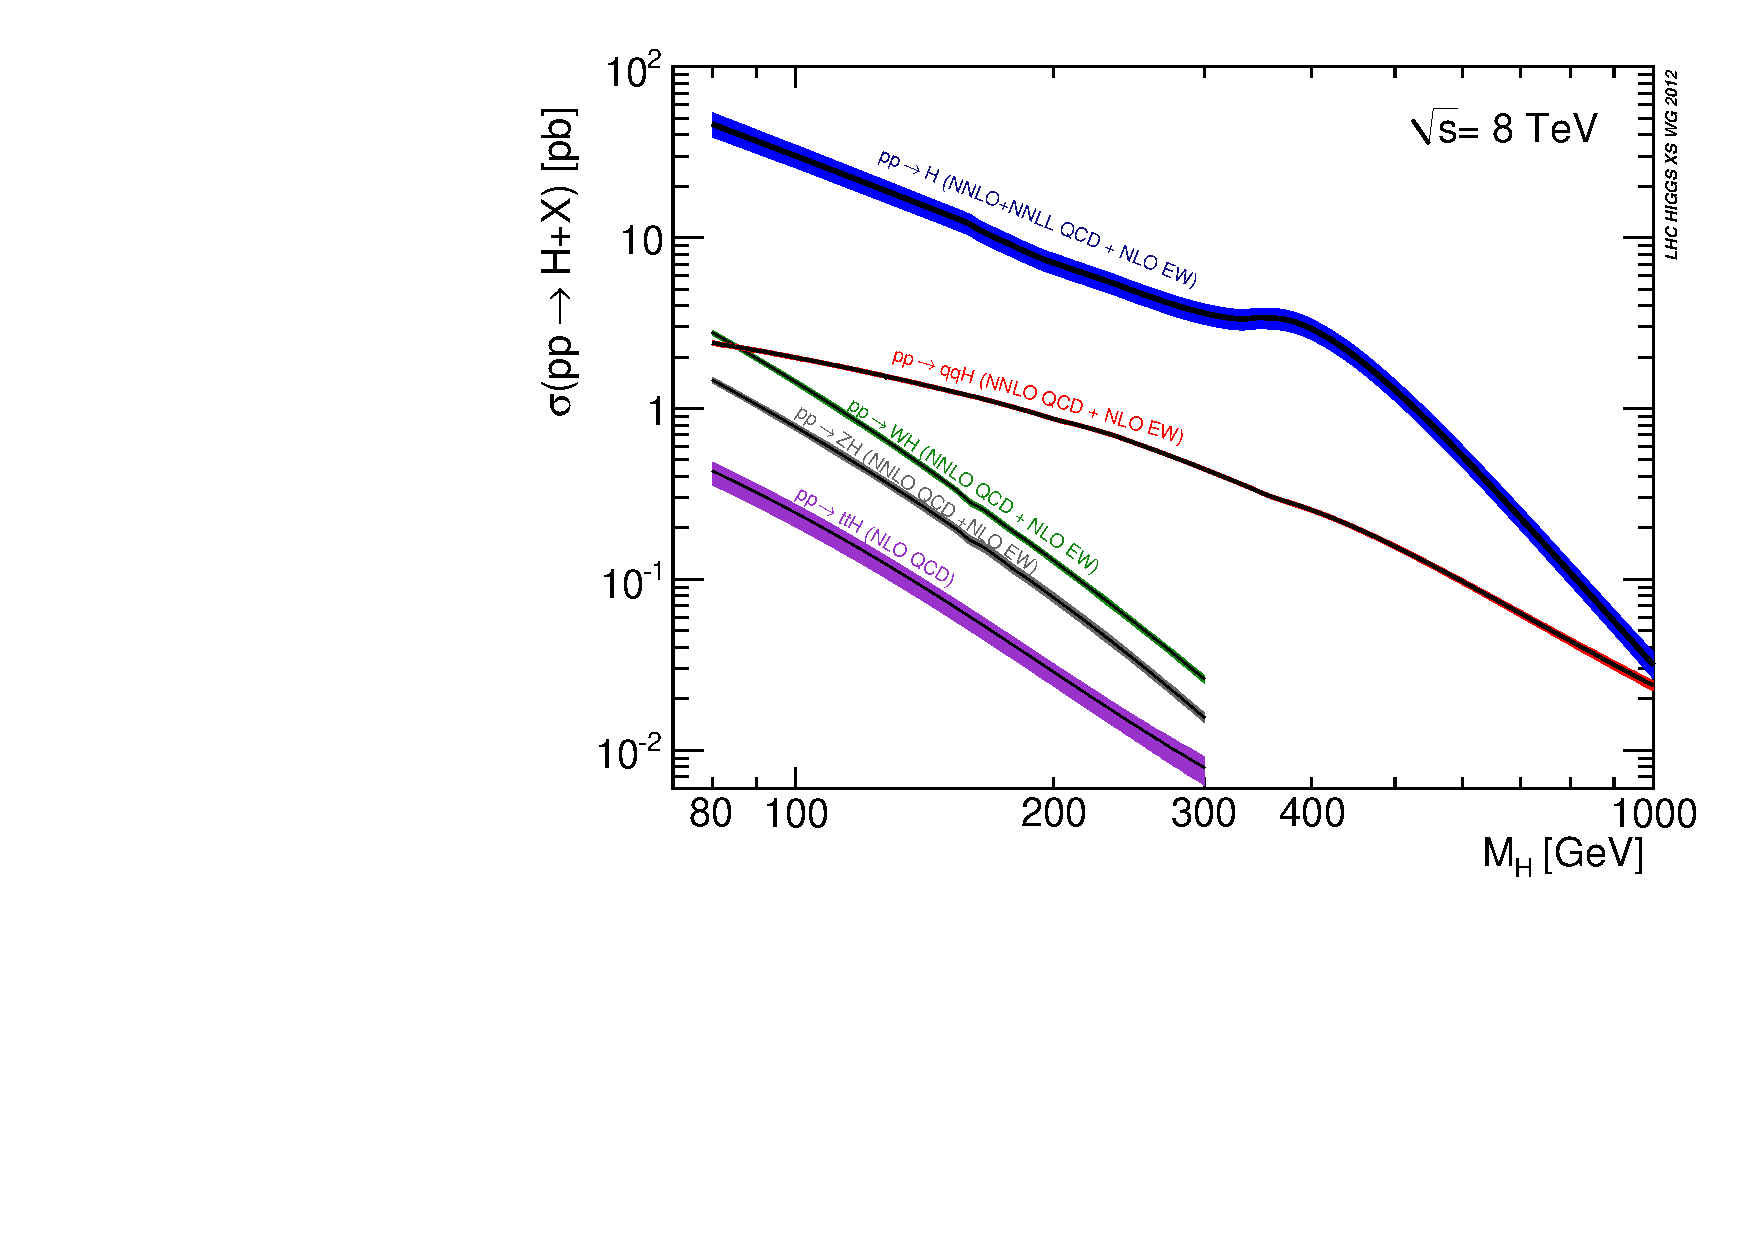
\includegraphics[width=0.455\linewidth]{{LHC_Pheno/Higgs_XS_8TeV_lx}.pdf}
\caption[Standard Model Higgs boson production cross sections and relative uncertainties at $\sqrt{s} = \unit{7}{\TeV}$ and $\sqrt{s} = \unit{8}{\TeV}$. From top to bottom these are $pp \to H$, blue, $pp \to H + 2\text{jets}$, red, $pp \to H + W$, green, $pp \to H + Z$, grey, $pp \to H + t\bar{t}$, purple.]{Standard Model Higgs boson production cross sections and relative uncertainties at $\sqrt{s} = \unit{7}{\TeV}$ and $\sqrt{s} = \unit{8}{\TeV}$. From top to bottom these are $pp \to H$, blue, $pp \to H + 2\text{jets}$, red, $pp \to H + W$, green, $pp \to H + Z$, grey, $pp \to H + t\bar{t}$, purple \cite{Dittmaier:2011ti, Dittmaier:2012vm}.}
\label{fig:LHC_Hxsec}
\end{center}
\end{figure}

The main production mechanism at the LHC is gluon-gluon fusion. The Feynman diagram for this process is shown in figure \ref{fig:ggH_Feyn}. While the Higgs boson does not couple directly to gluons (because they are massless) this mode of production relies on the Higgs boson coupling to fermions generated by the incoming gluons. Because the coupling of the Higgs boson is proportional to the mass of the fermion the dominant contribution is the Higgs boson -- top coupling. This leads to a boost in the cross section when the mass of the Higgs boson is twice the top mass because the top in the loop shown is no longer virtual. For the entire mass range that is considered in this analysis this is the most common way to produce a Higgs boson at the LHC.

\begin{figure}
\begin{center}
\unitlength=1mm
\begin{fmffile}{ggH_Feyn}

\begin{fmfgraph*}(40,30) 
  \fmfleft{i1,i2} \fmfright{sp1}
  \fmf{gluon,label=$g$}{i1,v1} 
  \fmf{gluon,label=$g$}{i2,v2}
  \fmf{fermion}{v1,v2,v3,v1}
  \fmffixed{(0,.6h)}{v1,v2}
  \fmf{dashes,label=$H$}{v3,sp1}
\end{fmfgraph*}

\end{fmffile}
\end{center}
\caption[Feynman diagram depicting Higgs boson production through gluon-gluon fusion $gg \to H$. The fermion loop is dominated by top quarks, however all quarks contribute according to their masses.]{Feynman diagram depicting Higgs boson production through gluon-gluon fusion $gg \to H$. The fermion loop is dominated by top quarks, however all quarks contribute according to their masses.}
\label{fig:ggH_Feyn}
\end{figure}

The second most likely way to produce a Higgs boson at the LHC is through vector boson fusion. To produce a Higgs boson this way two quarks each radiate a W or Z boson which fuse into the Higgs boson. This production mode relies on the Higgs boson coupling to the vector bosons, making it distinct compared to gluon-gluon fusion. the distinguishing feature of this production mode is the presence of two quark jets in the final state in addition to the Higgs boson. These jets contain information about the Higgs boson and can be exploited to refine searches and study the properties of a new particle. The Feynman diagram for this process is shown in figure \ref{fig:qqH_Feyn}.

\begin{figure}
\begin{center}
\unitlength=1mm
\begin{fmffile}{qqH_Feyn}

\begin{fmfgraph*}(40,30) 
  \fmfleft{i1,i2} \fmfright{sp1,sp2,sp3}
  \fmf{fermion,label=$q$}{i1,v1,sp1} 
  \fmf{fermion,label=$q$}{i2,v2,sp3}
  \fmf{boson,label=$W/Z$,label.side=left}{v1,v3}
  \fmf{boson}{v3,v2}
  \fmffixed{(0,.3h)}{v1,v3}
  \fmffixed{(0,.3h)}{v3,v2}
  \fmf{dashes,label=$H$}{v3,sp2}
\end{fmfgraph*}

\end{fmffile}
\end{center}
\caption[Feynman diagram depicting Higgs boson production through vector boson fusion $qq \to H + 2\text{jets}$.]{Feynman diagram depicting Higgs boson production through vector boson fusion $qq \to H + 2\text{jets}$.}
\label{fig:qqH_Feyn}
\end{figure}

Sub-dominant to these two production modes are processes that produce a Higgs boson in association with vector bosons or top quarks. This thesis does not tune the analysis to separate these modes from the dominant ones, instead they are grouped with the dominant modes by how the Higgs boson couples to the other standard model particles. VBF is grouped with VH because the Higgs boson is produced through a coupling to vector bosons while $t\bar{t}H$ is grouped with ggH because it relies on the Higgs boson coupling to fermions.

Producing the Higgs boson in association with a W or Z boson is conceptually similar to VBF production. Two quarks interact, producing a vector boson which radiates away a Higgs boson, shown in figure \ref{fig:VH_Feyn}. Unique to this final state is that in addition to the Higgs boson you will also have the particles associated with the subsequent decay of a W or Z boson. The $t\bar{t}H$ production mode is the smallest of those considered here and is similar to ggH in that it relies on the Higgs boson coupling to top quarks. While the rates of $t\bar{t}H$ are very low, Higgs bosons produced in this way can be distinguished by the presence of two top quarks in addition to the decay product of the Higgs boson, as shown in figure \ref{fig:ttH_Feyn}.

\begin{figure}
\begin{center}
\unitlength=1mm
\begin{fmffile}{VH_Feyn}

\begin{fmfgraph*}(40,30) 
  \fmfleft{i1,i2} \fmfright{sp1,sp2}
  \fmf{fermion,label=$q$}{i1,v1,i2} 
  \fmf{boson}{v1,v3}
  \fmf{boson,label=$W/Z$}{v3,sp1}
  \fmffixed{(.3w,0)}{v1,v3}
  \fmf{dashes,label=$H$}{v3,sp2}
\end{fmfgraph*}

\end{fmffile}
\end{center}
\caption[Feynman diagram depicting Higgs boson production associated with a vector boson $qq \to H + W/Z$.]{Feynman diagram depicting Higgs boson production associated with a vector boson $qq \to H + W/Z$.}
\label{fig:VH_Feyn}
\end{figure}

\begin{figure}
\begin{center}
\unitlength=1mm
\begin{fmffile}{ttH_Feyn}

\begin{fmfgraph*}(40,30) 
  \fmfleft{i1,i2} \fmfright{sp1,sp2,sp3}
  \fmf{gluon,label=$g$}{i1,v1} 
  \fmf{gluon,label=$g$}{i2,v2}
  \fmf{fermion,label=$t$}{sp1,v1}
  \fmf{fermion}{v1,v3,v2}
  \fmf{fermion,label=$t$}{v2,sp3}
  \fmffixed{(0,.3h)}{v1,v3}
  \fmffixed{(0,.3h)}{v3,v2}
  \fmf{dashes,label=$H$}{v3,sp2}
\end{fmfgraph*}

\end{fmffile}
\end{center}
\caption[Feynman diagram depicting Higgs boson production in association with two top quarks $gg \to H + t\bar{t}$.]{Feynman diagram depicting Higgs boson production in association with two top quarks $gg \to H + t\bar{t}$.}
\label{fig:ttH_Feyn}
\end{figure}

More details are presented in section \ref{sec:prod_dec_frac}, this thesis uses the different properties of ggH and VBF production modes to measure how often a Higgs boson is produced in each mode at the LHC. This work resulted in the first measurement of the production mechanism of Higgs bosons in the $4\ell$ final state.

\section{Higgs boson decay to \texorpdfstring{$ZZ \to 4\ell$}{ZZ to 4l}}
\label{sec:Higgs_Decay_ZZ_4l}

The SM Higgs boson is an unstable particle that will decay before it can be detected with the CMS detector. However, we can search for this particle by looking at its decay products. To determine which decay products will be the most fruitful to use for a search, we look at the \textit{branching ratio} $BR_{X} = \frac{N_{X}}{N_{tot}}$ of the Higgs boson decay for a specific final state in relation to the total number of Higgs bosons we expect. Thus, a high branching ratio will result in a larger number of signal events. In figure \ref{fig:Higgs_BR} we plot some of the interesting branching ratios as a function of the Higgs boson mass. To decide if a search is valuable we compare the number of events we expect from a specific decay mode (given by the luminosity times branching ratio times the cross section $\mathcal{L}\cdot BR_{X}\cdot\sigma_{tot}$) to the number of background events we expect in the search range.

\begin{figure}
\begin{center}
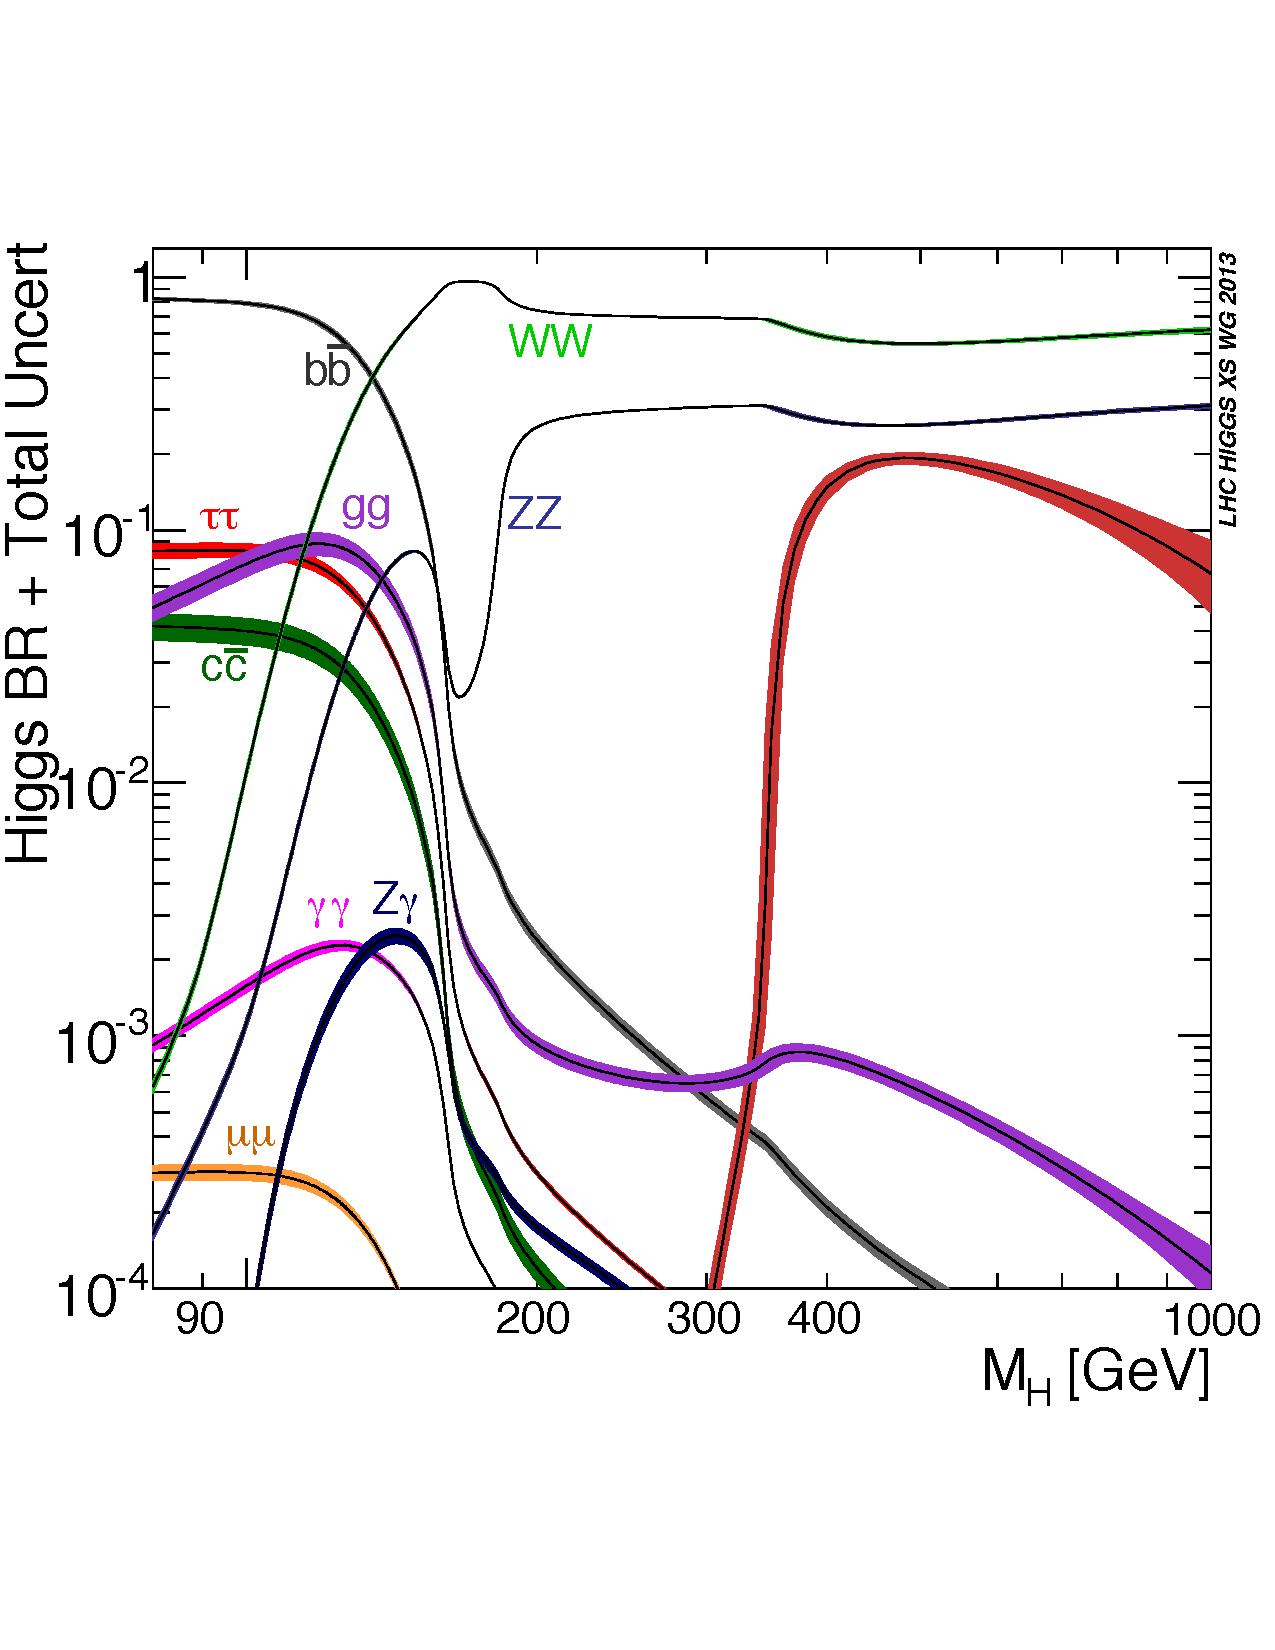
\includegraphics[width=0.45\linewidth]{{LHC_Pheno/Higgs_BR}.pdf}
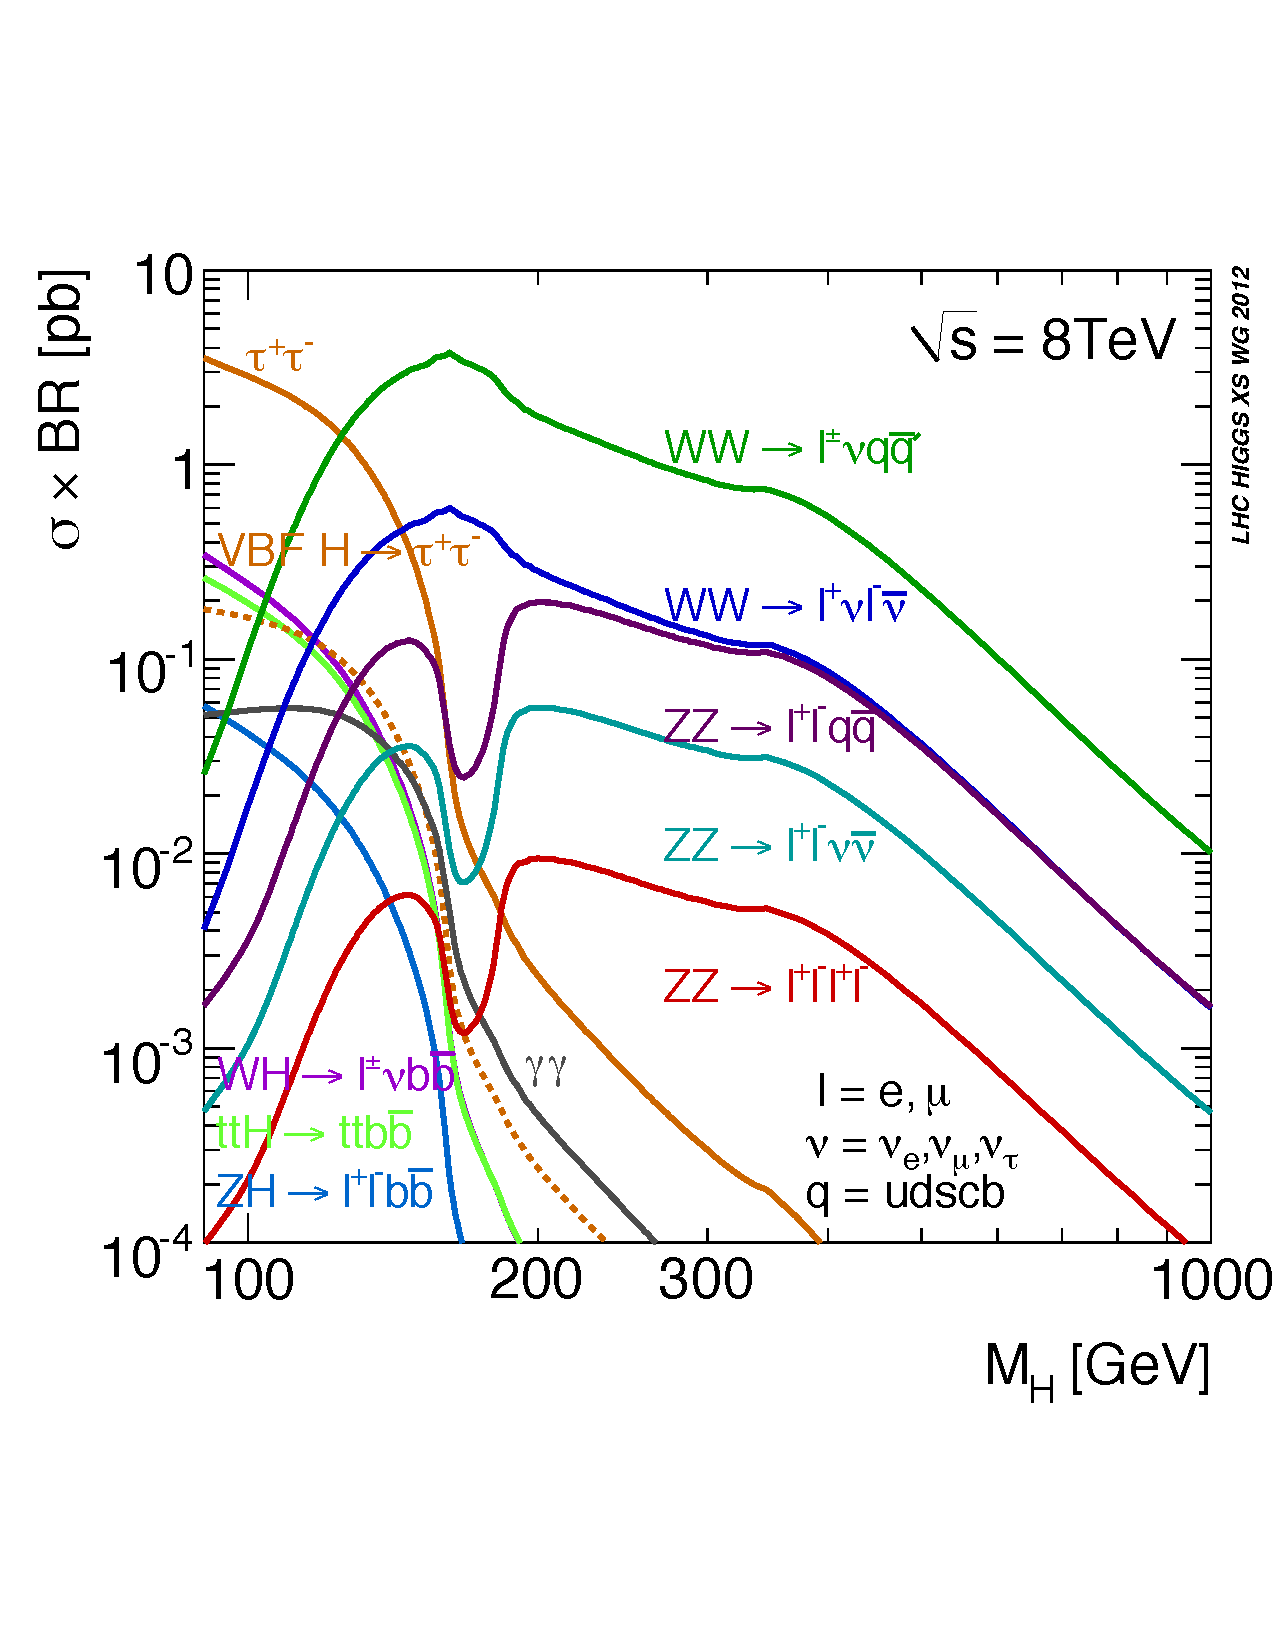
\includegraphics[width=0.46\linewidth]{{LHC_Pheno/XSBR_8TeV_SM_HM}.pdf}
\caption[(left) Standard Model Higgs boson decay branching ratios for selected decay modes, of specific interest for this thesis is the $ZZ$ branching ratio. (right) Branching ratio times cross section for selected final states, of specific interest for this thesis is the $ZZ \to 4\ell\left(\ell^{+}\ell^{-}\ell^{+}\ell^{-}\right)$.]{(left) Standard Model Higgs boson decay branching ratios for selected decay modes, of specific interest for this thesis is the $ZZ$ branching ratio. (right) Branching ratio times cross section for selected final states, of specific interest for this thesis is the $ZZ \to 4\ell\left(\ell^{+}\ell^{-}\ell^{+}\ell^{-}\right)$\cite{Dittmaier:2012vm, Heinemeyer:2013tqa}.}
\label{fig:Higgs_BR}
\end{center}
\end{figure}

Of specific interest for this thesis is the Higgs boson decay to the $ZZ \to 4\ell$ final state, shown in figure \ref{fig:H_ZZ_4l_Feyn}. Where we consider $\ell = e, \mu$ because these leptons will be long lived enough to be detected directly by CMS, making them distinct from $\tau$ leptons which often decay because of their high mass. The $ZZ$ branching ratio is one of the highest across a wide rage of possible Higgs boson masses, making it advantageous for search and characterization studies. The $4\ell$ final state is used not because it has a particularly high cross section times branching ratio (seen in figure \ref{fig:Higgs_BR} right), but because there are low SM background contributions and because all of the final particles are directly detected by the CMS detector.

\begin{figure}
\begin{center}
\unitlength=2mm
\begin{fmffile}{H_ZZ_4l_Feyn}
\begin{fmfgraph*}(40,30) 
  \fmfleft{i1} \fmfright{sp1,sp2,sp3,sp4}
  \fmf{dashes,label=$H$}{i1,v1} 
  \fmf{boson,label=$Z$}{v1,v2}
  \fmf{boson,label=$Z$}{v1,v3}
  \fmf{fermion,label=$e/\mu$}{sp1,v2,sp2}
  \fmf{fermion,label=$e/\mu$}{sp3,v3,sp4}
\end{fmfgraph*}

\end{fmffile}
\end{center}
\caption[Feynman diagram depicting Higgs boson decay into two Z bosons and subsequently into four leptons $H \to ZZ \to 4\ell$.]{Feynman diagram depicting Higgs boson decay into two Z bosons and subsequently into four leptons $H \to ZZ \to 4\ell$.}
\label{fig:H_ZZ_4l_Feyn}
\end{figure}

This thesis considers all of the data collected by CMS during run 1 of the LHC proton-proton collisions. This corresponds to an integrated luminosity of $\unit{5.1}{\invfemtobarn}$ collected at a center of mass energy of $\sqrt{s} = \unit{7}{\TeV}$ and $\unit{19.7}{\invfemtobarn}$ collected at $\sqrt{s} = \unit{8}{\TeV}$. The search for and later characterization of a Higgs boson requires that there be two pairs of same-flavor, opposite-charge, well-identified isolated leptons $\left(e^{+}e^{-}e^{+}e^{-}, \mu^{+}\mu^{-}\mu^{+}\mu^{-}, \text{ or } e^{+}e^{-}\mu^{+}\mu^{-}\right)$ compatible with an intermediate state of $ZZ$. Computability with $ZZ$ is defined such that one or both of the $Z$'s can be off the mass resonance of the Z-boson.

In this case, a Higgs boson signal will appear as a narrow mass peak on top of a smooth background when observing the four lepton mass distribution. The search is conducted in a mass range of $m_{4\ell} \in \unit{110 -- 1000}{\GeV}$. For low-mass Higgs bosons $\left(m_{H} < \unit{400}{\GeV}\right)$, the width of the resonance in $m_{4\ell}$ is very well peaked and described with a Breit-Wigner distribution. For higher mass Higgs bosons $\left(m_{H} > \unit{400}{\GeV}\right)$, the width of the $m_{4\ell}$ mass peak is much broader and described in the complex pole scheme \cite{Dittmaier:2011ti, Dittmaier:2012vm, Heinemeyer:2013tqa}. Detailed analysis of the width of the Higgs boson will be discussed in section \ref{sec:Higgs_Width_Pheno}.

\begin{figure}
\begin{center}
\unitlength=2mm
\begin{fmffile}{qq_ZZ_4l_Feyn}
\begin{fmfgraph*}(40,15) 
  \fmfleft{i1,i2} \fmfright{sp1,sp2,sp3,sp4}
  \fmf{fermion,label=$q$}{i1,v1,v2,i2} 
  \fmffixed{(.3w,0)}{i1,v1}
  \fmffixed{(.3w,0)}{i2,v2}
  %\fmffixed{(0,.3h)}{v2,v1}
  \fmf{boson,label=$Z$}{v1,v3}
  \fmf{boson,label=$Z$}{v2,v4}
  \fmffixed{(.3w,0)}{v1,v3}
  \fmffixed{(.3w,0)}{v2,v4}
  %\fmf{fermion,label=$e/\mu$}{sp1,v3,sp2}
  %\fmf{fermion,label=$e/\mu$}{sp3,v4,sp4}
\end{fmfgraph*}

\end{fmffile}
\end{center}
\caption[Feynman diagram depicting the quark production of two Z bosons $qq \to ZZ$.]{Feynman diagram depicting the quark production of two Z bosons $qq \to ZZ$.}
\label{fig:qq_ZZ_4l_Feyn}
\end{figure}

\begin{figure}
\begin{center}
\unitlength=2mm
\begin{fmffile}{gg_ZZ_4l_Feyn}
\begin{fmfgraph*}(40,15) 
  \fmfleft{i1,i2} \fmfright{sp1,sp2,sp3,sp4}
  \fmf{gluon,label=$g$}{i1,v1} 
  \fmf{gluon,label=$g$}{i2,v2} 
  \fmffixed{(.3w,0)}{i1,v1}
  \fmffixed{(.3w,0)}{i2,v2}
  \fmf{fermion,label=$q$}{v1,v2,v3,v4,v1}
  \fmffixed{(.3w,0)}{v2,v3}
  \fmffixed{(.3w,0)}{v1,v4}
  \fmf{boson,label=$Z$}{v3,v5}
  \fmf{boson,label=$Z$}{v4,v6}
  \fmffixed{(.3w,0)}{v3,v5}
  \fmffixed{(.3w,0)}{v4,v6}
  %\fmf{fermion,label=$e/\mu$}{sp1,v6,sp2}
  %\fmf{fermion,label=$e/\mu$}{sp3,v5,sp4}
\end{fmfgraph*}

\end{fmffile}
\end{center}
\caption[Feynman diagram depicting the gluon production of two Z bosons $gg \to ZZ$.]{Feynman diagram depicting the gluon production of two Z bosons $gg \to ZZ$.}
\label{fig:gg_ZZ_4l_Feyn}
\end{figure}

The background in the $4\ell$ final state is dominated by the SM $q\bar{q} \to ZZ \to 4\ell$ production, shown in figure \ref{fig:qq_ZZ_4l_Feyn}. This background is not particularly large but it cannot be reduced with quality cuts on the leptons or tuning of phase space without significant losses to the expected signal. Additionally, there will be SM $gg \to ZZ \to 4\ell$, shown in figure \ref{fig:gg_ZZ_4l_Feyn}. Z boson production from gluons is also irreducible, but this contribution is about 10\% of the dominant $qq \to ZZ \to 4\ell$ production. As discussed in the next section, this $gg \to ZZ$ contribution can actually be exploited to study the properties of any new resonance. There will also be background contributions from collisions that produce a Z boson in addition to other jets or particles that are mis-identified as leptons. This background is reducible by tuning the analysis to remove as much of this noise as possible. This tuning is done by adjusting the quality requirements on the leptons and requirements about where the events fall in phase space. This process is described more in section \ref{sec:BkgEstimation}.

\section{Higgs boson width: off resonance production and decay}
\label{sec:Higgs_Width_Pheno}

When a new particle is observed, one of the fundamental properties that we would like to understand is the width of the mass resonance. From Einstein's mass--energy equivalence we know that the mass of a particle is equal to the amount of energy it has (in natural units). So by measuring the width of a resonance's mass spectrum $\left(\Gamma\right)$ we have a measure of the natural spread in energies that the particle can take. For this discussion we will operate under the assumption that the Higgs boson mass $m_{H} \sim \unit{125 -- 126}{\GeV}$. In later sections, will we present the results of the Higgs boson search upon which these were made.

Armed with this measurement of the natural energy spread of a particle, one can deduce the mean lifetime $\left(\tau\right)$ of the particle. The lifetime and a particles energy are related by the time--energy formulation of the Heisenberg uncertainty principle. Simply, this states that $\Delta E \Delta t \geq 1/2$. So measuring the spread in energies for an unstable particle one can deduce the lifetime by the simple relation $\Gamma/2 = 1/2\cdot 1/\tau$. 

This width can also illuminate possible new physics. The lifetime of a particle is determined by the rate that it decays into other particles. This rate is determined by the number of possible states it can decay into. So a particle that can only decay into a small number of particles will have a longer lifetime. The lifetime of the Higgs boson will be determined by its rate of decay into SM particles and particles not yet described by the SM. So gaining an accurate measurement of the Higgs boson lifetime can be a key into new possible particles that it couples to. The predicted width for a Higgs boson decaying only to SM particles is given in figure \ref{fig:Higgs_width}, if you compare this width to the plot of the branching rations in figure \ref{fig:Higgs_BR} (left) you will see that when new decay modes become available the width increases.

\begin{figure}
\begin{center}
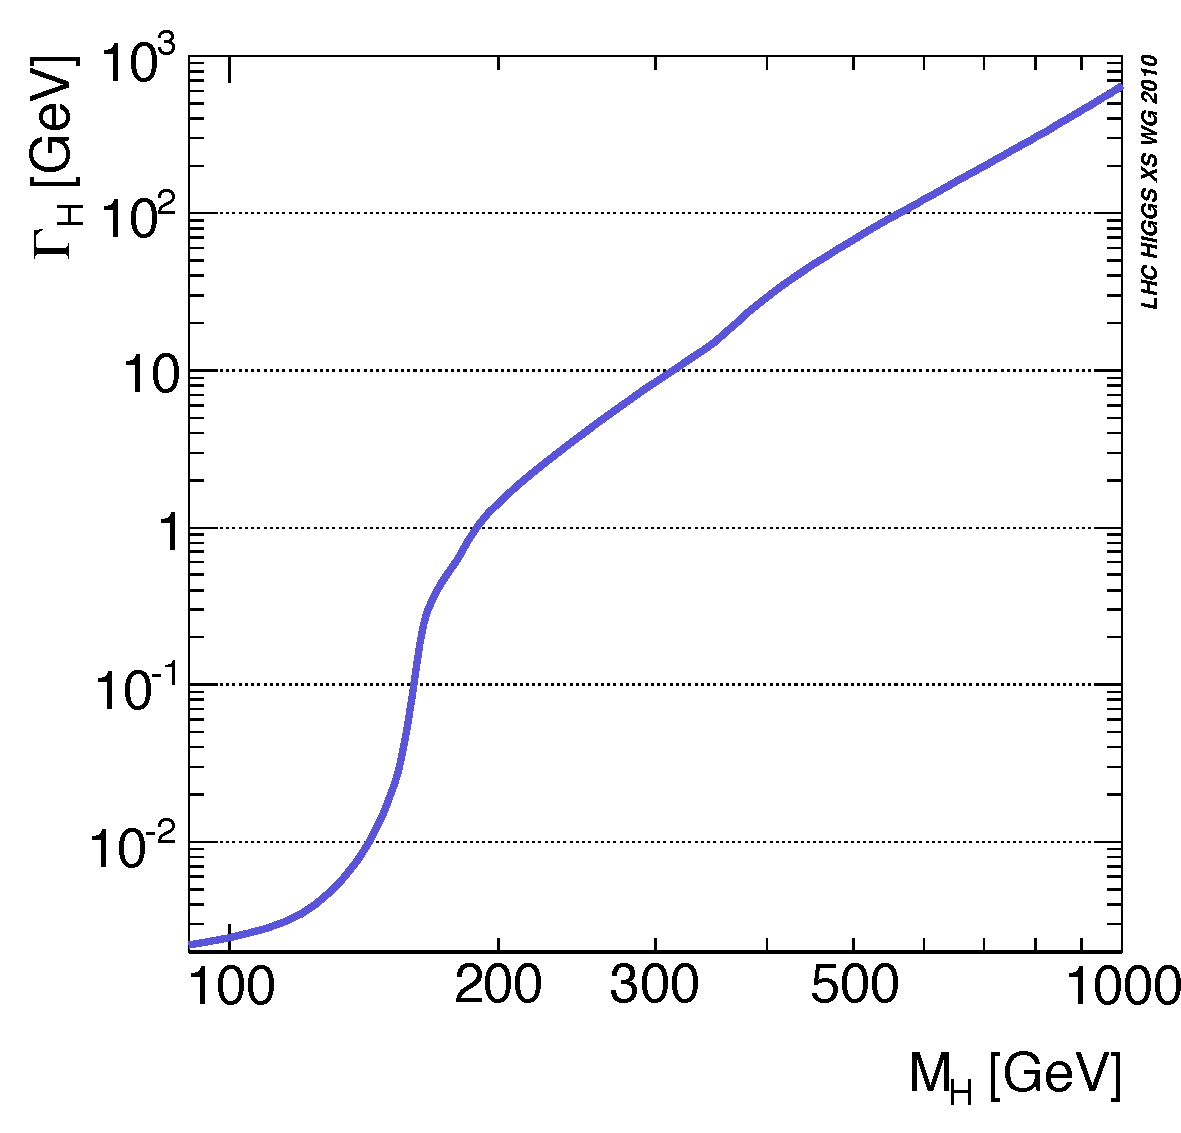
\includegraphics[width=0.46\linewidth]{{LHC_Pheno/YRHXS_BR_fig2}.pdf}
\caption[Total width of the SM Higgs boson as a function of its mass.]{Total width of the SM Higgs boson as a function of its mass\cite{Dittmaier:2011ti}.}
\label{fig:Higgs_width}
\end{center}
\end{figure}

As described in section \ref{sec:TriggerANDreconstruction}, CMS has a very fine momentum resolution for both electrons and muons. This allows CMS to accurately measure the mass and width of any new observed resonance very well, on the order of $\sim\unit{\text{few}}{\GeV}$. However, as shown in figure \ref{fig:Higgs_width} for low mass Higgs bosons the width can be quite small, on the order of $\sim\MeV$. Thus, direct measurement of the natural width of a low-mass Higgs boson will be dominated by the experimental resolution.

To overcome this, recent theoretical work has illuminated a way to measure the total width of a low-mass Higgs boson without looking at the width of the mass resonance directly. This technique relies on the ratio of the on resonance and off resonance production of the new boson. When the new boson is observed on resonance, the mass will be $m_{H} \sim \unit{125 -- 126}{\GeV}$, because this mass $m_{H} < 2m_{Z} = 2\left(\unit{91.2}{\GeV}\right)$ the Higgs boson will be real and will decay into one or more virtual Z bosons. Virtual particles are particles who's mass is not at the natural resonance, usually denoted $Z^{*}$, while real particles which have a mass at the natural resonance. For the dominant production mechanism, we have $gg \to H \to Z^{\left(*\right)}Z^{*} \to 4\ell$.

\begin{figure}
\begin{center}
\unitlength=1mm
\begin{fmffile}{ggH_ZZ_Feyn}

\begin{fmfgraph*}(40,20) 
  \fmfleft{i1,i2} \fmfright{sp1,sp2}
  \fmf{gluon,label=$g$}{i1,v1} 
  \fmf{gluon,label=$g$}{i2,v2}
  \fmf{fermion}{v1,v2,v3,v1}
  \fmffixed{(0,.5h)}{v1,v2}
  \fmf{dashes,label=$H$}{v3,v4}
  \fmffixed{(.3w,0)}{v3,v4}
  \fmf{boson,label=$Z$}{v4,sp1}
  \fmf{boson,label=$Z$}{v4,sp2}
\end{fmfgraph*}
\begin{fmfgraph*}(40,20) 
  \fmfleft{i1,i2} \fmfright{sp1,sp2,sp3,sp4}
  \fmf{gluon,label=$g$}{i1,v1} 
  \fmf{gluon,label=$g$}{i2,v2} 
  \fmffixed{(.5w,0)}{i1,v1}
  \fmffixed{(.5w,0)}{i2,v2}
  \fmf{fermion,label=$q$}{v1,v2,v3,v4,v1}
  \fmffixed{(.5w,0)}{v2,v3}
  \fmffixed{(.5w,0)}{v1,v4}
  \fmf{boson,label=$Z$}{v3,v5}
  \fmf{boson,label=$Z$}{v4,v6}
  \fmffixed{(.3w,0)}{v3,v5}
  \fmffixed{(.3w,0)}{v4,v6}
\end{fmfgraph*}

\end{fmffile}
\end{center}
\caption[(top) Feynman diagram depicting Higgs boson production through gluon-gluon fusion and subsequent decay to two Z bosons $gg \to H \to ZZ$. (bottom) Feynman diagram depicting ZZ production through gluon-gluon fusion $gg \to ZZ$. These two diagrams will interfere with eachother having an affect on the final number of events observed in the $4\ell$ final state.]{(top) Feynman diagram depicting Higgs boson production through gluon-gluon fusion and subsequent decay to two Z bosons $gg \to H \to ZZ$. (bottom) Feynman diagram depicting ZZ production through gluon-gluon fusion $gg \to ZZ$. These two diagrams will interfere with each other having an affect on the final number of events observed in the $4\ell$ final state.}
\label{fig:gg_??_ZZ_Feyn}
\end{figure}

However, the LHC will produce Higgs bosons far from this mass resonance as well. In this case, the Higgs boson will be virtual while the two Z bosons will both be  real, $gg \to H^{*} \to ZZ \to 4\ell$. In reference \cite{Kauer:2012hd} the authors point out that $\sim 10\%$ of the total Higgs boson cross section will produce Higgs bosons with a mass $m_{4\ell} > 2m_{Z}$. A plot of the Higgs boson mass shape is from this reference is shown in figure \ref{fig:Higgs_lineshape} for the ZZ and the WW final states. From this plot one can see the large fraction of the cross section that appears in this high mass window.

\begin{figure}
\begin{center}
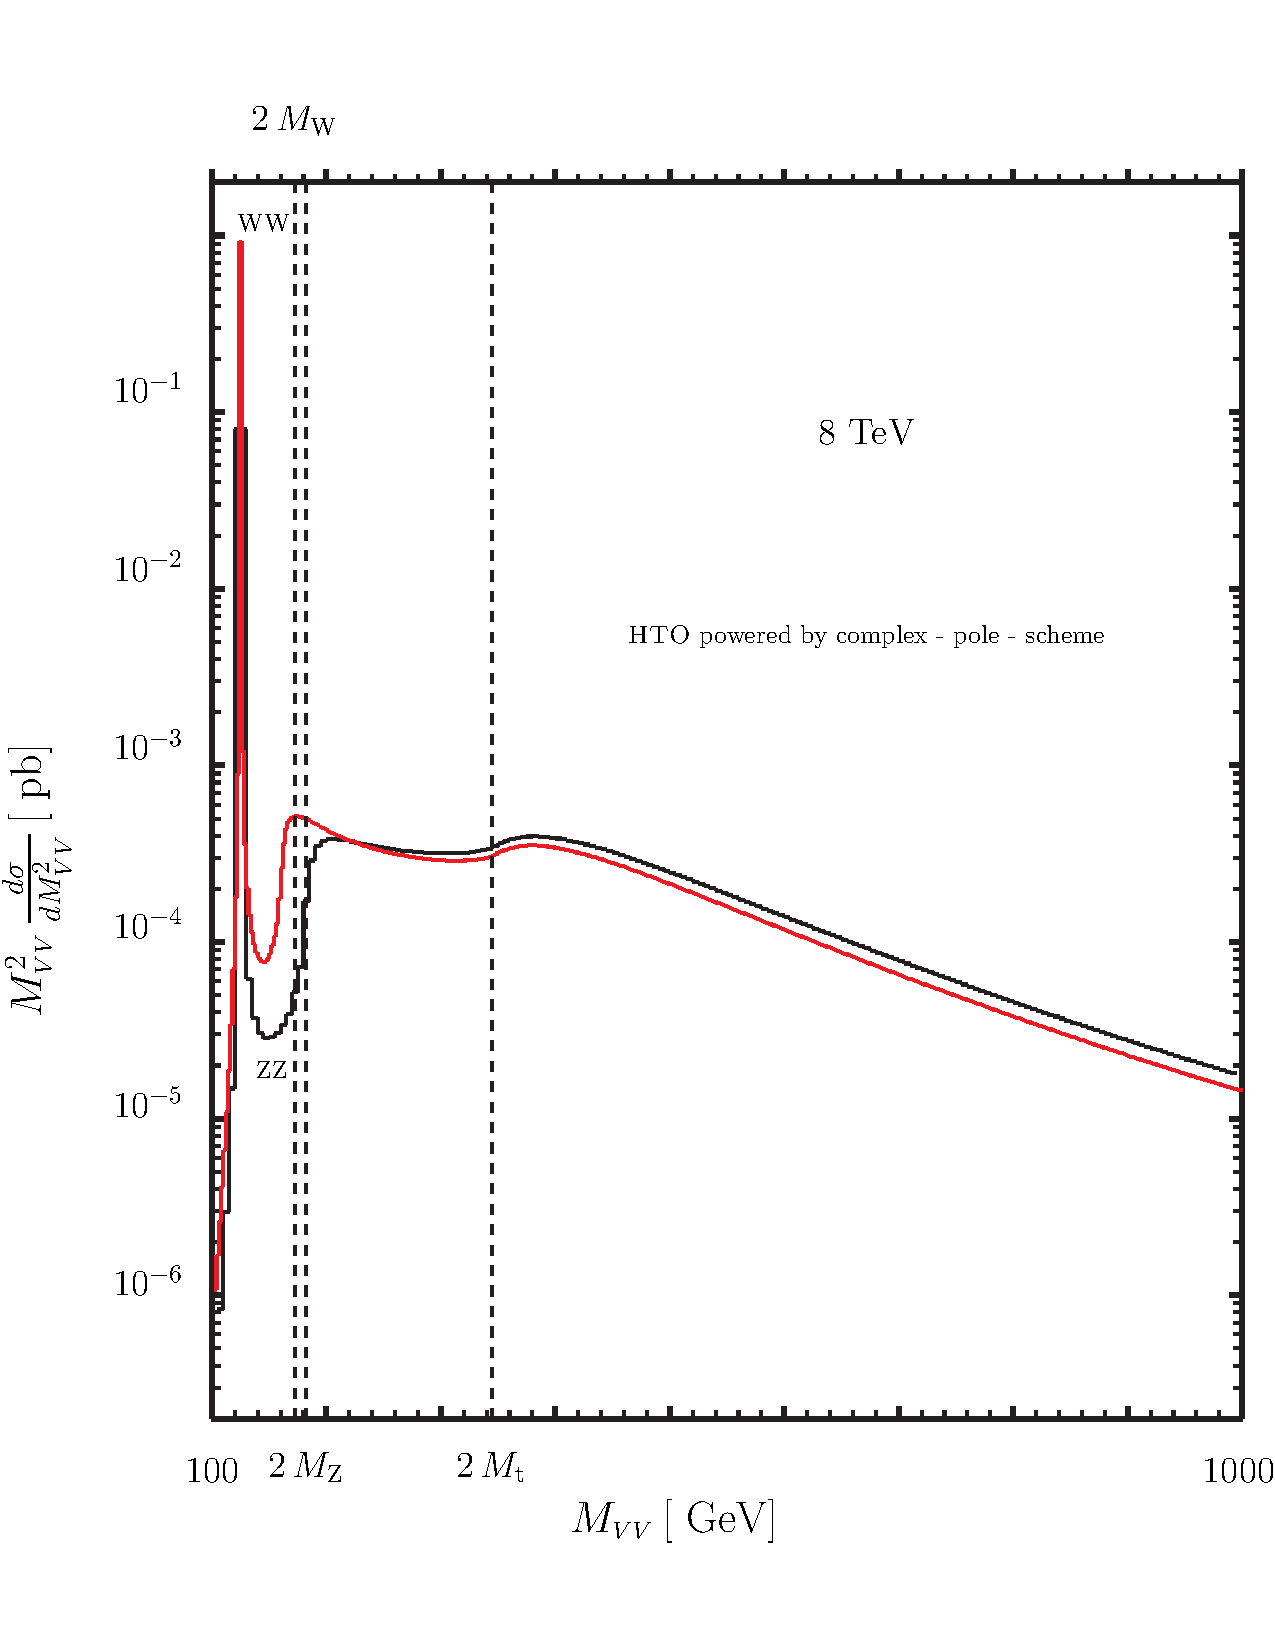
\includegraphics[width=0.46\linewidth]{{LHC_Pheno/lhzwa_fig1b}.pdf}
\caption[The NNLO ZZ (black) and WW (red) invariant mass distributions for $m_{H} = \unit{125}{\GeV}$.]{The NNLO ZZ (black) and WW (red) invariant mass distributions for $m_{H} = \unit{125}{\GeV}$\cite{Kauer:2012hd}.}
\label{fig:Higgs_lineshape}
\end{center}
\end{figure}

Following \cite{Caola:2013yja}, we can investigate the total width of the Higgs boson by comparing the on resonance and off resonance cross sections. Generally, the differential cross section of a Higgs boson produced through gluon-gluon fusion decaying into two Z bosons is given by equation \eqref{eq:diff_xsec}. Where $g_{ggH}$ is the effective coupling of the Higgs boson to gluons, $g_{HZZ}$ is the coupling of the Higgs boson to Z bosons, and $\Gamma_{H}$ is the total width of the Higgs boson. Also notice the demarcation of the observed mass of the $4\ell$ system, $m_{4\ell}$, is not necessarily the same as the Higgs boson mass $m_{H}$.

\begin{equation}
\label{eq:diff_xsec}
\frac{d\sigma_{gg \to H \to ZZ}}{d m_{4\ell}} \sim \frac{g_{ggH}^{2}g_{HZZ}^{2}}{\left(m_{4\ell}^{2} - m_{H}^{2}\right)^{2} + m_{H}^{2}\Gamma_{H}^2} 
\end{equation}

When a Higgs boson is produced on the resonance peak $m_{4\ell} \sim m_{H}$ then the mass integral can be evaluated assuming the second term in the denominator will be larger than the first. Giving the on peak cross section in equation \eqref{eq:onpeak_xsec} note that the cross section is proportional to the couplings and inversely the total width of the Higgs boson. However, if a Higgs boson is produced off of the resonance peak, specifically when $m_{4\ell} - m_{H} \gg \Gamma_{H}$, then the cross section becomes independent of the width. Shown in equation \eqref{eq:offpeak_xsec} the off peak cross section becomes proportional to the couplings but the width does not contribute.

\begin{equation}
\label{eq:onpeak_xsec}
\sigma_{gg \to H \to ZZ}^{\text{on peak}} \sim \frac{g_{ggH}^{2}g_{HZZ}^{2}}{\Gamma_{H}} 
\end{equation}

\begin{equation}
\label{eq:offpeak_xsec}
\sigma_{gg \to H \to ZZ}^{\text{off peak}} \sim g_{ggH}^{2}g_{HZZ}^{2} \sim \sigma_{gg \to H \to ZZ}^{\text{on peak}} \times \Gamma_{H}
\end{equation}

From these results we can see that the number of events that are produced on the mass resonance peak is dependent upon the total width of the new boson, while the number of events produced off peak are only dependent upon the couplings to the other SM particles. Thus, as pointed by \cite{Caola:2013yja} measuring the ratio of the on peak and off peak Higgs boson production is equivalent to measuring the total width of the new boson.

Complicating this story, is the quantum mechanical interference between the different $gg \to \ldots \to 4\ell$ processes. While this interference is present for the entire $m_{4\ell}$ range considered in this thesis, at low masses it is a very small and negligible. Above the $2m_{Z}$ mass, the interference between $gg \to ZZ \to 4\ell$ and $gg \to H^{*} \to ZZ \to 4\ell$, figure \ref{fig:gg_??_ZZ_Feyn}, processes needs to be considered. While the off peak signal contribution will scale by $\sigma_{gg \to H \to ZZ}^{\text{on peak}} \times \Gamma_{H}$ the interference between the signal and background term will scale by $\sqrt{\sigma_{gg \to H \to ZZ}^{\text{on peak}} \times \Gamma_{H}}$. 

The impact of these three terms is seen in figure \ref{fig:Higgs_sig/bkg/interf}. Here, one can clearly see the large difference between ignoring (cyan) and correctly accounting (black) for the interference in this region. Neglecting interference one would anticipate a large increase in the yield of the high mass $gg \to \ldots \to ZZ$ contribution, but since the interference between off resonance Higgs boson production and the $gg \to ZZ$ continuum background is destructive, the SM actually predicts that the high mass contribution will be lower than otherwise anticipated.

\begin{figure}
\begin{center}
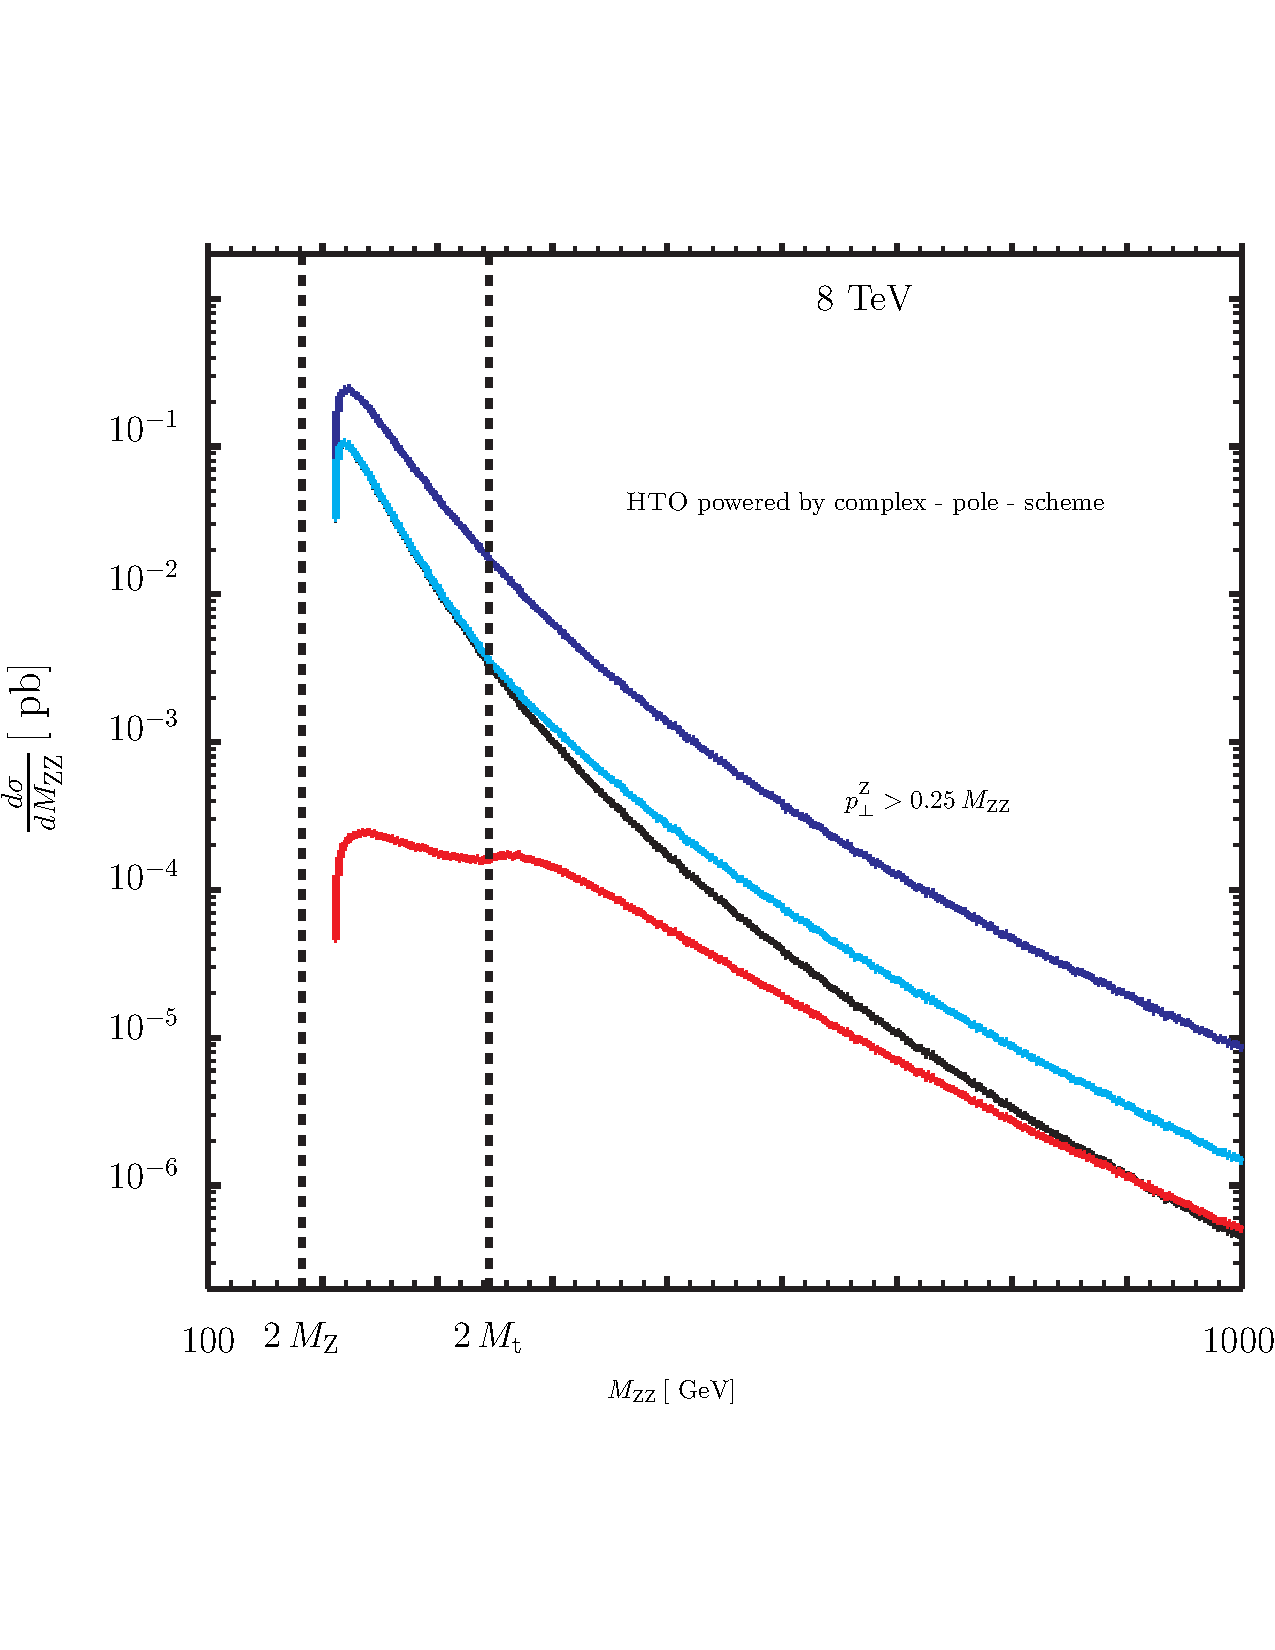
\includegraphics[width=0.46\linewidth]{{LHC_Pheno/lhzwa_fig2}.pdf}
\caption[The LO $ZZ$ invariant mass distribution $gg \to ZZ$ for $m_{H} = \unit{125}{\GeV}$. Black is the total $gg \to \ldots \to ZZ$ contribution once all interfrence effects are taken into account. Red is the $gg \to H^{*} \to ZZ$ signal only, and cyan is the $gg \to \ldots \to ZZ$ contribution ignoring the interference between the two contributions. For scale, the $q\bar{q} \to ZZ$ contribution is shown in blue.]{The LO $ZZ$ invariant mass distribution $gg \to ZZ$ for $m_{H} = \unit{125}{\GeV}$. Black is the total $gg \to \ldots \to ZZ$ contribution once all interfrence effects are taken into account. Red is the $gg \to H^{*} \to ZZ$ signal only, and cyan is the $gg \to \ldots \to ZZ$ contribution ignoring the interference between the two contributions. For scale, the $q\bar{q} \to ZZ$ contribution is shown in blue \cite{Kauer:2012hd}.}
\label{fig:Higgs_sig/bkg/interf}
\end{center}
\end{figure}

\begin{figure}
\begin{center}
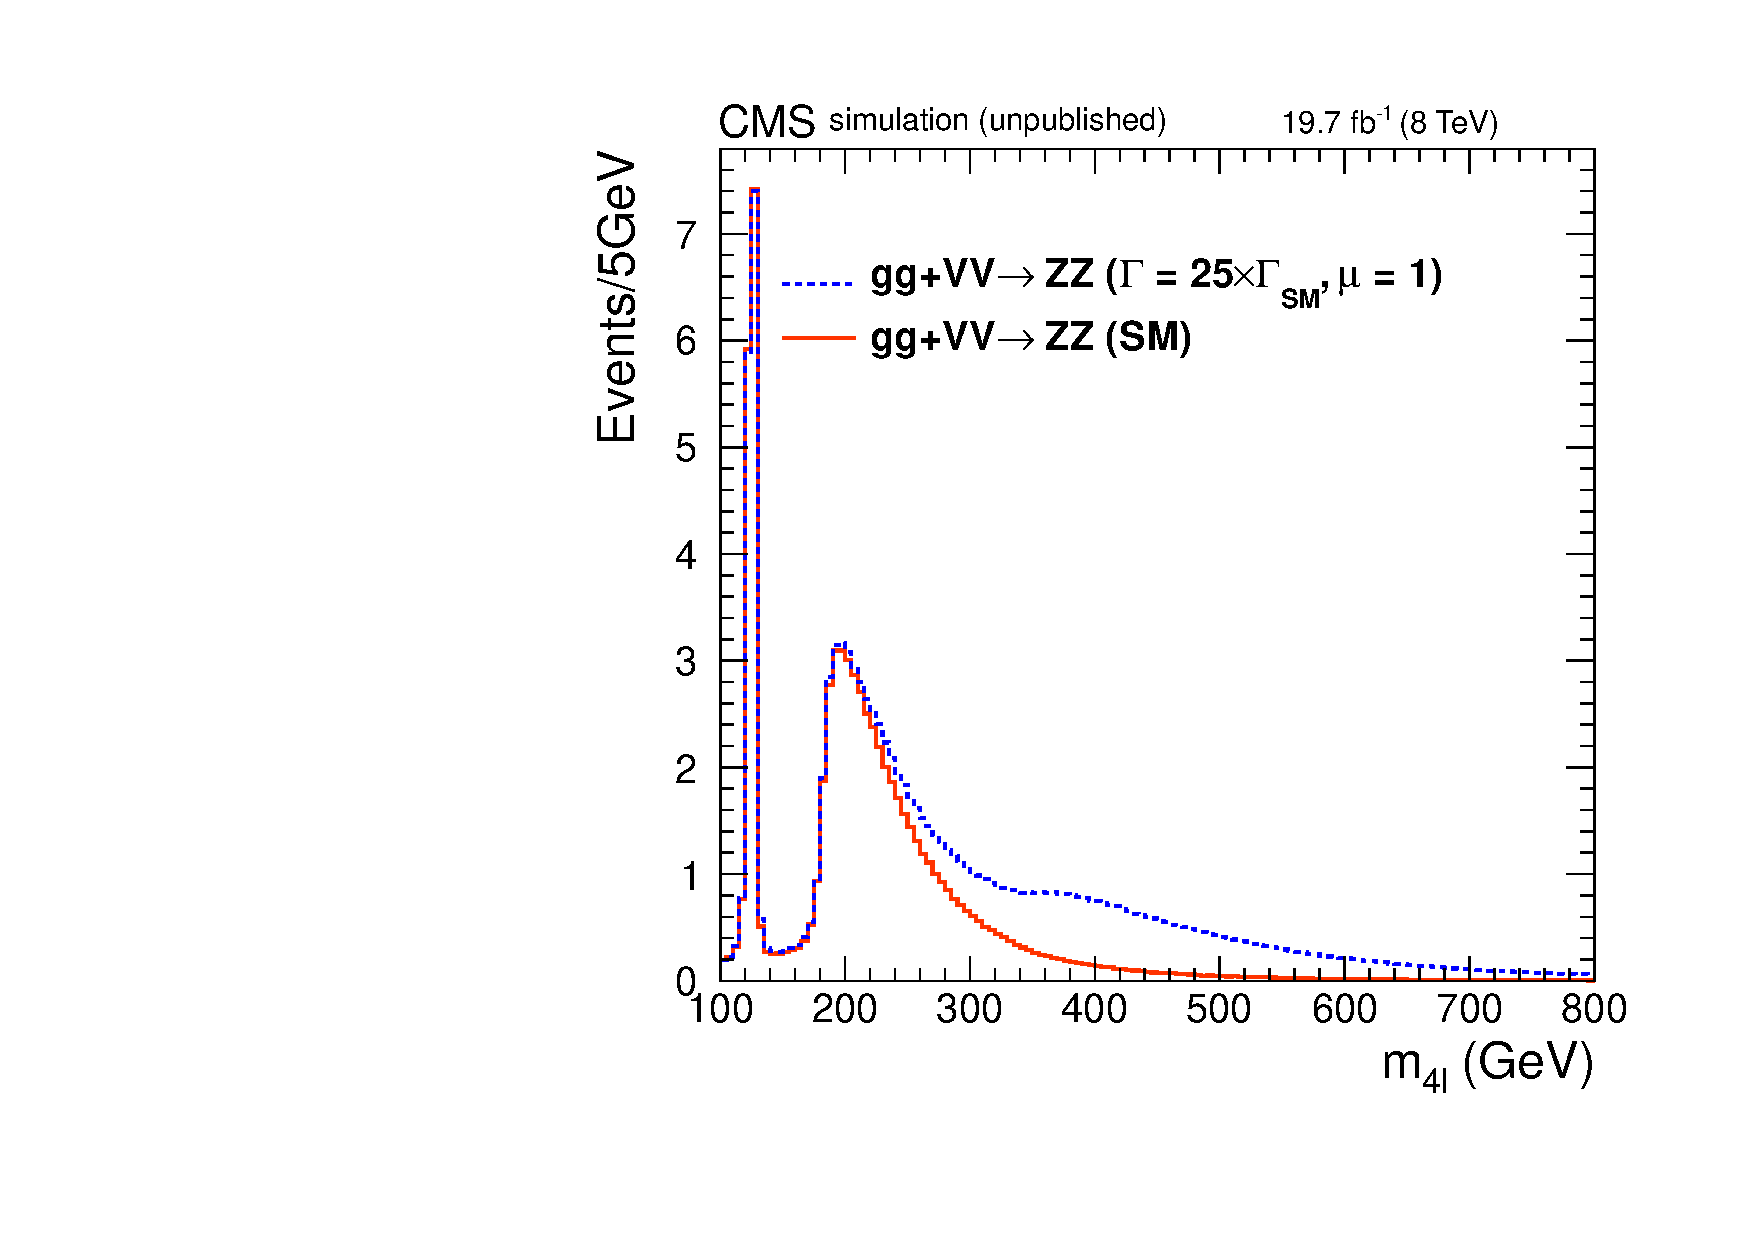
\includegraphics[width=0.46\linewidth]{{LHC_Pheno/ZZMass_100-800_SIM_20May2014}.pdf}
\caption[Distribution of the expected four-lepton reconstructed mass in full analysis mass range for the sum of the $4e$, $4\mu$, and $2e2\mu$ channels and for $gg+VV \to ZZ$ processes for a Higgs boson mass of $\unit{125.6}{\GeV}$. The expected distribution for a scenario corresponding to a scaling of the width by 25 is also shown. This illustrates the expected change in $gg+VV \to ZZ$ production when changing the Higgs boson width and at the same time constraining the peak cross section to the SM expectation.]{Distribution of the expected four-lepton reconstructed mass in full analysis mass range for the sum of the $4e$, $4\mu$, and $2e2\mu$ channels and for $gg+VV \to ZZ$ processes for a Higgs boson mass of $\unit{125.6}{\GeV}$. The expected distribution for a scenario corresponding to a scaling of the width by 25 is also shown. This illustrates the expected change in $gg+VV \to ZZ$ production when changing the Higgs boson width and at the same time constraining the peak cross section to the SM expectation \cite{Khachatryan:2014iha}.}
\label{fig:CMS_gg_ZZ}
\end{center}
\end{figure}

The resulting $m_{4\ell}$ distributions for two hypothetical bosons are shown in figure \ref{fig:CMS_gg_ZZ}, they both have the same on peak cross section but different total widths. The result is a change in the total number of events expected in the analysis. Additionally, the shape of the $m_{4\ell}$ distribution and the kinematics of the $4\ell$ will be different. A detailed description of how all of these factors are used to determine the width is given in section \ref{sec:Width_Experiment}. Also included in this image and analysis is the analogous effect for the VBF production mode.

\section{Spin and Parity of a Single-Produced Resonance}
\label{sec:Higgs_Spin_Pheno}

Using the decay rates and kinematics of a newly observed resonance one can piece together the quantum mechanical properties of the original boson. Once a new particle is observed, its spin and parity quantum numbers need to be determined. This will confirm if the new particle is the Higgs boson that was predicted or something entirely, or partially, different. Using the $H \to ZZ \to 4\ell$ decay channel is the best way to study these properties because of the small, well understood background contributions, and because all of the final state particles can be detected by CMS and have excellent precision. 

In basic terms, when a new particle is produced in a collision its spin and parity quantum numbers restrict the allowed types of interactions it can have with SM particles. This feature can be observed by investigating the kinematic distributions of the decay products or the particles produced in association with the new resonance. Of particular interest for this thesis work are the $X \to VV$ couplings (HVV). Where $V$ is any vector boson (Z, W, $\gamma$, g), and $X$ is the new resonance. When this new resonance is spin-0, we will use $H$ because the Higgs boson is predicted to be spin-0. While this vertex can be studied by using the production or decay of a new particle we will focus on the properties that can be determined from the decay products. 

When a new boson is produced it can be either spin-zero, one, or two\footnote{Unless, the resonance is actually two particles with a mass difference less than the experimental resolution.}. In this work each is considered as a possibility for a new resonance, and the differences between their kinematics are used to study and classify the newly observed boson. The relevant phenomenology for these interactions is presented below.

\subsection{Decay of a spin-zero resonance}
\label{sec:Spin0_Pheno}

The scattering amplitude describing the interaction between a spin-zero H boson and two spin-one gauge bosons $VV$ $\left(ZZ, Z\gamma, \gamma\gamma, WW \text{ or } gg\right)$ can be defined as in equation \eqref{eq:formfact-fullampl-spin0}. Where the coupling parameters $a_{i}^{VV}$ can have both real and imaginary parts and in general are form factors which can depend on the suared Lorentz invariant four-momenta of $V_{1}$ and $V_{2}$, $q_{V1}^2$ and $q_{V2}^2$. In this expression, terms of higher order than $q_{V}^2$ have been dropped in the expansion under the assumption that anomalous couplings will only have a small contribution. In this expression, we use a different notation than previous sections and label the field strength tensor of a gauge boson with momentum $q_{Vi}$ and polaraization $\epsilon_{Vi}$ with $f^{\left(i\right) \mu \nu} = \epsilon^{\mu}_{Vi}q_{Vi}^{\nu} - \epsilon^{\nu}_{Vi}q_{Vi}^{\mu}$. ${\tilde f}^{\left(i\right)}_{\mu \nu} = \frac{1}{2}\epsilon_{\mu\nu\rho\sigma}f^{\left(i\right) \rho \sigma}$ is the dual field strength tensor, and the superscript $*$ designates a complex conjugate. The masses of the Z or W boson is labeled as $m_{V1}$, while in the case of massless bosons there is no contribution from this term. To understand the impact form factor will have on the $a_{1}$ term, an energy scale $\Lambda_{1}$ for beyond-SM physics that could impact the SM scattering amplitude is also studied \cite{Anderson:2013afp}. 

\begingroup
\small
\begin{equation}
A(H\to VV) \sim
\left[ a_{1}^{VV}
+ \frac{\kappa_1^{VV}q_{V1}^2 + \kappa_2^{VV} q_{V2}^{2}}{\left(\Lambda_{1}^{VV} \right)^{2}} \right]
m_{V1}^2 \epsilon_{V1}^* \epsilon_{V2}^*
+ a_{2}^{VV}  f_{\mu \nu}^{*(1)}f^{*(2)\mu\nu}
+ a_{3}^{VV}   f^{*(1)}_{\mu \nu} {\tilde f}^{*(2)\mu\nu}
\label{eq:formfact-fullampl-spin0}
\end{equation}
\endgroup

In the SM, the tree-level contribution from $ZZ \left(WW\right)$ correspond to $a_{1}^{ZZ \left(WW\right)} \neq 0$, while the loop-induced SM contribution for $Z\gamma, \gamma\gamma, \text{ and } gg$ is $a_{2}^{VV} \neq 0$. Small SM contributions to the higher order $a_{i}$ terms can come from loop level contributions but, in general, these should be small. Additional restrictions on the allowed values for the $\kappa_{i}$ terms arise from symmetry and gauge invariance. For $ZZ$, they require $\kappa_{1}^{ZZ} = \kappa_{2}^{ZZ} = - \text{exp}\left(-i\phi_{\Lambda1}^{ZZ}\right)$ where $\phi_{\Lambda1}^{ZZ}$ is the relative phase between the $a_{1}^{ZZ}$ and $\Lambda_{1}$ terms. 

The parity conserving contribution from a pseudoscalar particle $\left( 0^{+-}, CP\text{-odd} \right)$ would be generated by the $a_{3}$ term, while a higher order scalar $\left( 0^{++}, CP\text{-even} \right)$ would be generated by $a_{2}$ or $\Lambda_{1}$ contributions. Anomalous contributions for the $\Lambda_{1}, a_{2}, \text{ or } a_{3}$ terms could be a sign of BSM physics and can in general have be complex, allowing for a relative phase between them and the SM $a_{1}$ term. To determine if these anomalous terms contribute to an observed resonance, we parameterize the contribution of one of these terms in an effective cross section fraction. These fractions are given in equation \eqref{eq:fa_definitions}, where $\sigma_{i}$ is the cross section for an $a_{i} = 1, a_{j\neq i} = 0$ particle decaying to the $2e2\mu$ final state\footnote{$\tilde{\sigma}_{\Lambda{1}}$ is the effective cross section of the process corresponding to $\Lambda_{1} = \unit{1}{\TeV}$, given in units of $\femtobarn\cdot\TeV^{4}$.}. The phases $\phi_{ai}$ are used to generalize equation \eqref{eq:formfact-fullampl-spin0} so that the anomalous contributions to be complex.

\begin{eqnarray}
f_{\Lambda1} =& \frac{\tilde{\sigma}_{\Lambda1}/\left(\Lambda_{1}\right)^{4}}{\abs{a_1}^2 \sigma_{1} + \abs{a_2}^2 \sigma_{2} + \abs{a_3}^2 \sigma_{3} + \tilde{\sigma}_{\Lambda{1}}/\left(\Lambda_{1}\right)^{4} +\ldots}, &\phi_{\Lambda1}, \nonumber \\
f_{a2} =& \frac{\abs{a_2}^2 \sigma_{2}}{\abs{a_1}^2 \sigma_{1} + \abs{a_2}^2 \sigma_{2} + \abs{a_3}^2 \sigma_{3} + \tilde{\sigma}_{\Lambda{1}}/\left(\Lambda_{1}\right)^{4} +\ldots}, &\phi_{a2} = \text{arg}\left(\frac{a_{2}}{a_{1}}\right), \\
f_{a3} =& \frac{\abs{a_3}^2 \sigma_{3}}{\abs{a_1}^2 \sigma_{1} + \abs{a_2}^2 \sigma_{2} + \abs{a_3}^2 \sigma_{3} + \tilde{\sigma}_{\Lambda{1}}/\left(\Lambda_{1}\right)^{4} +\ldots}, &\phi_{a3} = \text{arg}\left(\frac{a_{3}}{a_{1}}\right), \nonumber
\label{eq:fa_definitions}
\end{eqnarray}


These fractions are especially useful because they allow for great flexibility in the measurements. They are independent of the collider energy so they can be used to compare measurements made at different facilities, they are independent of coupling notation so can be used to translate between many different formulations for the spin-0 interactions, and they are bounded between $0$ and $1$ which allows investigation of the full phase space. 

In CMS studies of these results, analogous fractions are created for the $WW, Z\gamma, \gamma\gamma$ final states. These fractions can be combined for $ZZ$ and $WW$ under different assumptions about the relationships between the $a_{i}^{VV}$ terms. These results were a direct consequence of these studies and are left as a reference for the reader \cite{Khachatryan:2014kca}. 

\subsection{Decay of a spin-one resonance}
\label{sec:Spin1_Pheno}

In the case of a spin-one resonance, the amplitude of its interaction with a pair of massive gauge bosons, ZZ or WW, consists of two independent terms, seen in equation \eqref{eq:ampl-spin1}.

\begin{equation}
A(X_{J=1} \to VV) \sim b_{1}^{VV}  \left[ \left(\epsilon_{V1}^{*}q\right)\left(\epsilon_{V2}^{*}\epsilon_{X}\right) + \left(\epsilon_{V2}^{*}q\right)\left(\epsilon_{V1}^{*}\epsilon_{X}\right) \right] + b_{2}^{VV}  \epsilon_{\alpha\mu\nu\beta}\epsilon_{X}^{\alpha}\epsilon_{V1}^{*\mu}\epsilon_{V2}^{*\nu}{\tilde q}^{\beta}
\label{eq:ampl-spin1}
\end{equation}

Where $\epsilon_{X}$ is the polarization vector of the boson $X$ with spin one, ${q}=q_{V1}+q_{V2}$ and ${\tilde q}=q_{V1}-q_{V2}$~\cite{Gao:2010qx, Bolognesi:2012mm}. Here the $b_{1}^{VV}  \neq 0$ coupling corresponds to a vector particle, while the $b_{2}^{VV} \neq 0$ coupling corresponds to a pseudovector. The $Z\gamma$ interactions of the spin-one particle are not considered, while the $\gamma\gamma$  and $gg$ interactions are forbidden by the Landau-Yang theorem~\cite{Landau:1948kw, Yang:1950rg}, where the $gg$ case is justified by the assumption that the state $X$ is color-neutral.

The evidence for a new boson in the $ZZ$ final state will be presented in section \ref{sec:Search_Results}, similar resonances have been seen in the $H \to \gamma\gamma$ decay channel, preventing the observation from being spin-one \cite{Aad:2012tfa,Chatrchyan:2012ufa,Chatrchyan:2013lba}. In the case that the $ZZ$ resonance is different than the one seen in these references, we test if an observed boson is more consistent with spin-one or the SM predicted Higgs boson. 

Pure vector $\left(1^{+}\right)$, pseudovector $\left(1^{-}\right)$, and mixed vector-pseudovector states are tested using the fraction $f_{b2}^{VV}$ given in equation \eqref{eq:fa_definitions_spin1}. This $f_{b2}^{VV}$ parameter is a continuous unique way to define any state that is a mixture of $1^{+}$ and $1^{-}$. Where $\sigma_{bi}$ is the cross section of the process corresponding to $b_{i} = 1, b_{j\neq i} = 0$ in the $X \to ZZ \to 2e2\mu$ final state.

\begin{equation}
f_{b2}^{VV}  = \frac{\abs{b_{2}^{VV}}^2 \sigma_{b2}}{\abs{b_{1}^{VV}}^2 \sigma_{b1} + \abs{b_{2}^{VV}}^2 \sigma_{b2}},
\label{eq:fa_definitions_spin1}
\end{equation}

\subsection{Decay of a spin-two resonance}
\label{sec:Spin2_Pheno}

In the case of a general spin-two resonance, we test if a new observation is more consistent with the SM Higgs boson or a spin-two boson. The amplitude to describe the $X \to ZZ$ production is given in equation \eqref{eq:ampl-spin2-a} (This same amplitude describes the $gg \to X$ production with $m_{V} = 0$.) where $t^{\mu\nu}$ is the wavefunction of a spin-two particle $X$ given by a symmetric traceless tensor, $m_{V}$ is the mass of the considered gauge boson, and $\Lambda$ is the scale of BSM physics~\cite{Gao:2010qx, Bolognesi:2012mm}. The couplings $c_{1}^{VV}$ and $c_{5}^{VV}$ correspond to the parity-conserving interaction of a spin-two tensor with minimal gravity-like couplings. As in the spin-zero case, the couplings $c_{i}^{VV}$ are in general momentum-dependent form factors. In this analysis it is assumed that the form factors are momentum-independent constants and, thus, only the lowest $q_i^2$  order terms in the scattering amplitude are considered \cite{Khachatryan:2014kca}.



\begin{multline}
\label{eq:ampl-spin2-a}
A(X_{J=2} \to VV)  \sim \Lambda^{-1} \left [
2 c_{1}^{VV} t_{\mu \nu} f^{*1,\mu \alpha} f^{*2,\nu}_{\alpha}
+ 2 c_{2}^{VV} t_{\mu \nu} \frac{q_\alpha q_\beta }{\Lambda^2} f^{*1,\mu \alpha}  f^{*2,\nu \beta}
\right.   \\
\left.
+ c_{3}^{VV} t_{\beta \nu} \frac{{\tilde q}^\beta {\tilde q}^{\alpha}}{\Lambda^2}
 ( f^{*1,\mu \nu} f^{*2}_{\mu \alpha} + f^{*2,\mu \nu} f^{*1}_{\mu \alpha} )
 + c_{ 4}^{VV}t_{\mu \nu} \frac{{\tilde q}^{\nu} {\tilde q}^\mu}{{\Lambda^2} }  f^{*1,\alpha \beta} f^{*2}_{\alpha \beta}
\right.\\
\left. + m_{V}^2  \left (
2 c_{ 5}^{VV}  t_{\mu\nu} \epsilon_{V1}^{*\mu} \epsilon_{V2}^{*\nu}
+2 c_{ 6}^{VV}  t_{\mu \nu} \frac{{\tilde q}^\mu q_\alpha}{\Lambda^2}
\left ( \epsilon_{V1}^{*\nu} \epsilon_{V2}^{*\alpha} -
\epsilon_{V1}^{*\alpha} \epsilon_{V2}^{*\nu} \right )
+c_{ 7}^{VV} t_{\mu \nu}  \frac{{\tilde q}^\mu {\tilde q}^\nu}{\Lambda^2}  \epsilon^*_{V1} \epsilon^*_{V2}
\right)
\right.  \\
\left.
+c_{ 8}^{VV} t_{\mu \nu} \frac{{\tilde q}^{\mu} {\tilde q}^{\nu}}{\Lambda^2}
  f^{*1,\alpha \beta} {\tilde f}^{*2}_{\alpha \beta}
\right.   \\
 \left.
+  m_{V}^2  \left (
c_{ 9}^{VV} t^{\mu \alpha}
\frac{
{\tilde q}_{\alpha} \epsilon_{\mu \nu \rho \sigma} \epsilon_{V1}^{*\nu} \epsilon_{V2}^{*\rho} q^{\sigma}
}{\Lambda^2}
+c_{ 10}^{VV} t^{\mu \alpha}
\frac{
{\tilde q}_{\alpha} \epsilon_{\mu \nu \rho \sigma} q^\rho {\tilde q}^{\sigma}
\left ( \epsilon_{V1}^{*\nu}(q\epsilon_{V2}^*)+
\epsilon_{V2}^{*\nu}(q\epsilon_{V1}^*) \right )
}{\Lambda^4}
\right )
\right ]
\end{multline}


In this work, we study the ten spin-two scenarios listed in table \ref{tab:scenarios}, under the assumption that the production is via gluon-gluon fusion, $q\bar{q}$ production, or without any assumption about the production mechanism. The $q\bar{q} \to X$ couplings are parameterized in terms of $\rho_{i}$ to correctly set the polarization and defined in \cite{Khachatryan:2014kca}. The $2_m^+$ represents a massive graviton-like boson as suggested in models with warped extra dimensions \cite{Randall:1999vf, Randall:1999ee}. A modified minimal coupling model $2^+_{b}$ is also considered, where the SM fields are allowed to propagate in the bulk of the extra dimensions \cite{Agashe:2007zd}, corresponding to $c_1^{VV} \ll c_5^{VV}$. Additionally eight spin-two models with higher dimension operators are considered \cite{Khachatryan:2014kca}.

\begin{table}
\caption[List of spin-two models with the decay couplings of an exotic $X$ particle. The subscripts $m$ (minimal couplings), $h$ (couplings with higher-dimension operators), and $b$ (bulk) distinguish different scenarios.]{ List of spin-two models with the decay couplings of an exotic $X$ particle. The subscripts $m$ (minimal couplings), $h$ (couplings with higher-dimension operators), and $b$ (bulk) distinguish different scenarios \cite{Khachatryan:2014kca}. }
\centering
\begin{tabular}{cccc}
$J^{P}$ Model  &  $gg \to X$ Couplings   & $q\bar{q} \to X$ Couplings & $X \to VV$ Couplings \\

\hline

$2_m^+$  &   $c_{ 1}^{gg}\ne0$  &  $\rho_1\ne0$  & $c_{ 1}^{VV}=c_{ 5}^{VV}\ne0$     \\

$2_{h2}^+$      &   $c_{ 2}^{gg}\ne0$  &  $\rho_1\ne0$     & $c_{ 2}^{VV}\ne0$  \\

$2_{h3}^+$     &   $c_{ 3}^{gg}\ne0$  &  $\rho_1\ne0$ & $c_{ 3}^{VV}\ne0$  \\

$2_h^+$  &   $c_{ 4}^{gg}\ne0$ &  $\rho_1\ne0$ & $c_{ 4}^{VV}\ne0$  \\

$2_b^+$   &   $c_{ 1}^{gg}\ne0$  &  $\rho_1\ne0$ &  $c_{ 1}^{VV} \ll c_{ 5}^{VV}\ne0$ \\

$2_{h6}^+$  &   $c_{ 1}^{gg}\ne0$ &  $\rho_1\ne0$ & $c_{ 6}^{VV}\ne0$  \\

$2_{h7}^+$ &   $c_{ 1}^{gg}\ne0$ &  $\rho_1\ne0$ & $c_{ 7}^{VV}\ne0$ \\

$2_h^-$  &    $c_{ 8}^{gg}\ne0$ &  $\rho_2\ne0$ & $c_{ 8}^{VV}\ne0$  \\

$2_{h9}^-$ &    $c_{ 8}^{gg}\ne0$ &  $\rho_2\ne0$ & $c_{ 9}^{VV}\ne0$ \\

$2_{h10}^-$ &    $c_{ 8}^{gg}\ne0$ &  $\rho_2\ne0$ & $c_{ 10}^{VV}\ne0$ \\
\end{tabular}

\label{tab:scenarios}
\end{table}

\chapter{$H \to ZZ \to 4\ell$ search \& Production/Decay Fractions}
\label{sec:4l_Experiment}
\chaptermark{$H \to ZZ \to 4\ell$ search \& Production/Decay Fractions}


In this section we discuss the search for a Higgs boson decaying to the 4 lepton final state at CMS. First, we will provide a general overview of the analysis. Next, we will discuss additional requirements that are made on the physics objects we have already introduced. Using this information we will present the event selection, simulation, and categorization for the search and a summary of the expected signal and background estimations. Next, we will introduce the kinematic distributions that are used to enhance our signal against the background processes. Specifically, the $m_{4\ell}$ mass shape, the \textit{Matrix Element Likelihood Approach} (MELA) kinematic discriminant, the $p_{T}^{4\ell}$, and the jet kinematic discriminant. Finally we will present the results of this search and first major characterization study: The production and decay fraction measurements. The studies presented in this section have been published in reference \cite{Chatrchyan:2013mxa}.

\section{General overview of $H \to ZZ \to 4l$}
\label{sec:General_H_ZZ_4l}

While some of this information was introduced earlier in order to discuss specific theoretical and phenomenological aspects of this work, here we will summarize the $H \to ZZ \to 4\ell$ search. This analysis searches for a scalar Higgs boson which would be the smoking gun that the Higgs Mechanism is responsible for electroweak symmetry breaking. This search covers the range of $m_{4\ell} \in \unit{110--1000}{\GeV}$ because the mass of the Higgs boson $\left(m_{H}\right)$ is a free parameter in the theoretical basis for the theory. General theoretical considerations suggest that $m_{H}$ should be less than $\approx \unit{1}{\TeV}$ \cite{PhysRevD.10.1145, PhysRevD.16.1519, PhysRevLett.30.1268, LlewellynSmith1973233}, while precision electroweak measurements imply that $m_{H} < \unit{152}{\GeV}$ \cite{ALEPH:2010aa}. Previously, direct searches for the Higgs boson have been made at the LEP collider setting the limit that $m_{H} > \unit{114.4}{\GeV}$ \cite{Barate:2003sz}, and the Tevatron collider, excluding $m_{H} \notin \unit{90--109}{\GeV}\cup\unit{149--182}{\GeV}$ \cite{Aaltonen:2013xpo, Aaltonen:2012qt}.

In this thesis, the analysis of the $H \to ZZ \to 4\ell$ channel is presented using the entire dataset collected by the CMS experiment during the 2011-2012 LHC running period. The data correspond to an integrated luminosity of $\unit{5.1}{\invfemtobarn}$ of proton-proton collisions at a center of mass energy of $\sqrt{s} = \unit{7}{\TeV}$, and $\unit{19.7}{\invfemtobarn}$ at $\sqrt{s} = \unit{8}{\TeV}$. The search looks for a signal consisting of two pairs of same-flavor, opposite-charge, well-identified and isolated leptons compatible with a $ZZ$-system, appearing as a narrow resonance on top of a smooth background in the four-lepton invariant mass distribution.

\section{Object Selection}
\label{sec:Obj_select}

Given the very low branching fraction of the $H \to ZZ \to 4\ell$ decay, it is important to maintain a very high lepton selection efficiency in a wide range of momenta, to maximize the sensitivity for a Higgs boson in the full range $m_{4\ell} \in \unit{110--1000}{\GeV}$. Additionally, because the signal sensitivity depends on the $4\ell$ mass resolution it is crucial to calibrate the individual lepton momentum scale and resolution to a level such that the systematic uncertainties are small. A summary of the lepton identification, scale, and resolution is presented in section \ref{sec:TriggerANDreconstruction}. Additional object selections including lepton isolation and vertex compatibility are presented here.

Lepton isolation is used to discriminate leptons originating from high-$p_{T}$ boson decay, as in the case of the signal, from those arising from hadronic processes, which are typically immersed in a jet of other hadrons. The isolation of individual leptons, measured relative to their
transverse momentum $p_{T}^{\ell}$, is defined by:

\begin{equation}
\label{eqn:pfiso}
R_\text{Iso}^{\ell} \equiv \Big( \sum p_{T}^\text{charged} +
                                 \max\big[ 0, \sum p_{T}^\text{neutral}
                                 +
                                  \sum p_{T}^{\gamma}
                                 - p_{T}^\mathrm{PU}(\ell) \big] \Big)
                                 / p_{T}^{\ell},
\end{equation}

where the sums are over the charged, neutral, and photon particle candidates in a cone $\Delta R = \sqrt{\left(\Delta\eta\right)^{2} + \left(\Delta\phi\right)^{2}} < 0.4$ around the lepton direction at the interaction vertex (where $\Delta\eta\text{ \& }\Delta\phi$ quantify the angular distance between the candidate from the lepton). In equation \eqref{eqn:pfiso}, the sums are computed for particles that originate from the primary vertex of the event (defined as the vertex with the the highest  $\sum p_{T}^{2}$ of associated tracks). In this expression, the contribution from pileup $\left(p_{T}^{PU}\left(\ell\right)\right)$ is explicitly subtracted. This pileup contribution is computed separately for electrons and muons and outlined in \cite{Chatrchyan:2013mxa}. In this isolation calculation, photons that qualify for FSR reconstruction are omitted from the $p_{T}^{\gamma}$ sum. FSR is outlined in the muon reconstruction section \ref{sec:Muons}.

In order to suppress leptons originating from in-flight decays of hadrons and muons from cosmic rays, all leptons are required to come from the same primary vertex. This is achieved by requiring that the significance of the interaction parameter in three dimensions is $\text{SIP}_{\text{3D}} < 4$, where $\text{SIP}_{\text{3D}} \equiv \text{IP}_{\text{3D}}/\sigma_{\text{IP}_{\text{3D}}}$ is the ratio of the impact parameter of the lepton track in three dimensions, with respect to the chosen primary vertex position, and its uncertainty.

The combined efficiency for the reconstruction, identification, and isolation (and conversion rejection for electrons) of prompt electrons or muons is measured in data using a �tag and probe� method based on an inclusive sample of Z-boson events, separately for 7 and $\unit{8}{\TeV}$ data. The efficiency is measured by fitting the Z line shape plus a background model to the dilepton mass distributions where the probe lepton passes or fails the selection criteria. This efficiency is calculated in both simulation and data and used to correct the simulation accordingly. These efficiencies are shown in figure \ref{fig:lepeff} for both electrons and muons.

\begin{figure}
  \begin{center}
      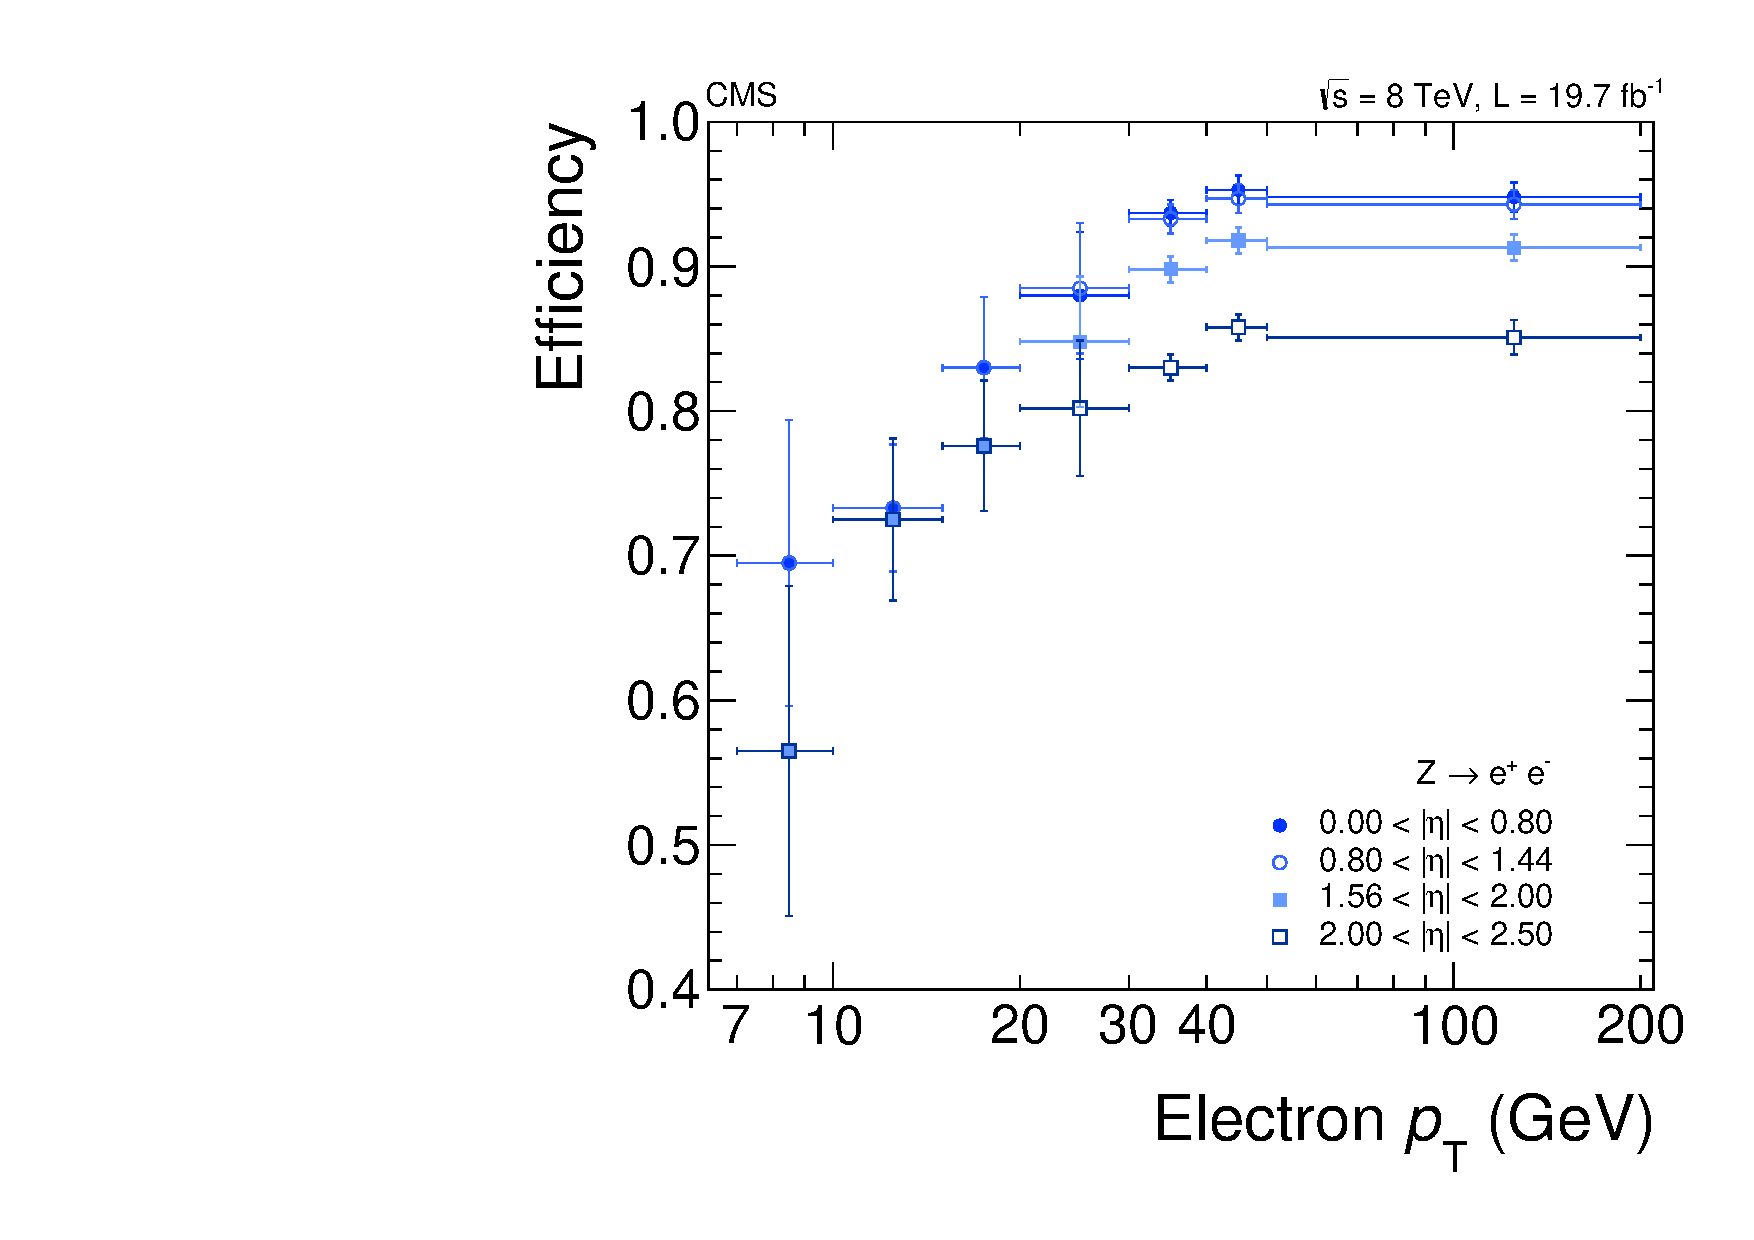
\includegraphics[width=0.45\linewidth]{{HZZ4l_search/electron_efficiency}.pdf}
      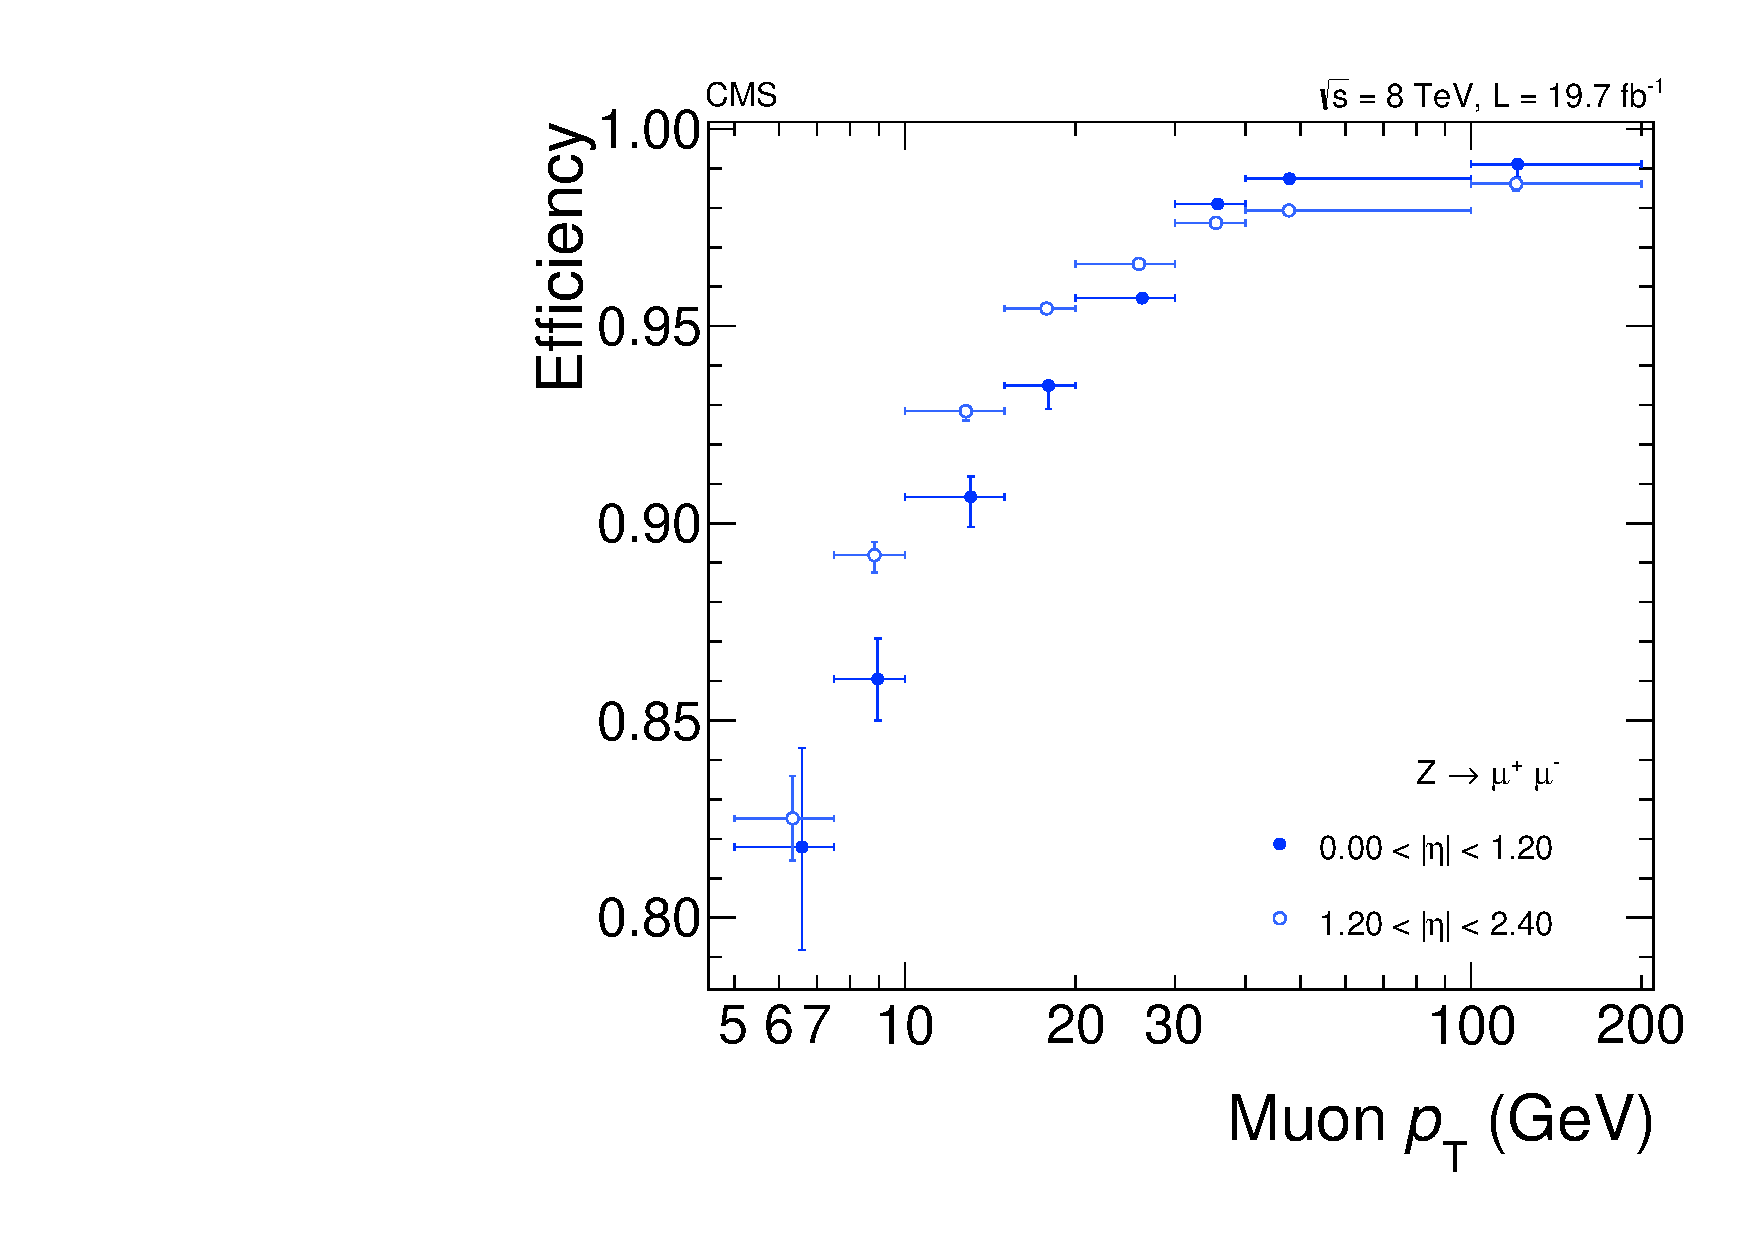
\includegraphics[width=0.45\linewidth]{{HZZ4l_search/muon_efficiency}.pdf}
    \caption[Efficiency, as a function of the lepton $p_{T}^\ell$, for
      reconstructing and selecting (left) electrons and
      (right) muons, measured with a $Z \to \ell\ell$ data sample
      by using a tag-and-probe method.]{Efficiency, as a function of the lepton $p_{T}^\ell$, for
      reconstructing and selecting (left) electrons and
      (right) muons, measured with a $Z \to \ell\ell$ data sample
      by using a tag-and-probe method \cite{Chatrchyan:2013mxa}.}
\label{fig:lepeff}
\end{center}
\end{figure}

In the analysis the presence of jets is used as an indication of vector-boson fusion (VBF) or associated production with a weak boson, $VH$, with $V$ = $W$ or $Z$, where the $V$ decays hadronically. Jets are reconstructed using the anti-$k_{T}$ clustering algorithm with distance parameter $D=0.5$, as discussed in section \ref{sec:Jets}. Jets are only
considered if they have $p_{T}^\text{jet}>\unit{30}{\GeV}$, $\abs{\eta^\text{jet}}<4.7$, originate from the primary vertex, and are required to be separated from the lepton candidates and from identified FSR photons by $\Delta R > 0.5$. Jet energy corrections are applied as a function of the jet $p_{T}^\text{jet}$ and $\eta^\text{jet}$~\cite{Chatrchyan:2011ds}. An offset correction is applied to subtract the energy contribution not associated with the high-$p_{T}$ scattering, such as electronic noise and pileup, based on the jet-area method~\cite{Chatrchyan:2011ds,Cacciari:2007fd,Cacciari:2008gn}.

\section{Event Selection, Simulation, \& Categorization}
\label{sec:Selection_Simulation_Categorizaiton}

\subsection{Simulated Data Samples}

The Monte Carlo (MC) simulated data samples, generated with state-of-the-art theoretical calculations for both the SM Higgs boson signal and relevant background processes, are used to optimize the event selection and to evaluate the acceptance and systematic uncertainties. For the gluon-gluon fusion and vector-boson fusion Higgs boson signal the simulated events are generated with \textsc{powheg} \cite{Nason:2009ai, Bagnaschi:2011tu, Frixione:2007vw} at Next-to-leading-order (NLO) QCD accuracy. The Higgs boson decay is modeled with \textsc{JHUGen} 3.1.8 \cite{Gao:2010qx, Bolognesi:2012mm, Anderson:2013afp} to include proper treatment of the interference effects associated with permutations of identical leptons in the four-electron and four-muon final states. Samples of WH, ZH, and $t\bar{t}H$ events are generated with \textsc{PYTHIA} 6.4.24 \cite{Sjostrand:2006za}. Higgs boson signal events for all production mechanisms are reweighted to include contributions from gluon fusion up to next-to-next-to-leading-order (NNLO) and next-to-next-to-leading logarithm (NNLL) \cite{Dawson1991283, Djouadi1991440, Actis:2008ug, Catani:2003zt, Ravindran:2003um, Anastasiou:2002yz, Harlander:2002wh, Spira:1995rr, Dittmaier:2011ti, Baglio:2010ae, Anastasiou:2008tj, deFlorian:2012mx}, and from the vector-boson fusion contribution computed at NNLO \cite{Dittmaier:2011ti, Ciccolini:2007jr, Ciccolini:2007ec, Figy:2003nv, Arnold:2008rz, Bolzoni:2010xr}.

The two dominant irreducible background contributions for this analysis are the SM $q\bar{q} \to ZZ$ and $gg \to ZZ$ events. The $q\bar{q} \to ZZ$ background is simulated at NLO using the \textsc{powheg} \cite{Melia:2011tj} program while the $gg \to ZZ$ contribution is simulated at LO using \textsc{GG2ZZ} \cite{Binoth:2008pr}. The yields for these SM congribitons are calculated with \textsc{MCFM} \cite{Campbell:2011bn, Campbell:1999ah, Campbell:2010ff}. The reducible backgrounds including, $Zb\bar{b}$, $Zc\bar{c}$, $Z\gamma + \text{jets}$, $WW + \text{jets}$, $WZ + \text{jets}$, etc. (referred to as $Z + \text{jets}$) are simulated with \textsc{MADGRAPH} \cite{Alwall:2007st} and used to cross check the data driven methods outlined in the next section (The $t\bar{t}$ contribution to this background is simulated at NLO with \textsc{POWHEG}).

To model the constituents (quarks \& gluons) of the colliding protons correctly, parton distributions functions are used (\textsc{CTEQ6L} \cite{Lai:2010nw} for LO generators, \textsc{CT10} \cite{Lai:2010vv} for NLO and higher-order generators). To model the underlying event, jet fragmentation, and showering all events are processed with \textsc{PYTHIA} 6.4.24 \cite{Sjostrand:2006za}. The CMS detector is simulated with great detail using a simulation based on \textsc{GEANT4} \cite{Agostinelli2003250, Allison:2006ve}.

\subsection{Selection \& Categorization}

The event selection is designed to give a set of signal candidates in the $H \to ZZ \to 4\ell$ final state in three mutually exclusive subchannels: $4e$, $4\mu$, and $2e2\mu$. Four well-identified and isolated leptons are required to originate from the primary vertex to suppress the $Z + \text{jets}$ and $t\bar{t}$ backgrounds.

Z candidates are formed with a pair of leptons of the same flavor and opposite charge $\left(\ell^{+}\ell^{-}\right)$. When forming the Z-boson candidates, only FSR photons that make the lepton-pair mass closer to the nominal Z-boson mass are incorporated. If the $m_{\ell\ell\gamma}>\unit{100}{\GeV}$, the photon is not considered, to minimize the fraction of misidentification. 

Among all the possible opposite-charge lepton paris in the event, the one with an invariant mass closest to the nominal Z-boson mass is denoted $Z_{1}$ and retained if $40 < m_{Z_{1}} < \unit{120}{\GeV}$. Then, all remaining leptons are considered and a second same flavor opposite-charge pair $\ell^{+}\ell^{-}$ becomes $Z_{2}$ when the pair has the highest scalar sum of $p_{T}^{\ell\ell}$ in the event and $12 < m_{Z_2} <\unit{120}{\GeV}$. This selection procedure results in one or more of the Z-bosons to be off shell for $m_{H} < \unit{180}{\GeV}$. 

Among the four selected leptons forming the $Z_1$ and the $Z_2$,
at least one lepton is required to have $p_{T}^\ell > \unit{20}{\GeV}$, and
another one is required to have $p_{T}^\ell > \unit{10}{\GeV}$.  These
$p_{T}^\ell$ thresholds ensure that the selected events have leptons on
the efficiency plateau of the trigger.  To further remove events with
leptons originating from hadron decays produced by jet fragmentation
or from the decay of low-mass hadron resonances, it is required that
any opposite-charge pair of leptons chosen among the four selected
leptons (irrespective of flavor) satisfy $m_{\ell^+\ell^-} > \unit{4}{\GeV}$.
The phase space for the search of the SM Higgs boson is defined by
restricting the measured mass range to $m_{4\ell} > \unit{100}{\GeV}$.

The efficiency versus $m_{H}$ is shown in Fig.~\ref{fig:effMH} for the gluon fusion Higgs boson production mode, and it is very similar for other production modes. The efficiency within the geometrical acceptance is $\approx$30\%~(58\%),
43\%~(71\%), and 62\%~(87\%) for the $4e, 2e2\mu, \text{ and } 4\mu$ channels, respectively, for $m_H = \unit{126(200)}{\GeV}$.

\begin{figure}
  \begin{center}
    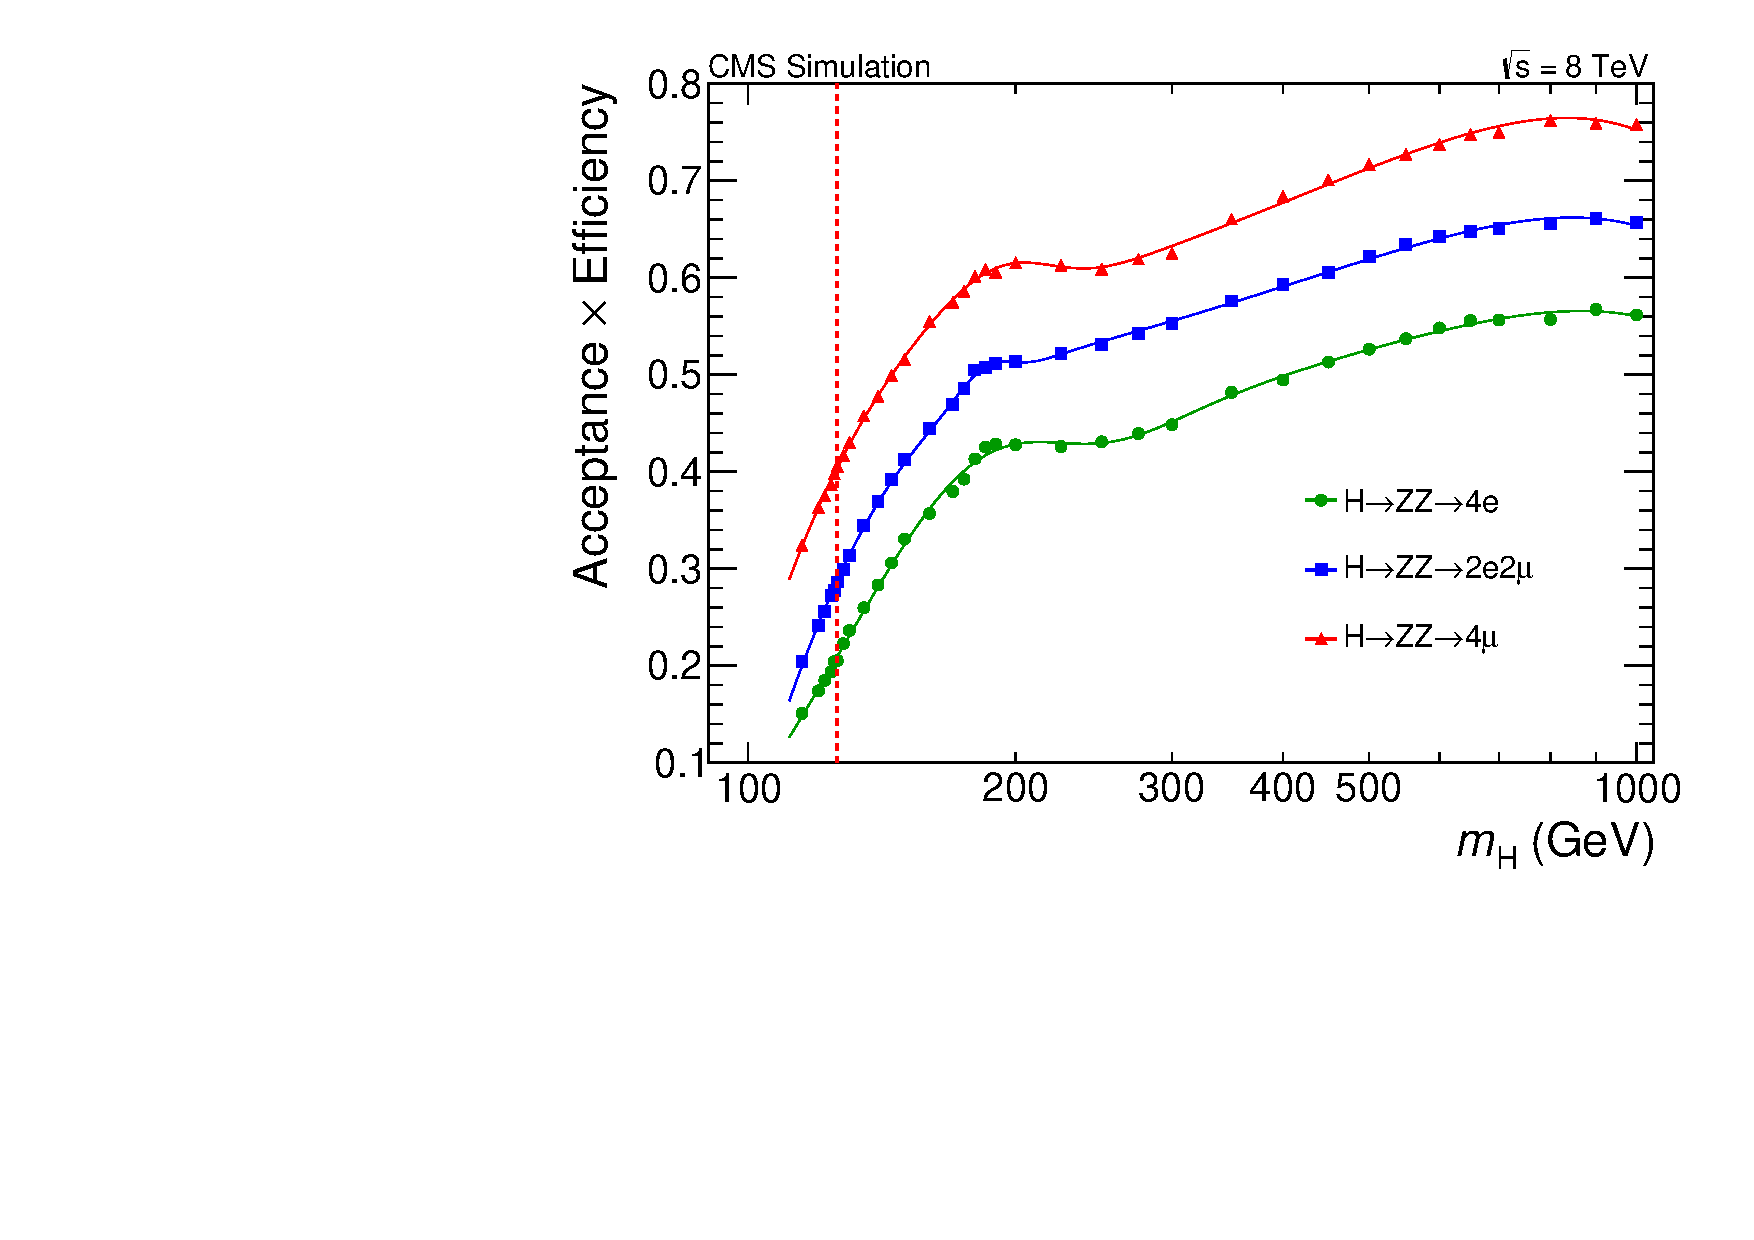
\includegraphics[width=0.65\textwidth]{HZZ4l_search/Efficiency_ggH_8TeV.pdf}
    \caption[Geometrical acceptance times selection efficiency for the SM Higgs boson signal as a function of $m_H$ in the three final states for gluon fusion production. Points represent efficiency estimated from full CMS simulation; lines represent a smooth polynomial curve interpolating the points, used in the analysis. The vertical dashed line represents $m_H = \unit{126}{\GeV}$.]{Geometrical acceptance times selection efficiency for the SM Higgs boson signal as a function of $m_H$ in the three final states for gluon fusion production. Points represent efficiency estimated from full CMS simulation; lines represent a smooth polynomial curve interpolating the points, used in the analysis. The vertical dashed line represents $m_H = \unit{126}{\GeV}$ \cite{Chatrchyan:2013mxa}.}
      \label{fig:effMH}
\end{center}
\end{figure}

In order to improve the sensitivity to the Higgs boson production mechanisms, the event sample is split into two categories based on the jet multiplicity. These categories are defined as the 0/1-jet category, containing events with fewer than two jets, and the dijet category, containing events with at least two jets.

\subsection{Background estimation}
\label{sec:BkgEstimation}

The dominant background contribution in the $H \to ZZ \to 4\ell$ search is irreducible and is due to direct ZZ production via $q\bar{q}$ annihilation and gluon fusion. The remaining subleading contributions arise from reducible multilepton sources, $Z + \text{jets}$, $t\bar{t}$, and $WZ + \text{jets}$.

The expected yield and shape of the $q\bar{q} \to ZZ$ and $gg \to ZZ$ background is evaluated using the simulated events discussed above. The $gg \to ZZ$ contribution with respect to the $q\bar{q} \to ZZ$ varies from about $2\%$ at $m_{4\ell} = \unit{126}{\GeV}$ to $6\%$ at $m_{4\ell} = \unit{1}{\TeV}$. These two background processes make up a huge fraction of the total background in this analysis. In the region $100 < m_{4\ell} < \unit{1000}{\GeV}$ is approximately $91\%, 94\%,\text{ and } 97\%$ in the $4e, 2e2\mu, \text{ and } 4\mu$ decay channels, respectively. Within the smaller range around the observed peak $\left(121.5 < m_{4\ell} < \unit{130.5}{\GeV}\right)$ these irreducible backgrounds contribute $58\%, 71\%,\text{ and } 86\%$, respectively.

The Reducible background from $Z + \text{jets}$ is estimated using two independent methods. These methods use dedicated control regions in data where there is a dilepton pair satisfying all the requirements of a $Z_{1}$ candidate and two additional leptons satisfying certain relaxed identification requirements. In both methods, the extrapolation from the control region to the signal regions is performed using the lepton misidentification probability, $f\left(\ell,p_{T}^{\ell},\abs{\eta^{\ell}}\right)$, which is defined as the fraction of non-signal leptons identified in the analysis selection criteria evaluated on a sample of enriched non-genuine electrons and muons.

The first method uses two control regions that have a $Z_{1}$ candidate and two additional leptons with the same flavor and opposite charge. There are two categories of events that satisfy the criteria, 2P2F (composed of two leptons that pass selection and two that fail the selection criteria) and 3P1F (composed of three leptons that pass selection and one that fails). For each event $i$ that falls into the 2P2F or 3P1F category a weight factor of $\frac{f_{3}^{i}}{1- f_{3}^{i}}\frac{f_{4}^{i}}{1- f_{4}^{i}}$ or $\frac{f_{a}^{i}}{1- f_{a}^{i}}$ for the third and/or fourth leptons. The 3P1F region will also have a contribution from the reducible background and so the contribution is reduced by a factor of $\left(1 - \frac{n_{3P1F}^{ZZ}}{N_{3P1F}}\right)$ where $n_{3P1F}^{ZZ}$ is the estimation of irreducible ZZ events and $N_{3P1F}$ is the total number of events in the 3P1F region. The contribution of the 2P2F to the 3P1F is also accounted for and in the end the reducible background estimation in the signal region, $N_{SR}^{reducible}$, is given by equation \eqref{eq:PredictionSR},

\begin{equation}
  \label{eq:PredictionSR}
  N^\text{reducible}_\mathrm{SR} =
  \left( 1 - \frac{n^{ZZ}_\mathrm{3P1F}}{N_\mathrm{3P1F}} \right)
  \sum_j^{N_\mathrm{3P1F}} \frac{f^j_a}{1-f^j_a}-
  \sum_i^{N_\mathrm{2P2F}} \frac{f^i_3}{1-f^i_3} \frac{f^i_4}{1-f^i_4}.
\end{equation}

The second method uses a control region that has a $Z_{1}$ candidate and two additional leptons with the same flavor and the same charge. This method exploits the linear dependence of the $f\left(\ell,p_{T}^{\ell},\abs{\eta^{\ell}}\right)$ probability on the fraction of loose electrons with tracks have one missing hit in the pixel detector $r_{\text{miss}}\left(p_{T}^{e},\abs{\eta^{e}}\right)$, which is indicative of a possible FSR photon conversion. This $r_{\text{miss}}$ fraction is estimated using samples with different FSR contributions and the $f\left(\ell,p_{T}^{\ell},\abs{\eta^{\ell}}\right)$ is corrected to ${\tilde f}\left(\ell,p_{T}^{\ell},\abs{\eta^{\ell}}\right)$ using the corresponding $r_{\text{miss}}$ fraction.
The expected number of reducible background events in the signal region is given by equation \eqref{eq:PredictionSR_2}, where $N_{2P2F_{SS}}$ is the number of observed events in the same-sign 2P2F region. The ratio $r_\mathrm{OS/SS}$ between the number of events in the 2P2F opposite-sign and same-sign control regions is obtained from simulation.

\begin{equation}
\label{eq:PredictionSR_2}
  N^\text{reducible}_\mathrm{SR} =
  r_\mathrm{OS/SS} \, \cdot \,
  \sum_i^{N_\mathrm{2P2L_{SS}}}  \tilde f^i_3  \cdot \tilde f^i_4
\end{equation}

Both of these two reducible background estimations agree well within their statistical uncertainties. Such good agreement allows the analysis to combine the two estimations of the background together, assigning a systematic unvartainty of $20\%, 25\%, \text{ and } 40\%$ for the $4e, 2e2\mu, \text{ and } 4\mu$ decay channels, respectively. Validations of these two methods are shown in figure \ref{fig:zx}.

 \begin{figure}
 \begin{center}
   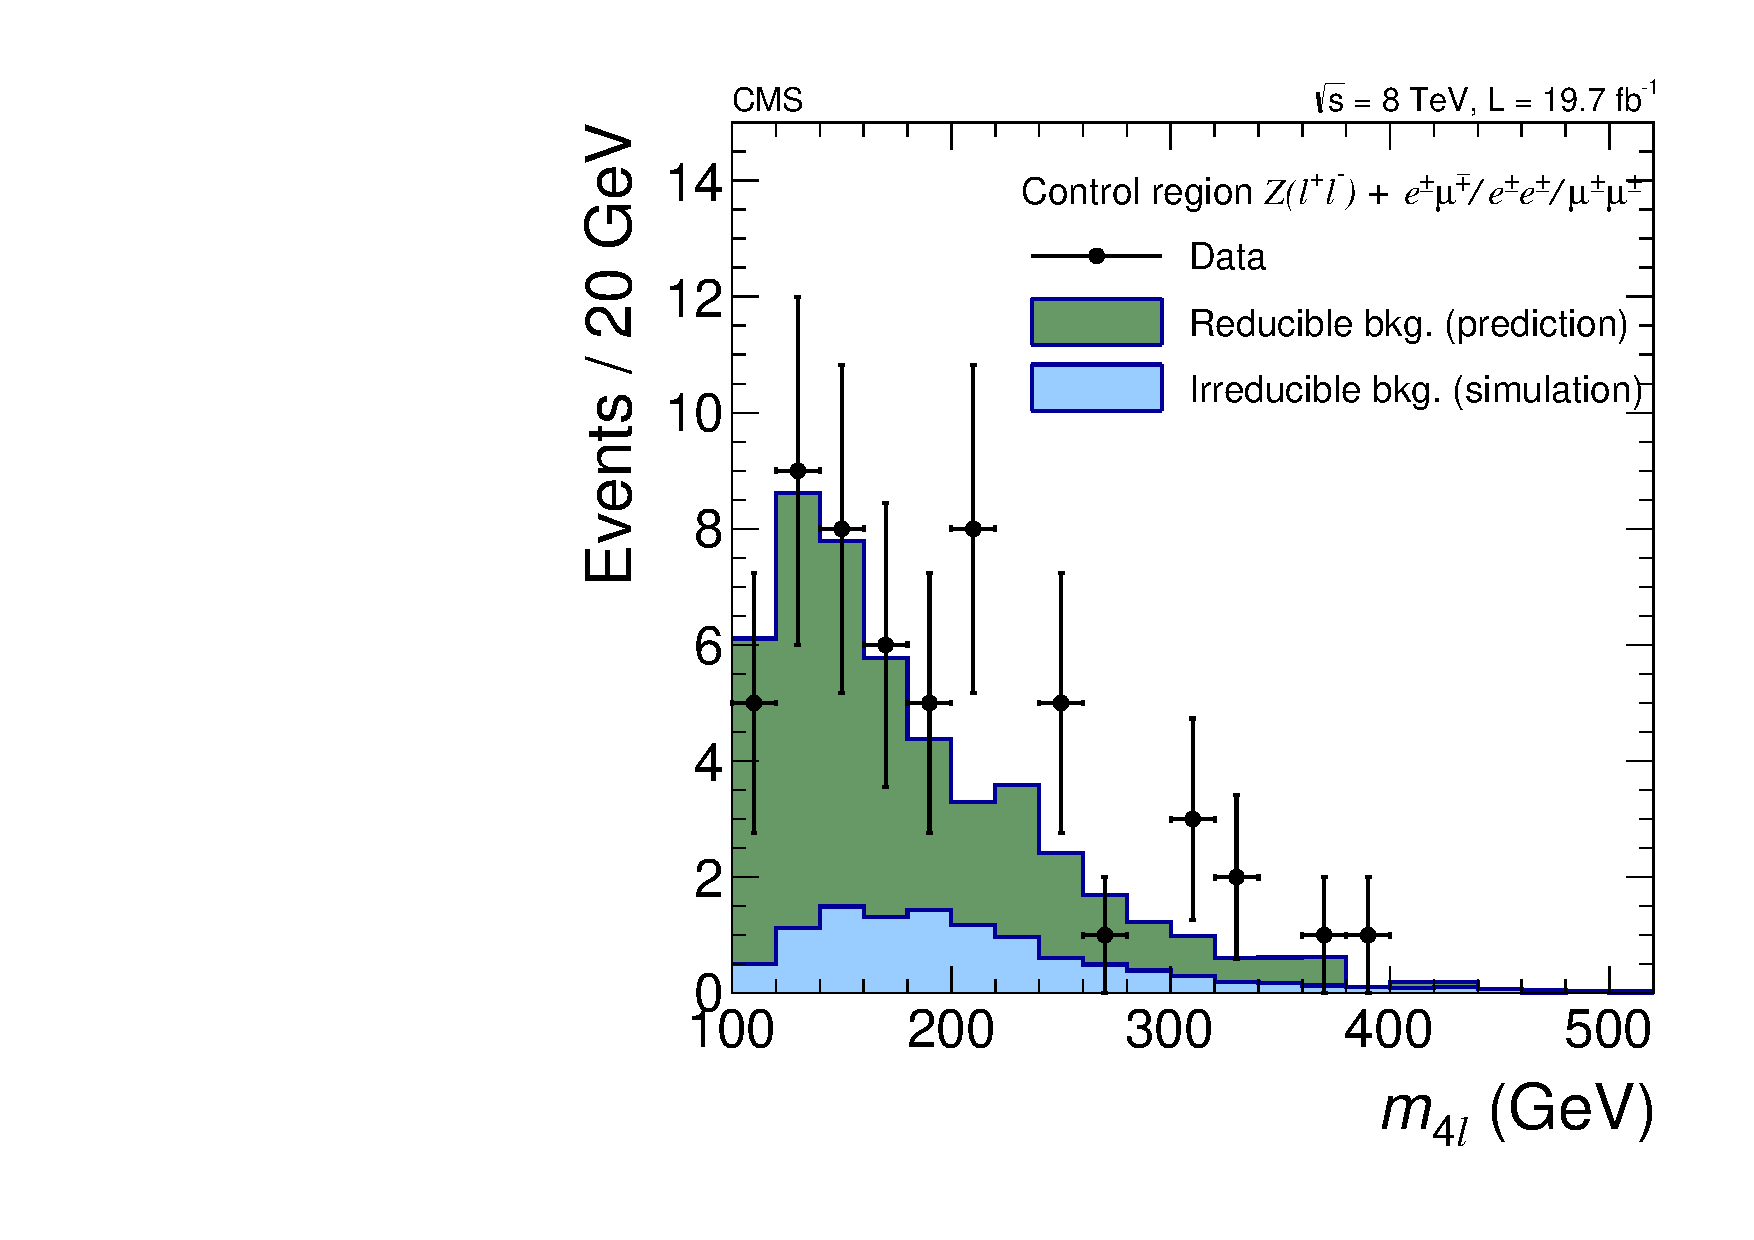
\includegraphics[width=0.45\textwidth]{HZZ4l_search/CRs_m4l_SR_4l_Prediction_WFC_PAPER.pdf}
   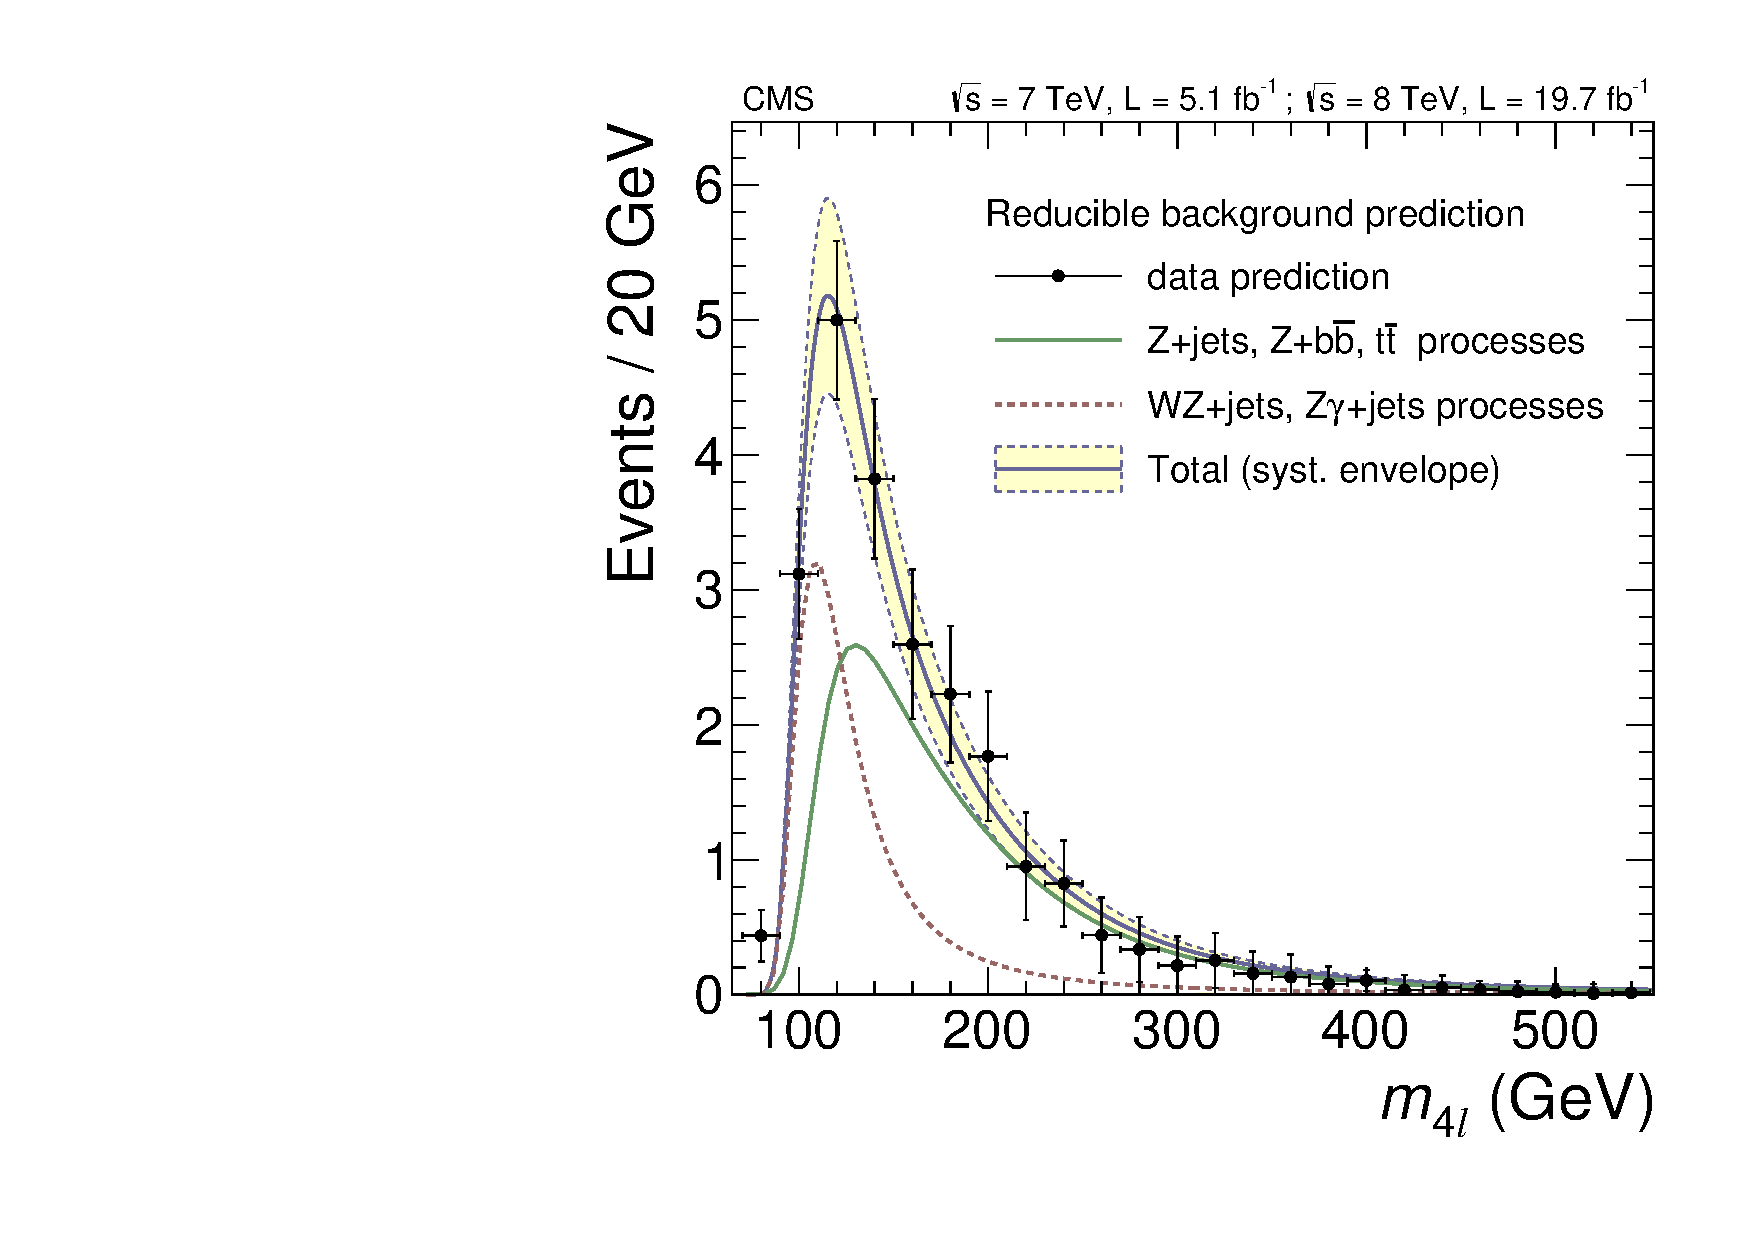
\includegraphics[width=0.45\textwidth]{HZZ4l_search/PredictedComponentsSR_withData_PAPER.pdf}
   \caption[(left) Validation of the method using the SS control
     sample. The observed $m_{4\ell}$ distribution (black dots),
     prediction of the reducible background (dark green area), and
     expected contributions from $ZZ$ (light blue area) are
     shown. (right) Prediction for the reducible background in all three
     decay channels together (black dots) fitted using an empirical shape
     (blue curve) with indicated total uncertainty (yellow band). The
     contributions from the 2P2F-like (solid green) and 3P1F-like
     (dashed red) processes are fitted separately.]{(left) Validation of the method using the SS control
     sample. The observed $m_{4\ell}$ distribution (black dots),
     prediction of the reducible background (dark green area), and
     expected contributions from $ZZ$ (light blue area) are
     shown. (right) Prediction for the reducible background in all three
     decay channels together (black dots) fitted using an empirical shape
     (blue curve) with indicated total uncertainty (yellow band). The
     contributions from the 2P2F-like (solid green) and 3P1F-like
     (dashed red) processes are fitted separately \cite{Chatrchyan:2013mxa}.
 \label{fig:zx}}
 \end{center}
 \end{figure}
 
 After all of this simulation, extrapolation, and calculation we can estimate the number of collision events we would expect to observe for the SM backgrounds and for the Higgs boson under different mass hypotheses. In the full analysis region $m_{4\ell} > \unit{100}{\GeV}$ these estimations and the statistical and systematic uncertainty on them is shown in table \ref{tab:PreFitYields}. 
 
 \begin{table}
  \begin{center}
    \caption[The number of observed candidate events compared to the
      mean expected background and signal rates for each final state.
      Uncertainties include statistical and systematic sources.  The results
      are given integrated over the full mass measurement range $m_{4\ell} >
      \unit{100}{\GeV}$ and for 7 and $\unit{8}{\TeV}$ data combined.]{The number of observed candidate events compared to the
      mean expected background and signal rates for each final state.
      Uncertainties include statistical and systematic sources.  The results
      are given integrated over the full mass measurement range $m_{4\ell} >
      \unit{100}{\GeV}$ and for 7 and $\unit{8}{\TeV}$ data combined \cite{Chatrchyan:2013mxa}.}
      \label{tab:PreFitYields}
    \begin{tabular}{lccc|c}

      Decay Channel         & $4e$ & $2e2\mu$ & $4\mu$ & $4\ell$  \\
      \hline
      $ZZ$ background  & 77  $\pm$ 10    &  191  $\pm$  25  & 119  $\pm$  15     &  387  $\pm$ 31\\
      $Z + \text{jets}$  background & 7.4 $\pm$ 1.5   & 11.5  $\pm$ 2.9  & 3.6  $\pm$ 1.5     &  22.6 $\pm$ 3.6  \\
      \hline
      All backgrounds        & 85 $\pm$ 11     & 202  $\pm$ 25    &  123  $\pm$ 15     &  410 $\pm$ 31 \\
      \hline
      $m_{H} =  \unit{500}{\GeV}$ &  5.2  $\pm$  0.6  & 12.2  $\pm$  1.4 &   7.1  $\pm$  0.8  &  24.5 $\pm$ 1.7  \\
      $m_{H} =  \unit{800}{\GeV}$ &  0.7  $\pm$  0.1  &  1.6  $\pm$  0.2 &   0.9  $\pm$  0.1  &  3.1  $\pm$ 0.2 \\
      \hline
      Observed  & 89 & 247 & 134 & 470\\
    \end{tabular}
  \end{center}
\end{table}


\section{Kinematic Distributions}
\label{sec:Kin_Dists}

Beyond counting the number of observed and expected collision events within the signal region, this analysis utilizes three kinematic distributions to separate potential signal events from background SM production. The first is the $m_{4\ell}$ shape, second is a kiematic discriminanat based on the matrix elements of both signal and background processes, the third is either the $p_{T}^{4\ell}$ or jet kinematic discriminant depending on the number of jets observed in addition to the four leptons.

\subsection{$4\ell$ mass spectrum}
\label{sec:m4l_spectrum}

The background from $ZZ$ and $Z + \text{jets}$ processes dominates after the event selection. The reconstructed four-lepton invariant mass distribution for the combined $4e, 2e2\mu,\text{ and }4\mu$ channels is shown in figure \ref{fig:Mass4l} and compared with the expectations from background processes.

\begin{figure}
\centering

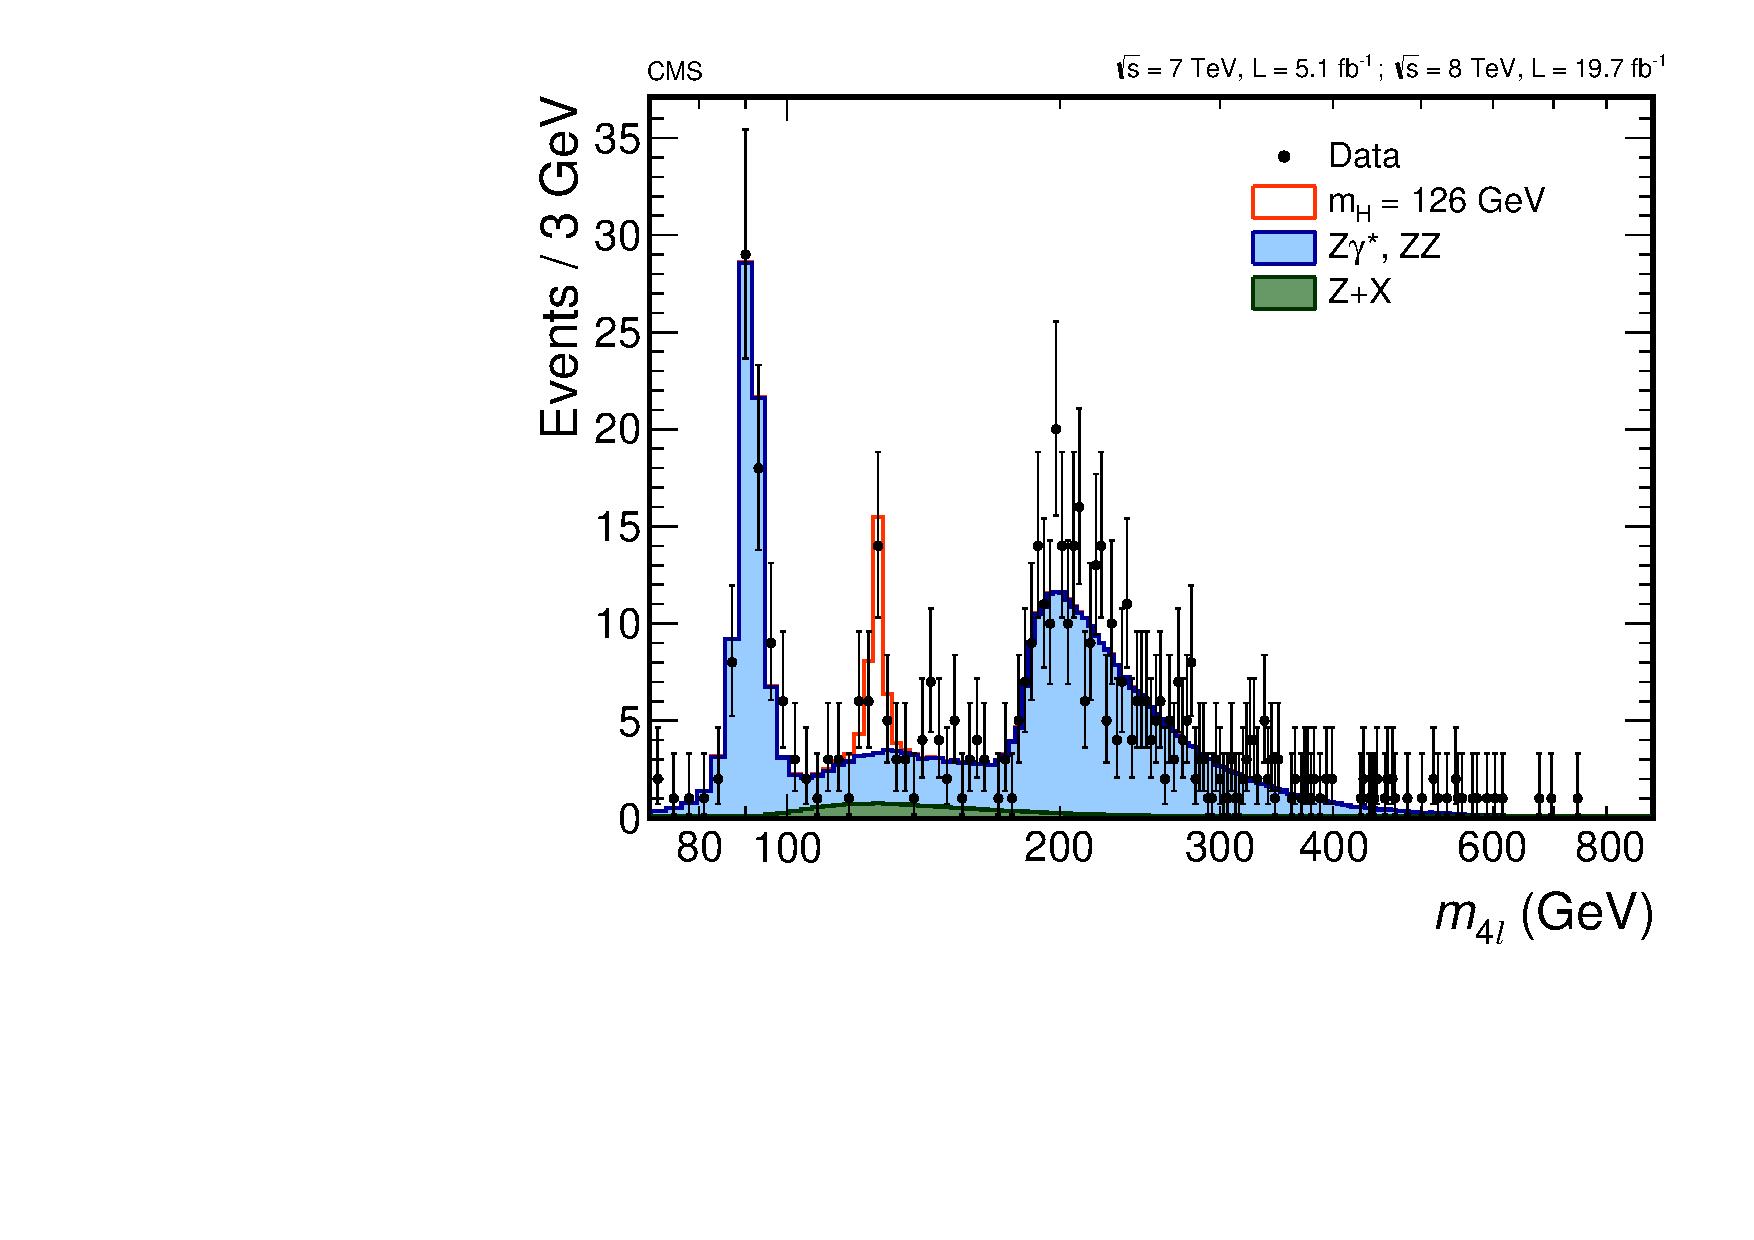
\includegraphics[width=\linewidth]{HZZ4l_search/ZZMass_7Plus8TeV_70-1000_3GeV.pdf}
\caption[Distribution of the four-lepton reconstructed mass in the
  full mass range $70<m_{4\ell}<\unit{1000}{\GeV}$ for the sum of the $4e$,
  $2e2\mu$, and $4\mu$ channels.  Points with error bars represent
  the data, shaded histograms represent the backgrounds, and the
  unshaded histogram represents the signal expectation for a mass
  hypothesis of $m_{H} = \unit{126}{\GeV}$. Signal and the $ZZ$ background are
  normalized to the SM expectation; the $Z+\text{jets}$ background to the
  estimation from data.  The expected distributions are presented as
  stacked histograms. No events are observed with
  $m_{4\ell}>\unit{800}{\GeV}$.]{ Distribution of the four-lepton reconstructed mass in the
  full mass range $70<m_{4\ell}<\unit{1000}{\GeV}$ for the sum of the $4e$,
  $2e2\mu$, and $4\mu$ channels.  Points with error bars represent
  the data, shaded histograms represent the backgrounds, and the
  unshaded histogram represents the signal expectation for a mass
  hypothesis of $m_{H} = \unit{126}{\GeV}$. Signal and the $ZZ$ background are
  normalized to the SM expectation; the $Z+\text{jets}$ background to the
  estimation from data.  The expected distributions are presented as
  stacked histograms. No events are observed with
  $m_{4\ell}>\unit{800}{\GeV}$ \cite{Chatrchyan:2013mxa}.  \label{fig:Mass4l}}

\end{figure}

The normalization and shape of the ZZ background are obtained from simulation, while the normalization of the reducible background is estimated from control samples in data, as described in section \ref{sec:BkgEstimation}. The $m_{4\ell}$ shape of the reducible background component is obtained from the opposite-sign method by fitting the $m_{4\ell}$ distributions of 2P2F and 3P1F regions separately with empirical functional forms built from Landau and exponential distributions. The systematic uncertainty in the shape is determined by the envelope that covers alternative functional forms or alternative binning.

The signal $m_{4\ell}$ shapes are also obtained from simulation. For low-mass Higgs boson hypotheses $\left(m_{H} < \unit{400}{\GeV}\right)$, the Higgs boson line shape is described with a relativistic Breit-Wigner (BW) convolved with a double-sided Crystal-Ball (CB) distribution to parameterize the reconstructed signal $m_{4\ell}$ distributions. The resulting model for the $m_{4\ell}$ peak can be seen in figure \ref{fig:4lmassmc}, where the parameterization for each final state can be seen superimposed on simulated data events. At high mass $\left(m_{H} > \unit{400}{\GeV}\right)$, the line shape is described using the complex pole scheme (CPS) \cite{Passarino:2010qk, Goria:2011wa, Kauer:2012hd}. This results in a Higgs boson width much larger than the four-lepton mass resolution. The signal parameterization for these hypotheses are modified according to this increased width instead of using the double CB functions. Systematics on the line shape are incorporated by varying the signal weights as a function of the Higgs boson mass by $\pm1\sigma$.

\begin{figure}
\centering
     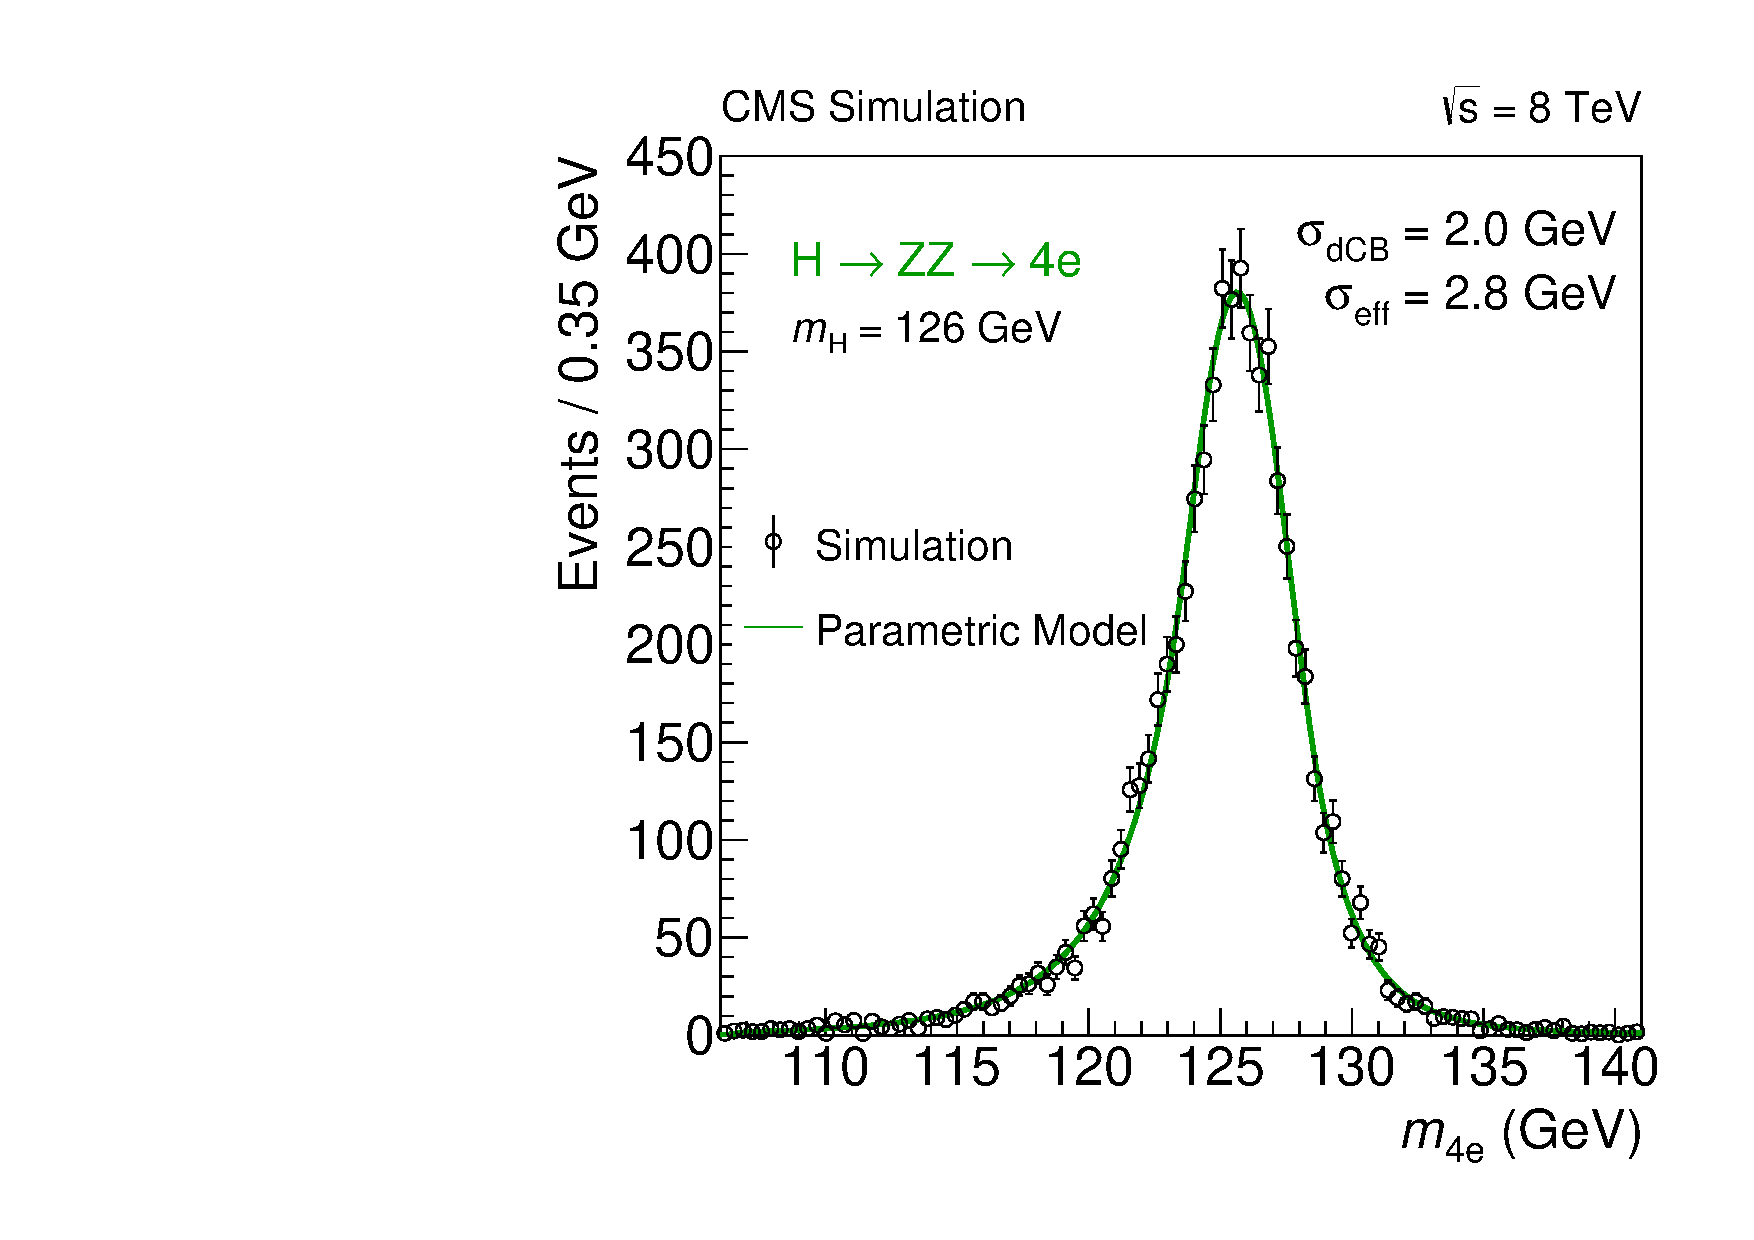
\includegraphics[width=0.32\linewidth]{HZZ4l_search/fitM126_channel1.pdf}
     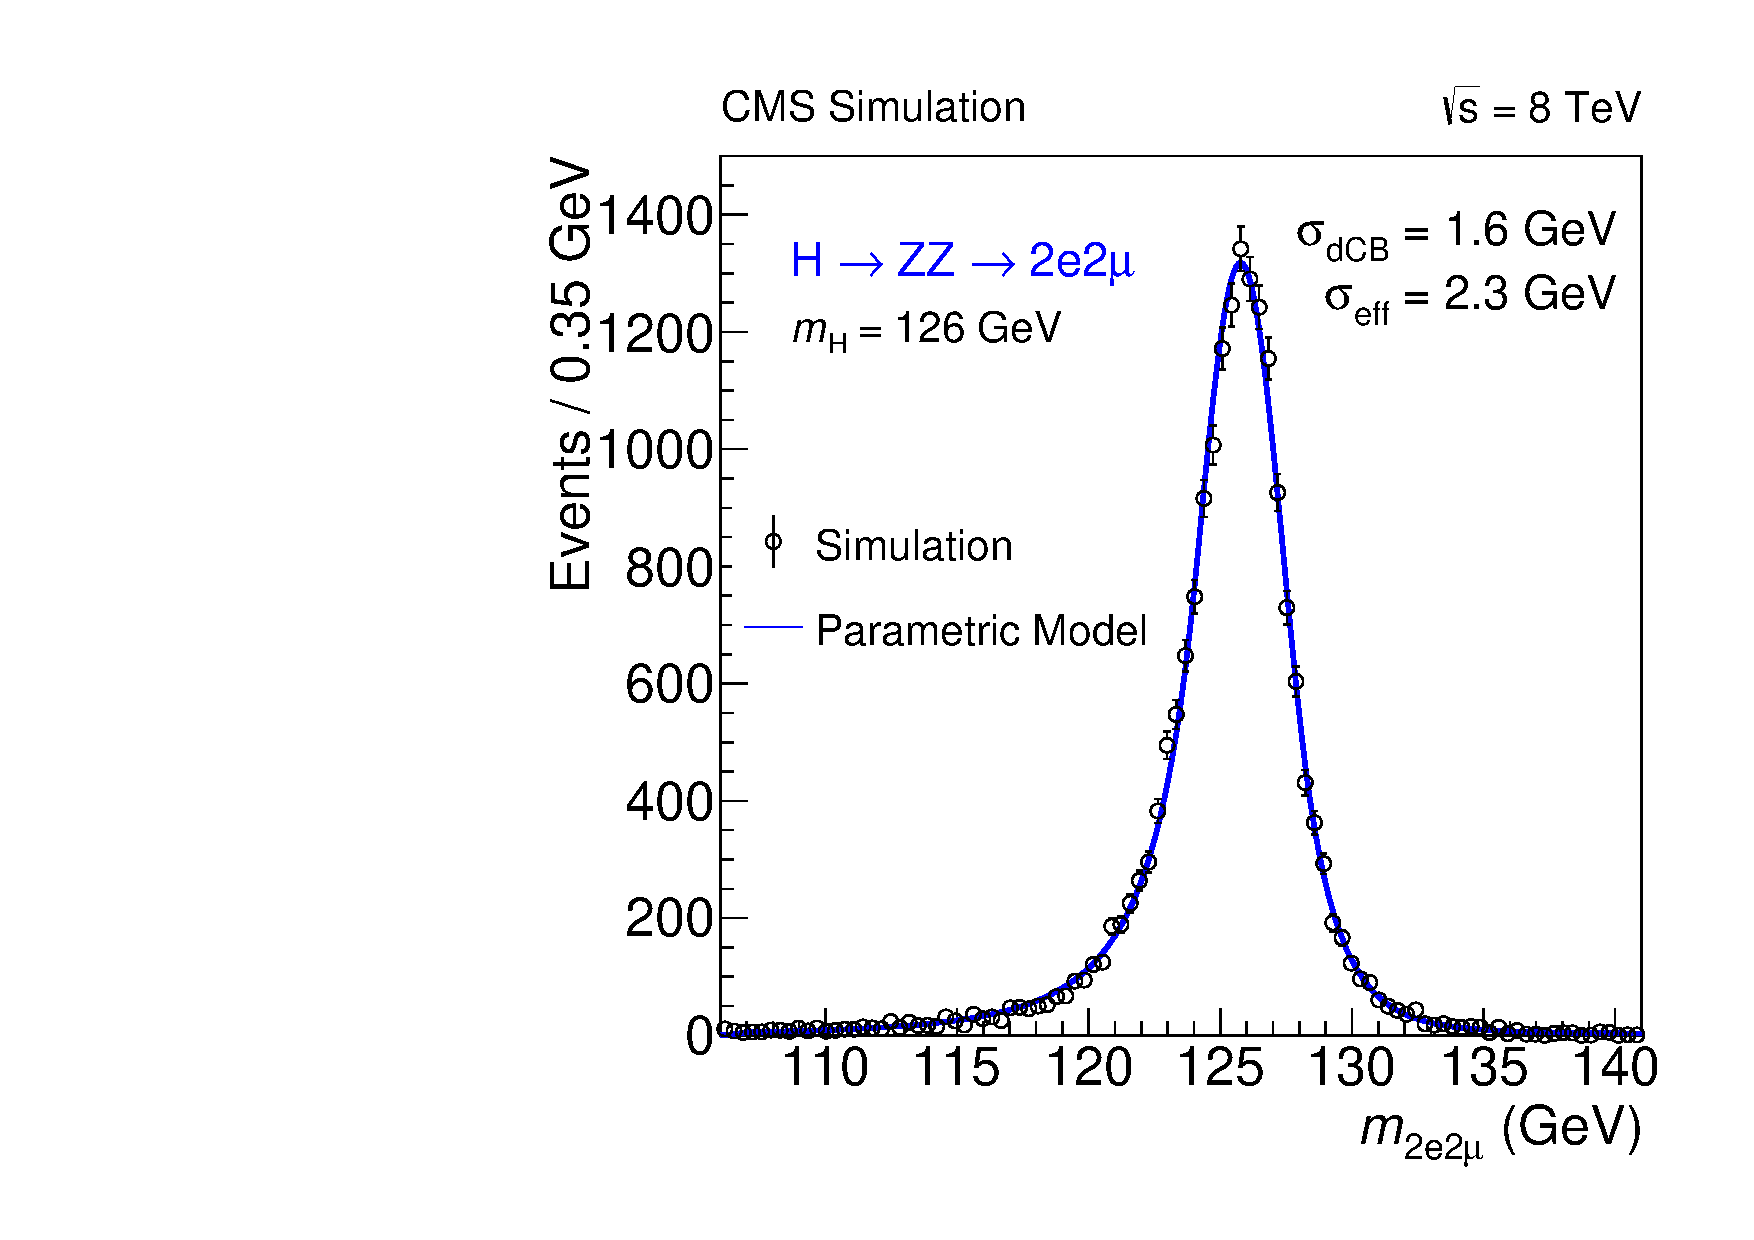
\includegraphics[width=0.32\linewidth]{HZZ4l_search/fitM126_channel2.pdf}
     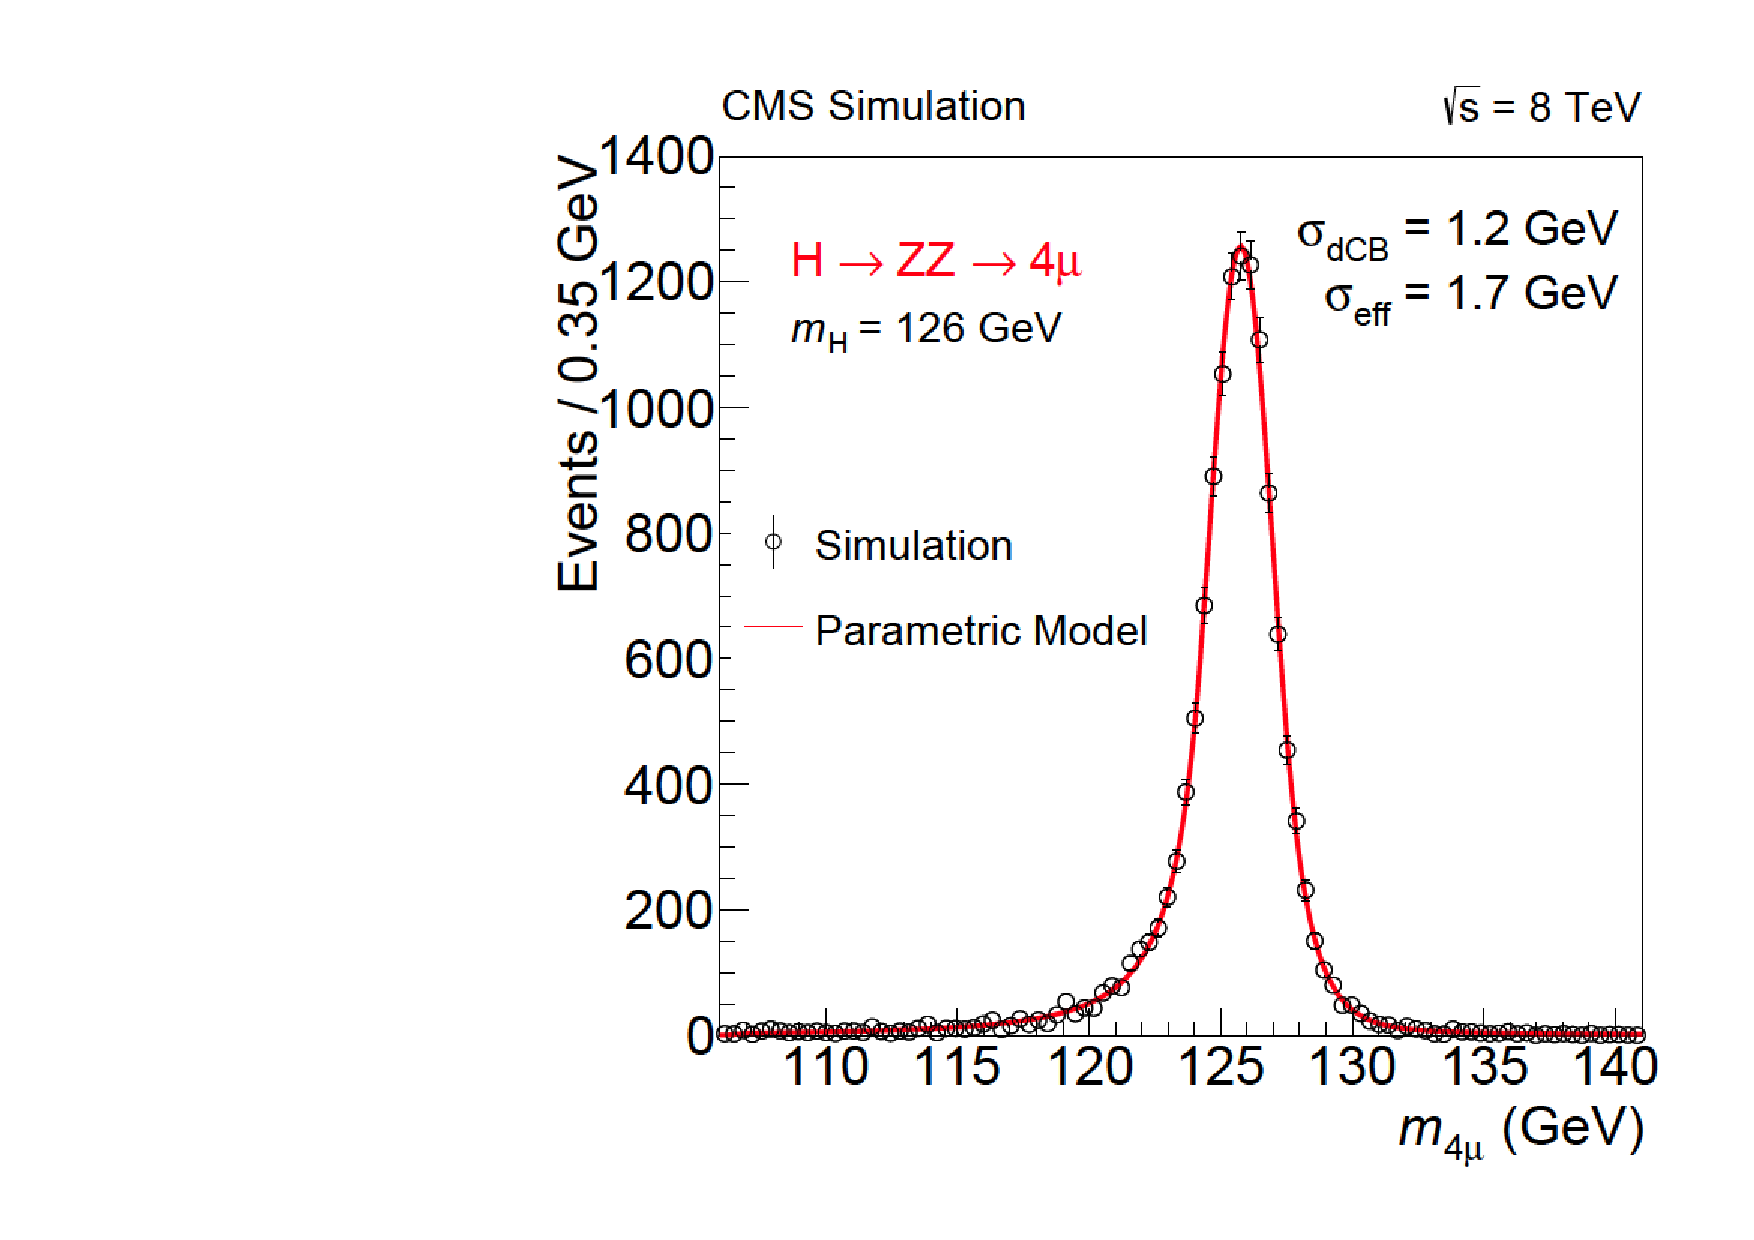
\includegraphics[width=0.32\linewidth]{HZZ4l_search/fitM126_channel0.pdf}
\caption[The $H \to ZZ \to 4\ell$ invariant mass
  distribution for $m_{H} = \unit{126}{\GeV}$ in the (left) $4e$, (center) $2e2\mu$,
  and (right) $4\mu$ channels. The distributions are fitted with a
  double-sided CB function and the fitted values of the CB width
  $\sigma_{\mathrm{dCB}}$ are indicated. The values of effective resolution,
  defined as half the smallest width that contains 68.3\% of the
  distribution, are also indicated. The distributions are arbitrarily
  normalized.]{ The $H \to ZZ \to 4\ell$ invariant mass
  distribution for $m_{H} = \unit{126}{\GeV}$ in the (left) $4e$, (center) $2e2\mu$,
  and (right) $4\mu$ channels. The distributions are fitted with a
  double-sided CB function and the fitted values of the CB width
  $\sigma_{\mathrm{dCB}}$ are indicated. The values of effective resolution,
  defined as half the smallest width that contains 68.3\% of the
  distribution, are also indicated. The distributions are arbitrarily
  normalized \cite{Chatrchyan:2013mxa}.}
\label{fig:4lmassmc}
\end{figure}


\subsection{Matrix Element Likelihood Approach (MELA) kinematic discriminant}
\label{sec:MELA}

As we have mentioned the four-lepton decay mode has the advantage that the kinematics of the Higgs boson and its decay products are all visible in the detector, providing many independent observables that can be used for different purposes. In addition to the invariant mass, the angular distributions for the four leptons and the dilepton pairs invariant masses can be used to further discriminate signal from background, increasing the sensitivity and reducing the statistical uncertainty in the observations.

Five angles $\vec{\Omega} \equiv \left(\theta^{*}, \Phi_{1}, \theta_{1}, \theta_{2}, \Phi\right)$ \cite{Gao:2010qx, Bolognesi:2012mm, Anderson:2013afp, PhysRev.168.1926} seen in figure \ref{fig:decay}  and the invariant masses of the lepton pairs $m_{Z_{1}}$ and $m_{Z_{2}}$, fully describe the kinematic configuration of a four-lepton system in its center-of-mass frame, up to an arbitrary rotation around the beam axis. These observables provide significant discriminating power between signal and background. A matrix-element likelihood approach (MELA) is used to construct a kinematic discriminant related to the decay observables \cite{Chatrchyan:2013lba, Chatrchyan:2012jja}.

\begin{figure}
\begin{center}
\centering
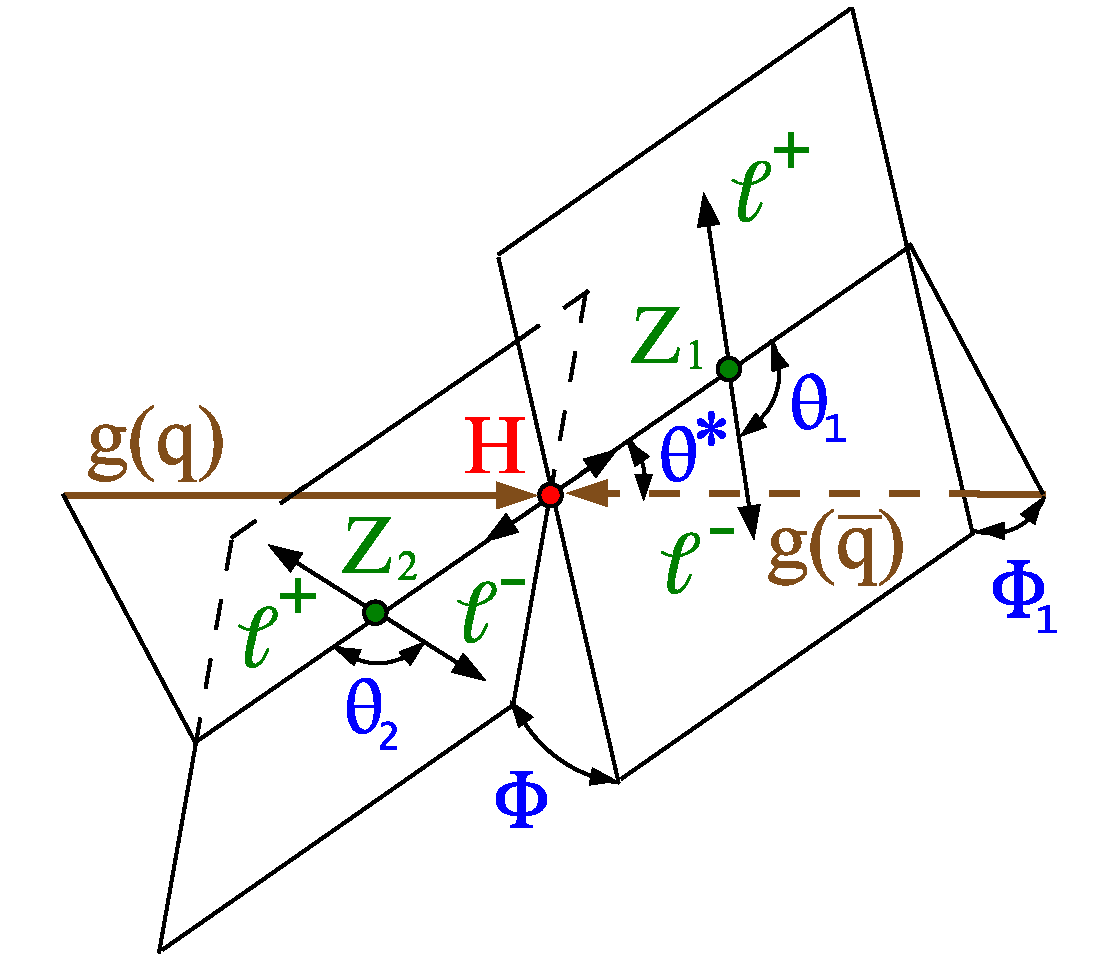
\includegraphics[width=0.45\linewidth]{HZZ4l_search/angles-HZZ4l_snowmass.pdf}
\caption[Illustration of the production and decay of a particle
  $H$, $gg(q\bar{q}) \to H \to ZZ \to 4\ell$, with the two production angles $\theta^*$ and $\Phi_1$ shown
  in the $H$ rest frame and three decay angles $\theta_1$,
  $\theta_2$, and $\Phi$ shown in the $Z_1$, $Z_2$, and $H$
  rest frames, respectively.]{ Illustration of the production and decay of a particle
  $H$, $gg(q\bar{q}) \to H \to ZZ \to 4\ell$, with the two production angles $\theta^*$ and $\Phi_1$ shown
  in the $H$ rest frame and three decay angles $\theta_1$,
  $\theta_2$, and $\Phi$ shown in the $Z_1$, $Z_2$, and $H$
  rest frames, respectively \cite{Anderson:2013afp}.
\label{fig:decay}}
\end{center}
\end{figure}

Each of these five observables carries some information about how the $4\ell$ event was produced. The distribution of these is shown in figure \ref{fig:kinematics}. This figure also shows predicted distributions for BSM bosons, which will become relevant in later sections. In principle, with enough computing power and effort one could construct an analysis that uses all of them independently. However, without loss in performance one can use the event probabilities that come from the matrix-element corresponding to a given point in phase space. This way the analysis is simplified and the correlations between these different variables are maintained.

\begin{figure}
\centering
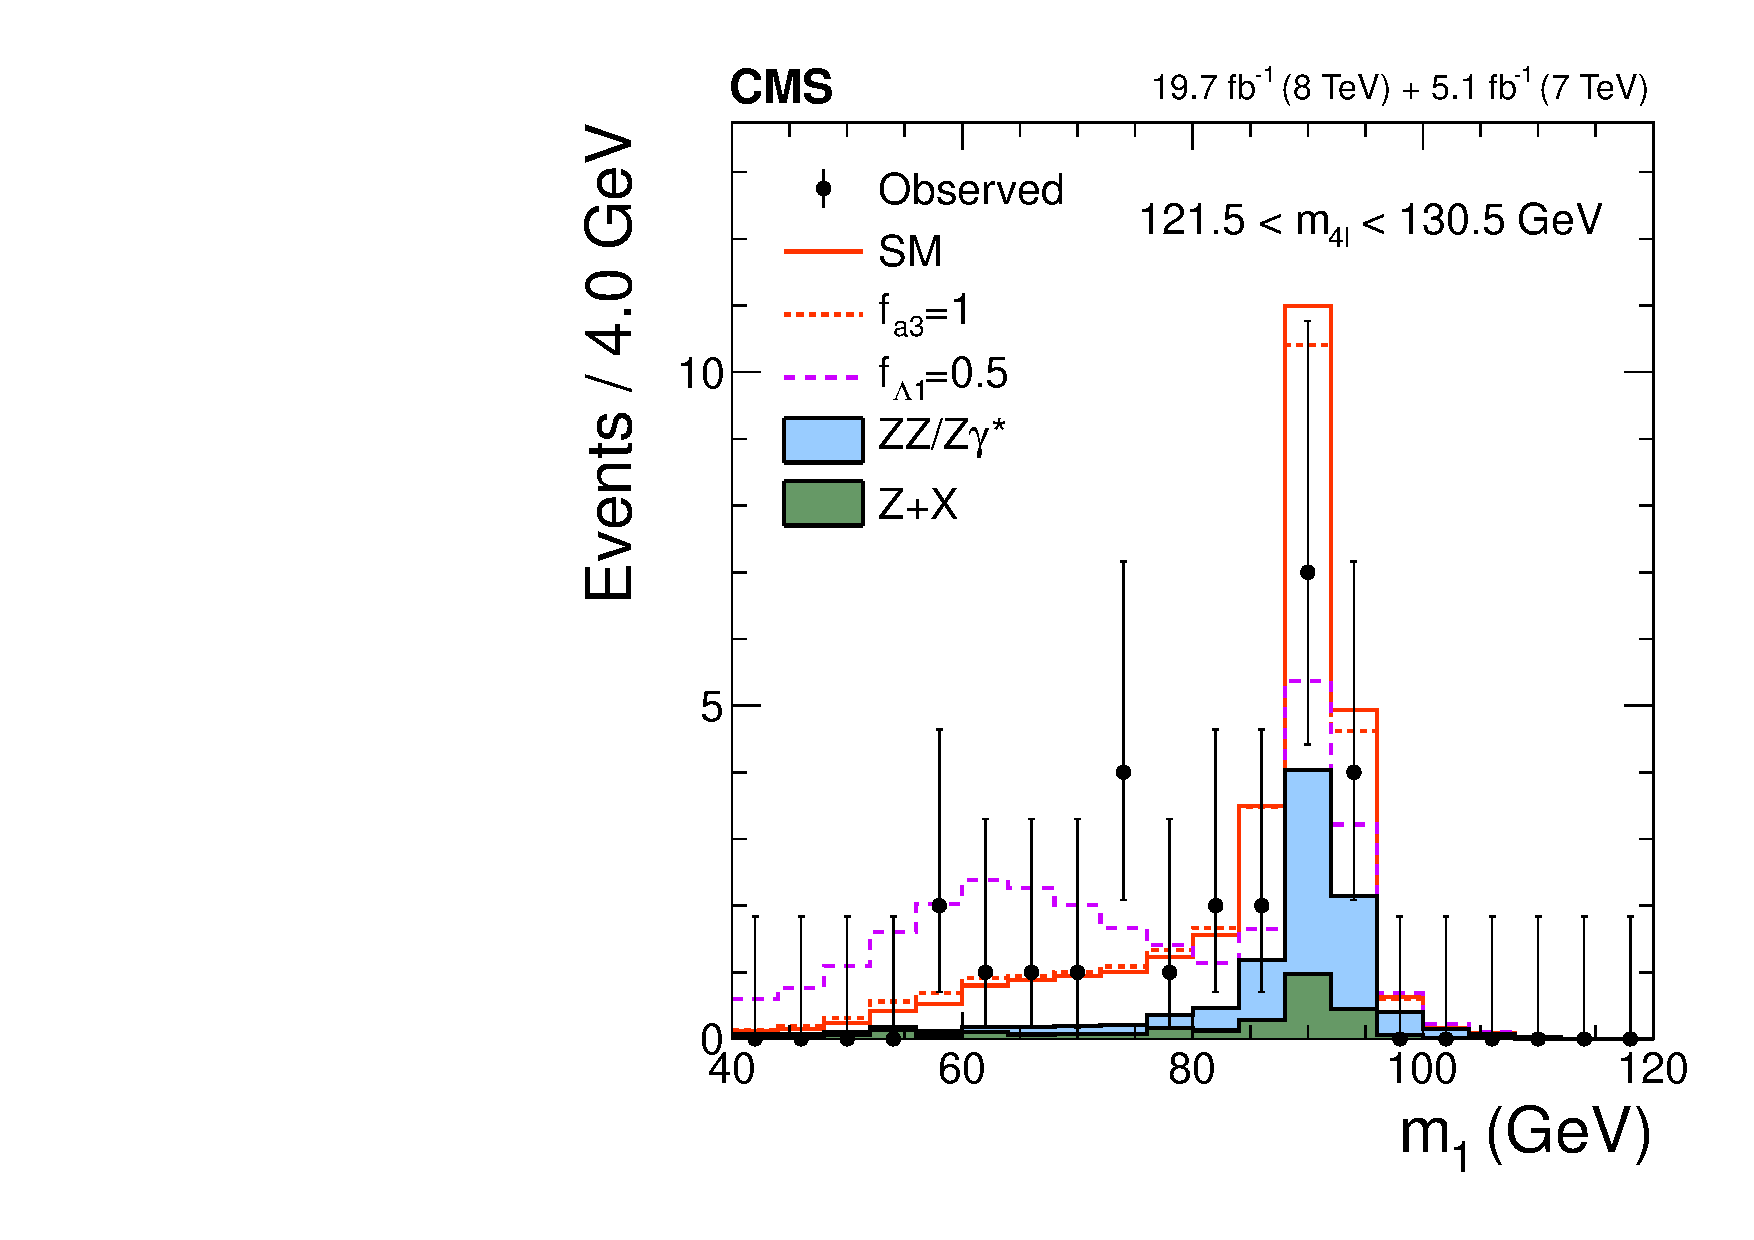
\includegraphics[width=0.32\textwidth]{HZZ4l_search/cCompare_DataMC_AllTeV_Z1Mass_SignalEnriched.pdf}
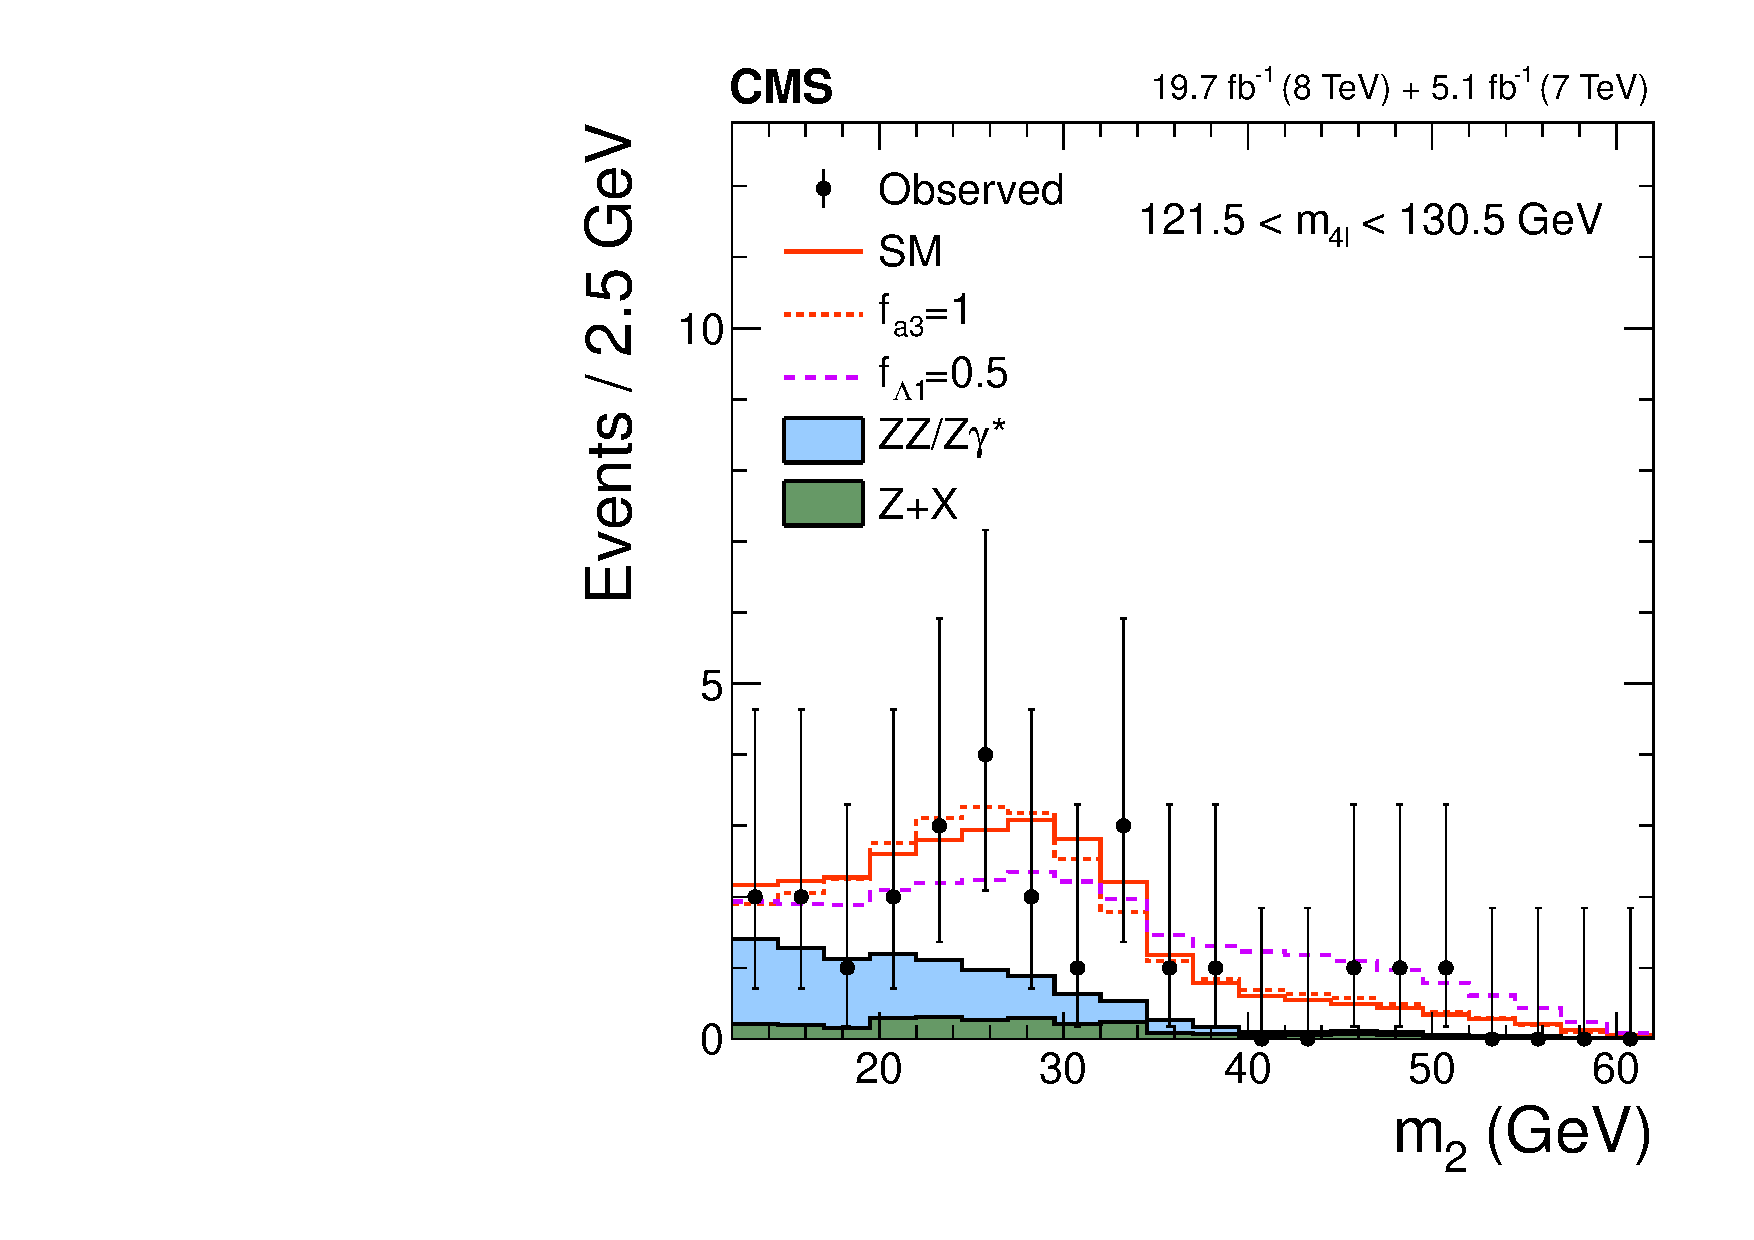
\includegraphics[width=0.32\textwidth]{HZZ4l_search/cCompare_DataMC_AllTeV_Z2Mass_SignalEnriched.pdf} \\
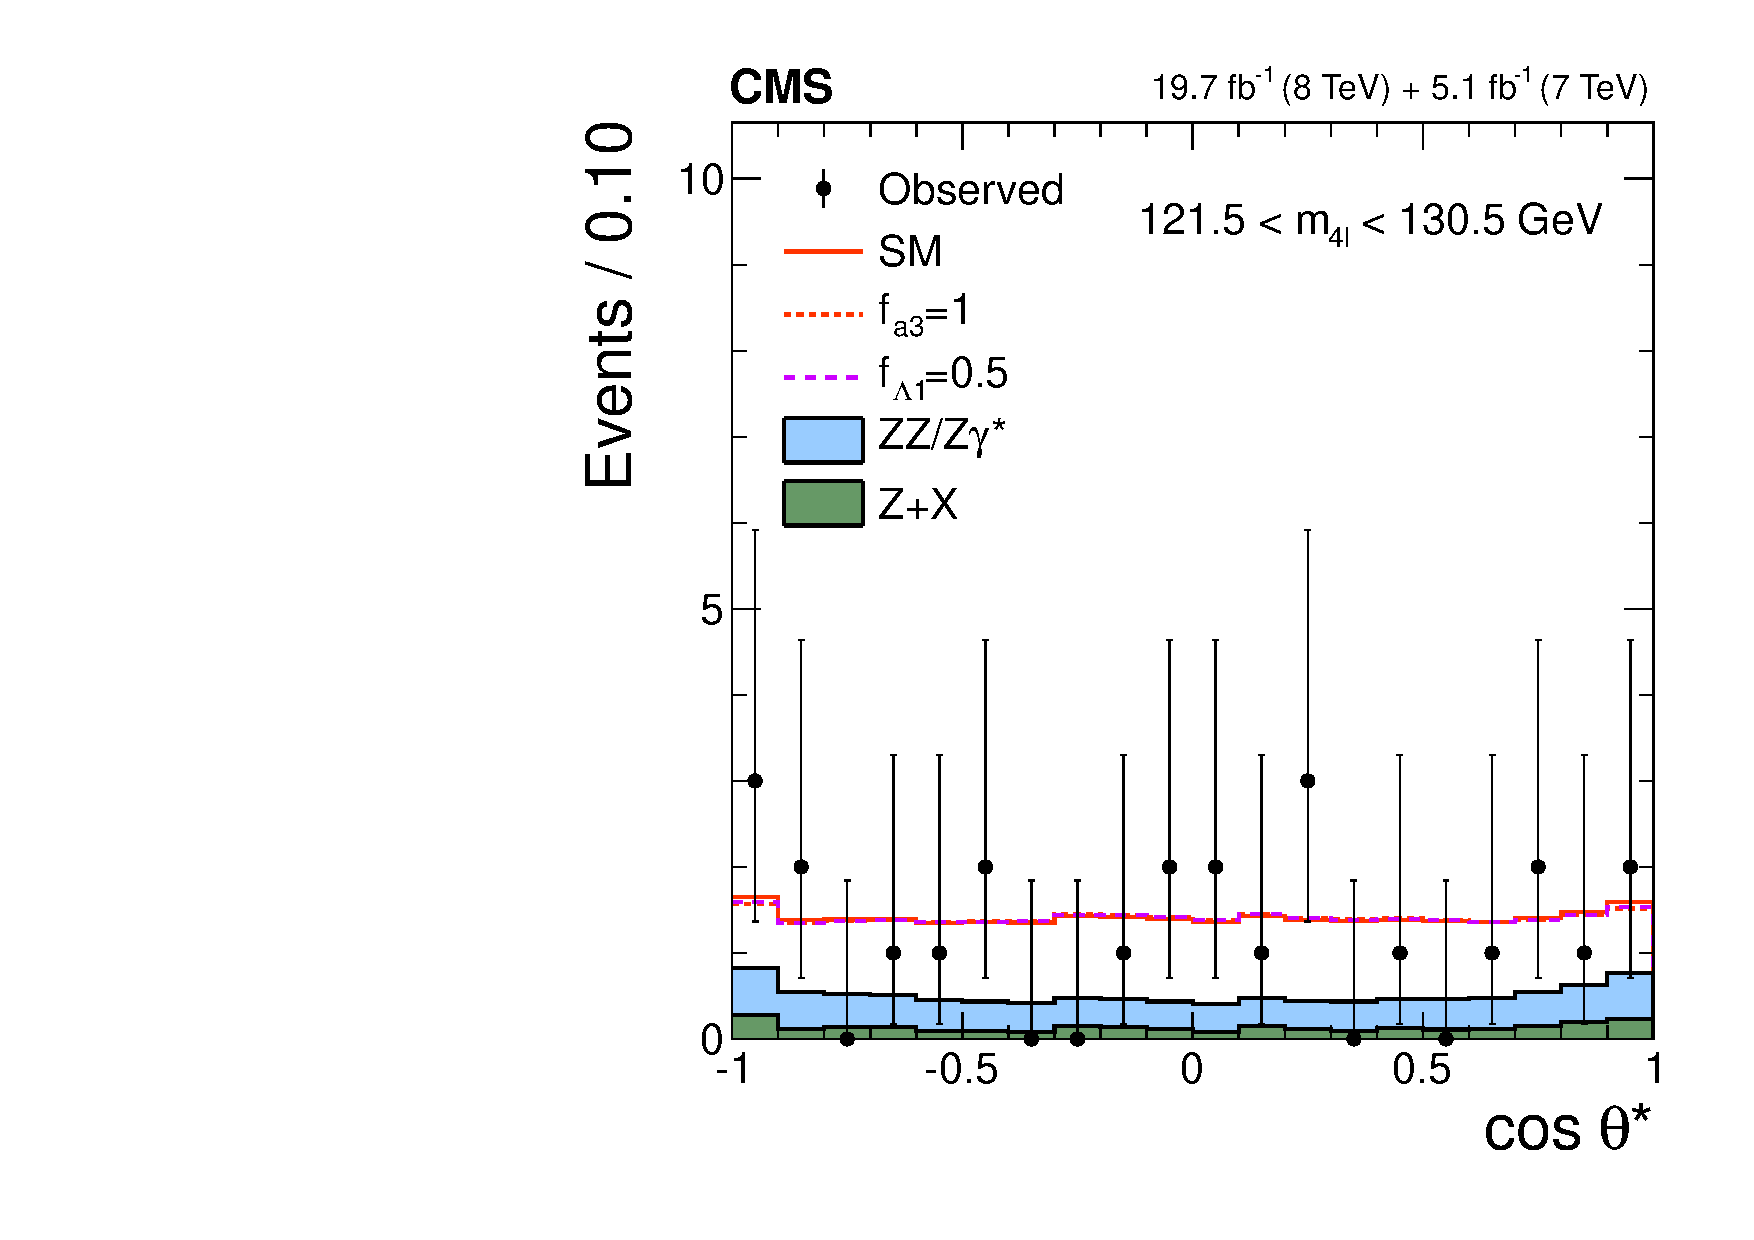
\includegraphics[width=0.32\textwidth]{HZZ4l_search/cCompare_DataMC_AllTeV_costhetastar_SignalEnriched.pdf}
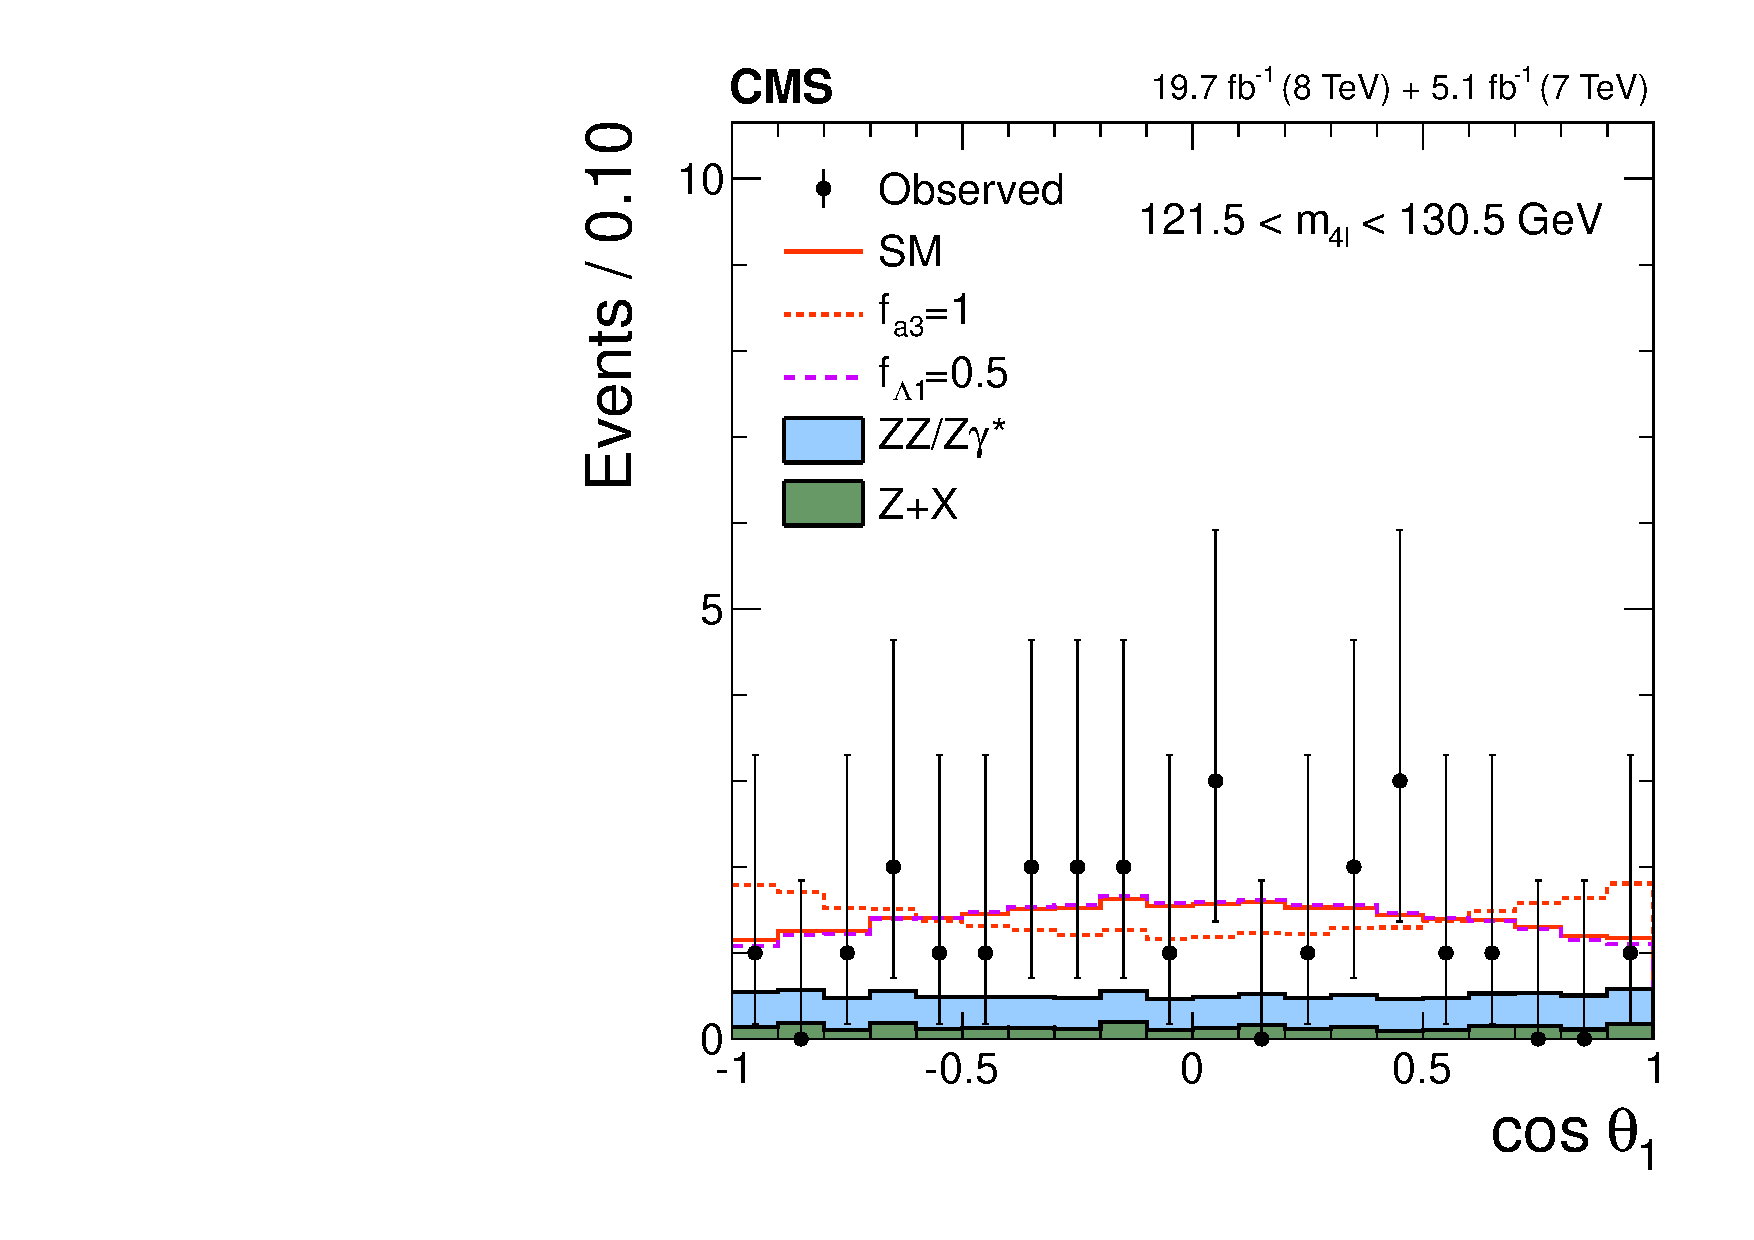
\includegraphics[width=0.32\textwidth]{HZZ4l_search/cCompare_DataMC_AllTeV_helcosthetaZ1_SignalEnriched.pdf}
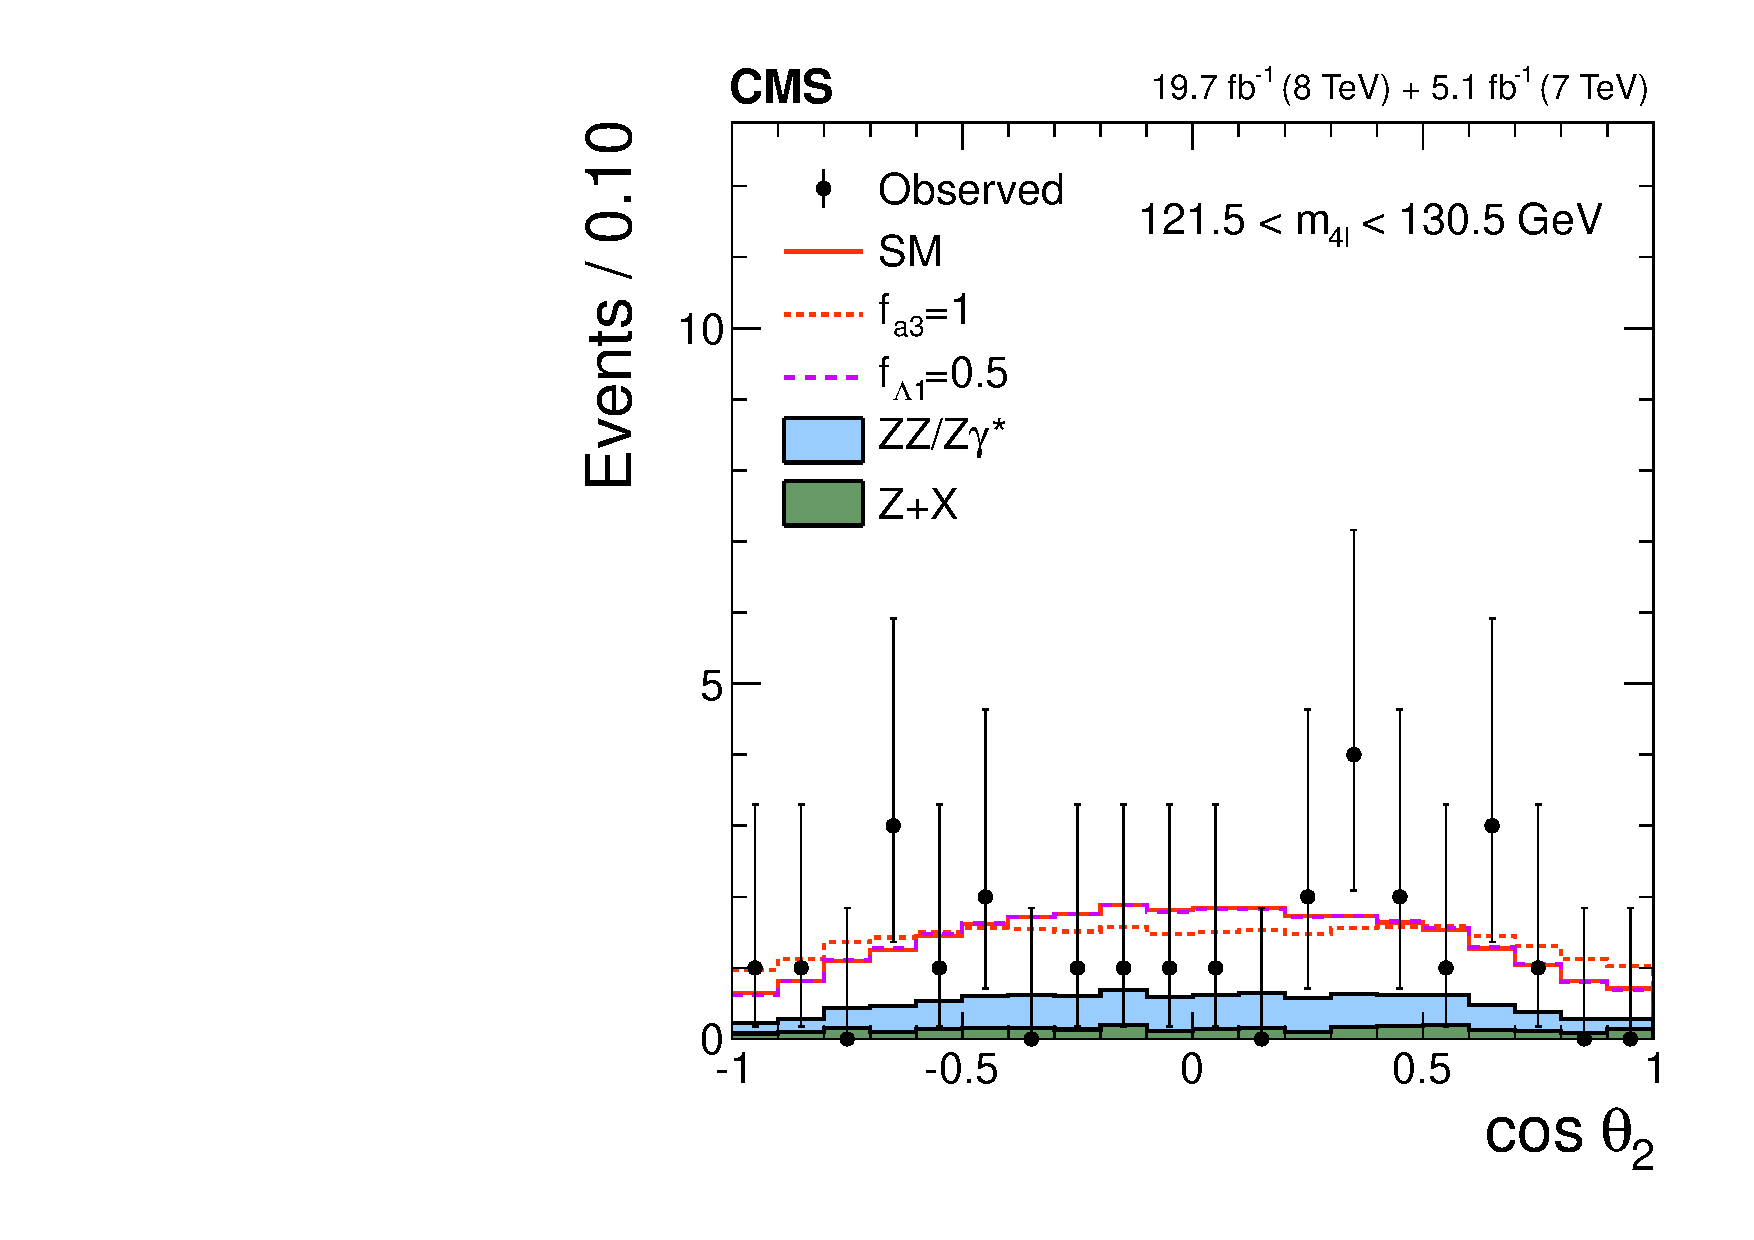
\includegraphics[width=0.32\textwidth]{HZZ4l_search/cCompare_DataMC_AllTeV_helcosthetaZ2_SignalEnriched.pdf} \\
\includegraphics[width=0.32\textwidth]{HZZ4l_search/cCompare_DataMC_AllTeV_helphi_SignalEnriched.pdf}
\includegraphics[width=0.32\textwidth]{HZZ4l_search/cCompare_DataMC_AllTeV_phistarZ1_SignalEnriched.pdf}
\caption[ Distributions of the eight kinematic observables used in the $H \to ZZ \to 4\ell$ analysis:
$m_{Z_1}$, $m_{Z_2}$, $\cos\theta^*$, $\cos\theta_{1}$, $\cos\theta_{2}$, $\Phi$, and $\Phi_{1}$.
The observed data (points with error bars), the expectations for the SM background (shaded areas),
the SM Higgs boson signal (open areas under the solid histogram),
and the alternative spin-zero resonances (open areas under the dashed histograms) are shown,
as indicated in the legend. The mass of the resonance is taken to be $\unit{125.6}{\GeV}$ and the SM cross section is used. All distributions, with the exception of $m_{4\ell}$, are presented with the requirement
$121.5 < m_{4\ell} < \unit{130.5}{\GeV}$.]{ Distributions of the eight kinematic observables used in the $H \to ZZ \to 4\ell$ analysis: $m_{Z_1}$, $m_{Z_2}$, $\cos\theta^*$, $\cos\theta_{1}$, $\cos\theta_{2}$, $\Phi$, and
$\Phi_{1}$.
The observed data (points with error bars), the expectations for the SM background (shaded areas),
the SM Higgs boson signal (open areas under the solid histogram),
and the alternative spin-zero resonances (open areas under the dashed histograms) are shown,
as indicated in the legend.
The mass of the resonance is taken to be $\unit{125.6}{\GeV}$ and the SM cross section is used.
All distributions, with the exception of $m_{4\ell}$, are presented with the requirement
$121.5 < m_{4\ell} < \unit{130.5}{\GeV}$ \cite{Khachatryan:2014kca}.}
\label{fig:kinematics}
\end{figure}

To separate a SM signal $\left(J^{P} = 0^{+}\right)$ from background a kinematic discriminant $\left(\mathcal{D}^{\text{kin}}_{\text{bkg}}\right)$ is defined based on the event probabilities $\mathcal{P}\left(m_{Z_{1}}, m_{Z_{1}}, \vec{\Omega} | m_{4\ell}\right)$ of the background or signal probability distribution of angular and mass observables computed from the LO matrix element squared for signal or ZZ processes. This discriminant is defined as in equation \eqref{eq:kd-mela}, giving the added advantage that to first order acceptance and phase space factors will cancel in the ratio. Thus, one does not need to integrate the matrix elements over the full kinematic range but simply calculate the magnitude of the matrix element squared at the point in phase space where each event appears.

The expected $\mathcal{D}^{\text{kin}}_{\text{bkg}}$ shapes for signal and the $q\bar{q} \to ZZ$ and $gg \to ZZ$ backgrounds are taken from simulation of the three decay channels $4e$, $2e2\mu$, and $4\mu$ independently. Given the low statistics and unreliable simulation of the $Z + \text{jets}$ contribution is modeled by collision events in the control regions. The statistics are boosted by merging all decay channels and control regions together using the appropriate weight to map them to the signal region. 

\begin{equation}
  \label{eq:kd-mela}
  \mathcal{D}^{\text{kin}}_{\text{bkg}} = \frac{\mathcal{P}^\text{kin}_{0^+} }{\mathcal{P}^\text{kin}_{0^+} +\mathcal{P}^\text{kin}_\text{bkg} }=
  \left[1+\frac{\mathcal{P}^\text{kin}_\text{bkg}(m_{Z_1}, m_{Z_2}, \vec\Omega | m_{4\ell})}
    {\mathcal{P}^\text{kin}_{0^+} (m_{Z_1}, m_{Z_2}, \vec\Omega | m_{4\ell})}  \right]^{-1}. \\
\end{equation}

Because these discriminant values do not directly carry $m_{4\ell}$ discrimination power they are used as a second dimensions for discrimination between signal and background. The distributions of the $\mathcal{D}^{\text{kin}}_{\text{bkg}}$ versus $m_{4\ell}$ are shown for the selected events and compared to the SM background expectation in figure \ref{fig:KDvsM4lFullMass}. The distribution of events in the $\left(m_{4\ell}, \mathcal{D}^{\text{kin}}_{\text{bkg}}\right)$ plane agrees well with the SM background expectation in the high-mass range, figure \ref{fig:KDvsM4lFullMass}~(right), while discrepancies in the two-dimensional plane are observed in the low-mass range $110<m_{4\ell}<\unit{180}{\GeV}$, figure~\ref{fig:KDvsM4lFullMass}~(left), indicative of the presence of a signal.


\begin{figure}
  \begin{center}
    \includegraphics[width=0.45\textwidth]{HZZ4l_search/KD_vs_m4l_lowMass_Back.pdf}
    \includegraphics[width=0.45\textwidth]{HZZ4l_search/KD_vs_m4l_highMass_Back.pdf}
    \caption[Distribution of the kinematic discriminant $\mathcal{D}^{\text{kin}}_{\text{bkg}}$ versus
      the four-lepton reconstructed mass $m_{4\ell}$ in the (left)
      low-mass and (right) high-mass regions.  The color scale represents
      the expected relative density in linear scale (in arbitrary
      units) of background events.  The points show the data and the
      measured per-event invariant mass uncertainties as horizontal
      bars. One $2e2\mu$ event with $m_{4\ell}\approx \unit{220}{\GeV}$ and
      small $\mathcal{D}^{\text{kin}}_{\text{bkg}}$ has a huge mass uncertainty, and it is displayed as the
      horizontal line. No events are observed for $m_{4\ell}>\unit{800}{\GeV}$.]{Distribution of the kinematic discriminant $\mathcal{D}^{\text{kin}}_{\text{bkg}}$ versus
      the four-lepton reconstructed mass $m_{4\ell}$ in the (left)
      low-mass and (right) high-mass regions.  The color scale represents
      the expected relative density in linear scale (in arbitrary
      units) of background events.  The points show the data and the
      measured per-event invariant mass uncertainties as horizontal
      bars. One $2e2\mu$ event with $m_{4\ell}\approx \unit{220}{\GeV}$ and
      small $\mathcal{D}^{\text{kin}}_{\text{bkg}}$ has a huge mass uncertainty, and it is displayed as the
      horizontal line. No events are observed for $m_{4\ell}>\unit{800}{\GeV}$ \cite{Chatrchyan:2013mxa}.
      \label{fig:KDvsM4lFullMass}}
  \end{center}
\end{figure}

Figure~\ref{fig:KDLow}~(left) shows the same data points as in figure ~\ref{fig:KDvsM4lFullMass}~(left), but compared with the expected distribution from SM backgrounds plus the contribution of a Higgs boson with $m_H = \unit{126}{\GeV}$. A signal-like clustering of events is apparent at high values of $\mathcal{D}^{\text{kin}}_{\text{bkg}}$ and for $m_{4\ell} \approx \unit{126}{\GeV}$.  Figure~\ref{fig:KDLow}~(right) shows the distribution of the kinematic discriminant $\mathcal{D}^{\text{kin}}_{\text{bkg}}$ in the mass region $121.5 < m_{4\ell} < \unit{130.5}{\GeV}$.

\begin{figure}
  \begin{center}
    \includegraphics[width=0.45\textwidth]{HZZ4l_search/KD_vs_m4l_lowMass_Signal.pdf}
    \includegraphics[width=0.45\textwidth]{HZZ4l_search/KDPeak.pdf}
        \caption[(left) Distribution of $\mathcal{D}^{\text{kin}}_{\text{bkg}}$ versus $m_{4\ell}$ in
      the low-mass range with colors shown for the expected relative
      density in linear scale (in arbitrary units) of background plus
      the Higgs boson signal for $m_H=\unit{126}{\GeV}$. The points show the data,
      and horizontal bars represent the measured mass
      uncertainties. (right) Distribution of the kinematic
      discriminant $\mathcal{D}^{\text{kin}}_{\text{bkg}}$ for events in the mass region $121.5 <
      m_{4\ell} < \unit{130.5}{\GeV}$.  Points with error bars represent the
      data, shaded histograms represent the backgrounds, and the
      unshaded histogram the signal expectation.  Signal and
      background histograms are
      stacked.]{(left) Distribution of $\mathcal{D}^{\text{kin}}_{\text{bkg}}$ versus $m_{4\ell}$ in
      the low-mass range with colors shown for the expected relative
      density in linear scale (in arbitrary units) of background plus
      the Higgs boson signal for $m_H=\unit{126}{\GeV}$. The points show the data,
      and horizontal bars represent the measured mass
      uncertainties. (right) Distribution of the kinematic
      discriminant $\mathcal{D}^{\text{kin}}_{\text{bkg}}$ for events in the mass region $121.5 <
      m_{4\ell} < \unit{130.5}{\GeV}$.  Points with error bars represent the
      data, shaded histograms represent the backgrounds, and the
      unshaded histogram the signal expectation.  Signal and
      background histograms are
      stacked \cite{Chatrchyan:2013mxa}.  \label{fig:KDLow}} \end{center}
\end{figure}

\subsection{$p_{T}^{4\ell}$ and Jet Kinematic Discriminant}
\label{sec:pT_Djet}

While in the dominant gluon fusion mechanism the Higgs boson is
the most likely way to produce a Higgs boson at the LHC,  the cross
section for VBF production is only about 1 order of magnitude smaller than
that for the gluon fusion process.  In the vector-boson scattering
process, the two initial-state quarks deviate at a polar angle large
enough such that as final-state quarks they create measurable
additional jets in the event.  These two jets, being remnants of the
incoming proton beams, have typically a large separation in $\eta$ and
high momentum.  These characteristics are used to distinguish gluon
fusion from VBF Higgs boson production in the analysis. Jets in the
final state also come from $t\bar{t}H$ and $VH$ production, where
the $V$ decays hadronically.

In the 0/1-jet category, the transverse
momentum of the four-lepton system ($p_{T}^{4\ell}$) is used to distinguish VBF
production and associated production with a weak boson, $VH$, from
gluon fusion, discrimination power seen in figure \ref{fig:vbfVars} (top right). 
In the dijet category, a linear discriminant ($\mathcal{D}_{\text{jet}}$) is
formed combining two VBF-sensitive variables, the absolute difference
in pseudorapidity ($\abs{\Delta\eta_{jj}}$) and the invariant mass of the two leading jets
($m_{jj}$). The discriminant maximizes the separation between
vector-boson and gluon fusion processes. In the 0/1-jet (dijet)
category, about 5\% (20\%) of the signal events are expected to come
from the VBF production mechanism, as estimated from simulation. Simulations of these distributions are shown in figure \ref{fig:vbfVars}.

\begin{figure}
\begin{center}
\includegraphics[width=0.4\textwidth]{HZZ4l_search/djet_shape.pdf}
\includegraphics[width=0.4\textwidth]{HZZ4l_search/pt_shape.pdf} \\
\includegraphics[width=0.4\textwidth]{HZZ4l_search/deta_shape.pdf}
\includegraphics[width=0.4\textwidth]{HZZ4l_search/mjj_shape.pdf} \\
\caption[Main observables discriminating production mechanisms in 0/1 jet and Dijet categories in arbitrary units. $q\bar{q}H$ is used in these figures for VBF production. (top left) $\mathcal{D}_{\text{jet}}$ Discriminant combining VBF discrimination variables. (top right) $p_T$ of the four-lepton system. (bottom left) $\Delta\eta$ of the two leading jets. (bottom right) Invariant mass of the two jets.]{Main observables discriminating production mechanisms in 0/1 jet and Dijet categories in arbitrary units. $q\bar{q}H$ is used in these figures for VBF production. (top left) $\mathcal{D}_{\text{jet}}$ Discriminant combining VBF discrimination variables. (top right) $p_T$ of the four-lepton system. (bottom left) $\Delta\eta$ of the two leading jets. (bottom right) Invariant mass of the two jets.}   
\label{fig:vbfVars}
\end{center}
\end{figure}


For the final analysis, the distribution of the transverse momentum of the $4\ell$ system in
 the 0/1-jet category and its joint distribution with $m_{4\ell}$ are
 shown in figure \ref{fig:DpTLow}. The $p_{T}$ spectrum shows good
 agreement with a SM Higgs boson hypothesis with $m_{H} = \unit{126}{\GeV}$ in the
 0/1-jet category with few events having $p_{T}>\unit{60}{\GeV}$, where VBF and
 $VH$ production are relatively more relevant.
 
 \begin{figure}
  \begin{center}
    \includegraphics[width=0.45\textwidth]{HZZ4l_search/M4l_vs_pT_all.pdf}
    \includegraphics[width=0.45\textwidth]{HZZ4l_search/PT01JetPeak.pdf}
    \caption[(left) Distribution of $p_{T}^{4\ell}$ versus $m_{4\ell}$ in the
      low-mass-range 0/1-jet category with colors shown for the
      expected relative density in linear scale (in arbitrary units)
      of background plus the Higgs boson signal for $m_H=\unit{126}{\GeV}$. No
      events are observed for $p_{T}^{4\ell}>150$\GeV. The points show the data,
      and horizontal bars represent the measured mass
      uncertainties. (right) Distribution of $p_{T}^{4\ell}$ in the 0/1-jet
      category for events in the mass region $121.5 < m_{4\ell} <
      \unit{130.5}{\GeV}$.  Points with error bars represent the data, shaded
      histograms represent the backgrounds, and the red histograms represent the
      signal expectation, broken down by production mechanism. Signal
      and background histograms are stacked.]{(left) Distribution of $p_{T}^{4\ell}$ versus $m_{4\ell}$ in the
      low-mass-range 0/1-jet category with colors shown for the
      expected relative density in linear scale (in arbitrary units)
      of background plus the Higgs boson signal for $m_H=\unit{126}{\GeV}$. No
      events are observed for $p_{T}^{4\ell}>150$\GeV. The points show the data,
      and horizontal bars represent the measured mass
      uncertainties. (right) Distribution of $p_{T}^{4\ell}$ in the 0/1-jet
      category for events in the mass region $121.5 < m_{4\ell} <
      \unit{130.5}{\GeV}$.  Points with error bars represent the data, shaded
      histograms represent the backgrounds, and the red histograms represent the
      signal expectation, broken down by production mechanism. Signal
      and background histograms are stacked \cite{Chatrchyan:2013mxa}.
 \label{fig:DpTLow}}
  \end{center}
\end{figure}

The distribution of the production mechanism discriminant in the dijet
category and its joint distribution with $m_{4\ell}$ are shown in
figure \ref{fig:FisherLow}. Good agreement is found with the expectation
from simulation, which predicts a negligible background and a fraction
of 42\% of the signal events arising from vector-boson-induced
production (VBF and $VH$). No events with a high rank of the $\mathcal{D}_{\text{jet}}$
($\mathcal{D}_{\text{jet}}>0.5$) discriminant are observed.

\begin{figure}
  \begin{center}
    \includegraphics[width=0.45\textwidth]{HZZ4l_search/M4l_vs_Fisher_all.pdf}
    \includegraphics[width=0.45\textwidth]{HZZ4l_search/FisherPeak.pdf}
    \caption[(left) Distribution of $\mathcal{D}_{\text{jet}}$ versus $m_{4\ell}$ in the
      low-mass-range dijet category with colors shown for the expected
      relative density in linear scale (in arbitrary units) of
      background plus the Higgs boson signal for $m_H = \unit{126}{\GeV}$.  The
      points show the data and horizontal bars represent the measured
      mass uncertainties. (right) Distribution of $\mathcal{D}_{\text{jet}}$ in the dijet
      category for events in the mass region $121.5 < m_{4\ell} <
      \unit{130.5}{\GeV}$.  Points with error bars represent the data, shaded
      histograms represent the backgrounds, and the red histograms represent the
      signal expectation, broken down by production mechanism. Signal
      and background histograms are stacked.]{(left) Distribution of $\mathcal{D}_{\text{jet}}$ versus $m_{4\ell}$ in the
      low-mass-range dijet category with colors shown for the expected
      relative density in linear scale (in arbitrary units) of
      background plus the Higgs boson signal for $m_H = \unit{126}{\GeV}$.  The
      points show the data and horizontal bars represent the measured
      mass uncertainties. (right) Distribution of $\mathcal{D}_{\text{jet}}$ in the dijet
      category for events in the mass region $121.5 < m_{4\ell} <
      \unit{130.5}{\GeV}$.  Points with error bars represent the data, shaded
      histograms represent the backgrounds, and the red histograms represent the
      signal expectation, broken down by production mechanism. Signal
      and background histograms are stacked \cite{Chatrchyan:2013mxa}. \label{fig:FisherLow}}
  \end{center}
\end{figure}


\section{Search Results}
\label{sec:Search_Results}

In the low mass region of the analysis, an excess of events observed in the $4\ell$ mass spectrum localized in a narrow region in the vicinity of $\unit{126}{\GeV}$. The $m_{4\ell}$ distribution for the sum of the $4e$, $2e2\mu$, and $4\mu$ channels, in the mass region $70<m_{4\ell}<\unit{180}{\GeV}$, is shown in figure \ref{fig:Mass4lLow}. Around the observed peak, near $m_{4\ell} = \unit{126}{\GeV}$ the expected and observed candidate event yields are given in table \ref{tab:PreFitYieldsSigRegion}. Split into the categories according to the number of jets in the final state, in addition to the final state leptons, the expected and observed number of collision events is seen in table \ref{tab:PreFitYieldsSigRegionCat}.



\begin{figure}
  \begin{center} \includegraphics[width=0.75\linewidth]{HZZ4l_search/ZZMass_7Plus8TeV_70-180_3GeV.pdf}
   \caption[Distribution of the four-lepton reconstructed mass for the
    sum of the $4e$, $2e2\mu$, and $4\mu$ channels for the mass
    region $70<m_{4\ell}<\unit{180}{\GeV}$.  Points with error bars represent
    the data, shaded histograms represent the backgrounds, and the
    unshaded histogram represents the signal expectation for a mass hypothesis of
    $m_{H} = \unit{126}{\GeV}$. Signal and the $ZZ$ background are normalized to
    the SM expectation, the $Z+\text{jets}$ background to the estimation from
    data.]{Distribution of the four-lepton reconstructed mass for the
    sum of the $4e$, $2e2\mu$, and $4\mu$ channels for the mass
    region $70<m_{4\ell}<\unit{180}{\GeV}$.  Points with error bars represent
    the data, shaded histograms represent the backgrounds, and the
    unshaded histogram represents the signal expectation for a mass hypothesis of
    $m_{H} = \unit{126}{\GeV}$. Signal and the $ZZ$ background are normalized to
    the SM expectation, the $Z+\text{jets}$ background to the estimation from
    data \cite{Chatrchyan:2013mxa}.  \label{fig:Mass4lLow}} \end{center}
\end{figure}

\begin{table}
  \begin{center}
    \caption[The number of observed candidate events compared to the
      mean expected background and signal rates for each final state.
      Uncertainties include statistical and systematic sources.  The results
      are integrated over the mass range from 121.5 to $\unit{130.5}{\GeV}$ and for 7
      and $\unit{8}{\TeV}$ data combined.]{ The number of observed candidate events compared to the
      mean expected background and signal rates for each final state.
      Uncertainties include statistical and systematic sources.  The results
      are integrated over the mass range from 121.5 to $\unit{130.5}{\GeV}$ and for 7
      and $\unit{8}{\TeV}$ data combined \cite{Chatrchyan:2013mxa}.}
      \label{tab:PreFitYieldsSigRegion}
    \begin{tabular}{lcccc}
      Decay Channel        & $4e$ & $2e2\mu$ & $4\mu$  & $4\ell$ \\
      \hline
      $ZZ$ background &  1.1  $\pm$  0.1  &  3.2  $\pm$  0.2  &  2.5  $\pm$  0.2  &  6.8 $\pm$ 0.3  \\
      $Z + \text{jets}$ background &  0.8  $\pm$  0.2  &  1.3  $\pm$  0.3  &  0.4  $\pm$  0.2  &  2.6 $\pm$ 0.4 \\
      \hline
      All backgrounds            &  1.9  $\pm$  0.2   &  4.6  $\pm$ 0.4  & 2.9  $\pm$ 0.2  & 9.4  $\pm$ 0.5\\
      \hline
      $m_{H} =  \unit{125}{\GeV}$ &  3.0  $\pm$  0.4  &  7.9  $\pm$  1.0  &  6.4  $\pm$  0.7  & 17.3  $\pm$ 1.3 \\
      $m_{H} =  \unit{126}{\GeV}$ &  3.4  $\pm$  0.5  &  9.0  $\pm$  1.1  &  7.2  $\pm$  0.8  & 19.6  $\pm$ 1.5 \\
      \hline
      Observed  & 4 & 13 & 8 & 25 \\
    \end{tabular}
  \end{center}
\end{table}

\begin{table}
  \begin{center}
    \caption[The number of observed candidate events compared to the
      mean expected background and signal rates for the sum of the three
      final states for each of the two analysis categories.
      Uncertainties include statistical and systematic sources.  The
      results are integrated over the mass range from 121.5 to $\unit{130.5}{\GeV}$
      and for 7 and $\unit{8}{\TeV}$ data combined.  The expected signal yield for a
      SM Higgs boson with $m_{H} = \unit{126}{\GeV}$ is reported, broken down by the
      production mechanism.]{ The number of observed candidate events compared to the
      mean expected background and signal rates for the sum of the three
      final states for each of the two analysis categories.
      Uncertainties include statistical and systematic sources.  The
      results are integrated over the mass range from 121.5 to $\unit{130.5}{\GeV}$
      and for 7 and $\unit{8}{\TeV}$ data combined.  The expected signal yield for a
      SM Higgs boson with $m_H = \unit{126}{\GeV}$ is reported, broken down by the
      production mechanism \cite{Chatrchyan:2013mxa}.}
      \label{tab:PreFitYieldsSigRegionCat}
    \begin{tabular}{lcc}
      Category       & 0/1-jet  &   Dijet  \\
      \hline
      $ZZ$ background &  6.4  $\pm$  0.3  &  0.38 $\pm$  0.02  \\
      $Z + \text{jets}$ background &  2.0  $\pm$  0.3  &  0.5  $\pm$  0.1  \\
      \hline
      All backgrounds       &  8.5  $\pm$  0.5  &  0.9  $\pm$ 0.1 \\
      \hline
      $gg \to H$               &  15.4 $\pm$  1.2   &   1.6  $\pm$  0.3 \\
      $t\bar{t} \to H$           &         NA          &  0.08  $\pm$  0.01 \\
      VBF                   &  0.70 $\pm$  0.03  &  0.87  $\pm$  0.07 \\
      $WH$              &  0.28 $\pm$  0.01  &  0.21  $\pm$  0.01 \\
      $ZH$             &  0.21 $\pm$  0.01  &  0.16  $\pm$  0.01 \\
      \hline
      All signal, $m_{H} = \unit{126}{\GeV}$            &  16.6 $\pm$  1.3  &  3.0  $\pm$  0.4 \\
      \hline
      Observed              & 20 & 5 \\
    \end{tabular}
  \end{center}
\end{table}


Experimental systematic uncertainties in the normalization of the signal and the irreducible background processes are evaluated from data for the trigger and the combined lepton reconstruction, identification, and isolation efficiencies. Data is used to validate the absolute momentum scale and resolution resulting in effects of $0.3\%\left(4e\right)$, $0.1\%\left(2e2\mu\right)$, and $0.1\%\left(4\mu\right)$ on the mass scale. The effect of the energy resolution uncertainties is taken into account by introducing a 20\% uncertainty in the simulated width of the signal mass peak, according to the maximum deviation between data and simulation observed in $Z \to \ell^{+}\ell^{-}$ events. Due to low statistics in the control regions systematic uncertainties of 20\%, 25\%, and 40\% are assigned to the normalization of the reducible background for the $4e$, $2e2\mu$, and $4\mu$ final states, respectively. The uncertainty in the luminosity measurement
(2.2\% at $\unit{7}{\TeV}$ and 2.6\% at $\unit{8}{\TeV}$) \cite{CMS-PAS-EWK-11-001, CMS-PAS-LUM-13-001} is also applied to all hypothetical signals and backgrounds.

The theoretical uncertainties in the irreducible background are computed as functions of $m_{4\ell}$, varying both the renormalization and factorization scales and the parton distribution function set. Systematic uncertainties in the Higgs boson cross section and branching fraction are taken from \cite{Denner:2011mq, Dittmaier:2011ti}. In the 0/1-jet category, an additional background normalization is assigned to account for the differences in Monte Carlo predictions, while an additional signal systematics are assigned in the dijet category to account for cross section uncertainties in $H +\text{jets}$ and VBF production. A summary of the systematic uncertainties in the normalizations of the signal and background processes is given in table \ref{tab:systematics}.

\begin{table}
  \begin{center}
    \caption[Effect of systematic uncertainties on the yields of
      signal ($m_H = \unit{126}{\GeV}$) and background processes for the $\unit{8}{\TeV}$
      data set and 0/1-jet category. Uncertainties appearing on the same line are 100\% correlated, with two exceptions: those related to the missing higher orders are not correlated, and those from the $\alpha_S$ + PDF (gg) in $t\bar{t}H$ are 100\% anticorrelated. 
 Uncertainties for the $\unit{7}{\TeV}$ data set are similar.]{Effect of systematic uncertainties on the yields of
      signal ($m_H = \unit{126}{\GeV}$) and background processes for the $\unit{8}{\TeV}$
      data set and 0/1-jet category. Uncertainties appearing on the same line are 100\% correlated, with two exceptions: those related to the missing higher orders are not correlated, and those from the $\alpha_S$ + PDF (gg) in $t\bar{t}H$ are 100\% anticorrelated. 
 Uncertainties for the $\unit{7}{\TeV}$ data set are similar \cite{Chatrchyan:2013mxa}.
      \label{tab:systematics}}
    \begin{tabular}{lccccccc}
      Source         & \multicolumn{4}{c}{Signal ($m_H = \unit{126}{\GeV}$)}  &  \multicolumn{3}{c}{Backgrounds} \\
      \hline
      & $gg \to H$       & VBF     &  $VH$   &  $t\bar{t}H$ &  $q\bar{q} \to ZZ$  &  $gg \to ZZ$  & $Z+\text{jets}$ \\
      \hline
      $\alpha_S$ + PDF (gg)           & 7.2\%         &  \text{---}      &   \text{---}                  &  7.8\%       &  \text{---}                     &  7.2\%            & \text{---}  \\
      $\alpha_S$ + PDF ($q\bar{q}$)    & \text{---}             &  2.7\%  &   3.5\%               &  \text{---}           &  3.4\%                 &  \text{---}                & \text{---}   \\
      Higher orders           & 7.5\%         &  0.2\%  &  0.4\%, 1.6\%         & 6.6\%        &  2.9\%                 &  24\%             & \text{---}   \\
      Signal acceptance               & \multicolumn{4}{c}{ 2\% }                                      &  \text{---}                     & \text{---}                 & \text{---}   \\
      BR($H \to ZZ$)              & \multicolumn{4}{c}{ 2\% }                                      &  \text{---}                     &  \text{---}                 & \text{---}   \\
      Luminosity                      & \multicolumn{6}{c}{ 2.6\% }                                                                                 & \text{---}   \\
      Electron efficiency             & \multicolumn{6}{c}{ 10\% ($4e$),   4.3\% ($2e2\mu$)}                                                 & \text{---}   \\
      Muon efficiency                 & \multicolumn{6}{c}{ 4.3\% ($4\mu$), 2.1\% ($2e2\mu$)}                                                 & \text{---}   \\
      Control region                  & \text{---}             & \text{---}       & \text{---}                     & \text{---}            & \text{---}                      & \text{---}                 & 40\% \\
    \end{tabular}
  \end{center}
\end{table}

Shape uncertainties are applied to all three kinematic distributions used in the analysis. In the $m_{4\ell}$ dimension shape variations are used to account for variations due to  the lepton scale and resolution impacts. In the $\mathcal{D}^{\text{kin}}_{\text{bkg}}$ dimension shape variations are used for the uncertainty in the $Z + \text{jets}$ shape. In the 0/1-jet category the $p_{T}^{4\ell}$ shape is assigned a systematic to account for the theoretical uncertainty in the shape. Both theoretical and experimental (jet energy scale and resolution) shape systematics are assigned to the $\mathcal{D}_{\text{jet}}$ distribution.

\subsection{Quantifying the observation}

To quantify this observation and to account for all the necessary uncertainties in our analysis procedure a three-dimensional unbinned miximim-likelihood fit is performed on the selected collision events. The fits include probability density functions for five signal components (gluon fusion, VBF, $WH$, $ZH$, and $t\bar{t}H$ productions) and three background processes ($q\bar{q} \to ZZ$, $gg \to ZZ$, and $Z+ \text{jets}$). The normalizations of these components and systematic uncertainties are introduced in the fits as nuisance parameters, assuming log-normal {\it a priori} probability distributions, and are profiled during the minimization. The shapes of the probability density functions for the event observables are also varied within alternative shapes as experimental or theoretical systematic uncertainties.

The three main questions for the analysis to quantitatively answer are: 
\begin{itemize}
\item[(1)] What Higgs boson hypotheses can we exclude? 
\item[(2)] What is the statistical significance of any observed deviation from the SM expectations? 
\item[(3)] Does the measured cross section times branching ratio match the SM Higgs boson expectation? 
\end{itemize}
The likelihood that is used to address these questions is given in equation \eqref{eq:3D_likelihood} where $m_{H}, \Gamma$ are the Higgs boson mass and width and the other discriminants are defined in the previous section. In total, the selected events are split into twelve subcategories based on the three final states, two data-taking periods (7 \& $\unit{8}{\TeV}$), and two jet categories. The events are examined for 187 hypothetical SM-like Higgs boson masses in a range between 110 and $\unit{1000}{\GeV}$.

\begin{eqnarray}
\label{eq:3D_likelihood}
\mathcal{L}_{3D}^{\mu} \equiv& \mathcal{L}_{3D}^{\mu,\,\text{0/1-jet}}(m_{4\ell},\mathcal{D}^\text{kin}_\text{bkg},p_{T}^{4\ell})
           =&
            \mathcal{P}(m_{4\ell}|m_{H},\Gamma)
            \mathcal{P}(\mathcal{D}^\text{kin}_\text{bkg}|m_{4\ell})
            \mathcal{P}(p_{T}^{4\ell}|m_{4\ell}) \\
    \label{eqn:likmu_2j}
\mathcal{L}_{3D}^{\mu} \equiv& \mathcal{L}_{3D}^{\mu,\,\text{Dijet}}(m_{4\ell},\mathcal{D}^\text{kin}_\text{bkg},\mathcal{D}_\text{jet})
           =&
            \mathcal{P}(m_{4\ell}|m_{H},\Gamma)
            \mathcal{P}(\mathcal{D}^\text{kin}_\text{bkg}|m_{4\ell})
            \mathcal{P}(\mathcal{D}_\text{jet}|m_{4\ell}) \nonumber 
\end{eqnarray}



Question (1) is answered by fitting the data for exclusion limits as a function of the Higgs boson hypothesis mass $m_{H}$. Exclusion limits are determined by fitting the data using the $\mathrm{CL_{s}}$ frequentist construction \cite{Junk:1999kv,Read:2002hq} to determine the range of masses that are excluded at 95\% confidence level (C.L.). Generally, this is done by fitting both data, under the assumption of a specific Higgs boson mass $m_{H}$, and many pseudo-datasets for the \textit{signal strength} $\left(\mu = \sigma/\sigma_{SM}\right)$, the ratio of the observed and expected SM cross section times branching ratio. Once the fit to data is performed, the 95\% confidence level (C.L.) upper limit on $\mu$ is determined from the distribution of pseudo-data experiments. When this upper limit gives $\mu >1$ the data is consistent (within 95\%) with both signal+background and background only hypotheses at that mass $m_{H}$. The region where the upper limit is at a $\mu < 1$ is the \textit{excluded range} where the data to a 95\% C.L. excludes the signal+background hypothesis at that mass.

The result of the 187 fits of the $\mathcal{L}_{3D}^{\mu}$ likelihood are shown in figure \ref{fig:ExclusionLimits}. Here one can see the observed 95\% C.L. upper limit on $\mu$ for each mass point. Additionally the median, $\pm1\sigma$, and $\pm2\sigma$ expected exclusion for background-only fit are shown as a dashed line, green band, and yellow bands respectively. From this plot, Higgs boson hypotheses with masses $m_{H} \in \left[\unit{115--750}{\GeV}\right]$ were expected to be excluded at a 95\% C.L. using the four-lepton final state, a large fraction of the $\unit{110--1000}{\GeV}$ analysis range. From the observed number of events, bosons with masses between $\unit{114.5--119.0}{\GeV}$ and $\unit{129.5--832.0}{\GeV}$ can actually be excluded at a 95\% C.L. using the four-lepton final state. The unexcluded region between $m_{H} \in \unit{119.0--129.5}{\GeV}$ corresponds to the excess that is seen in figure \ref{fig:Mass4lLow}.

\begin{figure}
  \begin{center} \includegraphics[width=0.75\linewidth]{HZZ4l_search/UpperLimit_ASCLS_7p8TeV_wholeMass_Final2_2l2tau.pdf}
   \caption[Observed and expected 95\% C.L. upper limit on the ratio of the production cross section to the SM expectation. The expected $\pm1\sigma$ and $\pm2\sigma$ C.L. ranges of expectation for the background-only model are also shown with green and yellow bands, respectively. ]{Observed and expected 95\% C.L. upper limit on the ratio of the production cross section to the SM expectation. The expected $\pm1\sigma$ and $\pm2\sigma$ C.L. ranges of expectation for the background-only model are also shown with green and yellow bands, respectively \cite{Chatrchyan:2013mxa}.  \label{fig:ExclusionLimits}} \end{center}
\end{figure}


Question (2) is answered by computing the local p-value from the $\mathcal{L}_{3D}^{\mu}$ likelihood, these represent the the significance of a local excess relative to the background expectation, are shown for the full mass range as a function $m_{H}$ in figure \ref{fig:p-value} (left) and near the peak in figure \ref{fig:p-value} (right). The minimum of the local p-value is reached around $m_{4\ell} = \unit{125.7}{\GeV}$, and corresponds to a local significance of $6.8\sigma$, consistent with the expected sensitivity of $6.7\sigma$. These values measure the number of standard deviations that the median background distributions would have to fluctuate in order to `fake' the signal that we observe. 

As a cross-check, 1D [$\mathcal{L}_{1D}^{\mu} \equiv \mathcal{L}_{1D}^{\mu}(m_{4\ell})$] and 2D [$\mathcal{L}_{2D}^{\mu} \equiv \mathcal{L}_{2D}^{\mu}(m_{4\ell},\mathcal{D}^\text{kin}_\text{bkg})$] models are also studied, as shown in figures \ref{fig:p-value} (left) and (right), resulting in an observed local significance of $5.0$$\sigma$ and $6.9$$\sigma$, for an expectation of $5.6$$\sigma$ and $6.6$$\sigma$, respectively. These results are consistent with the 3D model; however, with a systematically lower expected sensitivity to the signal. No other significant deviations with respect to the expectations is found in the mass range $\unit{110--1000}{\GeV}$. All of these results are consistent with previous CMS and ATLAS publications \cite{Aad:2012tfa, Chatrchyan:2012ufa, Chatrchyan:2013lba}, and the second most significant p-value minimum is reached around $m_{4\ell} = \unit{146}{\GeV}$, with a local significance of $2.7\sigma$. This computation does not take into account the look-elsewhere effect~\cite{Gross:2010qma}.

\begin{figure}
  \begin{center} 
  \includegraphics[width=0.45\linewidth]{HZZ4l_search/Pvals_PLP_wholeMass_Final3_2l2tau_7p8sep.pdf}
  \includegraphics[width=0.45\linewidth]{HZZ4l_search/Pvals_PLP_lowMass_1D2D3D_Final3_no2l2tau_7p8sep.pdf}
   \caption[(left) Significance of the local excess with respect to the SM background expectation as a function of the Higgs boson mass in the full mass range $\unit{110--1000}{\GeV}$. Results obtained using the 1D fit, 2D fit, and the nominal 3D fit. (right) Significance of the local excess with respect to the SM background expectation as a function of the Higgs boson mass for the 1D fit, 2D fit, and the nominal 3D fit. Results are shown for the full data sample in the low-mass region only.]{(left) Significance of the local excess with respect to the SM background expectation as a function of the Higgs boson mass in the full mass range $\unit{110--1000}{\GeV}$. Results obtained using the 1D fit, 2D fit, and the nominal 3D fit. (right) Significance of the local excess with respect to the SM background expectation as a function of the Higgs boson mass for the 1D fit, 2D fit, and the nominal 3D fit. Results are shown for the full data sample in the low-mass region only \cite{Chatrchyan:2013mxa}.  \label{fig:p-value}} \end{center}
\end{figure}

As a validation of this thesis work, plots were also made of the signal to background ratio from each of the likelihood models (1D, 2D, 3D). These distributions are shown in figure \ref{fig:sig_bkg} where the background components are given in the filled histograms, the outline provides the expectation for signal, and the observed events are shown as data points. A Higgs boson hypothesis of $m_{H} = \unit{126}{\GeV}$ is used and the plots are made from the $m_{4\ell} \in\unit{121.5--130.5}{\GeV}$ region to study the observed peak. One can see that with each additional dimension added to the likelihood the separation between the signal and background increases. 

\begin{figure}
  \begin{center} 
  \includegraphics[width=0.3\linewidth]{HZZ4l_search/1D_new.png}
  \includegraphics[width=0.3\linewidth]{HZZ4l_search/2D_new.png}
  \includegraphics[width=0.3\linewidth]{HZZ4l_search/3D_new.png}
   \caption[Signal to background ratio's for expected and observed events, computed from the 1D (left), 2D (left), and 3D (right) likelihoods. These plots are made from the $m_{4\ell} \in\unit{121.5--130.5}{\GeV}$ region to study the observed peak. The signal used as the Higgs boson hypothesis corresponds to $m_{H} = \unit{126}{\GeV}$.These plots are preliminary and unpublished.]{Signal to background ratio's for expected and observed events, computed from the 1D (left), 2D (left), and 3D (right) likelihoods. These plots are made from the $m_{4\ell} \in\unit{121.5--130.5}{\GeV}$ region to study the observed peak. The signal used as the Higgs boson hypothesis corresponds to $m_{H} = \unit{126}{\GeV}$.These plots are preliminary and unpublished.  \label{fig:sig_bkg}} \end{center}
\end{figure}

Question (3) asks if the observations we see are consistent with the SM Higgs boson that is predicted. Using the signal strength $\left(\mu = \sigma/\sigma_{SM}\right)$ we have already defined we can quantify this. If the likelihoods minimize giving $\mu = 1$ then the data is consistent with the Higgs boson. All of these studies are performed at the best fit mass for the Higgs boson using this $4\ell$ final state, $m_{H} = \unit{125.6}{\GeV}$ \cite{Chatrchyan:2013mxa}. By fitting the signal expectations we can estimate the sensitivity based on the systematics and statistics currently available. Such a fit of the expected results gives a median expected signal strength of $\mu = 1.00^{+0.31}_{-0.26}$. The fit of the actual data gives $\mu = 0.93^{+0.26}_{-0.23}\text{(stat.)} ^{+0.13}_{-0.09}\text{(syst.)}$ in very good agreement with the SM Higgs boson expectations. This fit also illuminates that the statistical and systematic uncertainties are of the same order of magnitude, spointing to the need for increased study of systematic uncertainties in future studies.

\subsection{Search for additional Higgs bosons}

Using a preliminary unpublished version of the analysis, where a Higgs boson of $m_{H} = \unit{126}{\GeV}$ is added to the background instead of the signal, this thesis work searched the data in the four-lepton final state for additional bosons that might be observed. In BSM models that have more than one Higgs boson the four-lepton final state may see both of these bosons. In regions far away from the new peak the limits shown in figure \ref{fig:ExclusionLimits} are valid. Near the peak, we can recreate the likelihoods with the new $\unit{126}{\GeV}$ Higgs background process and perform a search for a second peak (identical to a SM Higgs boson) near or under the observed one. These results can be seen in figure \ref{fig:ExclusionLimits_2H} where no additional boson is seen. Additionally, the local significance for a (Higgs boson identical) BSM boson is shown and no significant deviation from the background is seen.

\begin{figure}
  \begin{center} 
  \includegraphics[width=0.45\linewidth]{HZZ4l_search/UpperLimit_ASCLS_7p8TeV_lowMass_2H_search.eps}
  \includegraphics[width=0.45\linewidth]{HZZ4l_search/Pvals_PLP_lowMass_2H_no2l2tau_7p8sep.eps}
   \caption[(left) Observed and expected 95\% C.L. upper limit on the ratio of the production cross section to the SM expectation where a $\unit{126}{\GeV}$ Higgs boson is added as background. The expected $\pm1\sigma$ and $\pm2\sigma$ C.L. ranges of expectation for the background-only model are also shown with green and yellow bands, respectively. (right) Significance of the local excess with respect to the SM background + $\unit{126}{\GeV}$ Higgs boson expectation as a function of the BSM Higgs boson mass and compared to the expected and observed significance of the SM Higgs boson. These results were obtained from a preliminary version of the $4\ell$ analysis and are unpublished.]{(left) Observed and expected 95\% C.L. upper limit on the ratio of the production cross section to the SM expectation where a $\unit{126}{\GeV}$ Higgs boson is added as background. The expected $\pm1\sigma$ and $\pm2\sigma$ C.L. ranges of expectation for the background-only model are also shown with green and yellow bands, respectively. (right) Significance of the local excess with respect to the SM background + $\unit{126}{\GeV}$ Higgs boson expectation as a function of the BSM Higgs boson mass and compared to the expected and observed significance of the SM Higgs boson. These results were obtained from a preliminary version of the $4\ell$ analysis and are unpublished.  \label{fig:ExclusionLimits_2H}} \end{center}
\end{figure}


\section{Production \& Decay Fraction Results}
\label{sec:prod_dec_frac}

Looking at the results presented in the previous section, the addition of the $p_{T}^{4\ell}$ and $\mathcal{D}_{\text{jet}}$ shapes don't add too much to the sensitivity of the search. However these distributions allow the three-dimensional likelihood to be sensitive to the production \& decay fractions of the Higgs boson.

To investigate these quantities, modified definitions of the signal strength are used. These modified quantities measure the ratio of the interesting cross section times branching ratio to the SM expectation for this value. In this way, $\mu_{\text{X}} = 1$ is the standard model, while a $\mu_{\text{X}}$ inconsistent with 1 would be a sign of non-SM behavior.

The decay fraction results are reported in two categories, 0/1-jet and dijet. These results are presented in figure \ref{fig:mucat} (left). The vertical blue line, and green band shows the combined $\mu$ fit presented in the last section, while the black points and red horizontal bars indicate the fit of the signal strength in the two individual categories. The result is $\mu_{\text{0/1-jet}} = 0.83^{+0.31}_{-0.25}$ in the 0/1-jet category and $\mu_{\text{dijet}} = 1.45^{+0.89}_{-0.62}$ in the dijeft category. for each category, the signal strength is consistent with SM expectations within the uncertainties, which are dominated by statistical uncertainties.

To disentangle the production mechanisms of the observed new state, the production mechanisms are split into two families depending on whether the production is through couplings to fermions (gluon fusion, $t\bar{t}H$) or vector bosons (VBF, $VH$).  For $m_{H} = \unit{126}{\GeV}$, about 55\% of the VBF events are expected to be included in the dijet category, while only 8\% of the gluon fusion events are included in the dijet category. As shown in table~\ref{tab:PreFitYieldsSigRegionCat}, a fraction of 43\% of $WH$ and $ZH$ production contributes to the dijet category. Events that contribute are those in which the vector boson decays hadronically.

\begin{figure}
  \begin{center}
    \includegraphics[width=0.45\textwidth]{HZZ4l_search/mu_bestfit_bycategory.pdf}
    \includegraphics[width=0.45\textwidth]{HZZ4l_search/RVRF.pdf}
    \caption[(left) Values of $\mu$ for the two
    categories. The vertical line shows the combined $\mu$
    together with its associated ${\pm}1\sigma$ uncertainties, shown
    as a green band. The horizontal bars indicate the ${\pm}1\sigma$
    uncertainties in $\mu$ for the different categories. The
    uncertainties include both statistical and systematic sources of
    uncertainty.  (right) Likelihood contours on the
    signal-strength modifiers associated with fermions ($\mu_{ggH,t\bar{t}H}$) and
    vector bosons ($\mu_{\text{VBF}, VH}$) shown at a 68\% and
    95\% C.L..]{(left) Values of $\mu$ for the two
    categories. The vertical line shows the combined $\mu$
    together with its associated ${\pm}1\sigma$ uncertainties, shown
    as a green band. The horizontal bars indicate the ${\pm}1\sigma$
    uncertainties in $\mu$ for the different categories. The
    uncertainties include both statistical and systematic sources of
    uncertainty.  (right) Likelihood contours on the
    signal-strength modifiers associated with fermions ($\mu_{ggH,t\bar{t}H}$) and
    vector bosons ($\mu_{\text{VBF}, VH}$) shown at a 68\% and
    95\% C.L. \cite{Chatrchyan:2013mxa}. \label{fig:mucat}} \end{center}
\end{figure}

Two modified signal-strengths ($\mu_{ggH,t\bar{t}H}$ and $\mu_{\text{VBF}, VH}$) are introduced as scale factors for the fermion and vector-boson induced contribution to the expected SM cross section. A fit is performed for the two signal-strength modifiers simultaneously, assuming a mass hypothesis of $m_{H} = \unit{125.6}{\GeV}$. The likelihood is profiled for all nuisance parameters and 68\% and 95\% C.L. contours in the ($\mu_{ggH,t\bar{t}H}$, $\mu_{\text{VBF}, VH}$) plane are obtained. Figure~\ref{fig:mucat}~(right) shows the result of the fit leading to the measurements of $\mu_{ggH,t\bar{t}H}$ and $\mu_{\text{VBF}, VH}$. The measured values are consistent with the expectations for the SM Higgs boson, $(\mu_{ggH,t\bar{t}H}, \mu_{\text{VBF}, VH})=(1,1)$.  With the current limited statistics, we cannot establish yet the presence of VBF and $VH$ production, since $\mu_{\text{VBF}, VH}=0$ is also compatible with the data.  Since the decay (into $ZZ$) is vector-boson mediated, it is necessary that such a coupling must exist in the production side and that the SM VBF and SM $VH$ production mechanisms must be present. The fitted value of $\mu_{\text{VBF}, VH} = 1.7^{+2.2}_{-2.1}$ is driven partly by the hard $\mathcal{D}_{\text{jet}}$ spectrum of the events observed in data when compared to the expectation from the production of the SM Higgs boson (figure~\ref{fig:DpTLow}). While the fitted value of $\mu_{ggH,t\bar{t}H} = 0.80^{+0.46}_{-0.36}$ is very close to the SM expectations and dominates the measurement of the total signal strength.

\chapter{Total Width of the Higgs Boson}
\label{sec:Width_Experiment}
\chaptermark{Total Width of the Higgs Boson}

As discussed in section \ref{sec:Higgs_Width_Pheno}, using the four lepton final state we can measure the total width of the recently observed Higgs boson using the ratio of on and off mass resonance production. This section presents a brief overview of the analysis followed by a discussion of the $4\ell$ and $2\ell2\mu$ analyses. Then, we will discuss the kinematic variables that are used to boost the sensitivity of the analysis. Finally, we will present the statistical formulation used in this measurement and results obtained. This section follows the publication of this work in \cite{Khachatryan:2014iha}.

\section{General Overview of Width Measurement}
\label{sec:General_H_ZZ_Width}

The discovery of a new boson consistent with the standard model (SM) Higgs boson by the ATLAS and CMS Collaborations was recently reported~\cite{Aad:2012tfa, Chatrchyan:2012ufa, Chatrchyan:2013lba}. The mass of the new boson ($m_{H}$) was measured to be near $\unit{125}{\GeV}$, the spin-parity properties were further studied by both experiments, favoring the scalar, $\mathrm{J}^{\mathrm{PC}} = 0^{++}$, hypothesis~\cite{Chatrchyan:2012jja,Aad:2013wqa,Aad:2013xqa,Chatrchyan:2013mxa} (discussed in detail in later sections). The measurements were found to be consistent with a single narrow resonance, and an upper limit of $\unit{3.4}{\GeV}$ at a 95\% confidence level (C.L.) on its decay width $\left(\Gamma_{H}\right)$ was reported by the CMS experiment in the four-lepton decay channel~\cite{Chatrchyan:2013mxa}. This direct width measurement at the resonance peak is limited by experimental resolution, and is only sensitive to values far larger than the expected width of around $\unit{4}{\MeV}$ for the SM Higgs boson~\cite{Dittmaier:2011ti,Heinemeyer:2013tqa}.

As discussed in section \ref{sec:Higgs_Width_Pheno}, it was recently proposed~\cite{Caola:2013yja} to constrain the Higgs boson width using its
off-shell production and decay to two Z bosons away from the resonance peak~\cite{Kauer:2012hd}.
In the dominant gluon fusion production mode the off-shell production cross section is known to be
sizable. This arises from an enhancement in the decay amplitude due to the location of the Z-boson pair production
threshold. A further enhancement comes, in gluon fusion production, from the top-quark
pair production threshold. The zero-width approximation is inadequate and the ratio of the off-shell
cross section above $2m_{Z}$ to the on-shell signal is of the order of 8\%~\cite{Kauer:2012hd,Kauer:2013cga}.
Further developments to the measurement of the Higgs boson width were proposed in \cite{Campbell:2013una,Passarino:2013bha}.

We present constraints on the Higgs boson width using its off-shell production and decay
to Z-boson pairs, in the final states where one Z boson decays to an electron or a muon pair and the
other to either an electron or a muon pair, $H \to ZZ \to 4\ell$ ($4\ell$ channel), or a pair
of neutrinos, $H \to ZZ \to 2\ell2\nu$ ($2\ell2\nu$ channel). Relying on the observed Higgs boson
signal in the resonance peak region~\cite{Chatrchyan:2013mxa}, the simultaneous measurement of the
signal in the high-mass region leads to constraints on the Higgs boson width $\Gamma_{H}$ in the $4\ell$ decay
channel. The $2\ell 2\nu$ decay channel, which benefits from a higher branching fraction~\cite{Chatrchyan:2013yoa,Chatrchyan:2012ft},
is used in the high-mass region to further increase the sensitivity to the Higgs boson width.
The analysis is performed for the tree-level HVV coupling of a scalar Higgs boson. The Higgs boson mass is set to the
measured value in the $4\ell$ decay channel of $m_H = \unit{125.6}{\GeV}$ \cite{Chatrchyan:2013mxa} and the
Higgs boson width is set to the corresponding expected value in the SM of
$\Gamma_{H}^{\textrm{SM}} = \unit{4.15}{\MeV}$~\cite{Dittmaier:2011ti,Heinemeyer:2013tqa} for reference purposes.

\section{Event Selection, Simulation, \& Categorization}
\label{sec:ZZ4l_ZZ2l2nu_Analysis}

The measurement is based on $pp$ collision data collected with the CMS detector at the LHC in 2011, corresponding to an integrated luminosity of $\unit{5.1}{\invfemtobarn}$ at a centre-of-mass energy $\sqrt{s} = \unit{7}{\TeV}$ ($4\ell$ channel), and in 2012, corresponding to an integrated luminosity of $\unit{19.7}{\invfemtobarn}$ at $\sqrt{s} = \unit{8}{\TeV}$ ($4\ell$ and $2\ell2\nu$ channels). The CMS detector, provides excellent resolution for the measurement of electron and muon transverse momenta ($p_{T}$) over a wide range. The $4\ell$ signal candidates are selected using well-identified and isolated prompt leptons. The analysis presented here is based on the same event selection as used in the previous section and \cite{Chatrchyan:2013mxa}, while the $2\ell2\nu$ selection has been published in \cite{Chatrchyan:2013yoa}.

The analysis in the $4\ell$ channel uses the four-lepton invariant mass distribution as well as a matrix element likelihood (MELA) discriminant to separate the ZZ components originating from gluon- and quark-initiated processes. We define the on-shell signal region as $105.6 < m_{4\ell} < \unit{140.6}{\GeV}$ and the off-shell signal region as  $m_{4\ell} > \unit{220}{\GeV}$. The final state in the $4\ell$ channel is characterized by four well-identified and isolated leptons
forming two pairs of opposite-sign and same-flavor leptons consistent with two $Z$ bosons.
This channel benefits from a precise reconstruction of all final state leptons and from a very low
instrumental background. The event selection and the reducible background evaluation are performed
following the methods described in the previous section.
After the selection, the $4\ell$ data sample is dominated by the quark-initiated
$q\bar{q} \to ZZ \to 4\ell$ ($q\bar{q} \to 4\ell$)
and $gg \to 4\ell$ productions.

While the details of the $2\ell2\nu$ analysis are beyond the scope of this thesis. It is summarized here because a large portion of this analysis was to correctly combine the two analyses together, correlating signals, backgrounds and systematic uncertianties. The $2\ell 2\nu$ analysis is performed on the $\unit{8}{\TeV}$ data set only. The final state in the $2\ell 2\nu$ channel is characterized by two oppositely-charged leptons of the same flavor
compatible with a $Z$ boson, together with a large $E_\mathrm{T}^\text{miss}$ from the undetectable neutrinos.
We require $E_\mathrm{T}^\text{miss} > \unit{80}{\GeV}$. The event selection and background estimation is performed as
described in~\cite{Chatrchyan:2013yoa}, with the exception that the jet categories defined
in \cite{Chatrchyan:2013yoa} are here grouped into a single category, i.e. the analysis
is performed in an inclusive way. The analysis in the $2\ell2\nu$ channel relies on the transverse mass distribution $m_{T}$,
\begin{equation}
m_{T}^{2} = \left[\sqrt{{p_{\mathrm{T}}^{2\ell}}^2 + {m_{2\ell}}^2} + \sqrt{{E_\mathrm{T}^\text{miss}}^2 +
{m_{2\ell}}^2}\right]^2 - \left[\vec{p}_{\mathrm{T}}^{~2\ell} + \vec{E}_\mathrm{T}^\text{miss}\right]^2 ,
\end{equation}
where $p_{\mathrm{T}}^{2\ell}$ and $m_{2\ell}$ are the measured transverse momentum and invariant mass
of the dilepton system, respectively. The missing transverse energy, $E_\mathrm{T}^\text{miss}$, is defined as
the magnitude of the transverse momentum imbalance evaluated as the negative of the vectorial sum of
transverse momenta of all the reconstructed particles in the event. In the $2\ell 2\nu$ channel,
the off-shell signal region is defined as $m_{T} > \unit{180}{\GeV}$.


\subsection{Simulated Data Samples}

Simulated Monte Carlo (MC) samples of $gg \to 4\ell$ and $gg \to 2\ell 2\nu$ events are
generated at leading order (LO) in perturbative quantum chromodynamics (QCD), including the Higgs
boson signal, the continuum background, and the interference contributions using recent versions of
two different MC generators, \textsc{gg2VV} 3.1.5~\cite{Kauer:2012hd,Kauer:2013qba} and
\textsc{MCFM 6.7}~\cite{Campbell:2010ff}, in order to cross-check theoretical inputs. The QCD renormalization
and factorization scales are set to $m_{ZZ}/2$ (dynamic scales) and \textsc{MSTW2008} LO parton distribution
functions~\cite{Martin:2009iq} are used. Higher-order QCD corrections for the gluon fusion signal process
are known to an accuracy of next-to-next-to-leading order (NNLO) and next-to-next-to-leading logarithms
for the total cross section~\cite{Dittmaier:2011ti,Heinemeyer:2013tqa} and to
NNLO as a function of $m_{ZZ}$~\cite{Passarino:2013bha}.
These correction factors are applied to the signal, interference, and background processes.

Vector boson fusion events are generated with \textsc{phantom}~\cite{Ballestrero:2007xq}.
Off-shell and interference effects with the nonresonant production are included at LO in these simulations.
The event yield is normalized to the cross section at NNLO QCD and next-to-leading order (NLO)
electroweak (EW)~\cite{Dittmaier:2011ti,Heinemeyer:2013tqa} accuracy.

In order to parameterize and validate the distributions of all the components for both gluon fusion and
VBF processes, specific simulated samples are also produced that describe only the signal or the continuum background,
as well as several scenarios with scaled couplings and width.

In both the $4\ell$ and $2\ell2\nu$ channels the dominant background is $q\bar{q} \to ZZ$.
We assume SM production rates for this background, the contribution of which is evaluated by \textsc{POWHEG}
simulation at NLO in QCD~\cite{Melia:2011tj}. Next-to-leading order EW calculations~\cite{Bierweiler:2013dja,Baglio:2013toa} are taken into account as well.

All simulated events undergo parton showering and hadronization using \textsc{PYTHIA}.
As is described in the previous section, for LO samples, the parton showering settings
are tuned to approximately reproduce the ZZ $p_{T}$ spectrum predicted at NNLO for the Higgs boson
production~\cite{deFlorian:2012mx}. Generated events are then processed with the detailed CMS detector simulation
based on \textsc{GEANT4}~\cite{Allison:2006ve,Agostinelli2003250} as previously discussed.

\section{Kinematic Distributions}
\label{sec:Width_Kin_Dists}

Here we present the different kinematic distributions that are used in the off resonance peak region. These are used in concert with the three-dimensional fit of the signal peak. For detailed discussion of the analysis of the signal peak see the previous sections. The first two subsections present the two kinematic variables that are used to fit the off resonance region for the $4\ell$ final state while the third presents the kinematic variable that is used in the $2\ell2\mu$ analysis.

\subsection{$4\ell$ mass spectrum}
\label{sec:width_m4l_spectrum}

Similar to the $m_{4\ell}$ distribution that is used in the signal peak fit the shape of the $m_{4\ell}$ distribution is key to separating the $q\bar{q} \to ZZ$ background from the $gg \to \ldots \to ZZ$ process that now contains our signal. Figure~\ref{fig:massfull} presents the measured $m_{4\ell}$ distribution over the full mass range, $m_{4\ell} > \unit{100}{\GeV}$, together with the expected SM contributions. The $gg \to \ldots \to 4\ell$ contribution is treated as signal in this analysis and is clearly visible in the on-shell signal region and at the Z-boson pair production threshold, above the $q\bar{q} \to 4\ell$ background. The observed distribution is consistent with the expectation from SM processes.


\begin{figure}
\centering
\includegraphics[width=\linewidth]{HZZ_Width/fig2_new.pdf}
\caption[Distribution of the four-lepton invariant mass in the range $100 < m_{4\ell} < \unit{800}{\GeV}$.
Points represent the data, filled histograms the expected contributions from the reducible
(Z+jets) and $q\bar{q}$ backgrounds, and from the sum of the gluon fusion (gg) and
vector boson fusion (VV) processes, including the Higgs boson mediated contributions.
The inset shows the distribution in the low mass region after a selection requirement
on the MELA likelihood discriminant $\mathcal{D}_\text{bkg}^\text{kin} > 0.5$.
In this region, the contribution of the $t\bar{t}H$ and VH production processes is added to
the dominant gluon fusion and VBF contributions.]{
Distribution of the four-lepton invariant mass in the range $100 < m_{4\ell} < \unit{800}{\GeV}$.
Points represent the data, filled histograms the expected contributions from the reducible
(Z+jets) and $q\bar{q}$ backgrounds, and from the sum of the gluon fusion (gg) and
vector boson fusion (VV) processes, including the Higgs boson mediated contributions.
The inset shows the distribution in the low mass region after a selection requirement
on the MELA likelihood discriminant $\mathcal{D}_\text{bkg}^\text{kin} > 0.5$~\cite{Chatrchyan:2013mxa}.
In this region, the contribution of the $t\bar{t}H$ and VH production processes is added to
the dominant gluon fusion and VBF contributions \cite{Khachatryan:2014iha}.
}
\label{fig:massfull}
\end{figure}

Focusing on the off mass resonance peak region, figure \ref{fig:mss-discr}(left) presents the $4\ell$ invariant mass distribution
for the off peak signal region ($m_{4\ell} > 220\GeV$) while the plot on the (right) presents the same region with an artificial cut on the MELA discriminant used in this analysis, $\mathcal{D}_{gg} > 0.65$, which will be introduced as the next kinematic distribution used in the analysis.
The expected contributions from the $q\bar{q} \to 4\ell$ and reducible backgrounds,
as well as for the total gluon fusion (gg) and vector boson fusion (VV) contributions, including the
Higgs boson signal, are shown. The expected m$_{4\ell}$ distributions for the sum of all the
processes, with a Higgs boson width $\Gamma_{H} = 10 \times \Gamma_{H}^{\mathrm{SM}}$ and a relative
cross section with respect to the SM cross section equal to unity in both gluon fusion and VBF production
modes, are also presented, showing the enhancement arising from the scaling of the squared product of the couplings. 

\begin{figure}
\centering
\includegraphics[width=0.475\textwidth]{HZZ_Width/ZZMass_AR_20May2014.pdf}
\includegraphics[width=0.45\textwidth]{HZZ_Width/fig3a_new.pdf}
\caption[Distributions of (left) the four-lepton invariant mass as used in that analysis (right) the four-lepton invariant mass after an artificial selection requirement
on the MELA likelihood discriminant $\mathcal{D}_{gg} > 0.65$. Points represent the data, filled histograms the expected
contributions from the reducible (Z+X) and $q\bar{q}$ backgrounds, and
from the gluon fusion (gg) and vector boson fusion (VV) SM processes (including
the Higgs boson mediated contributions). The dashed line corresponds to the total
expected yield for a Higgs boson width and a squared product of the couplings scaled by a
factor 10 with respect to their SM values.
In the top plot, the bin size varies from 20 to $\unit{85}{\GeV}$ and the last bin includes
all entries with masses above $\unit{800}{\GeV}$.]{
Distributions of (left) the four-lepton invariant mass as used in that analysis (right) the four-lepton invariant mass after an artificial selection requirement
on the MELA likelihood discriminant $\mathcal{D}_{gg} > 0.65$. Points represent the data, filled histograms the expected
contributions from the reducible (Z+X) and $q\bar{q}$ backgrounds, and
from the gluon fusion (gg) and vector boson fusion (VV) SM processes (including
the Higgs boson mediated contributions). The dashed line corresponds to the total
expected yield for a Higgs boson width and a squared product of the couplings scaled by a
factor 10 with respect to their SM values.
In the top plot, the bin size varies from 20 to $\unit{85}{\GeV}$ and the last bin includes
all entries with masses above $\unit{800}{\GeV}$ \cite{Khachatryan:2014iha}.
}
\label{fig:mss-discr}
\end{figure}

\subsection{$4\ell$ MELA discriminant}
\label{sec:MELA_gg}

In order to enhance the sensitivity to the gg production in the off peak region, a likelihood discriminant
$\mathcal{D}_{gg}$ is used, which characterizes the event topology in the $4\ell$ centre-of-mass frame
using the observables $(m_{Z_1}, m_{Z_2}, \vec\Omega)$ for a given value of $m_{4\ell}$, where
$\vec\Omega$ denotes the five angles defined in the previous sections. The discriminant is built from the
probabilities $\mathcal{P}^{gg}_\text{tot}$ and $\mathcal{P}^{q\bar{q}}_\text{bkg}$
for an event to originate from either the $gg \to 4\ell$ or the $q\bar{q} \to 4\ell$
process. We use the matrix element likelihood approach (MELA)~\cite{Chatrchyan:2012ufa, Bolognesi:2012mm}
for the probability computation using the \textsc{MCFM} matrix elements for both $gg \to 4\ell$ and
$q\bar{q} \to 4\ell$ processes.
The probability $\mathcal{P}^{gg}_\text{tot}$ for the $gg \to 4\ell$ process includes
the signal ($\mathcal{P}^{gg}_\text{sig}$), the background ($\mathcal{P}^{gg}_\text{bkg}$),
and their interference ($\mathcal{P}^{gg}_\text{int}$), as introduced for the discriminant computation~\cite{Anderson:2013afp}. The discriminant is defined as
\begin{equation}
\label{eq:kd-ggmela}
\mathcal{D}_{gg} = \frac{\mathcal{P}^{gg}_\text{tot}  }{\mathcal{P}^{gg}_\text{tot}  + \mathcal{P}^{q\bar{q}}_\text{bkg} }=
\left[1+\frac{\mathcal{P}^{q\bar{q}}_\text{bkg}  }
{a \times \mathcal{P}^{gg}_\text{sig} +  \sqrt{a} \times  \mathcal{P}^{gg}_\text{int} + \mathcal{P}^{gg}_\text{bkg}  } \right]^{-1} ,
\end{equation}
where
the parameter $a$ is the strength of the unknown anomalous $gg$ contribution with respect to the
expected SM contribution ($a=1$). We set $a = 10$ in the definition of $\mathcal{D}_{gg}$ according
to the expected sensitivity. Studies show that the expected sensitivity of the analysis is relatively independent of the value of $a$ chosen\footnote{Values within a factor of 2.}. It should be stressed that fixing the parameter $a$ to
a given value only affects the sensitivity of the analysis. 

Individual distributions of the kinematic variables input into the $\mathcal{D}_{gg}$ calculation are shown in figure \ref{fig:Width_KD_inputs} for a gg enriched selection of $m_{4\ell} > \unit{330}{\GeV}$. These are simplified by summing together the $m_{Z_{1}}$ and $m_{Z_{2}}$ and $\cos\theta_{1}$ and $\cos\theta_{2}$ distributions.

\begin{figure}
\centering
\includegraphics[width=0.32\textwidth]{HZZ_Width/cCompare_DataMC_AllTeV_avgMZ_330.pdf}
\includegraphics[width=0.32\textwidth]{HZZ_Width/cCompare_DataMC_AllTeV_ZS_330.pdf} 
\includegraphics[width=0.32\textwidth]{HZZ_Width/cCompare_DataMC_AllTeV_h1h2_330.pdf} \\
\includegraphics[width=0.32\textwidth]{HZZ_Width/cCompare_DataMC_AllTeV_helphi_330.pdf}
\includegraphics[width=0.32\textwidth]{HZZ_Width/cCompare_DataMC_AllTeV_phi_330.pdf}
\caption[Distributions of the kinematic observables used in the $\mathcal{D}_{gg}$ discriminant:
$m_{Z_i}$, $\cos\theta^*$, $\cos\theta_{i}$, $\Phi$, and $\Phi_{1}$. The distributions for $m_{Z_{1}}$ and $m_{Z_{2}}$ and $\cos\theta_{1}$ and $\cos\theta_{2}$ are summed together. The observed data (points with error bars), the expectations for the SM background (shaded areas),
the SM Higgs boson signal (open areas under the solid histogram), and the Higgs boson width $\Gamma_{H} = 10 \times \Gamma_{H}^{\mathrm{SM}}$ are shown. The mass of the resonance is taken to be $\unit{125.6}{\GeV}$ and the gg enriched off resonance region is shown $m_{4\ell} > \unit{330}{\GeV}$.]{ Distributions of the eight kinematic observables used in the $\mathcal{D}_{gg}$ discriminant:
$m_{Z_i}$, $\cos\theta^*$, $\cos\theta_{i}$, $\Phi$, and $\Phi_{1}$. The distributions for $m_{Z_{1}}$ and $m_{Z_{2}}$ and $\cos\theta_{1}$ and $\cos\theta_{2}$ are summed together. The observed data (points with error bars), the expectations for the SM background (shaded areas),
the SM Higgs boson signal (open areas under the solid histogram), and the Higgs boson width $\Gamma_{H} = 10 \times \Gamma_{H}^{\mathrm{SM}}$ are shown. The mass of the resonance is taken to be $\unit{125.6}{\GeV}$ and the gg enriched off resonance region is shown $m_{4\ell} > \unit{330}{\GeV}$\cite{Khachatryan:2014iha}.}
\label{fig:Width_KD_inputs}
\end{figure}

Figure \ref{fig:kd-discr}(left) presents the $\mathcal{D}_{gg}$ invariant mass distribution
for the off peak signal region ($m_{4\ell} > 220\GeV$) while the plot on the (right) presents the same region with an artificial cut on the mass, $m_{4\ell} > \unit{330}{\GeV}$.
The expected contributions from the $q\bar{q} \to 4\ell$ and reducible backgrounds,
as well as for the total gluon fusion (gg) and vector boson fusion (VV) contributions, including the
Higgs boson signal, are shown. The expected kinematic distributions for the sum of all the
processes, with a Higgs boson width $\Gamma_{H} = 10 \times \Gamma_{H}^{\mathrm{SM}}$ and a relative
cross section with respect to the SM cross section equal to unity in both gluon fusion and VBF production
modes, are also presented, showing the enhancement arising from the scaling of the squared product of the couplings. 

\begin{figure}
\centering
\includegraphics[width=0.475\textwidth]{HZZ_Width/cCompare_DataMC_AllTeV_Dgg10__Low220.pdf}
\includegraphics[width=0.45\textwidth]{HZZ_Width/fig3b_new.pdf}
\caption[(left) Distribution of the MELA discriminant $\mathcal{D}_{gg}$ in full analysis mass range for the sum of the $4e$, $4\mu$, and $2e2\mu$ channels. Points represent the data, shaded histograms represent the background and dotted-shaded histogram the $gg+VV \to ZZ$ expectations for a Higgs mass of $\unit{125.6}{\GeV}$. The expected distributions are presented as stacked histograms. The measurements are presented for of the data collected at $\sqrt{s} = 7$ and $\unit{8}{\TeV}$ in the $\unit{220--1600}{\GeV}$ range. (right) The $\mathcal{D}_{gg}$ likelihood discriminant for $m_{4\ell} > \unit{330}{\GeV}$ in the $4\ell$ channel. Points represent the data, filled histograms the expected contributions from the reducible (Z+jets) and $q\bar{q}$ backgrounds, and from the gluon fusion (gg) and vector boson fusion (VV) SM processes (including the Higgs boson mediated contributions). The dashed line corresponds to the total expected yield for a Higgs boson width and a squared product of the couplings scaled by a factor 10 with respect to their SM values.]
{
(left) Distribution of the MELA discriminant $\mathcal{D}_{gg}$ in full analysis mass range for the sum of the $4e$, $4\mu$, and $2e2\mu$ channels. Points represent the data, shaded histograms represent the background and dotted-shaded histogram the $gg+VV \to ZZ$ expectations for a Higgs mass of $\unit{125.6}{\GeV}$. The expected distributions are presented as stacked histograms. The measurements are presented for of the data collected at $\sqrt{s} = 7$ and $\unit{8}{\TeV}$ in the $\unit{220--1600}{\GeV}$ range. (right) The $\mathcal{D}_{gg}$ likelihood discriminant for $m_{4\ell} > \unit{330}{\GeV}$ in the $4\ell$ channel. Points represent the data, filled histograms the expected contributions from the reducible (Z+jets) and $q\bar{q}$ backgrounds, and from the gluon fusion (gg) and vector boson fusion (VV) SM processes (including the Higgs boson mediated contributions). The dashed line corresponds to the total expected yield for a Higgs boson width and a squared product of the couplings scaled by a factor 10 with respect to their SM values \cite{Khachatryan:2014iha}.
}
\label{fig:kd-discr}
\end{figure}

\subsection{$2\ell2\nu$ $m_{T}$ discriminant}
\label{sec:2l2nu_mT}

The previous section introduced the $m_{T}$ variable and that is an important distribution used to define the $2\ell2\nu$ signal region. It is also used as a kinematic distribution used in the final likelihood fit. Shown in figure \ref{fig:mtfit}, the off resonance $m_{T}$ distribution contains information about the width of the boson observed in the $4\ell$ final state. This distribution is used as a one-dimensional shape discriminant in each of the categories in this final state.


\begin{figure}[htb]
\centering
\includegraphics[width=0.45\linewidth]{HZZ_Width/fig4_new.pdf}
\caption[Distribution of the transverse mass in the $2\ell2\nu$ channel. Points represent
the data, filled histograms the expected contributions from the backgrounds, and
from the gluon fusion (gg) and vector boson fusion (VV) SM processes (including
the Higgs-mediated contributions). The dashed line corresponds to the total expected
yield for a Higgs boson width and a squared product of the couplings scaled by a
factor 10 with respect to their SM values.
The bin size varies from 80 to $\unit{210}{\GeV}$ and the last bin includes all entries with
transverse masses above $\unit{1}{\TeV}$.]{
Distribution of the transverse mass in the $2\ell2\nu$ channel. Points represent
the data, filled histograms the expected contributions from the backgrounds, and
from the gluon fusion (gg) and vector boson fusion (VV) SM processes (including
the Higgs-mediated contributions). The dashed line corresponds to the total expected
yield for a Higgs boson width and a squared product of the couplings scaled by a
factor 10 with respect to their SM values.
The bin size varies from 80 to $\unit{210}{\GeV}$ and the last bin includes all entries with
transverse masses above $\unit{1}{\TeV}$ \cite{Khachatryan:2014iha}.}
\label{fig:mtfit}
\end{figure}


\section{Off Resonance Width Results}
\label{sec:Width_Results}

In the $4\ell$ final state the number of observed events for the high mass region ($m_{4l} \ge \unit{220}{\GeV}$) as well as the number of expected events for the signal, the background and the interference contributions are presented on table~\ref{tab:4l_width_yields}. A good agreement is observed between the measured and total expected yields. Yields for the low-mass region ($105.6 \ge m_{4l} \ge \unit{140.6}{\GeV}$) are taken from the previous section~\cite{Chatrchyan:2013mxa}. As an illustration of the sensitivity of the kinematic variables used in this analysis, a modified set of yields are presented where the selection is modified from the actual analysis to the gg enhanced region, table \ref{tab:yields}

\begin{table}
\begin{center}
\begin{tabular}{l|c|c|c|c}
 \hline
\hline
Final state & $4e$  &  $2e2\mu$  & $4\mu$  & $4\ell$ \\
\hline
gg signal (SM) &  0.50 $^{+0.07}_{-0.06}$ & 1.19 $^{+0.13}_{-0.14}$ &  0.70 $^{+0.09}_{-0.09}$ &  2.39 $^{+0.17}_{-0.19}$  \\
gg background &  7.5 $^{+1.4}_{-1.1}$  & 17.9 $^{+2.8}_{-3.0}$  & 10.8 $^{+1.6}_{-1.6}$ &  36.2 $^{+3.4}_{-3.6}$  \\
total gg (SM) & 7.1  $^{+1.2}_{-1.2}$ & 17.0 $^{+2.5}_{-2.6}$ & 9.9  $^{+1.4}_{-1.6}$ & 34.0 $^{+3.0}_{-3.1}$  \\
\hline
VBF signal (SM) & 0.048 & 0.115 & 0.065 & 0.228  \\                                                                       
VBF background & 0.49 & 1.17 & 0.67 & 2.33  \\                                                                             
total VBF (SM) & 0.43 & 1.03 & 0.59 & 2.05  \\
\hline
$q\bar{q}$ & 36.2 $\pm 4.0$  & 87.9 $\pm 6.4$  & 53.0 $\pm 3.6$  & 177.1 $\pm 8.1$   \\
reducible & 2.2 $\pm 0.5$ & 1.7 $\pm 0.4$ & 0.6 $\pm 0.2$ & 4.5 $\pm 0.7$  \\
\hline
All contributions (SM) & 45.9 $\pm 4.3$  & 107.6 $\pm 7.1$ & 64.1 $^{+3.9}_{-4.0}$  & 217.6 $\pm 9.5$ \\
\hline
Observed  & 41 & 122 & 60 & 223 \\
\hline
\end{tabular}
\caption[Expected and observed number of events for $m_{ZZ} \ge \unit{220}{\GeV}$ per channel and for the sum of the
$4e$, $4\mu$ and $2e2\mu$ channels. The numbers for the gg signal and the total gg contribution are given for $\mu=1$ (SM). 
The numbers correspond to the sum of 7 and $\unit{8}{\TeV}$ data. VBF errors are negligible with respect to the corresponding gg sources, 
so they are not reported.]{Expected and observed number of events for $m_{ZZ} \ge \unit{220}{\GeV}$ per channel and for the sum of the
$4e$, $4\mu$ and $2e2\mu$ channels. The numbers for the gg signal and the total gg contribution are given for $\mu=1$ (SM). 
The numbers correspond to the sum of 7 and $\unit{8}{\TeV}$ data. VBF errors are negligible with respect to the corresponding gg sources, 
so they are not reported \cite{Khachatryan:2014iha}.} 
\label{tab:4l_width_yields}
\end{center}
\end{table}

\begin{table}
\centering
\caption[Expected and observed numbers of events in the $4\ell$ and $2\ell2\nu$
channels in $gg$-enriched regions, defined by $m_{4\ell} \ge \unit{330}{\GeV}$ and
$\mathcal{D}_{gg} >$ 0.65 ($4\ell$), and by $m_{T} >\unit{350}{\GeV}$ and $E_{T}^{\text{miss}} > \unit{100}{\GeV}$ ($2\ell2\nu$).
The numbers of expected events are given separately for the gg and VBF processes,
and for a SM Higgs boson ($\Gamma_{H} = \Gamma_{H}^{\mathrm{SM}}$) and a Higgs
boson width and squared product of the couplings scaled by a
factor 10 with respect to their SM values. The unphysical
expected contributions for the signal and background components are also reported
separately, for the gg and VBF processes. For both processes, the sum of the signal
and background components differs from the total due to the negative interferences.
The quoted uncertainties include only the systematic sources.]{Expected and observed numbers of events in the $4\ell$ and $2\ell2\nu$
channels in $gg$-enriched regions, defined by $m_{4\ell} \ge \unit{330}{\GeV}$ and
$\mathcal{D}_{gg} >$ 0.65 ($4\ell$), and by $m_{T} >\unit{350}{\GeV}$ and $E_{T}^{\text{miss}} > \unit{100}{\GeV}$ ($2\ell2\nu$).
The numbers of expected events are given separately for the gg and VBF processes,
and for a SM Higgs boson ($\Gamma_{H} = \Gamma_{H}^{\mathrm{SM}}$) and a Higgs
boson width and squared product of the couplings scaled by a
factor 10 with respect to their SM values. The unphysical
expected contributions for the signal and background components are also reported
separately, for the gg and VBF processes. For both processes, the sum of the signal
and background components differs from the total due to the negative interferences.
The quoted uncertainties include only the systematic sources \cite{Khachatryan:2014iha}.
}
\begin{tabular}{clccc}
\hline
\hline
 &                                       &  $4\ell$ & $2\ell 2\nu$ \\
\hline
(a)& Total $gg$ ($\Gamma_{H }= \Gamma_{H}^{\mathrm{SM}}$)  & 1.8\,$\pm 0.3$  & 9.6\,$\pm 1.5$ & \\
 & $gg$ Signal component ($\Gamma_{H} = \Gamma_{H}^{\mathrm{SM}}$)   & 1.3\,$\pm 0.2$  & 4.7\,$\pm 0.6$ & \\
 & $gg$ Background component                                          & 2.3\,$\pm 0.4$  & 10.8\,$\pm 1.7$  & \\
(b)& Total $gg$ ($\Gamma_{H} = 10 \times \Gamma_{H}^{\mathrm{SM}}$) & 9.9\,$\pm 1.2$  & 39.8\,$\pm5.2$ & \\
\hline
(c)& Total VBF ($\Gamma_{H} = \Gamma_{H}^{\mathrm{SM}}$)         & 0.23\,$\pm 0.01$    & 0.90\,$\pm 0.05$ & \\
 & VBF signal component ($\Gamma_{H} = \Gamma_{H}^{\mathrm{SM}}$)          & 0.11\,$\pm 0.01$    & 0.32\,$\pm 0.02$ & \\
 & VBF background component                                                  & 0.35$\pm 0.02$      & 1.22\,$\pm 0.07$ & \\
(d)& Total VBF ($\Gamma_{H} = 10 \times \Gamma_{H}^{\mathrm{SM}}$)        & 0.77\,$\pm 0.04$  & 2.40\,$\pm 0.14$ & \\
\hline
(e)& $q\bar{q}$ background                      & 9.3\,$\pm 0.7$    & 47.6\,$\pm 4.0$ & \\
(f)& Other backgrounds                                             & 0.05\,$\pm 0.02$    & 35.1\,$\pm 4.2$ & \\
\hline
(a+c+e+f)& Total expected ($\Gamma_{H} = \Gamma_{H}^{\mathrm{SM}}$)       & 11.4\,$\pm 0.8$ & 93.2\,$\pm 6.0$ & \\
(b+d+e+f)& Total expected ($\Gamma_{H} = 10 \times \Gamma_{H}^{\mathrm{SM}}$) & 20.1\,$\pm1.4$  & 124.9\,$\pm 7.8$ & \\
\hline
& Observed                                                         & 11                & 91 & \\
\hline
\hline
\end{tabular}
\label{tab:yields}
\end{table}

The systematic uncertainties used to estimate the unknown quantities in this analysis comprise of experimental uncertainties on the signal efficiency and
background yield evaluation, as well as uncertainties on the signal and background from
theoretical predictions. Since the measurement is performed in wide $m_{ZZ}$ regions, there
are sources of systematic uncertainties that only affect the total normalization and
others that affect both the normalization and the shape of the observables used in this
analysis. In the $4\ell$ final state, only the latter type of systematic uncertainty
affects the measurement of $\Gamma_{H}$, since normalization uncertainties change the on-shell
and off-shell yields by the same amount.

Among the signal uncertainties, experimental systematic uncertainties are evaluated
from observed events for the trigger efficiency (1.5\%), and combined object reconstruction,
identification and isolation efficiencies (3--4\% for muons, 5--11\% for electrons)~\cite{Chatrchyan:2013mxa}.
In the $2\ell 2\nu$ final state, the effects of the lepton momentum scale (1--2\%) and jet
energy scale (1\%) are taken into account and propagated to the evaluation of $E_{T}^{\text{miss}}$.
The uncertainty in the b-jet veto (1--3\%) is estimated from simulation using
correction factors for the b-tagging and b-misidentification efficiencies as measured
from the dijet and $t\bar{t}$ decay control samples~\cite{Chatrchyan:2012jua}.

Theoretical uncertainties from QCD scales in the $q\bar{q}$ background contribution are
within 4--10\% depending on $m_{ZZ}$~\cite{Chatrchyan:2013mxa}. An additional uncertainty of
2--6\% is included to account for missing higher order contributions with respect to a full NLO
QCD and NLO EW evaluation. The systematic uncertainty
in the normalization of the reducible backgrounds is evaluated following the methods
described in \cite{Chatrchyan:2013mxa,Chatrchyan:2013yoa}. In the $2\ell 2\nu$
channel, for which these contributions are not negligible at high mass, the estimation
from control samples for the $Z$+jets and for the sum of the $t\bar{t}$, $tW$
and $WW$ contributions leads to uncertainties of 25\% and 15\% in the respective background
yields. Theoretical uncertainties in the high mass contribution from the gluon-induced
processes, which affect both the normalization and the shape, are especially important
in this analysis (in particular for the signal and interference contributions that
are scaled by large factors). However, these uncertainties partially cancel when
measuring simultaneously the yield from the same process in the on-shell signal region. The
remaining uncertainties in the QCD renormalization and factorization
scales amount to 2--4\% from \cite{Passarino:2013bha}. For the $gg \to ZZ$ continuum background production, we assign
a 10\% additional uncertainty on the LO--NNLO matching, following \cite{Bonvini:2013jha}. This
uncertainty also affects the interference with the signal. The parton distribution function uncertainties are estimated to be about 1\%. For the VBF processes,
no significant QCD scales or parton distribution function uncertainties are added because they are much smaller than for the gluon fusion processes~\cite{Dittmaier:2011ti,Heinemeyer:2013tqa}.
In the $2\ell 2\nu$ final state, additional uncertainties on the yield arising from the theoretical
description of the parton shower and underlying event are taken into account (6\%).

\subsection{Fitting for Width}
\label{sec:Final_fit_width}

We perform a simultaneous unbinned maximum likelihood fit of a signal-plus-background model
to the measured distributions in the $4\ell$ and $2\ell2\nu$ channels. In the $4\ell$ channel
the analysis is performed in the on-shell and off-shell signal regions defined above. In the
on-shell region, a three-dimensional distribution
$\vec{x}= (m_{4\ell}, \mathcal{D}_\text{bkg}^\text{kin}, p_{T}^{4\ell}\ \text{or}\ \mathcal{D}_\text{jet})$
is analyzed, following the analysis presented in the last section.

In the off-shell $4\ell$ region, a two-dimensional distribution $\vec{x}=(m_{4\ell}, \mathcal{D}_{gg})$
is analyzed. In the $2\ell2\nu$ channel, only the off-shell Higgs boson production is analyzed,
using the $\vec{x}=m_\mathrm{T}$ distribution.

The parameterization of probability distributions function of the $gg\to ZZ$ and VBF on resonance processes requires a dedicated 
approach. It includes three correlated distributions for two processes and their interference. A similar 
approach had already been developed for the spin-parity studies presented later and we adopt a similar methodology here. The total probability distribution function for the off-shell region includes the interference of two
contributions in each production process:
 
 \begin{eqnarray}
 \mathcal{P}_\text{tot}^\text{off-shell}(\vec{x})  &=&
\left[\mu_{\text{ggH}}\times\left(\Gamma_{H}/\Gamma_{H}^{\textrm{SM}}\right) \times \mathcal{P}^{\text{gg}}_\text{sig}\left(\vec{x}\right) +  \sqrt{\mu_{\text{ggH}}\times\left(\Gamma_{H}/\Gamma_{H}^{\textrm{SM}}\right)} \times  \mathcal{P}^{\text{gg}}_\text{int}(\vec{x})+ \mathcal{P}^{\text{gg}}_\text{bkg}(\vec{x}) \right] \nonumber \\
  &+& \left[\mu_{\text{VBF}}\times\left(\Gamma_{H}/\Gamma_{H}^{\textrm{SM}}\right) \times \mathcal{P}^{\text{VBF}}_\text{sig}\left(\vec{x}\right) +  \sqrt{\mu_{\text{VBF}}\times\left(\Gamma_{H}/\Gamma_{H}^{\textrm{SM}}\right)} \times  \mathcal{P}^{\text{VBF}}_\text{int}(\vec{x})+ \mathcal{P}^{\text{VBF}}_\text{bkg}(\vec{x}) \right] \nonumber \\
  &+& \mathcal{P}^{q\bar{q}ZZ}_\text{bkg}(\vec{x}) + \ldots
\label{eq:pdf-prob-vbf}
\end{eqnarray}

where $\mathcal{P}\left(\vec{x}\right)$ is the normalized probability distribution for each process
defined as a template of two observables (or one observable in case of a 1D fit), and $\mu_{\text{ggH}}, \mu_{\text{VBF}}$ are the signal strength modifiers that were defined in the previous sections\footnote{While the $t\bar{t}H$ and $VH$ components are negligible away from the resonance peak.}. The list of background processes is extended beyond those quoted depending on the final state (Z+jets, top, W+jets, WW, WZ). The parameter $(\Gamma_{H}/\Gamma_{H}^{\text{SM}})$ is the scale factor which modifies the observed width with respect to the $\Gamma_{H}^{\text{SM}}$ value used in the reference parameterization.

The three parameters $\Gamma_{H}$, $\mu_{\text{ggH}}$, and $\mu_\mathrm{VBF}$ are left unconstrained in the fit. The $\mu_{ggH}$ and $\mu_\mathrm{VBF}$ fitted values are found to be almost identical to those found in the previous section, and can be seen in table \ref{tab:fitresults}. 

\begin{table}[htb]
\begin{center}
\begin{tabular}{l|ccc|c}
\hline
Parameter & $\Gamma_H$ (MeV) & $\mu_{\mathrm{ggH}}$ & $\mu_{\mathrm{VBF}}$ & $\mu$\\
\hline
On-peak only & - & 0.81$_{-0.38}^{+0.49}$ & 1.72$_{-1.72}^{+2.21}$ & 0.94$_{-0.25}^{+0.30}$ \\
\hline
$m_{4\ell}$ and $\mathcal{D}_{gg}$ ($\Gamma_H$ fixed) & - & 0.78$_{-0.36}^{+0.46}$ & 1.65$_{-1.65}^{+2.11}$ & 0.91$_{-0.24}^{+0.28}$ \\
$m_{4\ell}$ and $\mathcal{D}_{gg}$ & 1.9$_{-1.9}^{+11.7}$ & 0.79$_{-0.36}^{+0.47}$ & 1.67$_{-1.67}^{+2.15}$ & 0.92$_{-0.24}^{+0.29}$ \\
\hline
\end{tabular}
\caption[Detailed fit results on the signal strength in several combinations from the $4\ell$ final state on and off resonance peak. The $\mu$ column represents alternative fits where we make the hypothesis $\mu_\text{VBF} = \mu_\text{ggH} = \mu$ (only two parameters floated).]{Detailed fit results on the signal strength in several combinations from the $4\ell$ final state on and off resonance peak. The $\mu$ column represents alternative fits where we make the hypothesis $\mu_\text{VBF} = \mu_\text{ggH} = \mu$ (only two parameters floated) \cite{CMS_AN_2014_018}.} 
\label{tab:fitresults}
\end{center}
\end{table}

We first present the one-dimensional fit results from the $4\ell$ final state only. The fit results are shown as scans of the negative
log-likelihood, $-2 \Delta \ln\mathcal{L}$, as a function of $\Gamma_{H}$. There are obtained using the measured mass distribution only and the $\mathcal{D}_{gg}$ discriminant only, where the two-dimensional templates are projected over the respective dimension. Figure \ref{fig:1D_width} (left) shows the width constraint from the $m_{4\ell}$ distribution alone. While figure \ref{fig:1D_width} (right) shows the width constraint from the $\mathcal{D}_{gg}$ discriminant only. The results of these one-dimensional fits, and the expectations are summarized along with the final fit results in table \ref{tab:Fit_results}

\begin{figure}
\begin{center}
\caption[Fit results for (left) the 1D analysis using $m_{4\ell}$, and (right) 1D analysis using $\mathcal{D}_{gg}$, observed limits from data (solid) and expected results(dashed) are both shown.]{Fit results for (left) the 1D analysis using $m_{4\ell}$, and (right) 1D analysis using $\mathcal{D}_{gg}$, observed limits from data (solid) and expected results(dashed) are both shown \cite{Khachatryan:2014iha}.
\label{fig:1D_width}}
\includegraphics[width=0.45\textwidth]{HZZ_Width/1Dm4lFitPaper_30_04_14_MeV.pdf}
\includegraphics[width=0.45\textwidth]{HZZ_Width/1DDggFitPaper_30_04_14_MeV.pdf}
\end{center}
\end{figure}

The full fit results are shown in figure \ref{fig:finalplot} and summarized in table \ref{tab:Fit_results}.
Combining the $4\ell$ and $2\ell2\nu$ channels a limit is observed (expected) on the total width of $\Gamma_{H} < \unit{22}{\MeV}$
($\unit{33}{\MeV}$) at a 95\% C.L., which is 5.4 (8.0) times the expected value in the SM.
The best fit value and 68\% C.L. interval correspond to $\Gamma_{H} = 1.8^{+7.7}_{-1.8}\unit{}{\MeV}$. The
result of the $4\ell$ analysis alone is an observed (expected) limit of $\Gamma_{H} < \unit{33}{\MeV}$
($\unit{42}{\MeV}$) at a 95\% C.L., which is 8.0 (10.1) times the SM value, and the result of the
analysis combining the $4\ell$ on-shell and $2\ell 2\nu$ off-shell regions is $\Gamma_{H} < \unit{33}{\MeV}$
($\unit{44}{\MeV}$) at a 95\% C.L., which is 8.1 (10.6) times the SM value.
The best fit values and 68\% C.L. intervals are $\Gamma_{H} = 1.9^{+11.7}_{-1.9}\unit{}{\MeV}$ and
$\Gamma_{H} = 1.8^{+12.4}_{-1.8}\unit{}{\MeV}$ for the $4\ell$ analysis and for the analysis combining the $4\ell$
on-shell and $2\ell 2\nu$ off-shell regions, respectively.
\begin{figure}
\centering
\includegraphics[width=0.75\linewidth]{HZZ_Width/fig5_new.pdf}
\caption[Scan of the negative log-likelihood, $-2 \Delta \ln\mathcal{L}$, as a
function of $\Gamma_{H}$ for the combined fit of the $4\ell$ and
$2\ell 2\nu$ channels (blue thick lines), for the $4\ell$ channel alone in the
off-shell and on-shell regions (dark red lines), and for the $2\ell 2\nu$
channel in the off-shell region and $4\ell$ channel in the on-shell region
(light red lines). The solid lines represent the observed values, the dotted lines
the expected values]{
Scan of the negative log-likelihood, $-2 \Delta \ln\mathcal{L}$, as a
function of $\Gamma_{H}$ for the combined fit of the $4\ell$ and
$2\ell 2\nu$ channels (blue thick lines), for the $4\ell$ channel alone in the
off-shell and on-shell regions (dark red lines), and for the $2\ell 2\nu$
channel in the off-shell region and $4\ell$ channel in the on-shell region
(light red lines). The solid lines represent the observed values, the dotted lines
the expected values \cite{Khachatryan:2014iha}.
}
\label{fig:finalplot}
\end{figure}

\begin{table}
\begin{center}
\caption[Expected and observed 95\% C.L. limits for the $4\ell$ and $2\ell2\nu$ analyses and for the combination. For the observed results, the central fitted values and the 68\% C.L. total uncertainties are also quoted. The Higgs mass is set to the measured value in the $4\ell$ decay channel of $\unit{125.6}{\GeV}$.]{Expected and observed 95\% C.L. limits for the $4\ell$ and $2\ell2\nu$ analyses and for the combination. For the observed results, the central fitted values and the 68\% C.L. total uncertainties are also quoted. The Higgs mass is set to the measured value in the $4\ell$ decay channel of $\unit{125.6}{\GeV}$ \cite{CMS_AN_2014_018,Khachatryan:2014iha}.}
\label{tab:Fit_results}
\begin{tabular}{l | l | c c }
\hline
Analysis & Observed/ & 95\% C.L. limit on &  95\% C.L. limit on \\
               & Expected  &  $\Gamma_{\mathrm{H}}$ ($\MeV$) & $\Gamma_{\mathrm{H}}/\Gamma^{\mathrm{SM}}_{\mathrm{H}}$ \\
\hline \hline
$4\ell \left(m_{4\ell}\right)$ & Expected & 57.7 & 13.9  \\
\hline
& {\bf Observed} & 112.5 & 27.1  \\
\hline\hline
$4\ell \left(\mathcal{D}_{gg}\right)$ & Expected & 44.3 & 10.7 \\
\hline
& {\bf Observed} & 33.0 & 8.0  \\
\hline\hline
$4\ell \left(m_{4\ell}, \mathcal{D}_{gg}\right)$ & Expected & 42 & 10.1 \\
\hline
& {\bf Observed} & 33 & 8.0 \\
\hline\hline
$4\ell_{\mathrm{on-shell}} + 2\ell2\nu$ & Expected & 44 & 10.6 \\
\hline
& {\bf Observed} & 33 & 8.1  \\
\hline\hline
Combined & Expected & 33 & 8.0 \\
\hline
& {\bf Observed} & 22 & 5.4 \\
\hline\hline
\end{tabular}
\end{center}
\end{table}


\chapter{Spin \& Parity of a Higgs Boson}
\label{sec:Spin_Experiment}
\chaptermark{Spin \& Parity of a Higgs Boson}

In this thesis, an extensive study of the spin-parity properties of the Higgs boson and of the tensor structure of its interactions with electroweak gauge bosons is presented using the $H \to ZZ/Z\gamma^*/\gamma^*\gamma^*\to4\ell$ decay channel, where the interference between the three intermediate states is included. The study focuses on testing for the presence of anomalous effects in $HZZ$ and interactions under spin-zero, -one, and -two hypotheses, but also probes the $Z\gamma^*$ or $\gamma^*\gamma^*\to4\ell$ terms. Constraints are set on eight anomalous coupling contributions to the $HVV$ interactions\footnote{Eleven when the $HWW$ extensions are included.}, where $V$ is a gauge vector boson, under the spin-zero assumption of the Higgs boson. Extending the exclusion of $0^{-}\left(2_{m}^{+}\right)$ hypotheses in favor of the SM and the original measurement of the $f_{a3}$ parameter \cite{Chatrchyan:2012jja}, this thesis work developed the most comprehensive study of the spin-parity and tensor structure measurements to date. These studies have been published in \cite{Chatrchyan:2013mxa, Khachatryan:2014kca}. A summary of the measurements performed is outlined first. The second section gives a summary of the simulated data and four lepton event selection is discussed. Then a description of the analysis techniques is given in the third section. Finally, the results of this analysis are presented. The results section first presents spin-one and spin-two exclusions followed by the study of spin-zero $HVV$ couplings.

\section{Summary of Spin/Parity Measurements}
\label{sec:General_Spin_Parity}

The analysis is based on theoretical and phenomenological studies that describe the couplings of a Higgs-like boson to two gauge bosons presented in section \ref{sec:Higgs_Spin_Pheno}. They provide techniques and ideas for measuring the spin and $CP$ properties of a particle interacting with vector bosons~\cite{Gao:2010qx,Bolognesi:2012mm,Anderson:2013afp}. Much of the relevant phenomenological introduction has already been presented, but here we summarize the tests performed.

For spin-zero tests are performed to measure the effective cross section fractions $f_{i}^{VV}$. The analysis studies the effects of the anomalous couplings listed in table \ref{tab:xsec_ratio}, where the mass of the hypothesized boson is assumed to be $m_{H} = \unit{125.6}{\GeV}$ \cite{Chatrchyan:2013mxa}. When testing the $HZZ$ terms, the superscript is dropped from the fraction definition to be consistent with earlier publications. In this table $WW$ terms are listed, they are also tested following the phenomenological work in this thesis and as part of the analysis presented in \cite{Khachatryan:2014kca}, but are beyond the scope of this thesis. Given the measured values of the effective fractions, it is possible to extract the ratios of the coupling constants $a_i/a_1$, the scale of BSM physics $\Lambda_{1}$, or the ratios of the $Z\gamma^*$ ($\gamma^*\gamma^*$) cross sections with respect to the SM predictions in any parameterization.


\begin{table}
\centering
\caption[List of anomalous $HVV$ couplings considered in the measurements assuming a spin-zero Higgs boson. The definition of the effective fractions is discussed in the text and the translation constant is given in each case. The effective cross sections correspond to the processes $H \to VV \to 2e2\mu$ and the Higgs boson mass $m_{H}=\unit{125.6}{\GeV}$ using the \textsc{JHUGen} calculation. The cross-section ratios for the $HZ\gamma$ and $H\gamma\gamma$ couplings include the requirement $\sqrt{q^2_{V}} \ge \unit{4}{\GeV}$.]{
List of anomalous $HVV$ couplings considered in the measurements assuming a spin-zero Higgs boson. The definition of the effective fractions is discussed in the text and the translation constant is given in each case. The effective cross sections correspond to the processes $H \to VV \to 2e2\mu$ and the Higgs boson mass $m_{H}=\unit{125.6}{\GeV}$ using the \textsc{JHUGen}~\cite{Gao:2010qx,Bolognesi:2012mm,Anderson:2013afp} calculation. The cross-section ratios for the $HZ\gamma$ and $H\gamma\gamma$ couplings include the requirement $\sqrt{q^2_{V}} \ge \unit{4}{\GeV}$ \cite{Khachatryan:2014kca}.
\label{tab:xsec_ratio}}
\begin{tabular}{lllll}
\multicolumn{1}{c}{Interaction} & \multicolumn{1}{c}{Anomalous}& \multicolumn{1}{c}{Coupling} & \multicolumn{1}{c}{Effective} & \multicolumn{1}{c}{Translation} \\
 & \multicolumn{1}{c}{Coupling}    & \multicolumn{1}{c}{Phase} & \multicolumn{1}{c}{Fraction}   & \multicolumn{1}{c}{Constant} \\
\hline \hline
\multirow{3}{*}{$HZZ$}& $\Lambda_{1}$ & $\phi_{\Lambda1}$ & $f_{\Lambda1}$ & $\sigma_{1}/{\tilde\sigma_{\Lambda1}}=1.45\times 10^{4}\TeV^{-4}$ \\
& $a_2$ & $\phi_{a2}$ & $f_{a2}$ & $\sigma_{1}/\sigma_{2}=2.68$ \\
& $a_3$ & $\phi_{a3}$ & $f_{a3}$ & $\sigma_{1}/\sigma_{3}=6.36$ \\
\hline
\multirow{3}{*}{$HWW$}& $\Lambda_{1}^{WW}$ & $\phi_{\Lambda1}^{WW}$ & $f_{\Lambda1}^{WW}$ & $\sigma_{1}^{WW}/{\tilde\sigma_{\Lambda1}^{WW}}=1.87\times 10^{4}\TeV^{-4}$ \\
 & $a_2^{WW}$ & $\phi_{a2}^{WW}$ & $f_{a2}^{WW}$ & $\sigma^{WW}_{1}/\sigma^{WW}_{2}=1.25$ \\

& $a_3^{WW}$ & $\phi_{a3}^{WW}$ & $f_{a3}^{WW}$ & $\sigma^{WW}_{1}/\sigma^{WW}_{3}=3.01$ \\
\hline
\multirow{3}{*}{$HZ\gamma$} & $\Lambda_{1}^{Z\gamma}$ & $\phi_{\Lambda1}^{Z\gamma}$ & $f_{\Lambda1}^{Z\gamma}$ & $\sigma_{1}^\prime/{\tilde\sigma_{\Lambda1}^{Z\gamma}}=5.76\times 10^{3}\TeV^{-4}$ \\
&$a_2^{Z\gamma}$ & $\phi_{a2}^{Z\gamma}$ & $f_{a2}^{Z\gamma}$ & $\sigma_{1}^\prime/\sigma^{Z\gamma}_{2}=22.4\times10^{-4}$ \\
& $a_3^{Z\gamma}$ & $\phi_{a3}^{Z\gamma}$ & $f_{a3}^{Z\gamma}$ & $\sigma_{1}^\prime/\sigma_{3}^{Z\gamma}=27.2\times10^{-4}$ \\
\hline
\multirow{2}{*}{$H\gamma\gamma$} & $a_2^{\gamma\gamma}$ & $\phi_{a2}^{\gamma\gamma}$ & $f_{a2}^{\gamma\gamma}$  & $\sigma_{1}^\prime/\sigma^{\gamma\gamma}_{2}=28.2\times10^{-4}$ \\
& $a_3^{\gamma\gamma}$ & $\phi_{a3}^{\gamma\gamma}$ & $f_{a3}^{\gamma\gamma}$ & $\sigma_{1}^\prime/\sigma_{3}^{\gamma\gamma}=28.8\times10^{-4}$ \\
\end{tabular}

\end{table}

For spin-one, using the continuous parameter $f_{b2}$ that we have previously defined in equation \eqref{eq:fa_definitions_spin1}, the $4\ell$ final state can test if the observed boson is consistent with any mixture of $1^{+}$ and $1^{-}$ (including pure states) hypotheses. CMS performed this test using both production-independent and production-dependent methods, using this fraction to test if the data favor the SM Higgs boson scalar hypothesis or some particular mixture of the vector and pseudovector states.

As already introduced in section \ref{sec:Spin2_Pheno}, we test if a new observation is more consistent with the SM Higgs boson or a spin-two boson as well. We study the ten spin-two scenarios listed in table \ref{tab:scenarios}, under the assumption that the production is via gluon-gluon fusion, $q\bar{q}$ production, or without any assumption about the production mechanism.

\section{Simulated Data and \texorpdfstring{$4\ell$}{4l} Selection}
\label{sec:Spin_Parity_Simulation}

To study the $H \to VV \to 4\ell$ decay, the analysis follows that presented in section~\ref{sec:4l_Experiment}. Collision events are selected with at least four identified and isolated electrons or muons. A $V \to \ell^+\ell^-$ candidate originating from a pair of leptons of the same flavor and opposite charge is required. The $\ell^+\ell^-$ pair with an invariant mass, $m_{Z_1}$, nearest to the nominal $Z$ boson mass is retained
and is denoted $Z_{1}$ if it is in the range $40 \le m_{Z_1} \le \unit{120}{\GeV}$.
A second $\ell^{+}\ell^{-}$ pair, denoted $Z_{2}$, is required to have $12 \le m_{Z_2} \le \unit{120}{\GeV}$.
If more than one $Z_{2}$ candidate satisfies all criteria, the pair of
leptons with the highest scalar $p_{T}$ sum is chosen.
At least one lepton should have $p_{T} \ge \unit{20}{\GeV}$, another one
$p_{T} \ge \unit{10}{\GeV}$ and any oppositely charged pair of leptons among the four selected must satisfy
$m_{\ell\ell} \ge \unit{4}{\GeV}$. Events are restricted to a window around the observed
$\unit{125.6}{\GeV}$ resonance, $105.6 \le m_{4\ell} \le \unit{140.6}{\GeV}$.

After the selection, the dominant background for $H \to VV \to 4\ell$ originates from the
$q\bar{q} \to ZZ/Z\gamma^*$ and $gg \to ZZ/Z\gamma^*$ processes
and is evaluated from simulation, following \cite{Chatrchyan:2013mxa}
while the $Z + \text{jets}$ background is evaluated as previously described \cite{Chatrchyan:2013mxa}. The number of estimated background and signal events, and the number of
observed candidates after the final selection in data in the
narrow mass region around $\unit{125.6}{\GeV}$  is given in table~\ref{tab:EventYieldsLowMass_spin}.

\begin{sidewaystable}
\centering
\caption[Number of background (Bkg.) and signal events expected in the SM, and number of
observed candidates, for the $H \to VV \to 4\ell$ analysis after the final selection in the
mass region $105.6 < m_{4\ell} < \unit{140.6}{\GeV}$. The signal and $ZZ$
background are estimated from MC simulation, while the $Z + \text{jets}$ background
is estimated from data. Only systematic uncertainties are quoted.]{
Number of background (Bkg.) and signal events expected in the SM, and number of
observed candidates, for the $H \to VV \to 4\ell$ analysis after the final selection in the
mass region $105.6 < m_{4\ell} < \unit{140.6}{\GeV}$. The signal and $ZZ$
background are estimated from MC simulation, while the $Z + \text{jets}$ background
is estimated from data. Only systematic uncertainties are quoted \cite{Khachatryan:2014kca}.
\label{tab:EventYieldsLowMass_spin}}
\begin{tabular}{lcccccc}
Channel & \multicolumn{2}{c}{$4e$} &  \multicolumn{2}{c}{$4\mu$} &  \multicolumn{2}{c}{$2e2\mu$} \\
Energy & $\unit{7}{\TeV}$ & $\unit{8}{\TeV}$ & $\unit{7}{\TeV}$ & $\unit{8}{\TeV}$ & $\unit{7}{\TeV}$ & $\unit{8}{\TeV}$  \\
\hline \hline
$q\bar{q} \to ZZ$ &  0.84  $\pm$  0.10  &  2.94 $\pm$  0.33  &  1.80  $\pm$  0.11  & 7.65  $\pm$  0.49  &  2.24  $\pm$  0.28 & 8.86  $\pm$  0.68  \\
$gg \to ZZ$ &  0.03  $\pm$  0.01 &  0.20  $\pm$  0.05    &  0.06  $\pm$  0.02 &  0.41  $\pm$  0.10    &  0.07  $\pm$  0.02   &  0.50  $\pm$  0.13 \\
$Z + \text{jets}$ & 0.62 $\pm$ 0.14 & 2.77 $\pm$ 0.62 & 0.22 $\pm$ 0.09 & 1.19 $\pm$ 0.48 & 1.06 $\pm$ 0.29 & 4.29 $\pm$ 1.10\\
\hline \hline
Bkg. & 1.49 $\pm$ 0.17 & 5.91 $\pm$ 0.71  & 2.08 $\pm$ 0.14  & 9.25 $\pm$ 0.69 &  3.37 $\pm$ 0.40 & 13.65 $\pm$ 1.30 \\
Signal &  0.70  $\pm$  0.11  &  3.09 $\pm$  0.47  &  1.24  $\pm$  0.14 &  5.95  $\pm$  0.71  & 1.67  $\pm$  0.26  &  7.68  $\pm$  0.98 \\
\hline \hline
Observed & 1 & 9 & 3 & 15 & 6 & 16 \\
\end{tabular}

\end{sidewaystable}



\subsection{Simulated Data}
\label{sec:spin_MC}

The simulation of the signal process is essential for the study of anomalous couplings in $HVV$ interactions, and all the relevant Monte Carlo (MC) samples are generated following the description in section~\ref{sec:Higgs_Spin_Pheno}. A dedicated simulation program, \textsc{JHUGen}~4.8.1~\cite{Gao:2010qx,Bolognesi:2012mm,Anderson:2013afp}, is used to describe anomalous couplings in the production and decay to two vector bosons of spin-zero, spin-one, and spin-two resonances in hadron-hadron collisions, including all the models listed in tables~\ref{tab:scenarios}~and~\ref{tab:xsec_ratio}. For the spin-zero and spin-one studies, interference effects are included by generating mixed samples produced with either of the different tensor structures shown in equations \eqref{eq:formfact-fullampl-spin0} and \eqref{eq:ampl-spin1}.


For gluon fusion production of a spin-zero state, the kinematics of the Higgs boson decay products and of an associated jet are not affected by the anomalous $Hgg$ interactions, and therefore the next-to-leading-order (NLO) QCD effects are introduced in production with the SM couplings through the \textsc{POWHEG}~\cite{Frixione:2007vw,Bagnaschi:2011tu,Nason:2009ai} event generator. It is also found that the NLO QCD effects that are relevant for this analysis are well approximated with the combination of leading-order (LO) QCD matrix elements and parton showering~\cite{Anderson:2013afp}, in which case \textsc{JHUGen} is adopted for the simulation of anomalous interactions in all other production processes where it is important to model the correlations between production and the kinematics of the final state particles, such as in VBF and $VH$ production of a spin-zero state, $q\bar{q} \to X$ production of a spin-one state, and $q\bar{q}$ and $gg \to X$ production of a spin-two state. In all cases, the decays $H/X \to ZZ$ / $Z\gamma^*$ / $\gamma^*\gamma^*\to4\ell$ are simulated with \textsc{JHUGen}, including all spin correlations in the production and decay processes and interference effects between all contributing amplitudes.

To increase the number of events in the simulated samples for each hypothesis studied, the \textsc{mela} package~\cite{Chatrchyan:2012ufa,Gao:2010qx,Bolognesi:2012mm,Anderson:2013afp} is adopted to apply weights to events in any $H \to V V \to4\ell$ spin-zero sample to model any other spin-zero sample. The same re-weighting technique has also been used in the study of the $q\bar{q}$ and $gg \to ZZ/Z\gamma^*$ backgrounds.

As discussed in previous sections all MC samples are interfaced with \\ \textsc{PYTHIA}~6.4.24~\cite{Sjostrand:2006za} for parton showering and further processing through a dedicated simulation of the CMS detector based on \textsc{GEANT4}~\cite{Agostinelli2003250}. The simulation includes overlapping pp interactions (pileup) matching the distribution of the number of interactions per LHC beam crossing observed in data. Most of the background event simulation is also unchanged from the analyses presented in the previous sections.


\section{MELA Spin/Parity Analysis}
\label{sec:MELA_SpinParity}

\subsection{Observables in the \texorpdfstring{$H \to VV \to 4\ell$}{H to VV to 4l} analysis}
\label{sec:Observables_spinparity}

In the new bosons center-of-mass frame, the four-momenta of the $H \to 4\ell$ decay products carry eight independent degrees of freedom,
which fully describe the kinematic configuration of a four-lepton system, except for an arbitrary
rotation around the beam axis. These can be conveniently expressed in terms of the five angles
$\vec\Omega\equiv(\theta^*, \Phi_1, \theta_1, \theta_2, \Phi)$ previously defined in figure \ref{fig:decay}, the invariant masses of the dilepton pairs, $m_{1}$ and $m_2$, and of the four-lepton system, $m_{4\ell}$.
The boost of the $H$ boson system in the laboratory frame, expressed as $p_{T}$ and rapidity, depends on the production
mechanism and generally carries some but limited discrimination power between either signal or background
hypotheses originating from different production processes. These observables are not used in the analysis
to remove the dependence of the results on the production model. For the same reason, information about particles
produced in association with $H$ boson is not used either. This approach differs from the study including production information in section \ref{sec:4l_Experiment}, where such observables were used to investigate the production mechanisms of the Higgs boson.

The distributions of the eight kinematic observables $(m_1, m_2, m_{4\ell}, \vec\Omega)$ in data,
as well as the expectations for the SM background, the Higgs boson signal, and some characteristic alternative
spin-zero scenarios are shown in figure \ref{fig:kinematics_sp}. All distributions in figure \ref{fig:kinematics_sp}, with the exception of the $m_{4\ell}$ distribution, are presented using events in the $m_{4\ell}$ range of $\unit{121.5--130.5}{\GeV}$ to enhance the signal purity. The observables with their correlations are used in the analysis to establish the consistency of the spin and parity quantum numbers and tensor structure of interactions with respect to the SM predictions. As previously discussed, these observables also permit a further discrimination of signal from background, increasing the signal sensitivity and reducing the statistical uncertainty in the measurements.

\begin{figure}
\centering
\includegraphics[width=0.32\textwidth]{Spin_Parity/cCompare_DataMC_AllTeV_ZZMass.pdf}
\includegraphics[width=0.32\textwidth]{Spin_Parity/cCompare_DataMC_AllTeV_Z1Mass_SignalEnriched.pdf}
\includegraphics[width=0.32\textwidth]{Spin_Parity/cCompare_DataMC_AllTeV_Z2Mass_SignalEnriched.pdf} \\
\includegraphics[width=0.32\textwidth]{Spin_Parity/cCompare_DataMC_AllTeV_costhetastar_SignalEnriched.pdf}
\includegraphics[width=0.32\textwidth]{Spin_Parity/cCompare_DataMC_AllTeV_helcosthetaZ1_SignalEnriched.pdf}
\includegraphics[width=0.32\textwidth]{Spin_Parity/cCompare_DataMC_AllTeV_helcosthetaZ2_SignalEnriched.pdf} \\
\includegraphics[width=0.32\textwidth]{Spin_Parity/cCompare_DataMC_AllTeV_helphi_SignalEnriched.pdf}
\includegraphics[width=0.32\textwidth]{Spin_Parity/cCompare_DataMC_AllTeV_phistarZ1_SignalEnriched.pdf}
\caption[Distributions of the eight kinematic observables used in the $H \to VV \to 4\ell$ analysis:
$m_{4\ell}$,
$m_1$,
$m_2$,
$\cos\theta^*$,
$\cos\theta_{1}$,
$\cos\theta_{2}$,
$\Phi$, and
$\Phi_{1}$.
The observed data (points with error bars), the expectations for the SM background (shaded areas),
the SM Higgs boson signal (open areas under the solid histogram),
and the alternative spin-zero resonances (open areas under the dashed histograms) are shown,
as indicated in the legend.
The mass of the resonance is taken to be $\unit{125.6}{\GeV}$ and the SM cross section is used.
All distributions, with the exception of $m_{4\ell}$, are presented with the requirement
$121.5 < m_{4\ell} < \unit{130.5}{\GeV}$.]{
Distributions of the eight kinematic observables used in the $H \to VV \to 4\ell$ analysis:
$m_{4\ell}$,
$m_1$,
$m_2$,
$\cos\theta^*$,
$\cos\theta_{1}$,
$\cos\theta_{2}$,
$\Phi$, and
$\Phi_{1}$.
The observed data (points with error bars), the expectations for the SM background (shaded areas),
the SM Higgs boson signal (open areas under the solid histogram),
and the alternative spin-zero resonances (open areas under the dashed histograms) are shown,
as indicated in the legend.
The mass of the resonance is taken to be $\unit{125.6}{\GeV}$ and the SM cross section is used.
All distributions, with the exception of $m_{4\ell}$, are presented with the requirement
$121.5 < m_{4\ell} < \unit{130.5}{\GeV}$ \cite{Khachatryan:2014kca}.
}
\label{fig:kinematics_sp}

\end{figure}

\subsection{MELA Observables} 
\label{sec:KDMethod}

A comprehensive analysis of the kinematics of the decay of a Higgs boson could include up to eight observables,
as discussed above. In such an analysis, it is required to have a parameterization of the multidimensional
distributions as a function of the parameters of interest. However, it becomes challenging to describe all
the correlations of the observables and detector effects. It is possible to reduce the number of observables
and keep the necessary information using the matrix element likelihood approach (MELA).
In this approach, the kinematic information is stored in a discriminant designed for the separation of
either background, the alternative signal components, or interference between those components.
The parameterization of up to three observables can be performed with full simulation or data from
the control regions.

The use of kinematic discriminants in Higgs boson studies was introduced in
previous CMS analyses~\cite{Chatrchyan:2012sn, Chatrchyan:2012ufa,Chatrchyan:2012jja, Chatrchyan:2013mxa,Khachatryan:2014iha}
and feasibility studies~\cite{Bolognesi:2012mm,Anderson:2013afp},
and here it is extended both to a number of new models and to new techniques.
The construction of the kinematic discriminants follows the probabilities for an event to be signal or background. These probabilities are calculated using the LO matrix elements as a function
of angular and mass observables. In this way, the kinematic information, which fully characterizes
the $4\ell$ event topology of a certain process in its center-of-mass frame, is condensed to a
reduced number of observables.

The kinematic discriminants used in this study are computed using the \textsc{MELA}
package~\cite{Chatrchyan:2012ufa,Gao:2010qx,Bolognesi:2012mm,Anderson:2013afp},
which provides the full set of processes studied in this paper and uses \textsc{JHUGen} matrix elements
for the  signal,  $gg$ or $q\bar{q}\to X\to ZZ$ / $Z\gamma^*$ / $\gamma^*\gamma^*\to4\ell$,
and \textsc{MCFM} matrix elements for the background,
$gg$ or $q\bar{q}\to ZZ$ / $Z\gamma^*$ / $\gamma^*\gamma^*$ / $Z\to 4\ell$.
This library of processes is also consistent with the MC simulation used, and also includes other production and decay mechanisms.
Within the \textsc{MELA} framework, an analytic parameterization of the matrix elements
for signal~\cite{Gao:2010qx,Bolognesi:2012mm} and background~\cite{Chen:2012jy} was adopted in the previous CMS
analyses, reported in ~\cite{Chatrchyan:2012ufa,Chatrchyan:2013lba,Chatrchyan:2012jja}.
The above matrix element calculations are validated against each other and other methods for a subset of processes implemented in common.

Given several signal hypotheses defined for $gg$ or $q\bar{q}\to X\to ZZ$ / $Z\gamma^*$ / $\gamma^*\gamma^*\to4\ell$,
and the main background hypotheses $gg$ or $q\bar{q}\to ZZ$ / $Z\gamma^*$ / $\gamma^*\gamma^*$ / $Z\to 4\ell$,
the effective probabilities are defined for each event using a set of kinematic observables~$(m_1, m_2, m_{4\ell}, \vec\Omega)$
\begin{equation}\begin{aligned}
 \mathcal{P}_\mathrm{SM} =& \mathcal{P}^\text{kin}_\mathrm{SM} (m_1, m_2, \vec\Omega|m_{4\ell}) \times \mathcal{P}^\text{mass}_\text{sig} (m_{4\ell}|m_{H}), \\
 \mathcal{P}_{J^P} =& \mathcal{P}^\text{kin}_{J^P} (m_1, m_2, \vec\Omega|m_{4\ell}) \times \mathcal{P}^\text{mass}_\text{sig} (m_{4\ell}|m_{H}) ,\\
 \mathcal{P}_{J^P} ^\text{int} =& \left(\mathcal{P}^\text{kin}_\mathrm{SM + J^P}(m_1, m_2, \vec\Omega|m_{4\ell}) - \mathcal{P}^\text{kin}_{J^P} (m_1, m_2, \vec\Omega|m_{4\ell}) - \mathcal{P}^\text{kin}_\mathrm{SM}(m_1, m_2, \vec\Omega|m_{4\ell}) \right) , \\
 \mathcal{P}_{J^P} ^{\text{int} \perp} =& \left(\mathcal{P}^\text{kin}_{\mathrm{SM + J^P}\perp}(m_1, m_2, \vec\Omega|m_{4\ell}) - \mathcal{P}^\text{kin}_{J^P} (m_1, m_2, \vec\Omega|m_{4\ell}) - \mathcal{P}^\text{kin}_\mathrm{SM}(m_1, m_2, \vec\Omega|m_{4\ell}) \right) , \\
 \mathcal{P}_{q\bar{q}ZZ} =& \mathcal{P}^\text{kin}_{q\bar{q}ZZ} (m_1, m_2, \vec\Omega|m_{4\ell}) \times \mathcal{P}^\text{mass}_{q\bar{q}ZZ} (m_{4\ell}) , \\
 \mathcal{P}_{ggZZ} =& \mathcal{P}^\text{kin}_{ggZZ} (m_1, m_2, \vec\Omega|m_{4\ell}) \times \mathcal{P}^\text{mass}_{ggZZ} (m_{4\ell}) ,
\label{eq:kd-prob-gg}
\end{aligned}\end{equation}

where $\mathcal{P}^\text{kin}(m_1, m_2, \vec\Omega|m_{H}) = |{A}(m_1, m_2, \vec\Omega|m_{H})|^2$
are the probabilities computed from the LO matrix elements and generally are not normalized.
The variable \\$\mathcal{P}^\text{mass}(m_{4\ell}|m_{H})$ is the probability as a function of the four-lepton reconstructed mass
and is calculated using the $m_{4\ell}$ parameterization described previously in section \ref{sec:4l_Experiment}
including the $m_{H}=\unit{125.6}{\GeV}$ hypothesis for signal.
The probabilities $\mathcal{P}_{J^P} ^\text{int}$ parameterize interference between contributions from the SM and
anomalous couplings, where $J^P$ refers to a spin-zero tensor structure of interest, and are allowed to have both positive
and negative values. In the calculation of the mixed amplitude used for $\mathcal{P}^\text{kin}_\mathrm{SM + J^P}$,
the same coupling strengths are used as in the individual probabilities $\mathcal{P}^\text{kin}_\mathrm{SM}$ and $\mathcal{P}^\text{kin}_{J^P}$,
and these couplings are required to provide equal cross sections for the two individual processes.
The quantity $\mathcal{P}_{J^P} ^{\text{int}\perp}$ is constructed in the same way
as $\mathcal{P}_{J^P} ^\text{int}$ except that the phase of the $J^P$ amplitude is changed by $\pi/2$.
The matrix element calculations in equation \eqref{eq:kd-prob-gg} are also used for the re-weighting of simulated samples.

Several kinematic discriminants are constructed for the main signal and background processes
from the set of probabilities described above
\begin{equation}\begin{aligned}
 \mathcal{D}_\text{bkg} =& \frac{\mathcal{P}_\mathrm{SM} }{\mathcal{P}_\mathrm{SM} +\mathcal{P}_{q\bar{q}ZZ} }=
\left[1+\frac{\mathcal{P}^\text{kin}_{q\bar{q}ZZ} (m_1, m_2, \vec\Omega | m_{4\ell})\times \mathcal{P}^\text{mass}_{q\bar{q}ZZ} (m_{4\ell})  }
{\mathcal{P}^\text{kin}_\mathrm{SM} (m_1, m_2, \vec\Omega | m_{4\ell}) \times \mathcal{P}^\text{mass}_\text{sig} (m_{4\ell}|m_{H}) } \right]^{-1} ,
 \\
\mathcal{D}_{J^P} =& \frac{\mathcal{P}_\mathrm{SM} }{\mathcal{P}_\mathrm{SM} + \mathcal{P}_{J^P} }=
\left[1+ \frac{\mathcal{P}^\text{kin}_{J^P} (m_1, m_2, \vec\Omega | m_{4\ell}) }
{\mathcal{P}^\text{kin}_\mathrm{SM} (m_1, m_2, \vec\Omega | m_{4\ell}) } \right]^{-1} ,
 \\
\mathcal{D}_\text{int} =& \frac{ \mathcal{P}_{J^P}^\text{int}(m_1, m_2, \vec\Omega | m_{4\ell})}
{\mathcal{P}^\text{kin}_\mathrm{SM} +\mathcal{P}^\text{kin}_{J^P} }  .
\end{aligned}\end{equation}

The observable $\mathcal{D}_\text{bkg}$ is used to separate signal from $q\bar{q} \to ZZ$, $gg \to ZZ$, and $Z+\text{jets}$ backgrounds,
using the $m_{4\ell}$ probability in addition to $\mathcal{P}^\text{kin}$. The discriminant $\mathcal{D}_{J^P}$ is created to separate
the SM signal from an alternative $J^P$ state. The discriminant $\mathcal{D}_\text{int}$ is created to isolate interference between
the SM and anomalous coupling contributions. Since the analysis is designed to probe small anomalous couplings, interference
between different anomalous contributions is a negligible effect and dedicated discriminants for those contributions are not
considered. The variable $\mathcal{D}_\text{int}$ is denoted as $\mathcal{D}_{C\!P}$ for interference between the $a_{1}$ and $a_{3}$ contributions
because it is sensitive to $CP$ violation~\cite{Anderson:2013afp}.


To remove the dependence of the spin-one and spin-two discriminants on the production model,
the probability $\mathcal{P}^\text{kin}$ is averaged over the two production angles $\cos\theta^*$ and $\Phi_1$,
defined in figure~\ref{fig:decay}, or equivalently the signal matrix element squared is averaged over the
polarization of the resonance~\cite{Anderson:2013afp}. The production independent discriminants
are defined as
\begin{equation}\begin{aligned}
\label{eq:melaSigProd}
\mathcal{D}^\text{dec}_\text{bkg} =&
\Bigg[1+\frac{\frac{1}{4\pi}\int \mathrm{d}\Phi_1  \mathrm{d}\cos\theta^{*}
\mathcal{P}^\text{kin}_{q\bar{q}ZZ} (m_1, m_2, \vec\Omega | m_{4\ell})\times \mathcal{P}^\text{mass}_{q\bar{q}ZZ} (m_{4\ell})  }
{\mathcal{P}^\text{kin}_\mathrm{SM} (m_1, m_2, \vec\Omega | m_{4\ell}) \times \mathcal{P}^\text{mass}_\text{sig} (m_{4\ell}|m_{H}) } \Bigg]^{-1} ,
 \\
\mathcal{D}^\text{dec}_{J^P} =&
\left[1+\frac{\frac{1}{4\pi}\int \mathrm{d}\Phi_1  \mathrm{d}\cos\theta^{*}
\mathcal{P}^\text{kin}_{J^P} (m_1, m_2, \vec\Omega | m_{4\ell}) }
{\mathcal{P}^\text{kin}_\mathrm{SM} (m_1, m_2, \vec\Omega | m_{4\ell}) } \right]^{-1} .
\end{aligned}\end{equation}
The decay kinematics of a spin-zero resonance are already independent of the production
mechanism, due to the lack of spin correlations for any spin-zero particle.
The small differences in the distributions of the production-independent discriminants
with the different production mechanisms are due to detector acceptance effects
and are treated as systematic uncertainties.

A complete list of all the discriminants used in the analysis is presented in table~\ref{tab:kdlist}.
Some examples of the distributions as expected from simulation and as observed in data can be seen
in figure~\ref{fig:discriminants} for all the discriminants used in the study of the spin-zero $HZZ$ couplings.
A complete list of the measurements performed and observables used is discussed in sections~\ref{sec:ResultsExotic}
and~\ref{sec:ResultsSpinZero}. 

From figure \ref{fig:discriminants} the special role of $\mathcal{D}_{C\!P}$ can be observed. For the SM background processes, including a SM Higgs boson, this distribution is completely symmetric. However, if the observed boson contains a $C\!P$-violating component it will appear as an asymmetry in this distribution as shown by the $f_{a3} = 0.5$ example in the figure. 

\begin{table}
\centering
\caption[List of observables $\vec{x}$ used in the analysis of the $HVV$ couplings.
The $J^P$ notation for spin-two refers to the ten scenarios defined in table~\ref{tab:scenarios}.
]{
List of observables $\vec{x}$ used in the analysis of the $HVV$ couplings.
The $J^P$ notation for spin-two refers to the ten scenarios defined in table~\ref{tab:scenarios} \cite{Khachatryan:2014kca}.
}
\label{tab:kdlist}
\begin{tabular}{cccc}
 Measurement  & \multicolumn{3}{c}{Observables $\vec{x}$} \\
\hline
 $f_{\Lambda1}$ & $\mathcal{D}_\text{bkg}$ & $\mathcal{D}_{\Lambda1}$ & \\
 $f_{a2}$ &  $\mathcal{D}_\text{bkg}$ & $\mathcal{D}_{0h+}$ & $\mathcal{D}_\text{int}$ \\
  $f_{a3}$ &  $\mathcal{D}_\text{bkg}$ & $\mathcal{D}_{0-}$ & $\mathcal{D}_{C\!P}$ \\
  $f_{\Lambda1}^{Z\gamma}$ &  $\mathcal{D}_\text{bkg}$ & $\mathcal{D}^{Z\gamma}_{\Lambda1}$  & $\mathcal{D}^{Z\gamma,\Lambda1}_\text{int}$  \\
  $f_{a2}^{Z\gamma}$ &  $\mathcal{D}_\text{bkg}$ & $\mathcal{D}^{Z\gamma}_{a2}$  & $\mathcal{D}_\text{int}^{Z\gamma}$ \\
  $f_{a3}^{Z\gamma}$ &  $\mathcal{D}_\text{bkg}$ & $\mathcal{D}^{Z\gamma}_{a3}$  & $\mathcal{D}_{C\!P}^{Z\gamma}$ \\
 $f_{a2}^{\gamma\gamma}$  &  $\mathcal{D}_\text{bkg}$ & $\mathcal{D}^{\gamma\gamma}_{a2}$  & $\mathcal{D}_\text{int}^{\gamma\gamma}$ \\
  $f_{a3}^{\gamma\gamma}$ & $\mathcal{D}_\text{bkg}$ & $\mathcal{D}^{\gamma\gamma}_{a3}$ & $\mathcal{D}_{C\!P}^{\gamma\gamma}$ \\
 \multicolumn{1}{l}{spin-one $q\bar{q}\to X (f_{b2})\to ZZ$} &  $\mathcal{D}_\text{bkg}$ & $\mathcal{D}_{1-}$ & $\mathcal{D}_{1+}$ \\

 \multicolumn{1}{l}{spin-one decay  $X(f_{b2})\to ZZ$} &  $\mathcal{D}_\text{bkg}^\text{dec}$ & $\mathcal{D}_{1-}^\text{dec}$ & $\mathcal{D}_{1+}^\text{dec}$ \\
 \multicolumn{1}{l}{spin-two $q\bar{q}\to X (J^P)\to ZZ$} &  $\mathcal{D}_\text{bkg}$ & $\mathcal{D}_{J^P}^{q\bar{q}}$ & \\

 \multicolumn{1}{l}{spin-two $gg\to X (J^P)\to ZZ$} &  $\mathcal{D}_\text{bkg}$ & $\mathcal{D}_{J^P}^{gg}$ & \\

 \multicolumn{1}{l}{spin-two decay $X (J^P)\to ZZ$}&  $\mathcal{D}_\text{bkg}^\text{dec}$ & $\mathcal{D}_{J^P}^\text{dec}$ & \\
\end{tabular}

\end{table}

\begin{figure}
\centering
\includegraphics[width=0.32\textwidth]{Spin_Parity/cCompare_DataMC_AllTeV_D_bkg.pdf}
\includegraphics[width=0.32\textwidth]{Spin_Parity/cCompare_DataMC_AllTeV_D_g1_vs_g4_phi0_SignalEnriched.pdf}
\includegraphics[width=0.32\textwidth]{Spin_Parity/cCompare_DataMC_AllTeV_D_g4int_phi0_SignalEnriched.pdf}
\includegraphics[width=0.32\textwidth]{Spin_Parity/cCompare_DataMC_AllTeV_D_g1_vs_g2_phi0_SignalEnriched.pdf}
\includegraphics[width=0.32\textwidth]{Spin_Parity/cCompare_DataMC_AllTeV_D_g2int_phi0_SignalEnriched.pdf}
\includegraphics[width=0.32\textwidth]{Spin_Parity/cCompare_DataMC_AllTeV_D_g1Q2_phi0_SignalEnriched.pdf}
\caption[Distributions of the kinematic discriminants for
the observed data (points with error bars), the expectations for the SM background (shaded areas),
the SM Higgs boson signal (open areas under the solid histogram),
and the alternative spin-zero resonances (open areas under the dashed histograms) are shown,
as indicated in the legend.
The mass of the resonance is taken to be $\unit{125.6}{\GeV}$ and the SM cross section is used.
Top row from left to right:
$\mathcal{D}_\text{bkg}$,
$\mathcal{D}_{0-}$,
$\mathcal{D}_{C\!P}$;
bottom row from left to right:
$\mathcal{D}_{0h+}$,
$\mathcal{D}_\text{int}$,
$\mathcal{D}_{\Lambda1}$.
All distributions, with the exception of $\mathcal{D}_\text{bkg}$, are shown
with the requirement $\mathcal{D}_\text{bkg}>0.5$ to enhance signal purity.]{
Distributions of the kinematic discriminants for
the observed data (points with error bars), the expectations for the SM background (shaded areas),
the SM Higgs boson signal (open areas under the solid histogram),
and the alternative spin-zero resonances (open areas under the dashed histograms) are shown,
as indicated in the legend.
The mass of the resonance is taken to be $\unit{125.6}{\GeV}$ and the SM cross section is used.
Top row from left to right:
$\mathcal{D}_\text{bkg}$,
$\mathcal{D}_{0-}$,
$\mathcal{D}_{C\!P}$;
bottom row from left to right:
$\mathcal{D}_{0h+}$,
$\mathcal{D}_\text{int}$,
$\mathcal{D}_{\Lambda1}$.
All distributions, with the exception of $\mathcal{D}_\text{bkg}$, are shown
with the requirement $\mathcal{D}_\text{bkg}>0.5$ to enhance signal purity \cite{Khachatryan:2014kca}.
}
\label{fig:discriminants}

\end{figure}


\section{Spin/Parity Results}
\label{sec:SpinParity_Results}

Before giving a detailed description of the likelihoods that are created for this analysis and discussion of the results, we want to mention that the systematic uncertainties in the $H \to VV \to 4\ell$ channel are generally the same as the ones investigated in section~\ref{sec:Search_Results} and~\cite{Chatrchyan:2013mxa}.

\subsection{Likelihood fits} 
\label{sec:MLfit}

The goal of the analysis is to determine if a set of anomalous coupling parameters $\vec{\zeta}$,
defined both for the production and decay of a resonance with either spin zero, one, or two
is consistent, for a given set of observables $\vec{x}$, with the data.
The coupling parameters $\vec{\zeta}$ are discussed in detail in section~\ref{sec:General_Spin_Parity}.
They are summarized in equations \eqref{eq:formfact-fullampl-spin0}, \eqref{eq:fa_definitions}
and table~\ref{tab:xsec_ratio} for spin-zero, in equations \eqref{eq:ampl-spin1} and \eqref{eq:fa_definitions_spin1} for spin-one, and in equation \eqref{eq:ampl-spin2-a} and table~\ref{tab:scenarios} for spin-two.
The observables $\vec{x}_i$ are defined for each event $i$, listed in table~\ref{tab:kdlist},
and discussed above. The extended likelihood function is defined for $N$ candidate events as
\begin{equation}
\mathcal{L} =  \exp\Big( - n_\text{sig}-\sum_k n_\text{bkg}^k  \Big)
\prod_i^{N} \Big( n_\text{sig} \times\mathcal{P}_\text{sig}(\vec{x}_{i};~\vec{\zeta})
+\sum_k n_\text{bkg}^{k} \times\mathcal{P}_\text{bkg}^k(\vec{x}_{i})
\Big),
\label{eq:likelihood}
\end{equation}

where $n_\text{sig}$ is the number of signal events and $n_\text{bkg}^k$ is the number of background events of type $k$.
The probability density functions $\mathcal{P}_\text{sig}(\vec{x}_{i};\vec{\zeta})$ and $\mathcal{P}_\text{bkg}^k(\vec{x}_{i})$
are defined for the signal and background, respectively.

There are several event categories, such as $4e$, $4\mu$, and $2e2\mu$ in the
$H\to VV \to 4\ell$ analysis, or the $\unit{7}{\TeV}$ and $\unit{8}{\TeV}$ categories, and several types of background.
The total signal yield $n_\text{sig}$ is a free parameter to avoid
using the overall signal event yield as a part of the discrimination between alternative hypotheses.
However, when several channels are used in the same decay,
such as $H \to VV \to 4e$, $2e2\mu$, and $4\mu$,
the relative yields between the channels depend on the terms considered in the tensor structure
due to interference effects in the presence of identical leptons,
and this information is exploited in the analysis.

The probability density functions $\mathcal{P}_\text{sig}$ and  $\mathcal{P}_\text{bkg}^k$ are described
as histograms (templates) with two or three dimensions, see observables in table~\ref{tab:kdlist},
and with up to 50 bins in each dimension. The number of dimensions used is limited by the number
of simulated events that can be generated or the number of events in the control regions in data.
However, an optimal construction of observables allows for the retention of all the necessary information for
the measurement with up to three observables. The templates are built for signal and background from
histograms of fully simulated events, or from control regions in data. In the $H\to VV \to 4\ell$ analyses, statistical fluctuations are removed using a smoothing algorithm~\cite{rosenblatt1956, parzen1962}.

The signal probability density functions $\mathcal{P}_\text{sig}$ depend on the coupling parameters $\vec{\zeta}$.
For spin-zero, these functions can be parameterized as a linear combination of the terms originating from
the SM-like and anomalous amplitudes and their interference~\cite{Anderson:2013afp}
\begin{multline}
\mathcal{P}_\text{sig}\left(\vec{x}; \vec{\zeta}=\{f_{ai},\phi_{ai}\}\right) =  \left(1-\sum_{ai} f_{ai}\right) \, \mathcal{P}_{0^+}\left(\vec{x}\right)
 + \sum_{ai} f_{ai} \, \mathcal{P}_{ai}\left(\vec{x}\right)  \\
+ \sum_{ai} \sqrt{f_{ai}\left(1-\sum_{aj} f_{aj}\right)}\, \mathcal{P}^\text{int}_{ai,0^+}\left(\vec{x}; \phi_{ai}\right) \\
+ \sum_{ai<aj} \sqrt{f_{ai}f_{aj}} \, \mathcal{P}^\text{int}_{ai,aj}\left(\vec{x}; \phi_{ai}-\phi_{aj}\right),
\label{eq:fractions-general}
\end{multline}

where $\mathcal{P}_{ai}$ is the probability of a pure $a_i$ term and $\mathcal{P}^\text{int}_{ai, aj}$ describes
the interference between the two terms, each parameterized as a template.
Each term in equation \eqref{eq:fractions-general} is extracted from the dedicated simulation
and includes proper normalization.

The likelihood in equation \eqref{eq:likelihood} can be used in two different ways.
In both approaches, the likelihood is maximized with respect to the nuisance parameters which include the signal yield
and constrained parameters describing the systematic uncertainties discussed above.

In one approach the likelihood is maximized to estimate the values of anomalous couplings, and the confidence intervals are determined from profile likelihood scans of the respective parameters. This is used for the measurement of anomalous
couplings under the spin-zero hypothesis. The allowed 68\% and 95\% C.L. intervals are defined using the profile likelihood function, $-2\,\Delta \ln{\mathcal L} = 1.00$ and 3.84, for which exact coverage is expected in the asymptotic limit~\cite{Wilks:1938dza}.

The other approach is used to distinguish an alternative spin-one or spin-two signal hypothesis from the SM Higgs boson.
In this case, the test statistic $q=-2{\ln(\mathcal{L}_{J^P}/\mathcal{L}_{0^+})}$ is defined using the ratio
of signal plus background likelihoods for two signal hypotheses. To quantify the consistency of the observed test statistic
$q_\text{obs}$ with respect to the SM Higgs boson hypothesis ($0^+$), the probability $p = P( q \leq q_\text{obs} \, | \, 0^+ +\text{bkg} )$ is assessed and converted into a number of standard deviations via the Gaussian one-sided tail integral.
The consistency of the observed data with the alternative signal hypothesis ($J^P$) is assessed from
$P( q \geq q_\text{obs} \, | \, J^P + \text{bkg} )$. The $CL_{s}$ criterion~\cite{Read:2002hq,Junk:1999kv}, defined
as $CL_{s} = { P( q \geq q_\text{obs} \, | \, J^P + \text{bkg} ) }$ / ${ P( q \geq q_\text{obs} \, | \, 0^+ + \text{bkg} ) } < \alpha,$
is used for the final inference of whether a particular alternative signal hypothesis is excluded or not at a given confidence level $(1 -\alpha)$.

\subsection{Exotic-spin study with the \texorpdfstring{$H \to ZZ \to 4\ell$}{H to ZZ to 4l} channel}
\label{sec:ResultsExotic}

The study of the exotic-spin $J^P$ hypotheses of the observed boson with mass of $\unit{125.6}{\GeV}$ using the $X \to ZZ$ decay channel is summarized in this section. Mixed spin-one state hypotheses, as well as the spin-two models listed in table~\ref{tab:kdlist} are examined.

In the case of the spin-one studies, the hypothesis testing is performed for a discrete set of values of the parameter $f_{b2}$. The input observables are $\left(\mathcal{D}_\text{bkg}, \mathcal{D}_{1-}, \mathcal{D}_{1+}\right)$. It has been demonstrated in the context of this study that the distributions of these observables are not sensitive to the phase between the $b_1$ and $b_2$ coupling parameters in equation \eqref{eq:ampl-spin1} and therefore the results of the $f_{b2}$ scan are valid for any value of the phase term in the interference. The spin-one hypothesis is tested for
two scenarios, $q\bar{q}$ production and using only decay information. The latter requires the input observables $\left(\mathcal{D}_\text{bkg}^\text{dec},\mathcal{D}_{1-}^\text{dec},\mathcal{D}_{1+}^\text{dec}\right)$.

The expected and observed separations of spin-one models from the test statistic distributions
are summarized in table~\ref{tab:jpmodels_1} and in figure \ref{fig:jp_summary_1}.
The expected separation between the alternative signal hypotheses is
quoted for two cases. In the first case, the expected SM Higgs boson
signal strength and the alternative signal cross section are
the ones obtained in the fit to the data.
The second case assumes the nominal SM Higgs boson signal strength
(defined as $\mu=1$), while the cross section for the alternative signal hypothesis is
taken to be the same as for the SM Higgs boson (the $2e2\mu$
channel at $\unit{8}{\TeV}$ is taken as a reference). Since the observed signal strength
is very close to unity, the two results for the expected separations are also similar.

All spin-one tests are consistent with the expectation for the SM Higgs boson.
While the decay-only analysis uses less information and is expected to provide weaker constraints,
the fluctuations in the observed data lead to stronger constraints for spin-one models. Any arbitrary spin-one model for the resonance observed in the $X \to ZZ\to 4\ell$ decay mode with any
mixture of parity-even and parity-odd interactions and any production mechanism is excluded at a C.L. of
99.97\% or higher.

\begin{table}
  \centering
\caption[List of spin-one models tested in the $X \to ZZ$ analysis.
The expected separation is quoted for two scenarios, for the signal production cross section
obtained from the fit to data for each hypothesis and using the SM expectation ($\mu=1$).
The observed separation shows the consistency of the observation with the SM Higgs boson model
or the alternative $J^{P}$ model, from which the $CL_{s}$ value is derived.]{
List of spin-one models tested in the $X \to ZZ$ analysis.
The expected separation is quoted for two scenarios, for the signal production cross section
obtained from the fit to data for each hypothesis and using the SM expectation ($\mu=1$).
The observed separation shows the consistency of the observation with the SM Higgs boson model
or the alternative $J^{P}$ model, from which the $CL_{s}$ value is derived \cite{Khachatryan:2014kca}.
\label{tab:jpmodels_1}
}
\begin{tabular}{lccccc}
$f_{b2} (J^P)$                 & $J^P$        &        Expected  &                       &                    &               \\
Model                          & Prod. &        ($\mu$=1) &  Obs. $0^+$  & Obs. $J^P$ & $CL_{s}$ \\
    \hline
     $0.0 (1^-)$             & $q\bar{q}$    &  2.9$\sigma$ (2.8$\sigma$)   & $-$1.4$\sigma$ & $+$5.0$\sigma$ & $<$0.001\%  \\
    0.2      & $q\bar{q}$    &  2.6$\sigma$ (2.6$\sigma$)   & $-$1.4$\sigma$ & $+$4.6$\sigma$ & 0.002\%  \\
    0.4      & $q\bar{q}$    &  2.5$\sigma$ (2.4$\sigma$)   & $-$1.3$\sigma$ & $+$4.4$\sigma$ & 0.005\% \\
    0.6      & $q\bar{q}$    &  2.4$\sigma$ (2.4$\sigma$)   & $-$1.2$\sigma$ & $+$4.1$\sigma$ &  0.015\% \\
    0.8      & $q\bar{q}$    &  2.4$\sigma$ (2.4$\sigma$)   & $-$1.0$\sigma$ & $+$4.0$\sigma$ &  0.021\%  \\
    $1.0 (1^+)$             & $q\bar{q}$    &  2.4$\sigma$ (2.4$\sigma$)   & $-$0.8$\sigma$ & $+$3.8$\sigma$ &  0.031\%  \\
   \hline
    $0.0 (1^-)$             & any               &  2.9$\sigma$ (2.7$\sigma$)   & $-$2.0$\sigma$ & $>$5.0$\sigma$ & $<$0.001\%  \\
    0.2      & any               &  2.7$\sigma$ (2.5$\sigma$)   & $-$2.2$\sigma$ & $>$5.0$\sigma$ & $<$0.001\%  \\
    0.4      & any               &  2.5$\sigma$ (2.4$\sigma$)   & $-$2.3$\sigma$ & $>$5.0$\sigma$ & $<$0.001\% \\
    0.6      & any               &  2.5$\sigma$ (2.3$\sigma$)   & $-$2.4$\sigma$ & $>$5.0$\sigma$ & $<$0.001\%  \\
    0.8      & any               &  2.4$\sigma$ (2.3$\sigma$)   & $-$2.3$\sigma$ & $>$5.0$\sigma$ & $<$0.001\%  \\
    $1.0 (1^+)$             & any               &  2.5$\sigma$ (2.3$\sigma$)   & $-$2.3$\sigma$ & $>$5.0$\sigma$ & $<$0.001\%  \\
  \end{tabular}
\end{table}

\begin{figure}
  \centering
    \includegraphics[width=0.45\textwidth]{Spin_Parity/summary_PD.pdf}
    \includegraphics[width=0.45\textwidth]{Spin_Parity/summary_PI.pdf}
    \caption[Distributions of the test statistic $q=-2\ln(\mathcal{L}_{J^P}/\mathcal{L}_{0^+})$
    as a function of $f_{b2}$
      for the spin-one $J^{P}$ models tested against the SM Higgs boson hypothesis
      in the $q\bar{q} \to X \to ZZ$ (left) and decay-only $X \to ZZ$ (right) analyses.
      The median expectation for the SM Higgs boson is represented
      by the red squares with the green (68\% C.L.) and yellow (95\% C.L.) solid color regions and
       for the alternative $J^P$ hypotheses by the blue triangles
       with the red (68\% C.L.) and blue (95\% C.L.) hatched regions.
     The observed values are indicated by the black dot.]{Distributions of the test statistic $q=-2\ln(\mathcal{L}_{J^P}/\mathcal{L}_{0^+})$
    as a function of $f_{b2}$
      for the spin-one $J^{P}$ models tested against the SM Higgs boson hypothesis
      in the $q\bar{q} \to X \to ZZ$ (left) and decay-only $X \to ZZ$ (right) analyses.
      The median expectation for the SM Higgs boson is represented
      by the red squares with the green (68\% C.L.) and yellow (95\% C.L.) solid color regions and
       for the alternative $J^P$ hypotheses by the blue triangles
       with the red (68\% C.L.) and blue (95\% C.L.) hatched regions.
     The observed values are indicated by the black dots \cite{Khachatryan:2014kca}.
      \label{fig:jp_summary_1}
      }

\end{figure}


In the case of the spin-two studies, hypothesis testing is performed for ten models and three
scenarios: $gg$, $q\bar{q}$ production, and using only decay information. Two input observables
are used since interference between the different amplitude components is not considered.
These results cover all the lowest order terms in the amplitude without considering mixing of different contributions.

The data disfavor all the spin-two $X \to ZZ \to 4\ell$ hypotheses tested in favor of the SM hypothesis
$J^P=0^+$ with $1-CL_{s}$ values larger than 99\% C.L. when only decay information is used (table~\ref{tab:jpmodels}). The most motivated of these is the $2_{m}^{+}$ model, which represents a massive graviton-like boson as suggested in models with warped extra dimensions \cite{Randall:1999vf, Randall:1999ee} and is excluded at 99.1\% C.L. by the $4\ell$ final state.

\begin{table}
\caption[List of spin-two models tested in the $X \to ZZ$ analysis.
The expected separation is quoted for two scenarios, for the signal production cross section
obtained from the fit to data for each hypothesis, and using the SM expectation ($\mu=1$).
The observed separation shows the consistency of the observation with the SM Higgs boson
or an alternative $J^{P}$ model, from which the $CL_{s}$ value is derived.]{
List of spin-two models tested in the $X \to ZZ$ analysis.
The expected separation is quoted for two scenarios, for the signal production cross section
obtained from the fit to data for each hypothesis, and using the SM expectation ($\mu=1$).
The observed separation shows the consistency of the observation with the SM Higgs boson
or an alternative $J^{P}$ model, from which the $CL_{s}$ value is derived \cite{Chatrchyan:2013mxa, Khachatryan:2014kca}.
}
\centering
{\renewcommand{\arraystretch}{0.55}
\begin{tabular}{lccccccc}
$J^P$                           & $J^P$        &        Expected  &                       &                    &                \\
Model                           & Prod. &        ($\mu$=1) &  Obs. $0^+$  & Obs. $J^P$ & $CL_{s}$  \\
\hline
$2_{m}^+$     & $gg$       &  1.9$\sigma$ (1.8$\sigma$)  & $-$1.1$\sigma$  & +3.0$\sigma$  &  0.90\% \\
$2^+_{h2}$ & $gg$         & 2.0$\sigma$ (2.1$\sigma$) & $-$0.3$\sigma$ & $+$2.4$\sigma$ & 2.0\%  \\
$2^+_{h3}$ & $gg$         & 3.2$\sigma$ (3.4$\sigma$) & $+$0.3$\sigma$ & $+$3.0$\sigma$ & 0.17\%  \\
$2_{h}^+$      & $gg$       &  3.8$\sigma$ (4.0$\sigma$)  & +1.8$\sigma$    & +2.0$\sigma$  &  2.3\% \\
$2_{b}^+$     & $gg$       &  1.6$\sigma$ (1.8$\sigma$)  & $-$1.4$\sigma$  & +3.4$\sigma$  &  0.50\% \\
$2^+_{h6}$ & $gg$         & 3.4$\sigma$ (3.7$\sigma$) & $-$0.6$\sigma$ & $+$4.9$\sigma$ & $<$0.001\% \\
$2^+_{h7}$ & $gg$         & 3.8$\sigma$ (4.5$\sigma$) & $-$0.3$\sigma$ & $+$4.5$\sigma$ & $<$0.001\%  \\
 $2^-_{h}$     & $gg$       &  4.2$\sigma$ (4.5$\sigma$)  & +1.0$\sigma$    & +3.2$\sigma$  &  0.090\%  \\
$2^-_{h9}$ & $gg$          & 2.5$\sigma$ (2.6$\sigma$) & $-$1.1$\sigma$ & $+$4.0$\sigma$ & 0.029\%  \\
$2^-_{h10}$ & $gg$         & 4.2$\sigma$ (4.3$\sigma$) & $-$0.1$\sigma$ & $+$4.8$\sigma$ & $<$0.001\%  \\
\hline
$2_{m}^+$     & $q\bar{q}$       &  1.7$\sigma$ (1.7$\sigma$)  & $-$1.7$\sigma$  & +3.8$\sigma$  &  0.17\% \\
$2^+_{h2}$ & $q\bar{q}$ & 2.2$\sigma$ (2.2$\sigma$) & $-$0.8$\sigma$ & $+$3.3$\sigma$ & 0.26\% \\
$2^+_{h3}$ & $q\bar{q}$ & 3.1$\sigma$ (3.0$\sigma$) & $+$0.2$\sigma$ & $+$3.0$\sigma$ & 0.21\% \\
$2^+_{h}$  & $q\bar{q}$ & 4.0$\sigma$ (3.9$\sigma$) & $+$0.2$\sigma$ & $+$3.9$\sigma$ & 0.008\%  \\
$2^+_{b}$  & $q\bar{q}$ & 1.7$\sigma$ (1.7$\sigma$) & $-$1.9$\sigma$ & $+$4.1$\sigma$ & 0.062\%  \\
$2^+_{h6}$ & $q\bar{q}$ & 3.4$\sigma$ (3.3$\sigma$) & $-$0.2$\sigma$ & $+$4.0$\sigma$ & 0.008\%  \\
$2^+_{h7}$ & $q\bar{q}$ & 4.1$\sigma$ (3.9$\sigma$) & $+$0.4$\sigma$ & $+$3.8$\sigma$ & 0.010\%  \\
$2^-_{h}$  & $q\bar{q}$  & 4.3$\sigma$ (4.4$\sigma$) & $+$0.0$\sigma$ & $+$4.6$\sigma$ & $<$0.001\% \\
$2^-_{h9}$ & $q\bar{q}$  & 2.4$\sigma$ (2.2$\sigma$) & $+$0.5$\sigma$ & $+$2.0$\sigma$ & 3.1\%  \\
$2^-_{h10}$ & $q\bar{q}$ & 4.0$\sigma$ (3.9$\sigma$) & $+$0.4$\sigma$ & $+$4.0$\sigma$ & 0.006\%  \\
\hline
$2_{m}^+$      & any                   &  1.5$\sigma$ (1.5$\sigma$)  & $-$1.6$\sigma$  & +3.4$\sigma$  &  0.71\% \\
$2^+_{h2}$ & any                                 & 1.9$\sigma$ (2.0$\sigma$) & $-$0.9$\sigma$ & $+$3.0$\sigma$ & 0.74\%  \\
$2^+_{h3}$ & any                                 & 3.0$\sigma$ (3.1$\sigma$) & $+$0.0$\sigma$ & $+$3.1$\sigma$ & 0.18\%  \\
$2^+_{h}$  & any                                 & 3.8$\sigma$ (4.0$\sigma$) & $+$0.3$\sigma$ & $+$3.6$\sigma$ & 0.025\%  \\
$2^+_{b}$  & any                                 & 1.7$\sigma$ (1.7$\sigma$) & $-$1.6$\sigma$ & $+$3.6$\sigma$ & 0.29\%  \\
$2^+_{h6}$ & any                                 & 3.3$\sigma$ (3.4$\sigma$) & $-$0.3$\sigma$ & $+$4.2$\sigma$ & 0.003\%  \\
$2^+_{h7}$ & any                                 & 4.0$\sigma$ (4.2$\sigma$) & $+$0.6$\sigma$ & $+$3.5$\sigma$ & 0.032\%  \\
$2^-_{h}$  & any                                  & 4.2$\sigma$ (4.6$\sigma$) & $-$0.2$\sigma$ & $+$4.8$\sigma$ & $<$0.001\%  \\
$2^-_{h9}$ & any                                  & 2.2$\sigma$ (2.1$\sigma$) & $-$0.6$\sigma$ & $+$2.9$\sigma$ & 0.57\%  \\
$2^-_{h10}$ & any                                 & 3.9$\sigma$ (4.0$\sigma$) & $+$0.1$\sigma$ & $+$4.3$\sigma$ & 0.002\%  \\
\end{tabular}
}
\label{tab:jpmodels}
\end{table}

\begin{figure}
  \centering
    \includegraphics[width=\textwidth]{Spin_Parity/JP_SummaryPlot.pdf}
    \caption[Distributions of the test statistic $q=-2\ln(\mathcal{L}_{J^P}/\mathcal{L}_{0^+})$
       for the spin-two $J^{P}$ models tested against the SM Higgs boson hypothesis
      in the $X \to ZZ$ analyses.
      The expected median and the 68.3\%, 95.4\%, and 99.7\% C.L. regions for the SM Higgs boson (orange, the left for each model)
      and for the alternative $J^P$ hypotheses (blue, right) are shown.
     The observed $q$ values are indicated by the black dots.]{
        Distributions of the test statistic $q=-2\ln(\mathcal{L}_{J^P}/\mathcal{L}_{0^+})$
       for the spin-two $J^{P}$ models tested against the SM Higgs boson hypothesis
      in the $X \to ZZ$ analyses.
      The expected median and the 68.3\%, 95.4\%, and 99.7\% C.L. regions for the SM Higgs boson (orange, the left for each model)
      and for the alternative $J^P$ hypotheses (blue, right) are shown.
     The observed $q$ values are indicated by the black dots \cite{Khachatryan:2014kca}.
      \label{fig:jp_summary}
      }
\end{figure}

\subsection{Study of spin-zero \texorpdfstring{$HVV$}{HVV} couplings} \label{sec:ResultsSpinZero}
Given the exclusion of the exotic spin-one and spin-two scenarios presented in section~\ref{sec:ResultsExotic},
detailed studies of $HVV$ interactions under the assumption that the new boson is a spin-zero
resonance are performed. 

First, constraints are applied on the presence of only one anomalous term in the $HVV$
amplitude where the couplings are considered to be real. A summary of such results is presented
in table~\ref{tab:summary_spin0} and figure~\ref{fig:spin0_summary}.
The details of these and other measurements are presented in the following subsections, with further
measurements considering simultaneously up to four fraction and/or phase parameters in several cases.

\begin{table}
\centering
\caption[Summary of allowed 68\%~C.L. (central values with uncertainties) and 95\%~C.L. (ranges in square brackets)
intervals on anomalous coupling parameters in $HVV$ interactions under the assumption that all the coupling
ratios are real ($\phi_{ai}^{VV}=0$ or $\pi$).
The ranges are truncated at the physical boundaries of $f_{ai}^{VV}=1$.
The last column indicates the observed (expected) confidence level of a pure anomalous coupling
corresponding to $f_{ai}^{VV}=1$ when compared to the SM expectation.]{
Summary of allowed 68\%~C.L. (central values with uncertainties) and 95\%~C.L. (ranges in square brackets)
intervals on anomalous coupling parameters in $HVV$ interactions under the assumption that all the coupling
ratios are real ($\phi_{ai}^{VV}=0$ or $\pi$).
The ranges are truncated at the physical boundaries of $f_{ai}^{VV}=1$.
The last column indicates the observed (expected) confidence level of a pure anomalous coupling
corresponding to $f_{ai}^{VV}=1$ when compared to the SM expectation~$f_{ai}^{VV}=0$~\cite{Khachatryan:2014kca}.
}
\footnotesize
\begin{tabular}{cccccc}
 Parameter                                   &  \multicolumn{2}{c}{Observed} &  \multicolumn{2}{c}{Expected}  & $f_{ai}^{VV}=1$  \\
\hline
 $f_{\Lambda1}\cos(\phi_{\Lambda1})$        & \multicolumn{2}{c}{$0.22^{+0.10}_{-0.16}$ $ [-0.25,0.37] $}          & \multicolumn{2}{c}{$0.00^{+0.16}_{-0.87}$ $ [-1.00,0.27]$} & 1.1\% (16\%)                                    \\
   & \multicolumn{2}{c}{ }          & \multicolumn{2}{c}{~~~~~~~~~$\cup [0.92,1.00] $}       &            \\
 $f_{a2}\cos(\phi_{a2})$         & \multicolumn{2}{c}{$0.00^{+0.41}_{-0.06}$ $ [-0.66, -0.57]$}     & \multicolumn{2}{c}{$0.00^{+0.38}_{-0.08}$ $ [-0.18,1.00]$}  & 5.2\% (5.0\%)               \\
     & \multicolumn{2}{c}{~~~~~~~~~$ \cup [-0.15,1.00]$}     & \multicolumn{2}{c}{ }       &            \\
 $f_{a3}\cos(\phi_{a3})$         & \multicolumn{2}{c}{$0.00^{+0.14}_{-0.11}$ $ [-0.40,0.43] $} & \multicolumn{2}{c}{$0.00^{+0.33}_{-0.33}$ $ [-0.70,0.70] $}
& 0.02\% (0.41\%)         \\
 $f_{\Lambda1}^{WW}\cos(\phi_{\Lambda1}^{WW})$   & \multicolumn{2}{c}{$0.21^{+0.18}_{-1.21}$ $ [-1.00 ,1.00]$}     & \multicolumn{2}{c}{$0.00^{+0.34}_{-1.00}$ $[-1.00, 0.41]$}
& 78\% (67\%)        \\
 & \multicolumn{2}{c}{ }     & \multicolumn{2}{c}{~~~~~~~~~$\cup  [0.49,1.00]$}   &    \\
 $f_{a2}^{WW}\cos(\phi_{a2}^{WW})$         & \multicolumn{2}{c}{$-0.02^{+1.02}_{-0.16}$ $ [-1.00, -0.54]$}     & \multicolumn{2}{c}{$0.00^{+1.00}_{-0.12}$ $[-1.00, -0.58]$}
& 42\% (46\%)             \\
  & \multicolumn{2}{c}{~~~~~~~~~$\cup  [-0.29,1.00]$}     & \multicolumn{2}{c}{~~~~~~~~~$\cup  [-0.22,1.00]$}   &     \\
 $f_{a3}^{WW}\cos(\phi_{a3}^{WW})$         & \multicolumn{2}{c}{$-0.03^{+1.03}_{-0.97}$ $ [-1.00,1.00] $} & \multicolumn{2}{c}{$0.00^{+1.00}_{-1.00}$ $ [-1.00,1.00] $}
& 34\% (49\%)        \\
 $f_{\Lambda1}^{Z\gamma}\cos(\phi_{\Lambda1}^{Z\gamma})$        & \multicolumn{2}{c}{$-0.27^{+0.34}_{-0.49}$ $ [-1.00,1.00] $}          & \multicolumn{2}{c}{$0.00^{+0.83}_{-0.53}$ $[-1.00,1.00] $}
& 26\% (16\%)                                              \\
 $f_{a2}^{Z\gamma}\cos(\phi_{a2}^{Z\gamma})$          & \multicolumn{2}{c}{$0.00^{+0.14}_{-0.20}$ $[-0.49,0.46]$} &   \multicolumn{2}{c}{$0.00^{+0.51}_{-0.51}$ $[-0.78,0.79]$}
& $<$0.01\% (0.01\%)         \\
 $f_{a3}^{Z\gamma}\cos(\phi_{a3}^{Z\gamma})$           & \multicolumn{2}{c}{$0.02^{+0.21}_{-0.13}$ $[-0.40,0.51]$} &   \multicolumn{2}{c}{$0.00^{+0.51}_{-0.51}$ $[-0.75,0.75]$}
& $<$0.01\% ($<$0.01\%)         \\
 $f_{a2}^{\gamma\gamma}\cos(\phi_{a2}^{\gamma\gamma})$    & \multicolumn{2}{c}{$0.12_{-0.11}^{+0.20}$ $[-0.04,+0.51]$} &   \multicolumn{2}{c}{$0.00_{-0.09}^{+0.11}$ $[-0.32,0.34]$}
& $<$0.01\% ($<$0.01\%)        \\
 $f_{a3}^{\gamma\gamma}\cos(\phi_{a3}^{\gamma\gamma})$    & \multicolumn{2}{c}{$-0.02_{-0.13}^{+0.06}$ $[-0.35,0.32]$} &   \multicolumn{2}{c}{$0.00_{-0.11}^{+0.15}$ $[-0.37,0.40]$}
& $<$0.01\% ($<$0.01\%)        \\
\end{tabular}
\label{tab:summary_spin0}
\end{table}

\begin{figure}
  \centering
    \includegraphics[width=\textwidth]{Spin_Parity/Summary_spin0.pdf}
    \caption[Summary of allowed confidence level intervals on anomalous coupling parameters in $HVV$
interactions under the assumption that all the coupling ratios are real ($\phi_{ai}^{VV}=0$ or $\pi$).
The expected 68\% and 95\% C.L. regions are shown as the green and yellow bands.
The observed constraints at 68\% and 95\% C.L. are shown as the points with errors
and the excluded hatched regions.
In the case of the $f_{\Lambda1}^{Z\gamma}$ measurement, there are two minima and two
68\%~C.L. intervals, while only one global minimum is indicated with a point.
The combination of the  $HZZ$ and $HWW$ measurements is presented,
assuming the symmetry $a_i = a_i^{WW}$.]{
Summary of allowed confidence level intervals on anomalous coupling parameters in $HVV$
interactions under the assumption that all the coupling ratios are real ($\phi_{ai}^{VV}=0$ or $\pi$).
The expected 68\% and 95\% C.L. regions are shown as the green and yellow bands.
The observed constraints at 68\% and 95\% C.L. are shown as the points with errors
and the excluded hatched regions.
In the case of the $f_{\Lambda1}^{Z\gamma}$ measurement, there are two minima and two
68\%~C.L. intervals, while only one global minimum is indicated with a point.
The combination of the  $HZZ$ and $HWW$ measurements is presented,
assuming the symmetry $a_i = a_i^{WW}$ \cite{Khachatryan:2014kca}.
      \label{fig:spin0_summary}}

\end{figure}

\subsubsection{Study of \texorpdfstring{$HZZ$}{HZZ} couplings with the \texorpdfstring{$H\to ZZ\to 4\ell$}{H to ZZ to 4l} channel} \label{sec:Resultspinzerohzz}

The study of the anomalous $HVV$ couplings starts with the test of three contributions to the $HZZ$ interaction
as shown in equation \eqref{eq:formfact-fullampl-spin0}. Only real couplings are considered in this test,
$\phi_{ai}=0$ or $\pi$, where $\phi_{ai}$ generically refers to the phase of the coupling in question,
such as $\phi_{\Lambda1}$, $\phi_{a2}$, or $\phi_{a3}$. Since the expansion of terms in equation \eqref{eq:formfact-fullampl-spin0} is considered for small anomalous contributions,
all other parameters are set to zero when the anomalous couplings of interest are considered.
These constraints of real couplings and zero contribution from other terms are relaxed in further tests
discussed below.

The results of the likelihood function scan for the three parameters, $f_{ai}\cos\phi_{ai}$, are shown in
figure \ref{fig:results_ZZ_1D} (left), where the $\cos\phi_{ai}$ term allows for a signed quantity with
$\cos\phi_{ai}=-1$ or $+1$.
The 68\% and 95\%~C.L. intervals are shown in table~\ref{tab:summary_spin0}.
These results can be interpreted for the coupling parameters
used in equation \eqref{eq:formfact-fullampl-spin0}, as shown in table~\ref{tab:Spin0zz_interpretation}.
Strong destructive interference of the SM and anomalous contributions
at $f_{\Lambda1}\cos(\phi_{\Lambda1})\sim+0.5$ or $f_{a2}\cos(\phi_{a2})\sim-0.5$
leads to very different kinematic distributions and exclusions with high confidence levels.
Additional features with multiple likelihood function maxima observed in the $f_{\Lambda1}$ likelihood scan
are due to the superposition of measurements in the $4e/4\mu$ and $2e2\mu$ channels,
which have different maxima due to the interference between the leptons.

Next, two parameters $f_{ai}$ and $\phi_{ai}$ are considered at the same time. For example, if the coupling is known
to be either positive or negative, such a scenario is considered in table~\ref{tab:Spin0_ZZ_1D_KDb}. In this
case, constraints are set on $f_{ai}$ for a given phase value. More generally, one can allow $\phi_{ai}$ to be unconstrained,
that is, to have any value between $-\pi$ and $+\pi$ with a generally complex coupling.
Such a fit is performed for $f_{\Lambda1}$ and $f_{a2}$ using the
same configuration, but with additional $\phi_{\Lambda1}$ and $\phi_{a2}$ parameters in equation \eqref{eq:fractions-general}.
The results with $\phi_{ai}$ unconstrained (any) are shown in table~\ref{tab:Spin0_ZZ_1D_KDb} as well.
The $f_{a3}$ measurement with $\phi_{a3}$ unconstrained is performed with a different technique where the $\mathcal{D}_{C\!P}$ observable is removed from the fit and the result
becomes insensitive to the phase of the amplitude. This technique is adopted due to its simpler implementation and
equivalent performance.

The next step in generalizing the constraints is to consider two anomalous contributions at the same time, both with
and without the constraints that the couplings are real. Therefore, up to four parameters are considered at the same
time: $f_{ai}$, $\phi_{ai}$, $f_{aj}$, and $\phi_{aj}$. Constraints on one parameter, when other parameters are left unconstrained in
the full allowed parameter space, with $0\le f_{ai}\le 1$, are presented in table~\ref{tab:Spin0_ZZ_1D_KDb}.
Even though the expansion with only three anomalous contributions in equation \eqref{eq:formfact-fullampl-spin0} becomes incomplete when large values of $f_{ai}\sim 1$ are considered,
this is still a valuable test of the consistency of the data with the SM.
All of the above results, with phases fixed or unconstrained and with other anomalous couplings unconstrained
are shown in figure \ref{fig:results_ZZ_1D} (right).
Some observed $f_{ai}$ constraints appear to be tighter when compared to the one-parameter fits shown in
figure \ref{fig:results_ZZ_1D} (left). This happens because the values of other profiled parameters are away
from the SM expectation at the minimum of $-2\ln\mathcal{L}$, though still consistent with the SM.
The expected constraints are always weaker with additional free parameters.

\begin{figure}
\centering
       \includegraphics[width=0.36\textwidth]{Spin_Parity/fL1_Real.pdf}
       \includegraphics[width=0.36\textwidth]{Spin_Parity/fL1_Profile.pdf} \\
       \includegraphics[width=0.36\textwidth]{Spin_Parity/fa2_Real.pdf}
       \includegraphics[width=0.36\textwidth]{Spin_Parity/fa2_Profile.pdf} \\
       \includegraphics[width=0.36\textwidth]{Spin_Parity/fa3_Real.pdf}
       \includegraphics[width=0.36\textwidth]{Spin_Parity/fa3_Profile.pdf}
	\caption[Expected (dashed) and observed (solid) likelihood scans for
	the effective fractions $f_{\Lambda1}$, $f_{a2}$, $f_{a3}$ (from top to bottom) describing $HZZ$ interactions.
	Plots on the left show the results when the couplings studied are constrained to be real and all other couplings are fixed to the SM predictions.
	The $\cos\phi_{ai}$ term allows a signed quantity where $\cos\phi_{ai}=-1$ or $+1$.
	Plots on the right show the results where the phases of the anomalous couplings and
	additional $HZZ$ couplings are left unconstrained, as indicated in the legend.]{
	Expected (dashed) and observed (solid) likelihood scans for
	the effective fractions $f_{\Lambda1}$, $f_{a2}$, $f_{a3}$ (from top to bottom) describing $HZZ$ interactions.
	Plots on the left show the results when the couplings studied are constrained to be real and all other couplings are fixed to the SM predictions.
	The $\cos\phi_{ai}$ term allows a signed quantity where $\cos\phi_{ai}=-1$ or $+1$.
	Plots on the right show the results where the phases of the anomalous couplings and
	additional $HZZ$ couplings are left unconstrained, as indicated in the legend.
	The $f_{a3}$ result with $\phi_{a3}$ unconstrained (in the bottom-right plot) is from \cite{Chatrchyan:2013mxa} otherwise these results are from \cite{Khachatryan:2014kca}.
	}
	\label{fig:results_ZZ_1D}

\end{figure}

\begin{table}
\centering
\caption[Summary of the allowed 95\%~C.L. intervals on the anomalous couplings in $HZZ$ interactions
using results in table~\ref{tab:summary_spin0}.
The coupling ratios are assumed to be real (including $\cos(\phi_{\Lambda_{1}})=0$ or $\pi$).]{
Summary of the allowed 95\%~C.L. intervals on the anomalous couplings in $HZZ$ interactions
using results in table~\ref{tab:summary_spin0} \cite{Khachatryan:2014kca}.
The coupling ratios are assumed to be real (including $\cos(\phi_{\Lambda_{1}})=0$ or $\pi$).
\label{tab:Spin0zz_interpretation}
}
\begin{tabular}{cccccc}
Parameter  & Observed & Expected    \\
\hline

$(\Lambda_{1}\sqrt{\abs{a_1}}) \cos(\phi_{\Lambda_{1}})$ &   $[-\infty,-119\GeV]\cup[104\GeV,\infty]$ & $[-\infty,50\GeV] \cup [116\GeV,\infty]$                                            \\

$ a_{2}/a_{1} $ &   $[-2.28,-1.88]\cup[-0.69,\infty]$ & $[-0.77,\infty]$                                               \\

$ a_{3}/a_{1} $ &   $[-2.05,2.19]$ & $[-3.85,3.85]$                                               \\
\end{tabular}
\end{table}

\begin{figure}
\centering
	\includegraphics[width=0.45\textwidth]{Spin_Parity/fL1_vs_fa2_Real.pdf}
	\includegraphics[width=0.45\textwidth]{Spin_Parity/fL1_vs_fa2_Profile.pdf} \\
	\includegraphics[width=0.45\textwidth]{Spin_Parity/fL1_vs_fa3_Real.pdf}
	\includegraphics[width=0.45\textwidth]{Spin_Parity/fL1_vs_fa3_Profile.pdf}  \\
	\includegraphics[width=0.45\textwidth]{Spin_Parity/fa2_vs_fa3_Real.pdf}
	\includegraphics[width=0.45\textwidth]{Spin_Parity/fa2_vs_fa3_Profile.pdf}
	\caption[Observed likelihood scans for pairs of effective fractions $f_{\Lambda1}$ vs. $f_{a2}$,
	$f_{\Lambda1}$ vs. $f_{a3}$, and $f_{a2}$ vs. $f_{a3}$ (from top to bottom) describing $HZZ$ interactions.
	Plots on the left show the results when the couplings studied are constrained to be real
	and all other couplings are fixed to the SM predictions.
	Plots on the right show the results when the phases of the anomalous couplings are left unconstrained.
	The SM expectations correspond to points (0,0) and the best fit values are shown with the crosses.
	The confidence level intervals are indicated by the corresponding $-2\,\Delta\ln\mathcal{L}$ contours.]{
	Observed likelihood scans for pairs of effective fractions $f_{\Lambda1}$ vs. $f_{a2}$,
	$f_{\Lambda1}$ vs. $f_{a3}$, and $f_{a2}$ vs. $f_{a3}$ (from top to bottom) describing $HZZ$ interactions.
	Plots on the left show the results when the couplings studied are constrained to be real
	and all other couplings are fixed to the SM predictions.
	Plots on the right show the results when the phases of the anomalous couplings are left unconstrained.
	The SM expectations correspond to points (0,0) and the best fit values are shown with the crosses.
	The confidence level intervals are indicated by the corresponding $-2\,\Delta\ln\mathcal{L}$ contours \cite{Khachatryan:2014kca}.
	}
	\label{fig:results_ZZ_2D}

\end{figure}

The above one-parameter measurements, with other couplings also considered to be unconstrained, are obtained
from the fit configurations used for the two-parameter measurements shown in figure~\ref{fig:results_ZZ_2D}.
Both options are considered, either with or without the assumption that the couplings are real. To simplify the analysis
the number of observables is kept to a maximum of three, the following discriminants are
used to set the constraints,
($\mathcal{D}_\text{bkg}$, $\mathcal{D}_{\Lambda1}$, $\mathcal{D}_{0h+}$),
($\mathcal{D}_\text{bkg}$, $\mathcal{D}_{\Lambda1}$, $\mathcal{D}_{0-}$),
and ($\mathcal{D}_\text{bkg}$, $\mathcal{D}_{0-}$ or $\mathcal{D}_{0h+}$),
for the measurements of
$f_{\Lambda1}$ vs. $f_{a2}$, $f_{\Lambda1}$ vs. $f_{a3}$, and $f_{a2}$ vs. $f_{a3}$, respectively.
The left set of plots in figure \ref{fig:results_ZZ_2D} shows constraints on two real couplings, and
the right set of plots in figure \ref{fig:results_ZZ_2D} shows constraints on two couplings that are
allowed to have any complex phase. Similarly to the one-parameter constraints,
the allowed 95\% C.L. regions are formally defined using the profile likelihood function ($-2\Delta \ln\mathcal{L} = 5.99$).
The results in Table~\ref{tab:Spin0_ZZ_1D_KDb} are obtained from these two-parameter likelihood scans by profiling one parameter.

Overall, all anomalous $HZZ$ couplings are found to be consistent with zero, which is also consistent with the expectation
from the SM where these couplings are expected to be very small, well below the current sensitivity.

\begin{table}
\centering
\caption[Summary of the allowed 68\%~C.L. (central values with uncertainties) and 95\%~C.L. (ranges in square brackets)
intervals on anomalous coupling parameters in the $HZZ$ interactions under the condition of a given phase of
the coupling (0 or $\pi$) or when the phase or other parameters are unconstrained (any value allowed).
Expectations are quoted in parentheses following the observed values. ]{
Summary of the allowed 68\%~C.L. (central values with uncertainties) and 95\%~C.L. (ranges in square brackets)
intervals on anomalous coupling parameters in the $HZZ$ interactions under the condition of a given phase of
the coupling (0 or $\pi$) or when the phase or other parameters are unconstrained (any value allowed).
Expectations are quoted in parentheses following the observed values. The results for $f_{a3}$ with $\phi_{a3}$ unconstrained are from~\cite{Chatrchyan:2013mxa} while the other results are form \cite{Khachatryan:2014kca}.
}
\footnotesize
\begin{tabular}{lccc}
            &  $f_{\Lambda1}$ &  $f_{a2}$  & $f_{a3}$    \\
\hline \hline
 $\phi_{ai}=0$
 &   $0.22^{+0.10}_{-0.16}$ $[0.00,0.37]$ &   $0.00^{+0.42}_{-0.00}$ $[0.00,1.00]$ & $0.00^{+0.14}_{-0.00}$ $[0.00,0.43]$  \\
 &   (~$0.00^{+0.16}_{-0.00}$ $[0.00,0.27]$ &   (~$0.00^{+0.35}_{-0.00}$ $[0.00,1.00]$~) & (~$0.00^{+0.33}_{-0.00}$ $[0.00,0.70]$~)  \\
 &   ~~~~~~~~~~~~~~~~$\cup [0.92,1.00]$~) &  &  \\ \hline
 $\phi_{ai}=\pi$
 &  $0.00^{+0.08}_{-0.00}$ $[0.00,0.82]$ &   $0.00^{+0.06}_{-0.00}$ $[0.00,0.15]$ &   $0.00^{+0.11}_{-0.00}$ $[0.00,0.40]$  \\
 &   &  ~~~~~~~~~~~~~~~$\cup [0.56,0.68]$ &    \\
 &   (~$0.00^{+0.87}_{-0.00}$ $[0.00,1.00]$~) &   (~$0.00^{+0.08}_{-0.00}$ $[0.00,0.18]$ & (~$0.00^{+0.32}_{-0.00}$ $[0.00,0.70]$~)  \\
 &  &   $~~~~~~~~~~~~~~~~\cup [0.62,0.73]$~) &  \\ \hline
  any $\phi_{ai}$
 &  $0.39^{+0.16}_{-0.31}$ $[0.00,0.57]$ &   $0.32^{+0.28}_{-0.32}$ $ [0.00,1.00]$ &   $0.00^{+0.17}_{-0.00}$  $[0.00,0.47]$  \\
 &   (~$0.00^{+0.85}_{-0.00}$ $[0.00,1.00]$~) &   (~$0.00^{+0.59}_{-0.00}$ $[0.00,1.00]$~) & (~$0.00^{+0.40}_{-0.00}$ $[0.00,0.74]$~)  \\ \hline
any $\phi_{ai}$,
&   ~~~~ &   $0.11^{+0.16}_{-0.11}$ $[0.00,0.65]$ &   $0.00^{+0.02}_{-0.00}$ $[0.00,0.19]$  \\
$f_{\Lambda1},\phi_{\Lambda1}$&   ~~~~  &   (~$0.00^{+0.72}_{-0.00}$ $[0.00,1.00]$~) &(~$0.00^{+0.52}_{-0.00}$ $[0.00,0.84]$~)  \\ \hline
any $\phi_{ai}$,
 &  $0.28^{+0.21}_{-0.15}$ $[0.00,0.63]$ &    ~~~~ &   $0.00^{+0.15}_{-0.00}$ $[0.00,0.54]$  \\
$f_{a2},\phi_{a2}$&   (~$0.00^{+0.85}_{-0.00}$ $[0.00,1.00]$~) &   ~~~~ & (~$0.00^{+0.42}_{-0.00}$ $[0.00,0.81]$~)  \\ \hline
any $\phi_{ai}$,
&  $0.42^{+0.09}_{-0.33}$ $[0.00,0.57]$ &   $0.28^{+0.29}_{-0.28}$ $[0.00,0.97]$ &    ~~~~  \\
$f_{a3},\phi_{a3}$&   (~$0.00^{+0.86}_{-0.00}$ $[0.00,1.00]$~) &   (~$0.00^{+0.59}_{-0.00}$ $[0.00,1.00]$~) & ~~~~  \\
\end{tabular}
\label{tab:Spin0_ZZ_1D_KDb}
\end{table}


\subsubsection{Study of \texorpdfstring{$HZ\gamma$}{HZgamma} and \texorpdfstring{$H\gamma\gamma$}{Hgammagamma} couplings with the \texorpdfstring{$H\to VV\to4\ell$}{H to VV to 4l} channel}  \label{sec:Resultspinzerohzg}

In the following, constraints on anomalous $HZ\gamma$ and $H\gamma\gamma$ interactions
are obtained using the $H\to VV\to 4\ell$ data. Five anomalous couplings are considered,
following equation \eqref{eq:formfact-fullampl-spin0} and table~\ref{tab:kdlist}, where the three
observables for each measurement are listed. Only real couplings, $\phi_{ai}=0$ or $\pi$,
are considered in this test. The results of the likelihood function scan for the three parameters,
$f_{ai}\cos\phi_{ai}$, are shown in figure~\ref{fig:results_ZA_AA_1D}, following the same
formalism presented for the $HZZ$ couplings in section~\ref{sec:Resultspinzerohzz}.
The 68\% and 95\%~C.L. intervals are shown in table~\ref{tab:summary_spin0}.
In the case of the $f_{\Lambda1}^{Z\gamma}$ measurement, there are two minima and only
one central value with its 68\%~C.L. interval is shown in table~\ref{tab:summary_spin0},
while both 68\%~C.L. intervals are presented in figure \ref{fig:spin0_summary}.

\begin{figure}
\centering
	\includegraphics[width=0.38\textwidth,angle=0]{Spin_Parity/ZGamma_fL1.pdf} \\
	\includegraphics[width=0.38\textwidth,angle=0]{Spin_Parity/ZGamma_fa2.pdf}
	\includegraphics[width=0.38\textwidth,angle=0]{Spin_Parity/ZGamma_fa3.pdf} \\
	\includegraphics[width=0.38\textwidth,angle=0]{Spin_Parity/GammaGamma_fa2.pdf}
	\includegraphics[width=0.38\textwidth,angle=0]{Spin_Parity/GammaGamma_fa3.pdf}
	\caption[Expected (dashed) and observed (solid)  likelihood scans for the effective fractions
	$f_{\Lambda1}^{Z\gamma}$ (top), $f_{a2}^{Z\gamma}$ (middle left), $f_{a3}^{Z\gamma}$ (middle right),
	$f_{a2}^{\gamma\gamma}$ (bottom left), and  $f_{a3}^{\gamma\gamma}$ (bottom right).
	The couplings studied are constrained to be real and all other couplings are fixed to the SM predictions.
	The $\cos\phi_{ai}^{VV}$ term allows a signed quantity where $\cos\phi_{ai}^{VV}=-1$ or~$+1$.]{
	Expected (dashed) and observed (solid)  likelihood scans for the effective fractions
	$f_{\Lambda1}^{Z\gamma}$ (top), $f_{a2}^{Z\gamma}$ (middle left), $f_{a3}^{Z\gamma}$ (middle right),
	$f_{a2}^{\gamma\gamma}$ (bottom left), and  $f_{a3}^{\gamma\gamma}$ (bottom right).
	The couplings studied are constrained to be real and all other couplings are fixed to the SM predictions \cite{Khachatryan:2014kca}.
	The $\cos\phi_{ai}^{VV}$ term allows a signed quantity where $\cos\phi_{ai}^{VV}=-1$ or~$+1$.
	}
	\label{fig:results_ZA_AA_1D}

\end{figure}

\begin{table}
\centering
\caption[Summary of the allowed 95\%~C.L. intervals on the anomalous couplings in $HZ\gamma$ and $H\gamma\gamma$ interactions
using results in table~\ref{tab:summary_spin0}.
The coupling ratios are assumed to be real ($\cos(\phi^{VV}_{ai})=0$ or $\pi$).]{
Summary of the allowed 95\%~C.L. intervals on the anomalous couplings in $HZ\gamma$ and $H\gamma\gamma$ interactions
using results in table~\ref{tab:summary_spin0} \cite{Khachatryan:2014kca}.
The coupling ratios are assumed to be real ($\cos(\phi^{VV}_{ai})=0$ or $\pi$).
\label{tab:Spin0zg_interpretation}
}
\begin{tabular}{cccccc}
Parameter & Observed & Expected    \\
\hline

$(\Lambda_{1}^{Z\gamma}\sqrt{\abs{a_1}}) \cos(\phi^{Z\gamma}_{\Lambda_{1}})$ &   $[-\infty,+\infty]$ & $[-\infty,+\infty]$   \\

$ a^{Z\gamma}_2/a_{1} $ &   $[-0.046,0.044]$ & $[-0.089,0.092]$                                               \\

$ a^{Z\gamma}_{3}/a_{1} $ &   $[-0.042,0.053]$ & $[-0.090,0.090]$                                               \\

$ a^{\gamma\gamma}_2/a_{1} $ &   $[-0.011,0.054]$ & $[-0.036,0.038]$                                               \\

$ a^{\gamma\gamma}_{3}/a_{1} $ &   $[-0.039,0.037]$ & $[-0.041,0.044]$                                               \\

\hline

$ (\sigma^{Z\gamma}_2/\sigma^{Z\gamma}_\mathrm{SM})(2a_2^{Z\gamma}/{a_1})^2\cos(\phi_{a2}^{Z\gamma}) $ &   $[-1.7,1.6]\times10^2$ & $[-6.5,6.9]\times10^2$          \\

$ (\sigma^{Z\gamma}_{3}/\sigma^{Z\gamma}_\mathrm{SM})(2a_3^{Z\gamma}/{a_1})^2\cos(\phi_{a2}^{Z\gamma})  $ &   $[-1.2, 1.9]\times10^2$ & $[-5.5, 5.5]\times10^2$                                               \\

$ (\sigma^{\gamma\gamma}_2/\sigma^{\gamma\gamma}_\mathrm{SM})(2a_2^{\gamma\gamma}/{a_1})^2\cos(\phi_{a2}^{\gamma\gamma}) $ &   $[-0.3, 7.3]\times10^2$ & $[-3.3,3.6]\times10^2$     \\
$ (\sigma^{\gamma\gamma}_{3}/\sigma^{\gamma\gamma}_\mathrm{SM})(2a_3^{\gamma\gamma}/{a_1})^2\cos(\phi_{a3}^{\gamma\gamma}) $ &   $[-3.8,3.3]\times10^2$ & $[-4.1,4.7]\times10^2$                                               \\
\end{tabular}
\end{table}

These results can be interpreted in terms of the coupling parameters
used in equation \eqref{eq:formfact-fullampl-spin0} as shown in table~\ref{tab:Spin0zg_interpretation}.
The ratio $(\sigma^{V\gamma}_i/\sigma^{V\gamma}_\mathrm{SM})(2a_i^{V\gamma}/{a_1})^2$ approximates the ratio
$\mu = \sigma / \sigma_\mathrm{SM}$ of the measured and expected SM cross sections for a Higgs boson decay $H\to V\gamma$.
The ratio $({2}/{a_1})^2$ scales this measurement with respect to the $H\to ZZ$ coupling and  is expected to be 1.0 in the SM.
As can be seen in table~\ref{tab:Spin0zg_interpretation}, the constraints presented on these ratios
($<$170 for $\abs{a_2^{Z\gamma}}$ or $<$730 for $\abs{a_2^{\gamma\gamma}}$ at 95\% C.L.)
are about one or three orders of magnitude higher than from the analyses of the direct
$H\to Z\gamma$ ($\mu < 9.5$ at 95\% C.L.~\cite{Chatrchyan:2013vaa}) or
$H\to\gamma\gamma$ ($\mu = 1.14^{+0.26}_{-0.23}$ at 68\% C.L.~\cite{Khachatryan:2014ira})
decays with on-shell photons, respectively.
Therefore, the constraints presented on $f_{a2}^{Z\gamma}$, $f_{a3}^{Z\gamma}$, $f_{a2}^{\gamma\gamma}$,
$f_{a3}^{\gamma\gamma}$ are not competitive compared with the direct cross-section measurements
in $H\to Z\gamma$ or $\gamma\gamma$ decays.
However, eventually with sufficiently large integrated luminosity it might be possible to measure
$f_{a2}^{V\gamma}$ and $f_{a3}^{V\gamma}$ separately in the $H\to VV\to 4\ell$ decay,
allowing for measurements of the $CP$ properties in these couplings~\cite{Dawson:2013bba,Chen:2014gka}.
The measurements in the on-shell analyses $H\to Z\gamma$ or $\gamma\gamma$ are sensitive only to the sum
of the two cross-section fractions $f_{a2}^{V\gamma}$ and $f_{a3}^{V\gamma}$, and therefore cannot distinguish the two.
Moreover, the $f_{\Lambda1}^{Z\gamma}$ measurement is not possible with on-shell photons.

As in the case of the $HZZ$ couplings, anomalous $HZ\gamma$ and $H\gamma\gamma$
couplings are found to be consistent with zero, as expected  in the SM with the current precision.
Since the measurement of the $HZ\gamma$ and $H\gamma\gamma$ couplings in the
$H\to VV\to 4\ell$ decay is not yet competitive with the on-shell measurements, further
investigation of several parameters simultaneously is not considered with the current data.
\chapter{Conclusions}
\label{sec:Conclusions}
\chaptermark{Conclusions}

This is a reference to a previous section: ~\ref{sec:intro}

\begin{figure}
\begin{center}
\includegraphics[width=.89\linewidth]{{Conclusion/dumb-questions}.pdf}s
\caption{This is a sample figure}
\label{fig:sample}

\end{center}
\end{figure}

This is a sample citation~\cite{ATLAS:2013mla}


%\include{appendix}

%% REFERENCES

% if you use BIBTEX
\bibliographystyle{myIEEEtran}
\bibliography{thesis}

\begin{vita}
%\input{CV}
\end{vita}
\end{document}